
\documentclass[12pt, a4paper]{report}
\usepackage{epsfig}
\usepackage{subfigure}
%\usepackage{amscd}
\usepackage{amssymb}
\usepackage{graphicx}
%\usepackage{amscd}
\usepackage{amssymb}
\usepackage{subfiles}
\usepackage{framed}
\usepackage{subfiles}
\usepackage{amsthm, amsmath}
\usepackage{amsbsy}
\usepackage{framed}
\usepackage[usenames]{color}
\usepackage{listings}
\lstset{% general command to set parameter(s)
basicstyle=\small, % print whole listing small
keywordstyle=\color{red}\itshape,
% underlined bold black keywords
commentstyle=\color{blue}, % white comments
stringstyle=\ttfamily, % typewriter type for strings
showstringspaces=false,
numbers=left, numberstyle=\tiny, stepnumber=1, numbersep=5pt, %
frame=shadowbox,
rulesepcolor=\color{black},
,columns=fullflexible
} %
%\usepackage[dvips]{graphicx}
\usepackage{natbib}
\bibliographystyle{chicago}
\usepackage{vmargin}
% left top textwidth textheight headheight
% headsep footheight footskip
\setmargins{3.0cm}{2.5cm}{15.5 cm}{22cm}{0.5cm}{0cm}{1cm}{1cm}
\renewcommand{\baselinestretch}{1.5}
\pagenumbering{arabic}
\theoremstyle{plain}
\newtheorem{theorem}{Theorem}[section]
\newtheorem{corollary}[theorem]{Corollary}
\newtheorem{ill}[theorem]{Example}
\newtheorem{lemma}[theorem]{Lemma}
\newtheorem{proposition}[theorem]{Proposition}
\newtheorem{conjecture}[theorem]{Conjecture}
\newtheorem{axiom}{Axiom}
\theoremstyle{definition}
\newtheorem{definition}{Definition}[section]
\newtheorem{notation}{Notation}
\theoremstyle{remark}
\newtheorem{remark}{Remark}[section]
\newtheorem{example}{Example}[section]
\renewcommand{\thenotation}{}
\renewcommand{\thetable}{\thesection.\arabic{table}}
\renewcommand{\thefigure}{\thesection.\arabic{figure}}
\title{Research notes: linear mixed effects models}
\author{ } \date{ }


\begin{document}
\author{Kevin O'Brien}
\title{Mixed Models for Method Comparison Studies}
\tableofcontents

%----------------------------------------------------------------------------------------%
\newpage
\chapter{Method Comparison Studies}

\section{Introduction}
The problem of assessing the agreement between two or more methods
of measurement is ubiquitous in scientific research, and is
commonly referred to as a `method comparison study'. Published
examples of method comparison studies can be found in disciplines
as diverse as pharmacology \citep{ludbrook97}, anaesthesia
\citep{Myles}, and cardiac imaging methods \citep{Krumm}.
\smallskip

To illustrate the characteristics of a typical method comparison
study consider the data in Table I \citep{Grubbs73}. In each of
twelve experimental trials, a single round of ammunition was fired
from a 155mm gun and its velocity was measured simultaneously (and
independently) by three chronographs devices, identified here by
the labels `Fotobalk', `Counter' and `Terma'.
\smallskip


\newpage

\begin{table}[ht]
\begin{center}
\begin{tabular}{rrrr}
  \hline
  Round& Fotobalk [F] & Counter [C]& Terma [T]\\
  \hline
  1 & 793.8 & 794.6 & 793.2 \\
  2 & 793.1 & 793.9 & 793.3 \\
  3 & 792.4 & 793.2 & 792.6 \\
  4 & 794.0 & 794.0 & 793.8 \\
  5 & 791.4 & 792.2 & 791.6 \\
  6 & 792.4 & 793.1 & 791.6 \\
  7 & 791.7 & 792.4 & 791.6 \\
  8 & 792.3 & 792.8 & 792.4 \\
  9 & 789.6 & 790.2 & 788.5 \\
  10 & 794.4 & 795.0 & 794.7 \\
  11 & 790.9 & 791.6 & 791.3 \\
  12 & 793.5 & 793.8 & 793.5 \\
   \hline
\end{tabular}
\caption{Velocity measurement from the three chronographs (Grubbs
1973).}
\end{center}
\end{table}

An important aspect of the these data is that all three methods of
measurement are assumed to have an attended measurement error, and
the velocities reported in Table 1.1 can not be assumed to be
`true values' in any absolute sense.

%While lack of
%agreement between two methods is inevitable, the question , as
%posed by \citet{BA83}, is 'do the two methods of measurement agree
%sufficiently closely?'

A method of measurement should ideally be both accurate and
precise. \citet{Barnhart} describes agreement as being a broader
term that contains both of those qualities. An accurate
measurement method will give results close to the unknown `true
value'. The precision of a method is indicated by how tightly
measurements obtained under identical conditions are distributed
around their mean measurement value. A precise and accurate method
will yield results consistently close to the true value. Of course
a method may be accurate, but not precise, if the average of its
measurements is close to the true value, but those measurements
are highly dispersed. Conversely a method that is not accurate may
be quite precise, as it consistently indicates the same level of
inaccuracy. The tendency of a method of measurement to
consistently give results above or below the true value is a
source of systematic bias. The smaller the systematic bias, the
greater the accuracy of the method.

% The FDA define precision as the closeness of agreement (degree of
% scatter) between a series of measurements obtained from multiple
% sampling of the same homogeneous sample under prescribed
% conditions. \citet{Barnhart} describes precision as being further
% subdivided as either within-run, intra-batch precision or
% repeatability (which assesses precision during a single analytical
% run), or between-run, inter-batch precision or repeatability
%(which measures precision over time).

In the context of the agreement of two methods, there is also a
tendency of one measurement method to consistently give results
above or below the other method. Lack of agreement is a
consequence of the existence of `inter-method bias'. For two
methods to be considered in good agreement, the inter-method bias
should be in the region of zero.

\subsection{Statement of a Model}
\citet{BXC2010} presents a useful formulation for comparing two methods $X$ and $Y$, in their measurement of item $i$, where the unknown `true value' is $\tau_i$. Other authors, such as \citet{kinsella}, present similar formulations of the same model, as well as modified models to account for multiple measurements by each methods on each item, known as replicate measurements.

\begin{eqnarray} X_i = \tau_i + \delta_i , \phantom{spacin} \delta_i \sim \mathcal{N}(0,\sigma^2_\delta)\\ Y_i = \alpha + \beta \tau_i + \epsilon_i, \phantom{spaci}  \epsilon_i \sim \mathcal{N}(0,\sigma^2_\epsilon)\end{eqnarray}

In some types of analysis, such as the conversion problems described by \citet{lewis}, an estimate for 
the scaling factor $\beta$ may also be sought. For the time being, we will restrict ourselves to problems where $\beta$ is assumed to be 1. 

\begin{eqnarray}
X_i = \tau_i + \delta_i , \phantom{spacin} \delta_i \sim \mathcal{N}(0,\sigma^2_\delta)\\
 Y_i = \alpha + \beta \tau_i + \epsilon_i, \phantom{spaci}  \epsilon_i \sim \mathcal{N}(0,\sigma^2_\epsilon)
\end{eqnarray}

In this formulation, $\alpha$ represents the inter-method bias, and can be estimated as $E(X-Y)$. That is to say, a simple estimate of the inter-method bias is given by the differences between pairs of measurements.  Table~\ref{FCTdata} is a good example of possible inter-method bias; the `Fotobalk' consistently recording
smaller velocities than the `Counter' method. A cursory inspection of the table will indicate a systematic tendency for the Counter method to result in higher measurements than the Fotobalk method. % Consequently one would conclude that there is lack of agreement % between the two methods.

The absence of inter-method bias is, by itself, not sufficient to establish that two measurement methods agree. The two methods must also have equivalent levels of precision. Should one method yield results considerably more variable than those of the other, they can not be considered to be in agreement. Hence, method comparison studies are required to take account of both inter-method bias and difference in precision of measurements.

% latex table generated in R 2.6.0 by xtable 1.5-5 package
% Wed Aug 26 15:22:41 2009
\begin{table}[h!]

\begin{center}

\begin{tabular}{rrrr}
  \hline
 Round& Fotobalk (F) & Counter (C) & Difference (F-C) \\
  \hline
1 & 793.8& 794.6 & -0.8 \\
  2 & 793.1 & 793.9 & -0.8 \\
  3 & 792.4 & 793.2 & -0.8 \\
  4 & 794.0 & 794.0 & 0.0 \\
  5 & 791.4 & 792.2 & -0.8 \\
  6 & 792.4 & 793.1 & -0.7 \\
  7 & 791.7 & 792.4 & -0.7 \\
  8 & 792.3 & 792.8 & -0.5 \\
  9 & 789.6 & 790.2 & -0.6 \\
  10 & 794.4 & 795.0 & -0.6 \\
  11 & 790.9 & 791.6 & -0.7 \\
  12 & 793.5 & 793.8 & -0.3 \\
   \hline
\end{tabular}
\caption{Difference between Fotobalk and Counter measurements.}
\label{FCTdata}\end{center}
\end{table}
Even without computing the mean difference, a cursory examination of the table will indicate that one method consistently provides a measurement less than the other.
\newpage
\section{Purpose of Method Comparison Studies}
\citet{BXC2010} provides a review of many descriptions of the purpose of Method Comparison studies, several of which are reproduced here.

\begin{quote}
``The question being answered is not always clear, but is usually epxressed as an attempt to quantify the agreement
between two methods" \citep{BA95}.

``Some lack of agreement between different methods of measurement is inevitable. What matters is the amount by which they disagree. We want to know by how much the new method is likely to differ from the old, so that it is not enough to cause problems in the mathematical interpretation we can preplace the old method by the new, or even use the two interchangeably" \citep{BA99}.


``It often happens that the same physical and chemical property can be measured in different ways. For example, one can determine For example, one can determine sodium in serum by flame atomic emission spectroscopy or by isotope dilution mass spectroscopy. The question arises as to which method is better" (Mandel, 1991).

``In areas of inter-laboratory quality control, method comparisons, assay validations and individual bio-equivalence, etc, the agreement between observations and target (reference) values is
of interest" \citep{lin2002}.

``The purpose of comparing two methods of measurement of a continuous biological variable is to uncover systematic differences, not to point to
similarities`" \citep{ludbrook97}.

``In the pharmaceutical industry, measurement methods that measure the quantity of prdocuts are regulated. The FDA (U.S. Food and Drug Administration) requires that the manufacturer show equivalency prior to approving the new or alternatice method in quality control" (Tan \& Inglewicz, 1999). 
\end{quote}

While several major commonalities are present in each definitions, there is a different emphasis for each, which will inevitably give rise to confusion. \citet{BXC2010} seems to endorse a simple phrasing of the research question that is proposed by \citet{BA83}, i.e. ``\textit{do the two methods of measurement agree sufficiently closely?}" with \citet{BXC2010} expressing the view that other considerations (for example, the ``equivalence" of two methods) to be treated as separate research questions. As such, we will revert to other research questions, such as ``equivalence of methods" later, focussing on agreement and repeatability of methods.

\section{Repeatability}
Repeatability is the ability of a measurement method to give consistent results for a particular subject, i.e. a measurement will agree with prior and subsequent measurements of the same subject. \citet{Barnhart} emphasizes the importance of repeatability as part of an overall method comparison study, a view endorsed by \citet{BXC2008}. Before there can be good agreement between two methods, a method must have good agreement with itself. If one method has poor repeatability in the sense of considerable
variability, then agreement between two methods is bound to be
poor \citep{ARoy2009}. \citet{Barnhart} remarks that it is important to report repeatability when assessing
measurement, because it measures the purest form of random error
not influenced by other factors, while further remarking `\textit{curiously replicate measurements are rarely made in method comparison studies, so that an important aspect of comparability is often overlooked}. \citet{BA99} strongly recommends the simultaneous estimation of repeatability and agreement be collecting replicated data.
However \citet{ARoy2009} notes the lack of convenience in such calculations. 	Repeatability is defined by the \citet{IUPAC} as `\textit{the closeness of agreement between independent results obtained with the same method on identical test material, under the same conditions (same
	operator, same apparatus, same laboratory and after short intervals of time)}'  and is determined by taking multiple measurements on a series of subjects.



% %	Test-retest variability is practically used, for example, in medical monitoring of conditions.

A measurement is said to be repeatable when this variation is smaller than some pre-specified limit. In these situations, there is often a predetermined ``critical difference", and for differences in monitored values that are smaller than this critical difference, the possibility of pre-test variability as a sole cause of the difference may be considered in addition to, for examples, changes in diseases or treatments. 


The British Standards Institute (1979) defines a coefficient of repeatability  as \emph{the value below which the difference between two single test results may be expected to lie within a specified probability.} In the absence of other indications, the probability is 95\%.

	\subsection{Repeatability and Gold Standards}
	Currently the phrase `gold standard' describes the most accurate method of measurement available. No other criteria are set out. Further to \citet{dunnSEME}, various gold standards have a varying levels of repeatability. Dunn cites the example of the sphygmomanometer, which is prone to measurement error. Consequently it can be said that a measurement method can be the `gold standard', yet have poor repeatability. 
	
	% % % Bronze Standard
	\citet{dunnSEME} recognizes  this problem. Hence, if the most accurate method is considered to have poor repeatability, it is referred to as a ``bronze standard".  Again, no formal definition of a `bronze standard' exists.
	
	The coefficient of repeatability may provide the basis of formulation a formal definition of a `gold standard'. For example, by determining the ratio of $CR$ to the sample mean $\bar{X}$. Advisably the sample size should specified in advance. A gold standard may be defined as the method with the lowest value of $\lambda = CR /\bar{X}$ with $\lambda < 0.1\%$. Similarly, a silver standard may be defined as the method with the lowest value of $\lambda $ with $0.1\% \leq \lambda < 1\%$. Such thresholds are solely for expository purposes.

\chapter{Review of Current Methodologies}
\section{Bland-Altman Approach}
The issue of whether two measurement methods comparable to the
extent that they can be used interchangeably with sufficient
accuracy is encountered frequently in scientific research.
Historically, comparison of two methods of measurement was carried
out by use of paired sample $t-$test, correlation coefficients or
simple linear regression. However, simple linear regression is unsuitable for method comparison studies due to the assumption that one variable is measured without error. In comparing two methods, both methods are assume to have attendant random error.

\citet{BA83} highlighted the inadequacies of these approaches for comparing two methods of measurement, and proposed methodologies with this specific application in mind. Although the authors also acknowledge the opportunity to apply other, more complex, approaches, but argue that simpler approaches is preferable, especially when the
results must be `explained to non-statisticians'.

Notwithstanding previous remarks about linear regression, the first step recommended, which the authors argue should be mandatory, is the construction of a scatter plot of the data. Scatterplots can facilitate an initial judgement and
helping to identify potential outliers, with the addition of the line of equality. In the case of good agreement, the observations would be distributed closely along this line. However, they are not useful for a thorough examination of the data. \citet{BritHypSoc} notes that
data points will tend to cluster around the line of equality, obscuring interpretation.


A scatter plot of the Grubbs data is shown in Figure 1.1. Visual inspection confirms the previous conclusion that inter-method bias is present, i.e. the Fotobalk device has a tendency to record a lower velocity.

\begin{figure}[h!]
\begin{center}
  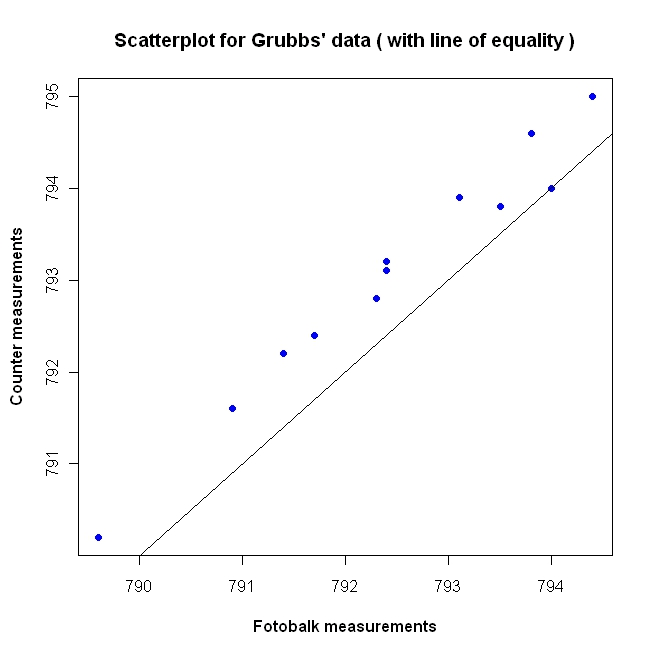
\includegraphics[width=125mm]{images/GrubbsScatter.jpeg}
  \caption{Scatter plot for Fotobalk and Counter methods.}\label{GrubbsScatter}
\end{center}
\end{figure}

\citet{Dewitte} notes that scatter plots were very seldom
presented in the Annals of Clinical Biochemistry. This apparently
results from the fact that the `Instructions for Authors' dissuade
the use of regression analysis, which conventionally is
accompanied by a scatter plot.

\subsection{Bland-Altman Plots}

In light of shortcomings associated with scatterplots,
\citet*{BA83} recommend a further analysis of the data. Firstly
case-wise differences of measurements of two methods $d_{i} =
y_{1i}-y_{2i}, \mbox{ for }i=1,2,\dots,n$, on the same subject
should be calculated, and then the average of those measurements, 
($a_{i} = (y_{1i} + y_{2i})/2 \mbox{ for }i=1,2,\dots, n$.

Following a technique known as the Tukey mean-difference plot, as noted by \citet{kozak2014including}
\citet{BA83} proposed that $a_i$ should be plotted against $d_i$, a plot now widely known as the Bland-Altman plot, and motivated this plot as follows:
\begin{quote}
``From this type of plot it is much easier to assess the magnitude
of disagreement (both error and bias), spot outliers, and see
whether there is any trend, for example an increase in (difference) for high values. This way of plotting the data is a very powerful way of displaying the results of a method comparison study."
\end{quote}

The case wise-averages capture several aspects of the data, such as expressing the range over which the values were taken, and assessing whether the assumptions of constant variance holds.
Case-wise averages also allow the case-wise differences to be presented on a two-dimensional plot, with better data visualization qualities than a one dimensional plot. \citet{BA86}
cautions that it would be the difference against either measurement value instead of their average, as the difference relates to both value. This approach has proved very popular, and the Bland-Altman plots is widely regarded as powerful graphical tool for making a visual assessment of the data.

The magnitude of the inter-method bias between the two methods is simply the average of the differences $\bar{d}$. This inter-method bias is represented with a line on the Bland-Altman plot. As the objective of the Bland-Altman plot is to advise on the agreement of two methods, the individual case-wise differences are also particularly relevant. The variances around this bias is estimated by the standard deviation of these differences $S_{d}$.

\subsubsection*{Rendering a Bland-Altma plot}
Construction of a Bland-Altman plot can be implemented easily with \texttt{R} packages such as Bendix Carstensen's \texttt{MethComp} package, which is designed to \textit{provide computational tools to manipulate, display and analyze data from method comparison studies} \citep{BXC2010}.

\subsection{Bland-Altman plots for the Grubbs data}

In the case of the Grubbs data the inter-method bias is $-0.61$ metres per second, and is indicated by the dashed line on Figure 1.2. By inspection of the plot, it is also possible to compare the precision of each method. Noticeably the differences tend to increase as the averages increase.


The Bland-Altman plot for comparing the `Fotobalk' and `Counter'
methods, which shall henceforth be referred to as the `F vs C'
comparison,  is depicted in Figure 1.2, using data from Table 1.3.
The presence and magnitude of the inter-method bias is indicated
by the dashed line.
\newpage

%Later it will be shown that case-wise differences are the sole
%component of the next part of the methodology, the limits of
%agreement.


\begin{table}[h!]
\renewcommand\arraystretch{0.7}%
\begin{center}
\begin{tabular}{|c||c|c||c|c|}
  \hline
 Round & Fotobalk  & Counter  & Differences  & Averages  \\
  &  [F] & [C] & [F-C] &  [(F+C)/2] \\
  \hline
1 & 793.8 & 794.6 & -0.8 & 794.2 \\
  2 & 793.1 & 793.9 & -0.8 & 793.5 \\
  3 & 792.4 & 793.2 & -0.8 & 792.8 \\
  4 & 794.0 & 794.0 & 0.0 & 794.0 \\
  5 & 791.4 & 792.2 & -0.8 & 791.8 \\
  6 & 792.4 & 793.1 & -0.7 & 792.8 \\
  7 & 791.7 & 792.4 & -0.7 & 792.0 \\
  8 & 792.3 & 792.8 & -0.5 & 792.5 \\
  9 & 789.6 & 790.2 & -0.6 & 789.9 \\
  10 & 794.4 & 795.0 & -0.6 & 794.7 \\
  11 & 790.9 & 791.6 & -0.7 & 791.2 \\
  12 & 793.5 & 793.8 & -0.3 & 793.6 \\
   \hline
\end{tabular}
\caption{Fotobalk and Counter methods: differences and averages.}
\end{center}
\end{table}

\begin{table}[h!]
\renewcommand\arraystretch{0.7}%
\begin{center}
\begin{tabular}{|c||c|c||c|c|}
  \hline
 Round & Fotobalk  & Terma  & Differences  & Averages  \\
  &  [F] & [T] & [F-T] &  [(F+T)/2] \\
  \hline
1 & 793.8 & 793.2 & 0.6 & 793.5 \\
  2 & 793.1 & 793.3 & -0.2 & 793.2 \\
  3 & 792.4 & 792.6 & -0.2 & 792.5 \\
  4 & 794.0 & 793.8 & 0.2 & 793.9 \\
  5 & 791.4 & 791.6 & -0.2 & 791.5 \\
  6 & 792.4& 791.6 & 0.8 & 792.0 \\
  7 & 791.7 & 791.6 & 0.1 & 791.6 \\
  8 & 792.3 & 792.4 & -0.1 & 792.3 \\
  9 & 789.6 & 788.5 & 1.1 & 789.0 \\
  10 & 794.4 & 794.7 & -0.3 & 794.5 \\
  11 & 790.9 & 791.3 & -0.4 & 791.1 \\
  12 & 793.5 & 793.5 & 0.0 & 793.5 \\

   \hline
\end{tabular}
\caption{Fotobalk and Terma methods: differences and averages.}
\end{center}
\end{table}

\newpage

\begin{figure}[h!]
\begin{center}
  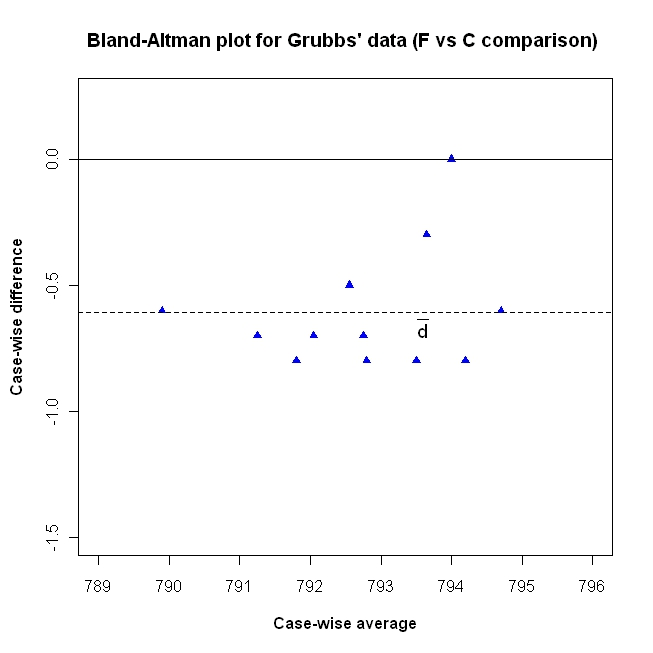
\includegraphics[width=120mm]{images/GrubbsBAplot-noLOA.jpeg}
  \caption{Bland-Altman plot For Fotobalk and Counter methods.}\label{GrubbsBA-noLOA}
\end{center}
\end{figure}



In Figure 1.3 Bland-Altman plots for the `F vs C' and `F vs T'
comparisons are shown, where `F vs T' refers to the comparison of
the `Fotobalk' and `Terma' methods. Usage of the Bland-Altman plot
can be demonstrate in the contrast between these comparisons. By inspection, there exists a larger inter-method bias in the `F vs C' comparison than in the `F vs T' comparison. Conversely there
appears to be less precision in `F vs T' comparison, as indicated
by the greater dispersion of covariates.

\begin{figure}[h!]
\begin{center}
  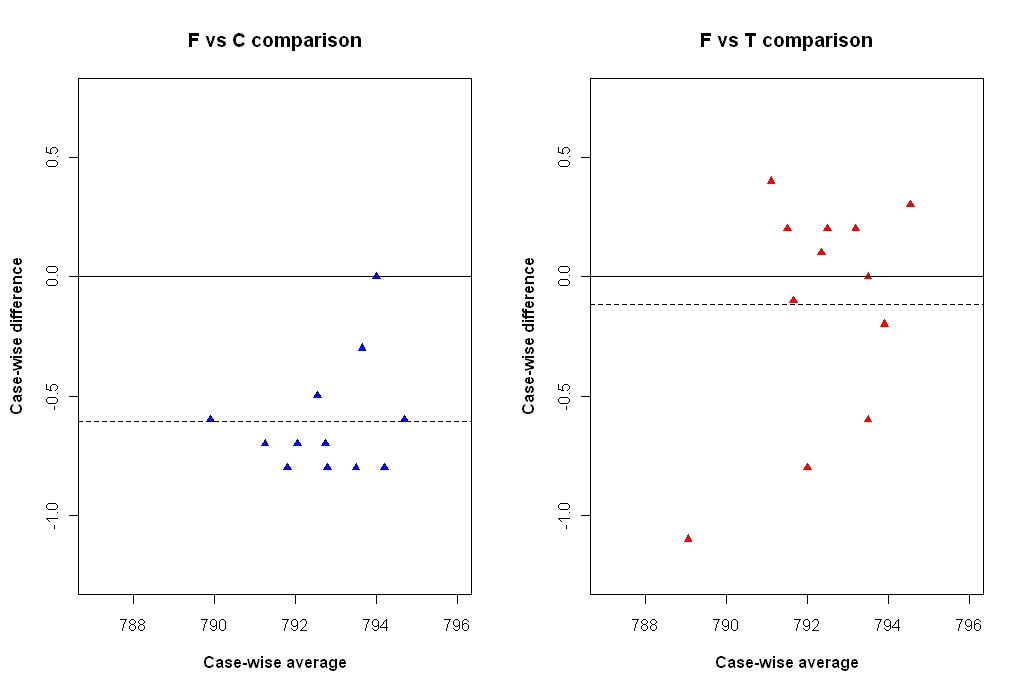
\includegraphics[height=90mm]{images/GrubbsDataTwoBAplots.jpeg}
  \caption{Bland-Altman plots for Grubbs' F vs C and F vs T comparisons.}\label{GrubbsDataTwoBAplots}
\end{center}
\end{figure}

\newpage


%\subfile{TechAcceptModel.tex}
\subsection{Adverse features}

Estimates for inter-method bias and variance of differences are only meaningful if there is uniform inter-bias and variability throughout the range of measurements. Fulfilment of these assumptions can be checked by visual inspection of the plot.The prototype Bland-Altman plots depicted in Figures 1.4, 1.5 and 1.6 are derived from simulated data, for the purpose of demonstrating how the plot would inform an analyst of features that would adversely affect use of the recommended approach.

Figure 1.4 demonstrates how the Bland-Altman plot would indicate
increasing variance of differences over the measurement range.
Fitted regression lines, for both the upper and lower half of the
plot, has been added to indicate the trend. Figure 1.5 is an
example of cases where the inter-method bias changes over the
measurement range. This is known as proportional bias, and is
defined by \citet{ludbrook97} as meaning that `one method gives
values that are higher (or lower) than those from the other by an
amount that is proportional to the level of the measured variable'. In both Figures 1.4 and 1.5, the assumptions necessary
for further analysis using the limits of agreement are violated.

Application of regression techniques to the Bland-Altman plot, and
subsequent formal testing for the constant variability of
differences is informative. The data set may be divided into two
subsets, containing the observations wherein the difference values
are less than and greater than the inter-method bias respectively.
For both of these fits, hypothesis tests for the respective slopes
can be performed. While both tests could be considered separately,
multiple comparison procedures, such as the Benjamini-Hochberg
\citep{BH} test, are advisable.

\begin{figure}[h!]
\begin{center}
  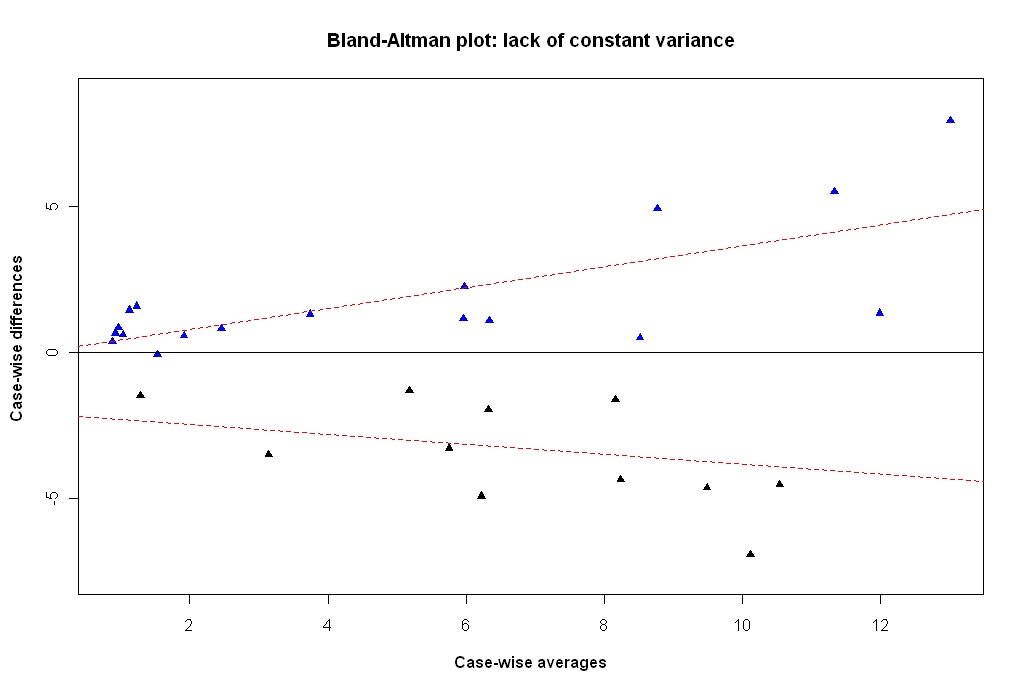
\includegraphics[height=90mm]{images/BAFanEffect.jpeg}
  \caption{Bland-Altman plot demonstrating the increase of variance over the range.}\label{BAFanEffect}
\end{center}
\end{figure}

\begin{figure}[h!]
\begin{center}
  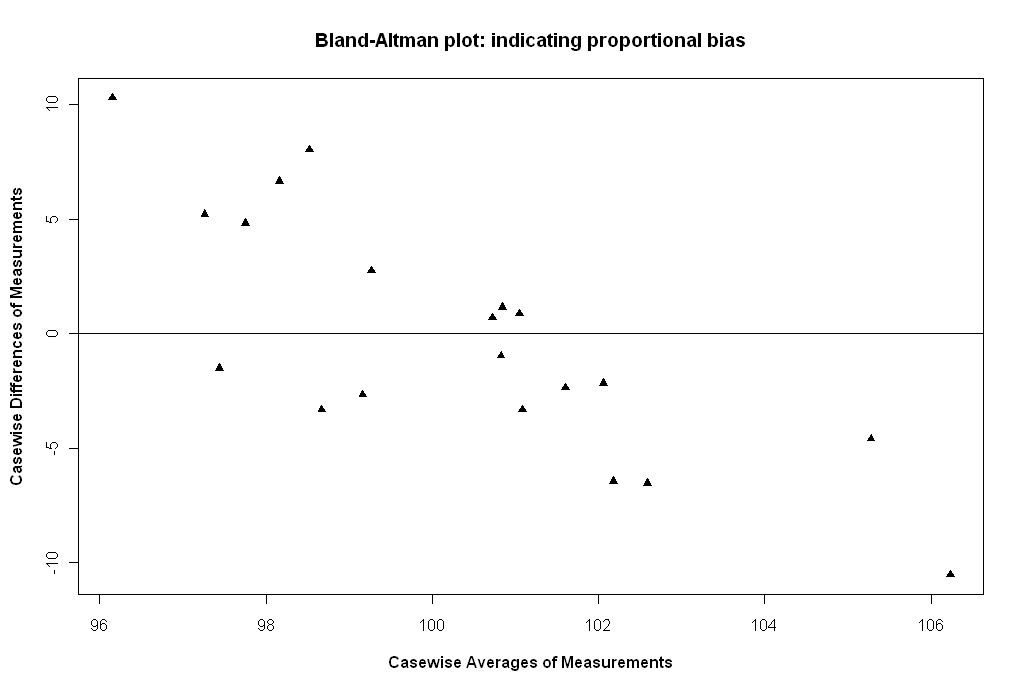
\includegraphics[height=90mm]{images/PropBias.jpeg}
  \caption{Bland-Altman plot indicating the presence of proportional bias.}\label{PropBias}
\end{center}
\end{figure}

\begin{figure}[h!]
\begin{center}
  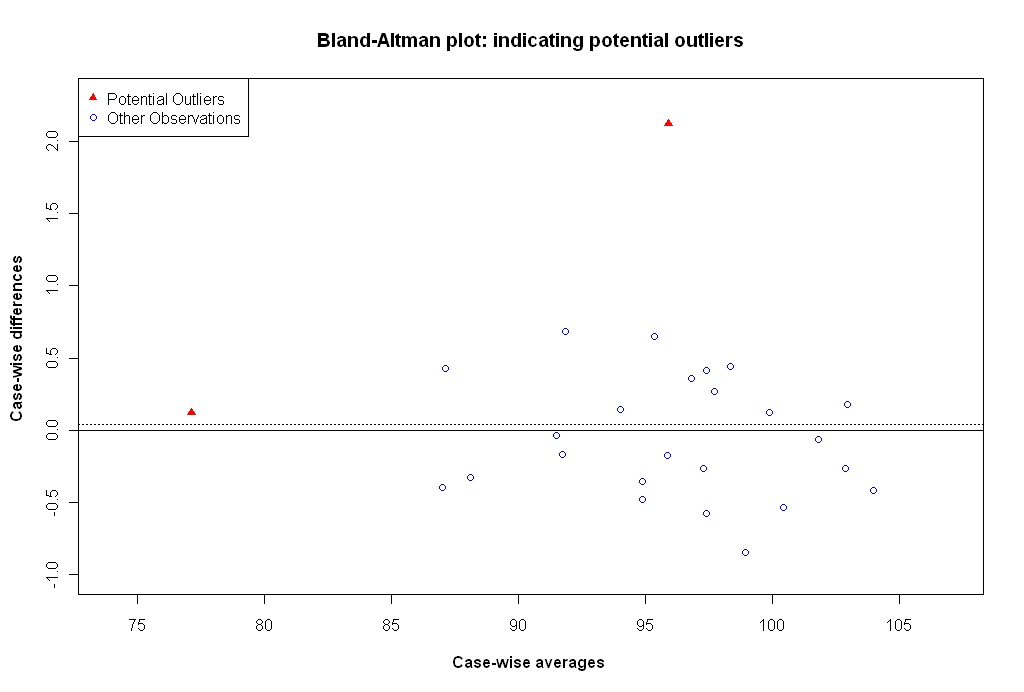
\includegraphics[width=125mm]{images/BAOutliers.jpeg}
  \caption{Bland-Altman plot indicating the presence of potential outliers.}\label{Outliers}
\end{center}
\end{figure}

\newpage


The Bland-Altman plot also can be used to identify outliers. An
outlier is an observation that is conspicuously different from the
rest of the data that it arouses suspicion that it occurs due to a
mechanism, or conditions, different to that of the rest of the
observations. \citet*{BA99} do not recommend excluding outliers from analyses,
but remark that recalculation of the inter-method bias estimate,
and further calculations based upon that estimate, are useful for
assessing the influence of outliers. The authors remark that `we
usually find that this method of analysis is not too sensitive to
one or two large outlying differences'. Figure 1.6 demonstrates how the Bland-Altman
plot can be used to visually inspect the presence of potential
outliers.

As a complement to the Bland-Altman plot, \citet{Bartko} proposes
the use of a bivariate confidence ellipse, constructed for a
predetermined level. \citet{AltmanEllipse} provides the relevant calculations for the
ellipse. This ellipse is intended as a visual
guidelines for the scatter plot, for detecting outliers and to
assess the within- and between-subject variances.

The minor axis relates to the between subject variability, whereas
the major axis relates to the error mean square, with the ellipse
depicting the size of both relative to each other.
Consequently Bartko's ellipse provides a visual aid to determining the
relationship between variances. If $\mbox{var}(a)$ is greater than $\mbox{var}(d)$, the orientation of the ellipse is horizontal. Conversely if $\mbox{var}(a)$ is less than $\mbox{var}(d)$, the orientation of the ellipse is vertical.


%(Furthermore \citet{Bartko}
%proposes formal testing procedures, that shall be discussed in due
%course.)

The Bland-Altman plot for the Grubbs data, complemented by Bartko's ellipse, is depicted in Figure 1.7.
The fourth observation is shown to be outside the bounds of the ellipse, indicating that it is a potential outlier.


\begin{figure}[h!]
  % Requires \usepackage{graphicx}
  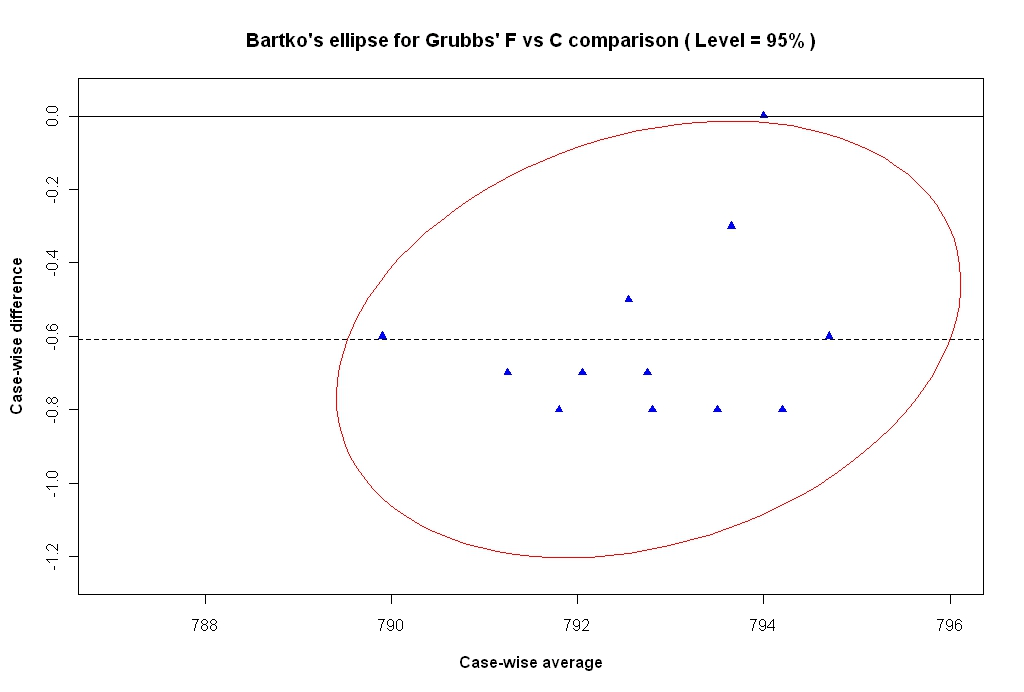
\includegraphics[width=130mm]{images/GrubbsBartko.jpeg}
  \caption{Bartko's Ellipse for Grubbs' data.}\label{GrubbsBartko}
\end{figure}

The limitations of using bivariate approaches to outlier detection
in the Bland-Altman plot can demonstrated using Bartko's ellipse.
A covariate is added to the `F vs C' comparison that has a
difference value equal to the inter-method bias, and an average
value that markedly deviates from the rest of the average values
in the comparison, i.e. 786. Table 1.8 depicts a $95\%$ confidence
ellipse for this manipulated data set. By inspection of the
confidence interval, we would conclude that this extra
covariate is an outlier, in spite of the fact that this
observation is very close to the inter-method bias as determined by this approach.

\begin{figure}[h!]
  % Requires \usepackage{graphicx}
  \includegraphics[width=130mm]{images/GrubbsBartko2.jpeg}
  \caption{Bartko's Ellipse for Grubbs' data, with an extra covariate.}\label{GrubbsBartko2}
\end{figure}


Importantly, outlier classification must be informed by the logic of the
mechanism that produces the data. In the Bland-Altman plot, the horizontal displacement (i.e. the average) of any
observation is supported by two separate measurements. Any
observation should not be considered an outlier on the basis of a
noticeable horizontal displacement from the main cluster, as in
the case with the extra covariate. Conversely, the fourth
observation, from the original data set, should be considered an
outlier, as it has a noticeable vertical displacement from the
rest of the observations.

%Grubbs' test is a statistical test used for detecting outliers in a
%univariate data set that is assumed to be normally distributed.

%\citet{Grubbs} defined an outlier as a co-variate that appears to
%deviate markedly from other members of the sample in which it
%occurs.

In classifying whether a observation from a univariate data set is
an outlier, many formal tests are available, such as the Grubbs test for outliers. In assessing
whether a covariate in a Bland-Altman plot is an outlier, this
test is useful when applied to the case-wise difference values treated as a
univariate data set. The null hypothesis of the Grubbs test procedure is the absence
of any outliers in the data set. Conversely, the alternative hypotheses is that there is at least one outlier
present.

The test statistic for the Grubbs test ($G$) is the largest
absolute deviation from the sample mean divided by the standard
deviation of the differences,
\begin{equation}
G =  \displaystyle\max_{i=1,\ldots, n}\frac{\left \vert d_i -
\bar{d}\right\vert}{S_{d}}.
\end{equation}

For the `F vs C' comparison it is the fourth observation gives
rise to the test statistic, $G = 3.64$. The critical value is
calculated using Student's $t$ distribution and the sample size,
\[
U = \frac{n-1}{\sqrt{n}} \sqrt{\frac{t_{\alpha/(2n),n-2}^2}{n - 2
+ t_{\alpha/(2n),n-2}^2}}.
\]
For this test $U = 0.75$. The conclusion of this test is that the fourth observation in the `F vs C' comparison is an outlier, with $p-$value = 0.003, in accordance with the previous result of Bartko's ellipse.


\section{Limits of Agreement}
% introduces
A third element of the Bland-Altman approach, an interval known
as `limits of agreement' is introduced in \citet*{BA86}
(sometimes referred to in literature as 95\% limits of agreement).
Limits of agreement are used to assess whether the two methods of
measurement can be used interchangeably. \citet{BA86} refer to
this as the `equivalence' of two measurement methods. The specific question to which limits of
agreement are intended as the answer to must be
established clearly. \citet*{BA95} comment that the limits of agreement show `how
far apart measurements by the two methods were likely to be for
most individuals', a definition echoed in their 1999 paper:

\begin{quote}``We can then say that nearly all pairs
of measurements by the two methods will be closer together than
these extreme values, which we call 95\% limits of agreement.
These values define the range within which most differences
between measurements by the two methods will lie."
\end{quote}

The limits of agreement (LoA) are computed by the following
formula:
\[
LoA = \bar{d} \pm 1.96 s_{d}
\]
with $\bar{d}$ as the estimate of the inter method bias, $s_{d}$
as the standard deviation of the differences and 1.96 (sometimes rounded to 2) is the 95\%
quantile for the standard normal distribution. The limits of agreement methodology assumes a constant level of bias throughout the range of measurements. Importantly the authors recommend prior determination of what would constitute acceptable
agreement, and that sample sizes should be predetermined to give an accurate conclusion. However \citet{mantha} highlight inadequacies in the correct application of limits of agreement, resulting in contradictory estimates of limits of agreement in various papers.

%\begin{quote}
%``How far apart measurements can be without causing difficulties
%will be a question of judgment. Ideally, it should be defined in
%advance to help in the interpretation of the method comparison and
%to choose the sample size \citep{BA86}".
%\end{quote}


For the Grubbs `F vs C' comparison, these limits
of agreement are calculated as -0.132 for the upper bound, and
-1.08 for the lower bound. Figure 1.9 shows the resultant
Bland-Altman plot, with the limits of agreement shown in dashed
lines.


\begin{figure}[h!]
\begin{center}
  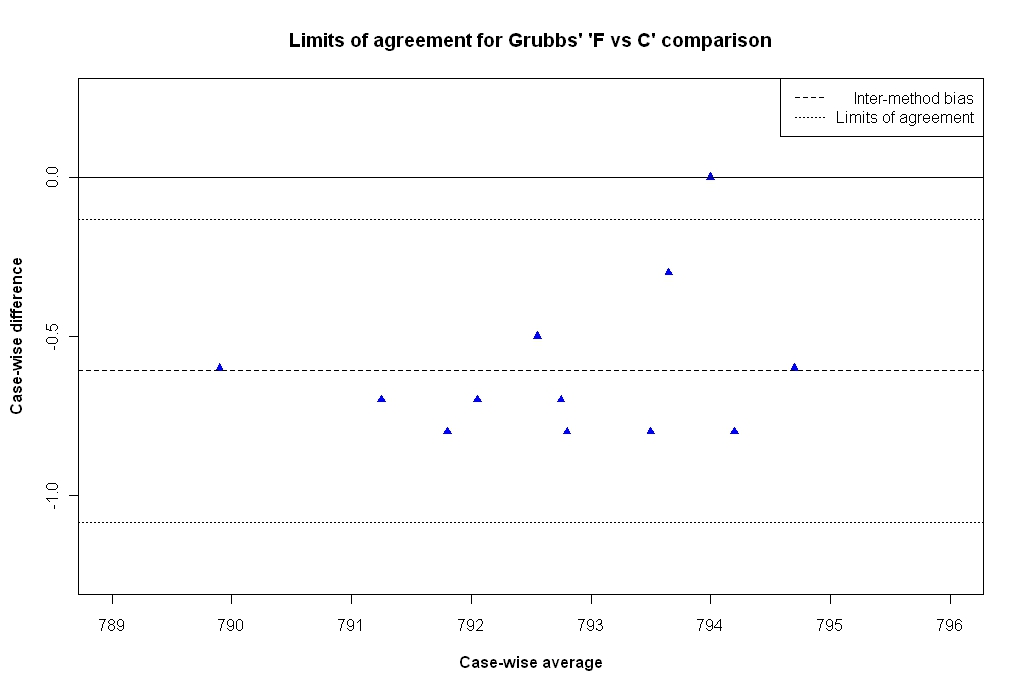
\includegraphics[width=125mm]{images/GrubbsBAplot-LOA.jpeg}
  \caption{Bland-Altman plot with limits of agreement}\label{GrubbsBAplot-noLOA}
\end{center}
\end{figure}

%But as \citet*{BA86} point out this may not be the case. Variants of the limits of agreement that overcome this
% problem shall be introduced in due course.

\subsection{Inferences on Bland-Altman estimates}
\citet*{BA99} advises on how to calculate confidence intervals for the inter-method bias and limits of agreement.
For the inter-method bias, the confidence interval is a simply that of a mean: $\bar{d} \pm t_{(\alpha/2,n-1)} S_{d}/\sqrt{n}$.
The confidence
intervals and standard error for the limits of agreement follow from the variance of the limits of agreement, which is shown to be

 \[
  \mbox{Var}(LoA) = (\frac{1}{n}+\frac{1.96^{2}}{2(n-1)})s_{d}^{2}.
 \]

If $n$ is sufficiently large this can be following approximation
can be used
 \[
  \mbox{Var}(LoA) \approx 1.71^{2}\frac{s_{d}^{2}}{n}.
 \]
Consequently the standard errors of both limits can be
approximated as $1.71$ times the standard error of the
differences.

A $95\%$ confidence interval can be determined, by means of the
\emph{t} distribution with $n-1$ degrees of freedom. However, \citet*{BA99} comment that such calculations  may be `somewhat optimistic' on account of the associated assumptions not being realized.

%\subsubsection{Small Sample Sizes} The limits of agreement are
%estimates derived from the sample studied, and will differ from
%values relevant to the whole population, hence the importance of a
%suitably large sample size. A different sample would give
%different limits of agreement. Student's t-distribution is a well
%known probability distribution used in statistical inference for
%normally distributed populations when the sample size is small
%\citep{student,Fisher3}. Consequently, using 't' quantiles , as
%opposed to standard normal quantiles, may give a more appropriate
%calculation for limits of agreement when the sample size is small.
%For sample size $n=12$ the `t' quantile is 2.2 and the limits of
%agreement are (-0.074,-1.143).


\subsection{Formal definition of limits of agreement}
\citet{BA99} note the similarity of limits of agreement to
confidence intervals, but are clear that they are not the same
thing. Interestingly, they describe the limits as `being like a
reference interval'.

Limits of agreement have very similar construction to Shewhart
control limits. The Shewhart chart is a well known graphical
methodology used in statistical process control. Consequently
there is potential for misinterpreting the limits of agreement as
they were Shewhart control limits. 
%Importantly the
%parameters used to determine the Shewhart limits are time ordered, based on the process's historical values, a key difference with Bland-Altman limits of agreement.

\citet{BXC2008} regards the limits of agreement as a prediction
interval for the difference between future measurements with the
two methods on a new individual, but states that it does not fit
the formal definition of a prediction interval, since the
definition does not consider the errors in estimation of the
parameters. Prediction intervals, which are often used in
regression analysis, are estimates of an interval in which future
observations will fall, with a certain probability, given what has
already been observed. \citet{BXC2008} offers an alternative
formulation, a $95\%$ prediction interval for the difference
\[
\bar{d} \pm t_{(0.025, n-1)}s_{d} \sqrt{1+\frac{1}{n}}
\]

\noindent where $n$ is the number of subjects. Carstensen is
careful to consider the effect of the sample size on the interval
width, adding that only for 61 or more subjects is the
quantile less than 2.

\citet{luiz} offers an alternative description of limits of
agreement, this time as tolerance limits. A tolerance interval for
a measured quantity is the interval in which a specified fraction
of the population's values lie, with a specified level of
confidence. \citet{Barnhart} describes them as a probability
interval, and offers a clear description of how they should be
used; `if the absolute limit is less than an acceptable difference
$d_{0}$, then the agreement between the two methods is deemed
satisfactory'.

The prevalence of contradictory definitions of what limits of agreement strictly are will inevitably attenuate the poor standard of reporting using limits of agreement, as mentioned by \citet{mantha}.

%At least 100 historical
%values must be used to determine the acceptable value (i.e the
%process mean) and the process standard deviation. The principle
%that the mean and variance of a large sample of a homogeneous
%population is a close approximation of the population's mean and
%variance justifies this.

%\begin{figure}[h!]
%\begin{center}
%  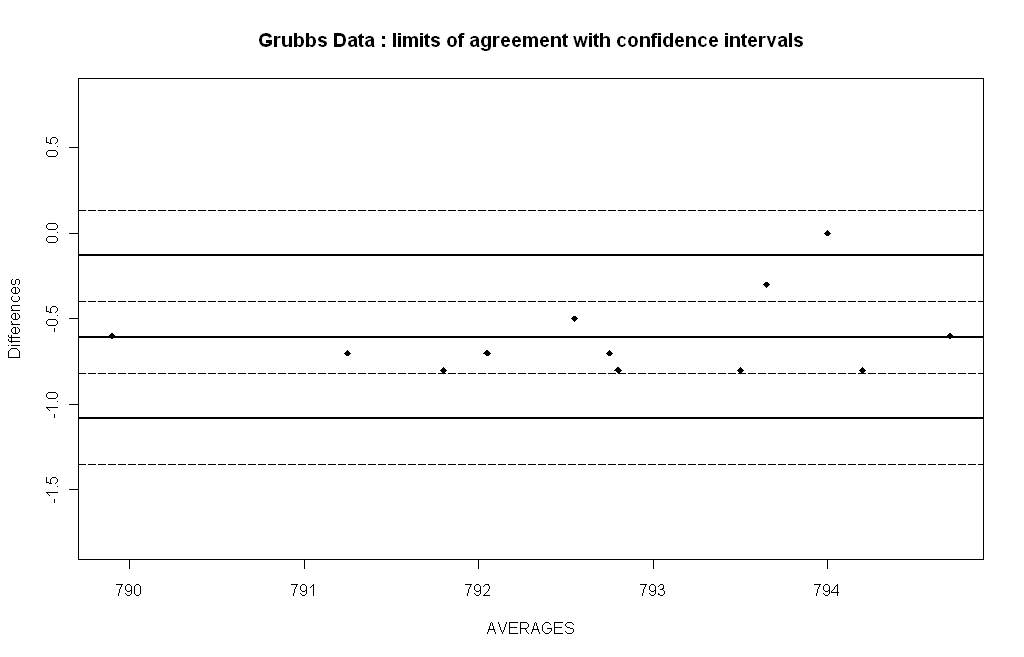
\includegraphics[width=125mm]{GrubbsLOAwCIs.jpeg}
%  \caption{Limits of agreement with confidence intervals}\label{LOAwCIs}
%\end{center}
%\end{figure}

%\newpage
%\section{Agreement Indices}
%\citet{Barnhart} provided an overview of several agreement
%indices, including the limits of agreement. Other approaches, such
%as mean squared deviation, the tolerance deviation index and
%coverage probability are also discussed.

\subsection{Alternative Agreement Indices}
As an alternative to limits of agreement, \citet{lin2002} proposes the use of
the mean square deviation in assessing agreement. The mean square
deviation is defined as the expectation of the squared differences
of two readings. The MSD is usually used for the case of two
measurement methods $X$ and $Y$, each making one measurement for
the same subject, and is given by
\[
MSDxy = E[(x - y)^2]  = (\mu_{x} - \mu_{y})^2 + (\sigma_{x} -
\sigma_{y})^2 + 2\sigma_{x}\sigma_{y}(1-\rho_{xy}).
\]


\citet{Barnhart} advises the use of a predetermined upper limit
for the MSD value, $MSD_{ul}$, to define satisfactory agreement.
However, a satisfactory upper limit may not be easily
determinable, thus creating a drawback to this methodology.


Alternative indices, proposed by \citet{Barnhart}, are the square root of the MSD and the expected absolute difference (EAD). 
\[
EAD = E(|x - y|) = \frac{\sum |x_{i}- y_{i}|}{n}
\]


Both of these indices can be interpreted intuitively, since their units are the same as that of the original measurements. Also they can be compared to the maximum acceptable absolute difference between two methods of measurement $d_{0}$. For the sake of brevity, the EAD will be considered solely.

The EAD can be used to supplement the inter-method bias in an
initial comparison study, as the EAD is informative as a measure
of dispersion, is easy to calculate and requires no distributional
assumptions. A consequence of using absolute differences is that high variances would result in a higher EAD value. 

% latex table generated in R 3.1.1 by xtable 1.7-4 package
% Mon Feb 23 21:12:33 2015
% latex table generated in R 3.1.1 by xtable 1.7-4 package
% Mon Feb 23 21:13:45 2015
% latex table generated in R 3.1.1 by xtable 1.7-4 package
% Mon Feb 23 22:10:26 2015
%\begin{table}[ht]
%	\centering
%	\begin{tabular}{r| rrrr}
%		\hline
%		\item & X & Y & U & V \\ 
%		\hline
%		1 & 101.83 & 102.52 & 98.05 & 99.53 \\ 
%		2 & 101.68 & 102.69 & 99.17 & 96.53 \\ 
%		3 & 97.89 & 99.01 & 100.31 & 97.55 \\ 
%		4 & 98.15 & 99.57 & 100.35 & 96.03 \\ 
%		5 & 99.94 & 100.85 & 99.51 & 99.00 \\ 
%		6 & 98.85 & 98.86 & 98.50 & 100.76 \\ 
%		7 & 99.86 & 97.85 & 100.66 & 99.37 \\ 
%		8 & 101.57 & 100.21 & 99.66 & 108.87 \\ 
%		9 & 100.12 & 99.85 & 99.70 & 105.16 \\ 
%		10 & 99.49 & 98.77 & 101.55 & 94.31 \\ 
%		\hline
%	\end{tabular}
%\end{table}




\begin{table}[ht]
	\centering
	\begin{tabular}{|c|c|c|c|c|}
		\hline
		& U & V & $U-V$ & $|U-V|$ \\ 
		\hline
		1 & 98.05 & 99.53 & -1.49 & 1.49 \\ 
		2 & 99.17 & 96.53 & 2.64 & 2.64 \\ 
		3 & 100.31 & 97.55 & 2.75 & 2.75 \\ 
		4 & 100.35 & 96.03 & 4.32 & 4.32 \\ 
		5 & 99.51 & 99.00 & 0.51 & 0.51 \\ 
		6 & 98.50 & 100.76 & -2.26 & 2.26 \\ 
		7 & 100.66 & 99.37 & 1.29 & 1.29 \\ 
		8 & 99.66 & 108.87 & -9.21 & 9.21 \\ 
		9 & 99.70 & 105.16 & -5.45 & 5.45 \\ 
		10 & 101.55 & 94.31 & 7.24 & 7.24 \\ 
		\hline
	\end{tabular}
	\caption{Example data set}
	\label{EADdata}
\end{table}

To illustrate the use of EAD, consider table ~\ref{EADdata}. The inter-method bias is 0.03, which is quite close to zero, which is desirable in the context of agreement. However, an identity plot would indicate very poor agreement, as the points are noticeably distant from the line of equality.
\begin{figure}
\centering
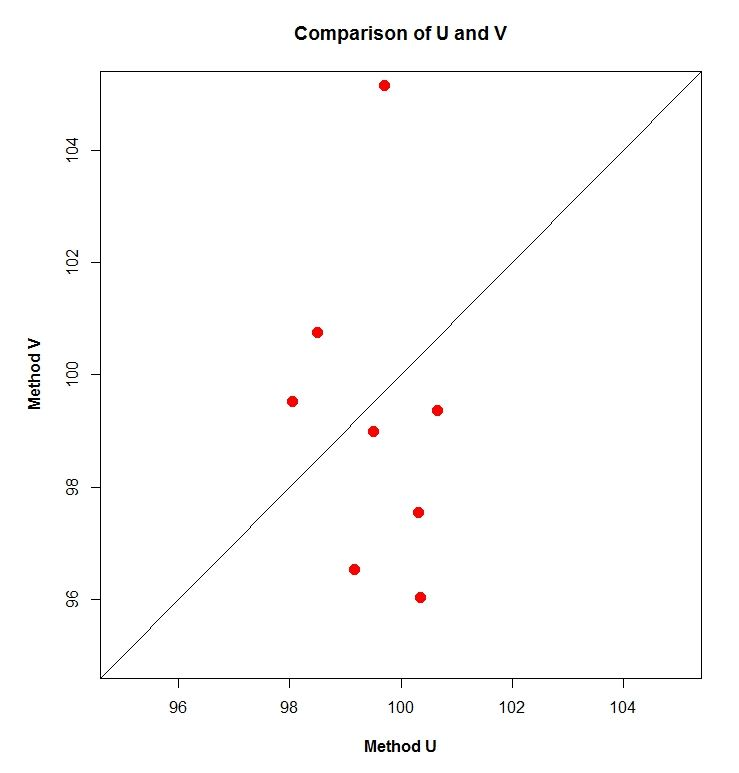
\includegraphics[width=0.7\linewidth]{EAD-UV}
\caption{Identity Plot for example data}
\label{fig:EADidentity}
\end{figure}

The limits of agreement are $[-9.61, 9.68]$, a wide interval for this data. As with the identity plot, this would indicate lack of agreement. As with inter-method bias, an EAD value close to zero is desirable. However, from table ~\ref{EADdata}, the EAD can be computed as 3.71. The Bland-Altman plot remains a useful part of the analysis. In \ref{fig:EAD1}, it is clear there is a systematic decrease in differences across the range of measurements.
\begin{figure}
	\centering
	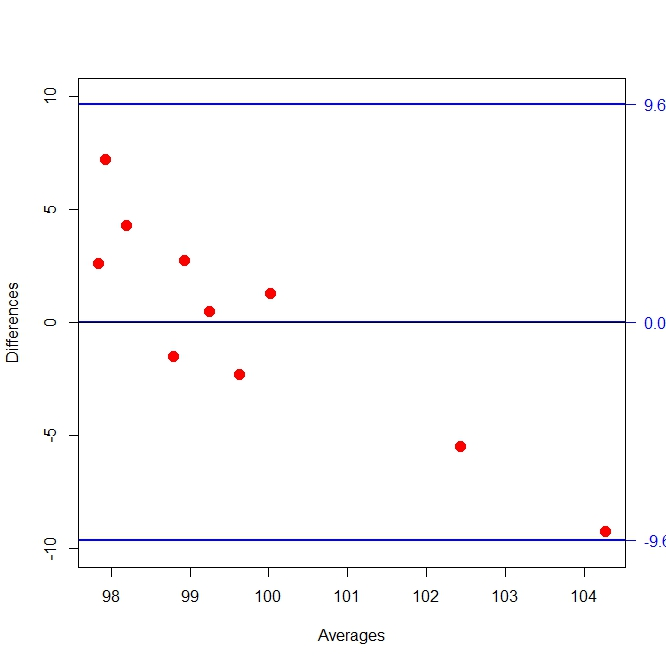
\includegraphics[width=0.7\linewidth]{images/EAD1}
	\caption{Bland-Altman Plot for UV comparison}
	\label{fig:EAD1}
\end{figure}

\citet{Barnhart} remarks that a comparison of EAD and MSD , using
simulation studies, would be interesting, while further adding
that `\textit{It will be of interest to investigate the benefits of these
possible new unscaled agreement indices}'. For the Grubbs' `F vs C' and `F vs T' comparisons, the inter-method bias, difference variances, limits of agreement and EADs are shown
in Table 1.5. The corresponding Bland-Altman plots for `F vs C' and `F vs T' comparisons were depicted previously on Figure 1.3. While the inter-method bias for the `F vs T' comparison is smaller, the EAD penalizes the comparison for having a greater variance of differences. Hence the EAD values for both comparisons are much closer.
\begin{table}[ht]
\begin{center}
\begin{tabular}{|c|c|c|}
  \hline
 & F vs C & F vs T  \\
  \hline
Inter-method bias & -0.61 & 0.12 \\ \hline
Difference variance & 0.06 & 0.22  \\ \hline 
Limits of agreement & (-1.08,	-0.13) & (-0.81,1.04) \\
  EAD & 0.61 & 0.35  \\ \hline 
   \hline
\end{tabular}
\caption{Agreement indices for Grubbs' data comparisons.}
\end{center}
\end{table}

Further to  \citet{lin2000} and \citet{lin2002}, individual agreement between two measurement methods may be
assessed using the the coverage probability (CP) criteria or the total deviation index (TDI). If $d_{0}$ is predetermined as the maximum acceptable absolute difference between two methods of measurement, the probability that the absolute difference of two measures being less than $d_{0}$ can be computed. This is known as the coverage probability (CP).

\begin{equation}
CP = P(|x_{i} - y_{i}| \leq d_{0})
\end{equation}

If $\pi_{0}$ is set as the predetermined coverage probability, the
boundary under which the proportion of absolute differences is
$\pi_{0}$ may be determined. This boundary is known as the `total
deviation index' (TDI). Hence the TDI is the $100\pi_{0}$
percentile of the absolute difference of paired observations.
\subsection{Prevalence of the Bland-Altman plot}
%---------------------------------------------%

\citet*{BA86}, which further develops the Bland-Altman methodology,
was found to be the sixth most cited paper of all time by the
\citet{BAcite}. \cite{Dewitte} describes the rate at which
prevalence of the Bland-Altman plot has developed in scientific
literature. \citet{Dewitte} reviewed the use of Bland-Altman plots
by examining all articles in the journal `Clinical Chemistry'
between 1995 and 2001. This study concluded that use of the
Bland-Altman plot increased over the years, from 8\% in 1995 to
14\% in 1996, and 31-36\% in 2002.

The Bland-Altman Plot has since become expected, and
often obligatory, approach for presenting method comparison
studies in many scientific journals \citep{hollis}. Furthermore
\citet{BritHypSoc} recommend its use in papers pertaining to
method comparison studies for the journal of the British
Hypertension Society.

%% TAM
\section{The Technology Acceptance Model}
Davis (1989) proposes the TAM model, which suggests an hypothesis as to why users may adopt particular technologies, and not others. 
According to this theory, when users are presented with a new 
technology, two important factors will influence their decision about how and when they will adopt it.
\begin{description}
	\item[Perceived usefulness (PU)] - This was defined by Fred Davis as "the degree to which a person believes that using a particular system would enhance his or her job performance".
	\item[Perceived ease-of-use (PEOU)] - Davis defined this as "the degree to which a person believes that using a particular system would be free from effort" 
\end{description}

Davis's explanations of these term can be rephrased for application to statistical analysis. 
Perceived Use could refer to the degree to which an user would deem a particular statistical method would properly establish the results of an analaysis. In the case of method comparison studies, proper indication of agreement, or lack thereof.


Perceived ease-of-use requires only applying the context of a satistical problem. A very modest statistical skill set is the only prerequistive for constructing a Bland-Altman plot, and computing limits of agreement. The main building blocks 
are simple descriptive, statistics and a knowledge of the normal distribution. These are topics that feature in almost every undergraduate statistics courses. Furthermore \citet{kikozak2014including} recommends including the Bland-Altman method itself in undergraduate teaching.
%---------------------------------------------%

In short, the user perceives the Bland-Altman methodology to be an easy-to-implement technique, that will properly address the question of agreement.

Conversely the Survival plot is a derivative of the Kaplan-Meier Curve, a non-parametric graphical technique that features in Survival Analysis. This subject area is a well known domain of statistics, but would be encountered 
on curriculums of specialist courses. 

The Mountain Plot is formally called the empirical folder cumulative distribution plot. While not particularly hard to render, the procedure is not straight-forward for the casual user. Currently there is only one software implementation, \textbf{\textit{medcalc.be}} toolkit.
	\section{Variations and Alternative Graphical Methods}
	In this section, we will look at some variations and enhancements of the Bland-Altman plot, as well as some alternative graphcial techniques. Strictly speaking, the Identity Plot is advised by Bland and Altman as a prior analysis to the Bland-Alman plot, and therefore is neither a variant nor an alternative approach. However it is worth mentioning, as it is a simple, powerful and elegant technique that is often overlooked in method comparison studies. The identity plot is a simple scatter-plot approach of measurements for both methods on either axis, with the line of equality (the $X=Y$ line, i.e. the 45 degree line through the origin). This plot can gives the analyst a cursory examination of how well the measurement methods agree. In the case of good agreement, the covariates of the plot accord closely with the line of equality.
	
	\subsection{Variants of the Bland-Altman Plot}
	In light of some potential pitfalls associated with the conventional difference plot, a series of alternative formulations for the Bland-Altman approach have been proposed.
	
	Referring to the assumption that bias and variability are constant across the range
	of measurements, \citet{BA99} address the case where there is an increase in variability as the magnitude increases. They remark 	that it is possible to ignore the issue altogether, but the limits of agreement would be wider apart than necessary when just lower magnitude measurements are considered. Conversely the limits would be too narrow should only higher magnitude measurements be used.	To address the issue, they propose the logarithmic transformation of the data. The plot is then formulated as the difference of paired log values against their mean. Bland and Altman acknowledge that this is not easy to interpret, and may not be suitable in all cases.
	
	\subsubsection*{Bland and Altman's Percentage and Ratio Plots}
	%------------------------------------------------------------- %
	\citet{BA99} offer two variations of the Bland-Altman plot intended to overcome situations where the conventional plot is inappropriate. The first variation is a plot of casewise differences as percentage of averages, and is appropriate when the variability of the differences increase as the
	magnitude increases. 
	
	%------------------------------------------------------------- %
	% % RATIO / EKSBORG
	The second variation is a plot of casewise ratios as percentage of averages. This will remove the need for
	logarithmic transformation. This approach is useful when there is an increase in variability of the differences as the magnitude of the measurement increases. \citet{Eksborg} proposed such a ratio plot,
	independently of Bland and Altman. \citet{Dewitte} commented on
	the reception of this article by saying `\textit{Strange to say, this 
		report has been overlooked}'.
	
	
	%	%----------------------------------------------------------------%
	%	\section{Dewitte et al }
	%	\begin{quote}When the standard deviation increases with concentration, Bland and Altman recommend a logarithmic y scale, whereas others propose a percent y scale (Pollock et al, 2002). Although generally there is not much difference in effect between using percentages and using a log transformation of the data, we prefer the percent plot (except when data extend over several orders of magnitude) because numbers can be read directly from the plot without the need for back-transformation.
	%	\end{quote}
	%	
	%	\begin{verbatim}
	%	absolute - small range
	%	percentage - medium range
	%	log scale - large range
	%	\end{verbatim}
	%==================================================== %

	%%%%%%%%%%%%%%%%%%%%%%%%%%%%%%%%%%%%%%%%%%%%%%%%%%%%%%%%%%%%%%%%%%%%%%%%%%%%%%%%%%%%%%%%%%%%%%%%%%%%%%%%%%%%%%%%%%%%%%%%
	
	\subsubsection{Bartko's Ellipse}
	
	As an enhancement on the Bland Altman Plot, \citet{Bartko} has
	expounded a confidence ellipse for the covariates. \citet{Bartko} proposes
	a bivariate confidence ellipse as a boundary for dispersion. The stated purpose is to `amplify dispersion', which presumably is for  the purposes of outlier detection. The orientation of the the ellipse is key to interpreting the results. The minor axis is related to the between-item variability whereas the major axis is related to the mean squared error (referred to here as Error Mean Square).The ellipse illustrates the size of both relative to each
	other. 
	
	
	Consequently Bartko's ellipse provides a visual aid to determining the
	relationship between variances. 
	Furthermore, the ellipse provides a visual aid to determining the relationship
	between the variance of the means $Var(a_{i})$ and the variance of the differences $Var(d_{i})$. If $\mbox{var}(a)$ is greater than $\mbox{var}(d)$, the orientation of the ellipse is horizontal. Conversely if $\mbox{var}(a)$ is less than $\mbox{var}(d)$, the orientation of the ellipse is vertical. The more horizontal the ellipse, the greater the degree of agreement between the two methods being tested.
	
	
	%(Furthermore \citet{Bartko}
	%proposes formal testing procedures, that shall be discussed in due
	%course.)
	Bartko states that the ellipse can, inter alia, be used to detect the presence of outliers (furthermore
	\citet{Bartko} proposes formal testing procedures, that shall be discussed in due course). 
	The Bland-Altman plot for the Grubbs data, complemented by Bartko's ellipse, is depicted in Figure ~\ref{GrubbsBartko1}.
	The fourth observation is shown to be outside the bounds of the ellipse, indicating that it is a potential outlier.
	
	
	\begin{centering}
		\begin{figure}[h!]
			% Requires \usepackage{graphicx}
			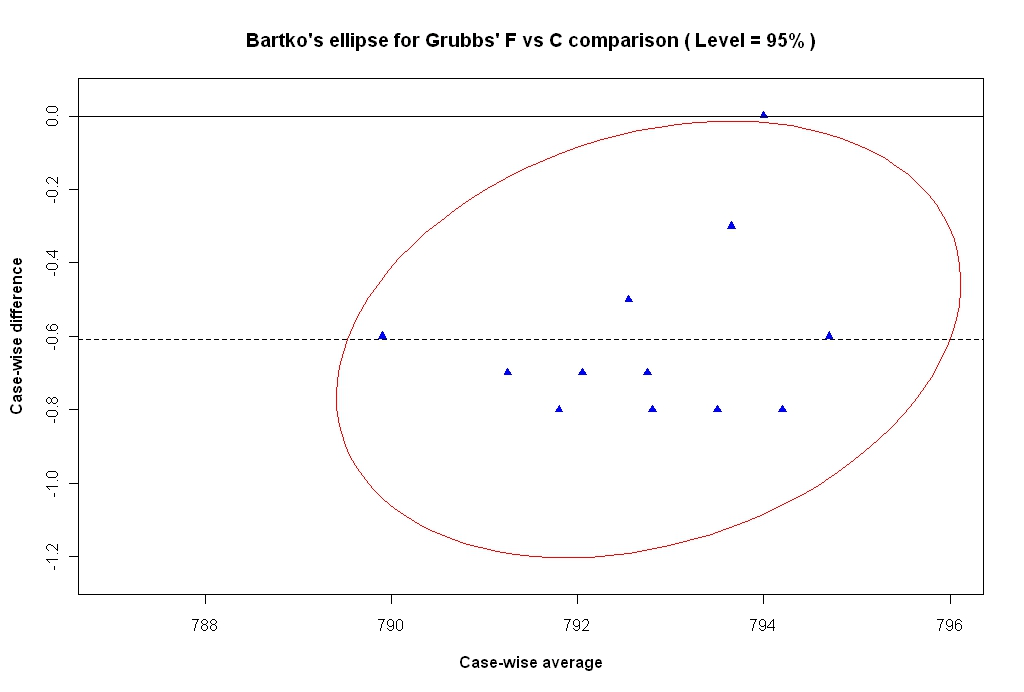
\includegraphics[width=130mm]{images/GrubbsBartko.jpeg}
			\caption{Bartko's Ellipse For Grubbs' Data.}
			\label{GrubbsBartko1}
		\end{figure}
	\end{centering}
	
	The limitations of using bivariate approaches to outlier detection
	in the Bland-Altman plot can demonstrated using Bartko's ellipse.
	A covariate is added to the `F vs C' comparison that has a
	difference value equal to the inter-method bias, and an average
	value that markedly deviates from the rest of the average values
	in the comparison, i.e. 786. Table 1.8 depicts a $95\%$ confidence
	ellipse for this manipulated data set. By inspection of the
	confidence interval, a conclusion would be reached that this extra
	covariate is an outlier, in spite of the fact that this
	observation is wholly consistent with the conclusion of the
	Bland-Altman plot.
	
	%\begin{figure}[h!]
	%  % Requires \usepackage{graphicx}
	%  \includegraphics[width=130mm]{GrubbsBartko2.jpeg}
	%  \caption{Bartko's Ellipse For Grubbs' Data, with an extra covariate.}\label{GrubbsBartko2}
	%\end{figure}
	
	
	Importantly, outlier classification must be informed by the logic of the
	data's formulation. In the Bland-Altman plot, the horizontal displacement of any
	observation is supported by two independent measurements. Any
	observation should not be considered an outlier on the basis of a
	noticeable horizontal displacement from the main cluster, as in
	the case with the extra covariate. Conversely, the fourth
	observation, from the original data set, should be considered an
	outlier, as it has a noticeable vertical displacement from the
	rest of the observations.
	\newpage
	
	\begin{figure}[h!]
		% Requires \usepackage{graphicx}
		\includegraphics[width=130mm]{images/GrubbsBartko2.jpeg}
		\caption{Bartko's Ellipse For Grubbs' Data, with an extra covariate.}\label{GrubbsBartko2}
	\end{figure}
	
	In the Bland-Altman plot, the horizontal displacement of any point on the plot is supported by two independent measurements. Any point should not be considered an outlier on the basis of a noticeable horizontal displacement from the main cluster, as in the case with the extra co-variate. Conversely, the fourth point, from the original data set, should be considered an
	outlier, as it has a noticeable vertical displacement from the rest of the observations.
	\newpage
	
	
	\subsubsection{Survival-Agreement Plot}
	A graphical technique for method comparison studies, that is entirely different to the Bland-Altman plot, was proposed by \citet{luiz}. This approach, known as the survival-agreement plot, is used to determine the degree of agreement using the Kaplan-Meier method, a well known graphical technique in the area of Survival Analysis. Furthermore \citet{luiz} propose that commonly used survival analysis techniques should complement this method,\textit{ providing a new analytical insight
		for agreement}. Two survival?agreement plots are used to detect the bias between to measurements of the same variable. The presence of inter-method bias is tested with the log-rank test, and its magnitude with Cox regression.
	
	%% TOLERANCE - REWRITE THIS
	
	The degree of agreement (or disagreement) of a measure is expressed as a function of several limits of tolerance, using the Kaplan-Meier method, where the failures occur exactly at absolute values of the differences between the two methods of measurement. 
	
	According to Luiz et al, the survival-agreement plot is a step function of a typical survival analysis without censored data, where the Y axis represents the proportion of discordant cases. This is equivalent to a step function where the X axis represents the absolute  observed differences and the Y axis is the proportion of the cases with at least the observed 
	difference ($x_i$). 
	
	% % PREVALENCE
	% % Implementation
	
	
	%============================================================================================================ %
	
	
	
	
	% MCS Mountain Plot Notebook
	
	\subsubsection{Mountain Plot} Krouwer and Monti have proposed a folded empirical cumulative distribution plot, otherwise known as a Mountain plot.
	
	They argue that it is suitable for detecting large, infrequent errors. This is a non-parametric method that can be used as a complement with the Bland Altman plot.  Mountain plots are created by computing a percentile
	for each ranked difference between a new method and a reference method. (Folded plots are so called because of the following transformation is performed for all percentiles above 50: percentile = 100 - percentile.) These percentiles are then plotted against the differences between the two methods.
	
	Krouwer and Monti argue that the mountain plot offers some following advantages. It is easier to find the central $95\%$ of the data, even when the data are not normally distributed. Also, comparison on different distributions can be performed with ease.



\subsection{Replicate Measurements}

Thus far, the formulation for comparison of two measurement
methods is based on one measurement by each method per subject. Should there be two or more measurements by each
method, these measurements are known as `replicate measurements'.
\citet{BXC2008} recommends the use of replicate measurements, but
acknowledges the additional computational complexity.

\citet*{BA86} address this situation via two different
approaches. The premise of the first approach is that replicate
measurements can be treated as independent measurements. The
second approach is based upon using the mean of the each group of
replicates as one single representative value. 

%\subsubsection{Mean of Replicates Limits of Agreement}

Although either approach may be used to estimate the inter-method bias, removal of the effects of replicate
measurements error leads to the underestimation of the
standard deviation of the differences.
\citet*{BA86} propose a correction for this.
% % STATE WHAT THIS CORRECTION IS

\citet{BXC2008} take issue with the limits of agreement based on
mean values of replicate measurements, since these must be interpreted as prediction
limits for the difference between means of repeated measurements by
both methods, rather than the difference of individual measurements.
\citet{BXC2008} demonstrates how the limits of agreement
calculated using the mean of replicates are `much too narrow as
prediction limits for differences between future single
measurements'. This paper also comments that, while treating the
replicate measurements as independent will cause a downward bias
on the limits of agreement calculation, this method is preferable
to the `mean of replicates' approach.


%%%%%%%%%%%%%%%%%%%%%%%%%%%%%%%%%%%%%%%%%%%%%%%%%%%%%%%%%%%%%%%%%%%%%%%%%%%%%%%%%%%%%%%
\newpage
\section{Formal Models and Tests}
While the Bland-Altman plot is useful for inspection of data, \citet{Kinsella} notes the lack of formal testing offered by
this methodology. Furthermore, \citet{Kinsella} formulates a model for
single measurement observations as a
linear mixed effects model, i.e. a model that additively combines
fixed effects and random effects:
\[
Y_{ij} =\quad \mu + \beta_{j} + u_{i} + \epsilon_{ij} \qquad i = 1,\dots,n
\qquad j=1,2\]

The true value of the measurement is represented by $\mu$ while the fixed effect due to method $j$ is $\beta_{j}$.
For simplicity these terms can be combined into single terms; $\mu_{1} = \mu+ \beta_{1}$ and $\mu_{2} = \mu + \beta_{2}$. The inter-method bias is the difference of the two fixed effect terms, $\beta_{1}-\beta_{2}$. Each individual is assumed to give rise to a random error, represented by $u_{i}$. This random effects term is assumed to have mean zero and be normally distributed with variance $\sigma^2$. There is assumed to be an attendant error for each measurement on each individual, denoted $\epsilon_{ij}$. This is also assumed to have mean zero. The variance of measurement error for both methods are not assumed to be identical for both methods variance,  hence it is denoted $\sigma^2_{j}$. The set of observations ($x_{i},y_{i}$) by methods $X$ and $Y$ are assumed to follow a bivariate normal distribution with expected values $E(x_{i})= \mu_{i}$ and $E(y_{i})= \tau_{i}$ respectively. The variance covariance of the observations $\boldsymbol{\Sigma}$ is given by

\[
\boldsymbol{\Sigma} = \left[
                        \begin{array}{cc}
                          \sigma^{2} + \sigma^{2}_{1} & \sigma^{2} \\
                          \sigma^{2} & \sigma^{2} + \sigma^{2}_{2} \\
                        \end{array}
                      \right]
\] 
% The inter-method bias is the difference of the two fixed effect terms, $\beta_{1}-\beta_{2}$.

\citet{Kinsella} demonstrates the estimation of the variance terms and relative precisions relevant to a method comparison study, with attendant confidence intervals for both. The measurement model introduced by \citet{Grubbs48,Grubbs73} provides a formal procedure for estimating the variances $\sigma^2$, $\sigma^2_{1}$ and $\sigma^2_{2}$. \citet{Grubbs48} offers estimates, commonly known as Grubbs estimators, for the various variance components. These estimates are maximum likelihood estimates, which shall be revisited in due course.
\begin{eqnarray*}
\hat{\sigma^{2}} = \sum{\frac{(x_{i}-\bar{x})(y_{i}-\bar{y})}{n-1}} = Sxy\\
\hat{\sigma^{2}_{1}} = \sum{\frac{(x_{i}-\bar{x})^{2}}{n-1}} =S^{2}x - Sxy  \\
\hat{\sigma^{2}_{2}} =
\sum{\frac{(y_{i}-\bar{y})^{2}}{n-1}} = S^{2}y - Sxy
\end{eqnarray*}

% The standard error of these variance estimates are:
% \begin{eqnarray}
% \mbox{var}(\sigma^{2}_{1}) = \frac{2\sigma^{4}_{1}}{n-1} +
% \frac{\sigma^2_{S}\sigma^2_{1}+\sigma^2_{S}\sigma^2_{2}+\sigma^2_{1}\sigma^2_{2}
% }{n-1}\\
% \mbox{var}(\sigma^{2}_{2}) =\quad \frac{2\sigma^{4}_{2}}{n-1} +
% \frac{\sigma^2_{S}\sigma^2_{1}+\sigma^2_{S}\sigma^2_{2}+\sigma^2_{1}\sigma^2_{2}
% }{n-1}\nonumber
% \end{eqnarray}

\citet{Thompson} defines $\Delta_j = \sigma^2 / \sigma^2_j, j=1,2$, to be a measure of the
relative precision of the measurement methods, and demonstrates how to make statistical inferences about $\Delta_{j}$.
Based on the following identities,
\begin{eqnarray*}
C_{x}&=&(n-1)S^2_{x},\nonumber\\
C_{xy}&=&(n-1)S_{xy},\nonumber\\
C_{y}&=&(n-1)S^2_{y},\nonumber\\
|A| &=& C_{x}\times C_{y} - (C_{xy})^2,\nonumber
\end{eqnarray*}
\noindent the confidence interval limits of $\Delta_{1}$ are

\begin{eqnarray}
\frac{C_{xy}-
t(\frac{|A|}{n-2}))^{\frac{1}{2}}}{C_{x}-C_{xy}+
t(\frac{|A|}{n-2}))^{\frac{1}{2}}} <
\Delta_{1} < \frac{C_{xy}+
t(\frac{|A|}{n-2}))^{\frac{1}{2}}}{C_{x}-C_{xy}-
t(\frac{|A|}{n-1}))^{\frac{1}{2}}} \nonumber
\end{eqnarray}
\\ The value $t$ is the $100(1-\alpha/2)\%$ upper quantile of
Student's $t$ distribution with $n-2$ degrees of freedom
\citep{Kinsella}. The confidence limits for $\Delta_{2}$ are found by substituting $C_{y}$ for $C_{x}$ in (1.2).
Negative lower limits are replaced by the value $0$.

%For the interval estimates for the variance components,
%\citet{Thompson} presents three relations that hold simultaneously
%with probability $1-2\alpha$ where $2\alpha=0.01$ or $0.05$.

%\begin{eqnarray*}
%|\sigma^2-C_{xy}K| &\leqslant& M(C_{x}C_{y})^{\frac{1}{2}}\\
%|\sigma^2_{1}-(C_{x}-C_{xy})K|&\leqslant M(C_{x}(C_{x}+C_{y}-2C_{xy}))^{\frac{1}{2}}\nonumber\\
%|\sigma^2_{2}-(C_{y}-C_{xy})K|&\leqslant
%M(C_{y}(C_{x}+C_{y}-2C_{xy}))^{\frac{1}{2}}\nonumber
%\end{eqnarray*}

%\citet{Thompson} contains tables for $K$ and $M$.

The case-wise differences and means are calculated as $d_{i} =
x_{i}-y_{i}$ and $a_{i} = (x_{i}+y_{i})/2$  respectively. Both
$d_{i}$ and $a_{i}$ are assumed to follow a bivariate normal
distribution with $E(d_{i})= \mu_{d} = \mu_{1} - \mu_{2}$ and
$E(a_{i})= \mu_{a} = (\mu_{1} + \mu_{2})/2$, and the variance matrix
$\Sigma_{(a,d)}$ is

\begin{eqnarray}
\Sigma_{(a,d)}= \left[\begin{matrix}
\sigma^{2}_{1}+\sigma^{2}_{2}&\frac{1}{2}(\sigma^{2}_{1}-\sigma^{2}_{2})\\
\frac{1}{2}(\sigma^{2}_{1}-\sigma^{2}_{2})&\sigma^{2}+
\frac{1}{4}(\sigma^{2}_{1}+\sigma^{2}_{2})
\end{matrix} \right].
\end{eqnarray}



\subsection{Morgan Pitman Testing}
An early contribution to formal testing in method comparison was
made by both \citet{morgan} and \citet{pitman}, in separate
contributions. The basis of this approach is that the
distribution of the original measurements is bivariate normal.
Morgan and Pitman noted that the correlation coefficient depends
upon the difference $\sigma^{2}_{1}- \sigma^{2}_{2}$, being zero
if and only if $\sigma^{2}_{1}=\sigma^{2}_{2}$.

The classical Pitman-Morgan test is a hypothesis test for equality
of the variance of two data sets; $\sigma^{2}_{1} =
\sigma^{2}_{2}$, based on the correlation value $\rho_{a,d}$ ,and
is evaluated as follows;

\begin{equation}
\rho(a,d)=\quad\frac{\sigma^{2}_{1}-\sigma^{2}_{2}}{\sqrt{(\sigma^{2}_{1}+\sigma^{2}_{2})(4\sigma^{2}_{S}+\sigma^{2}_{1}+\sigma^{2}_{2})}}
\end{equation}

The correlation constant takes the value zero if, and only if, the two variances are equal. Therefore a test of the hypothesis $H: \sigma^{2}_{1}=\sigma^{2}_{2}$ is equivalent to a test of the hypothesis $H: \rho(D,A) = 0$. This corresponds to the well-known
$t$ test for a correlation coefficient with $n-2$ degrees of freedom. \citet{Bartko} describes the Morgan-Pitman test as identical to
the test of the slope equal to zero in the regression of $Y_{i1}$ on $Y_{12}$, a result that can be derived using
straightforward algebra.


\subsection{Paired sample \emph{t}-test}

\citet{Bartko} discusses the use of the well known paired sample
$t$ test to test for inter-method bias; $H: \mu_{d}=0$. The test
statistic is distributed a $t$ random variable with $n-1$ degrees
of freedom and is calculated as follows,

\begin{equation}
t^{*} = \frac{\bar{d}}{ \frac{s_{d}}{\sqrt{n}}}
\end{equation}

where $\bar{d}$ and $s_{d}$ is the average of the differences of
the $n$ observations. Only if the two methods show comparable
precision then the paired sample student t-test is appropriate for
assessing the magnitude of the bias.

\subsection*{Structural Equation Modelling}
Authors, such as a \citet{lewis}, \citet{dunnSEME} and \citet{voelkel2005center}, strongly advocate the use of \textit{Structural Equation Models} for the purposes of method comparison. Conversely \citet{BA99} also states that consider structural equation models to be inappropriate.


%%%%%%%%%%%%%%%%%%%%%%%%%%%%%%%%%%%%%%%%%%%%%%%%%%%%%%%%%%%%%%%%%%%%%%%%%
%%%%%%%  Blackwood Bradley Model         %%%%%%%%%%%%%%%%%%%%%%%%%%%%%%%%%
%%%%%%%%%%%%%%%%%%%%%%%%%%%%%%%%%%%%%%%%%%%%%%%%%%%%%%%%%%%%%%%%%%%%%%%%%
\section{Blackwood -Bradley Model} 

\citet{BB89} have developed a regression based procedure for
assessing the agreement. This approach performs a simultaneous test for the equivalence of
means and variances of the respective methods. Using simple linear
regression of the differences of each pair against the sums, a
line is fitted to the model, with estimates for intercept and
slope ($\hat{\beta}_{0}$ and $\hat{\beta}_{1}$).
%We have identified
%this approach  to be examined to see if it can be used as a %foundation for a test perform a test on
%means and variances individually.
\begin{equation}
D = (X_{1}-X_{2})
\end{equation}
\begin{equation}
M = (X_{1} + X_{2}) /2
\end{equation}
The Bradley Blackwood Procedure fits D on M as follows:\\
\begin{equation}
D = \beta_{0} + \beta_{1}M
\end{equation}
This technique offers a formal simultaneous hypothesis test for the
mean and variance of two paired data sets.  The null
hypothesis of this test is that the mean ($\mu$) and variance
($\sigma^{2}$) of both data sets are equal if the slope and
intercept estimates are equal to zero(i.e $\sigma^{2}_{1} =
\sigma^{2}_{2}$ and $\mu_{1}=\mu_{2}$ if and only if $\beta_{0}=
\beta_{1}=0$ )

A test statistic is then calculated from the regression analysis
of variance values \citep{BB89} and is distributed as `$F$' random
variable. The degrees of freedom are $\nu_{1}=2$ and $\nu_{1}=n-2$
(where $n$ is the number of pairs). The critical value is chosen
for $\alpha\%$ significance with those same degrees of freedom.
\citet{Bartko} amends this approach for use in method
comparison studies, using the averages of the pairs, as opposed to
the sums, and their differences. This approach can facilitate
simultaneous usage of test with the Bland-Altman approach.
Bartko's test statistic take the form:
\[ F.test = \frac{(\Sigma d^{2})-SSReg}{2MSReg}
\]
% latex table generated in R 2.6.0 by xtable 1.5-5 package
% Mon Aug 31 15:53:51 2009
\begin{table}[h!]
	\begin{center}
		\begin{tabular}{lrrrrr}
			\hline
			& Df & Sum Sq & Mean Sq & F value & Pr($>$F) \\
			\hline
			Averages & 1 & 0.04 & 0.04 & 0.74 & 0.4097 \\
			Residuals & 10 & 0.60 & 0.06 &  &  \\
			\hline
		\end{tabular}
		\caption{Regression ANOVA of case-wise differences and averages
			for Grubbs Data}
	\end{center}
\end{table}
%(calculate using R code $qf(0.95,2,10)$).

For the Grubbs data, $\Sigma d^{2}=5.09 $, $SSReg = 0.60$ and
$MSreg=0.06$ Therefore the test statistic is $37.42$, with a
critical value of $4.10$. Hence the means and variance of the
Fotobalk and Counter chronometers are assumed to be simultaneously
equal.

Importantly, this approach determines whether there is both
inter-method bias and precision present, or alternatively if there
is neither present. It has previously been demonstrated that there
is a inter-method bias present, but as this procedure does not
allow for separate testing, no conclusion can be drawn on the
comparative precision of both methods.

\subsection{Bland-Altman correlation test}

The approach proposed by \citet{BA83} is a formal test on the
Pearson correlation coefficient of case-wise differences and means ($\rho_{AD}$). According to the authors, this test is equivalent
to the `Pitman Morgan Test'. For the Grubbs data, the correlation coefficient estimate ($r_{AD}$) is 0.2625, with a 95\% confidence
interval of (-0.366, 0.726) estimated by Fishers `$r$ to $z$' transformation \citep*{Cohen}. The null hypothesis ($\rho_{AD}$ =0)
fail to be rejected. Consequently the null hypothesis of equal variances of each method would also fail to be rejected. There has
no been no further mention of this particular test in \citet{BA86}, although \citet{BA99} refers to Spearman's rank
correlation coefficient. \citet{BA99} state that they ` do not see a place for methods of analysis based on hypothesis testing'.


\subsection{Identifiability}
\citet{DunnSEME} highlights an important issue regarding using models such as structural equation modelling, which is the identifiability problem. This comes as a
result of there being too many parameters to be estimated. Therefore assumptions about some parameters, or estimators used, must be made so that others can be estimated. For example, in the literature, the variance ratio $\lambda=\frac{\sigma^{2}_{1}}{\sigma^{2}_{2}}$
must often be assumed to be equal to $1$ \citep{linnet98}. \citet{DunnSEME} considers approaches based on two methods with single measurements on each subject as inadequate for a serious
study on the measurement characteristics of the methods. This is because there would not be enough data to allow for a meaningful
analysis. There is, however, a counter-argument that in many practical settings it is very difficult to get replicate observations when, for example, the measurement method requires invasive medical
procedure.

%%%%%%%%%%%%%%%%%%%%%%%%%%%%%%%%%%%%%%%%%%%%%%%%%%%%%%%%%%%%%%%%%%%%%%%%%%%%%%%Bartko's BB
\citet{BB89} offer a formal simultaneous hypothesis test for the mean and variance of paired data sets. This approach is based upon regressing the differences of each pair on the sum of each pair, a
line is fitted to the model, with estimates for intercept and
slope ($\hat{\beta}_{0}$ and $\hat{\beta}_{1}$). The null
hypothesis of this test is that the mean ($\mu$) and variance
($\sigma^{2}$) of both data sets are equal if the slope and
intercept estimates are equal to zero (i.e $\sigma^{2}_{1} =
\sigma^{2}_{2}$ and $\mu_{1}=\mu_{2}$ if and only if $\beta_{0}=
\beta_{1}=0$ )

A test statistic is then calculated from the regression analysis
of variance values \citep{BB89} and is distributed as `$F$' random
variable. The degrees of freedom are $\nu_{1}=2$ and $\nu_{2}=n-2$
(where $n$ is the number of pairs). 
\citet{Bartko} amends this approach for use in method
comparison studies, using the averages of the pairs, as opposed to
the sums, and their differences. This approach can facilitate
simultaneous usage of test with the Bland-Altman approach.
Bartko's test statistic take the form:
\[ F.test = \frac{(\Sigma d^{2})-SSReg}{2MSReg}
\]
% latex table generated in R 2.6.0 by xtable 1.5-5 package
% Mon Aug 31 15:53:51 2009
\begin{table}[ht]
\begin{center}
\begin{tabular}{lrrrrr}
  \hline
 & Df & Sum Sq & Mean Sq & F value & Pr($>$F) \\
  \hline
Averages & 1 & 0.04 & 0.04 & 0.74 & 0.4097 \\
  Residuals & 10 & 0.60 & 0.06 &  &  \\
   \hline
\end{tabular}
\caption{Regression ANOVA of case-wise differences and averages
for Grubbs Data}
\end{center}
\end{table}
%(calculate using R code $qf(0.95,2,10)$).

For the Grubbs data, $\Sigma d^{2}=5.09 $, $SSReg = 0.60$ and $MSreg=0.06$. Therefore the test statistic is $3.742$, with a critical value of $4.10$. Hence the means and variance of the
Fotobalk and Counter chronometers are assumed to be simultaneously equal.

Importantly, this methodology determines whether there is both inter-method bias and precision present, or alternatively if there
is neither present. It has previously been demonstrated that there is a inter-method bias present, but as this procedure does not allow for separate testing, no conclusion can be drawn on the comparative precision of both methods.



%This application of the
%Grubbs method presumes the existence of this condition, and necessitates
%replication of observations by means external to and independent of the first
%means. The Grubbs estimators method is based on the laws of propagation of
%error. By making three independent simultaneous measurements on the same
%physical material, it is possible by appropriate mathematical manipulation of
%the sums and differences of the associated variances to obtain a valid
%estimate of the precision of the primary means. Application of the Grubbs
%estimators procedure to estimation of the precision of an apparatus uses
%the results of a physical test conducted in such a way as to obtain a series
%of sets of three independent observations.

section{Bartko's Bradley-Blackwood Test}
This is a regression based
approach that performs a simultaneous test for the equivalence of
means and variances of the respective methods.We have identified
this approach  to be examined to see if it can be used as a
foundation for a test perform a test on
means and variances individually.
\begin{equation}
D = (X_{1}-X_{2})
\end{equation}
\begin{equation}
M = (X_{1} + X_{2}) /2
\end{equation}
The Bradley Blackwood Procedure fits D on M as follows:\\
\begin{equation}
D = \beta_{0} + \beta_{1}M
\end{equation}
\begin{itemize}
	\item The Bradley Blackwood test is a simultaneous test for bias and
	precision. They propose a regression approach which fits D on M,
	where D is the difference and average of a pair of results.
	\item Both beta values, the intercept and slope, are derived from the respective means and
	standard deviations of their respective data sets.
	\item We determine if the respective means and variances are equal if
	both beta values are simultaneously equal to zero. The Test is
	conducted using an F test, calculated from the results of a
	regression of D on M.
	\item We have identified this approach  to be examined to see if it can
	be used as a foundation for a test perform a test on means and
	variances individually.
	\item Russell et al have suggested this method be used in conjunction
	with a paired t-test , with estimates of slope and intercept.
\end{itemize}
%subsection{t-test}

%%%%%%%%%%%%%%%%%%%%%%%%%%%%%%%%%%%%%%%%%%%%%%%%%%%%%%%%%%%%%%%%%%%%%%%%%
%%%%%%%  Blackwood Bradley Model         %%%%%%%%%%%%%%%%%%%%%%%%%%%%%%%%%
%%%%%%%%%%%%%%%%%%%%%%%%%%%%%%%%%%%%%%%%%%%%%%%%%%%%%%%%%%%%%%%%%%%%%%%%%
\subsection{Blackwood Bradley Model} 

Bradley and Blackwood have developed a regression based approach
assessing the agreement.




\newpage
\section{Bradley-Blackwood Test (Kevin Hayes Talk)}
%--------------------------------------------------------------------------------%
% KH - UW

This work considers the problem of testing $\mu_1$ = $\mu_2$ and $\sigma^2_1 = \sigma^2_2$ using a random sample from a bivariate normal distribution with parameters $(\mu_1, \mu_2, \sigma^2_1, \sigma^2_2, \rho)$. 

The new contribution is a decomposition of the Bradley-Blackwood test statistic (\textit{Bradley and Blackwood, 1989})for the simultaneous test of {$\mu_1$ = $\mu_2$; $\sigma^2_1 = \sigma^2_2$}  as a sum of two statistics. 

One is equivalent to the Pitman-Morgan (\textit{Pitman, 1939; Morgan, 1939}) test statistic 
for $\sigma^2_1 = \sigma^2_2$ and the other one is a new alternative to the standard paired-t test of $\mu_D = \mu_1 = \mu_2 = 0$. 

Surprisingly, the classic Student paired-t test makes no assumptions about the equality (or otherwise) of the 
variance parameters. 

The power functions for these tests are quite easy to derive, and show that when $\sigma^2_1 = \sigma^2_2$, 
the paired t-test has a slight advantage over the new alternative in terms of power, but when $\sigma^2_1 \neq \sigma^2_2$, the 
new test has substantially higher power than the paired-t test.

While Bradley and Blackwood provide a test on the joint hypothesis of equal means and equal variances their regression based approach does not separate these two issues.

The rejection of the joint hypothesis may be 
due to two groups with unequal means and unequal variances; unequal means and equal variances, or equal means and unequal variances. We propose an approach for resolving this (model selection) problem in a manner controlling the magnitudes of the relevant type I error probabilities.


\section{Regression Methods for Method Comparison}
Conventional regression models are estimated using the ordinary
least squares (OLS) technique, and are referred to as `Model I
regression' \citep{CornCoch,ludbrook97}. A key feature of Model I
models is that the independent variable is assumed to be measured
without error. However this assumption invalidates simple linear
regression for use in method comparison studies, as both methods
must be assumed to be measured with error \citep{BA83,ludbrook97}.

The use of regression models that assumes the presence of error in both variables $X$ and $Y$ have been proposed for use instead
\citep{CornCoch,ludbrook97}. These methodologies are collectively known as `Model II regression'. They differ in the method used to
estimate the parameters of the regression.

Regression estimates depend on formulation of the model. A formulation with one method considered as the $X$ variable will yield different estimates for a formulation where it is the $Y$
variable. With Model I regression, the models fitted in both cases will entirely different and inconsistent. However with Model II
regression, they will be consistent and complementary.

Regression approaches are useful for a making a detailed examination of the biases across the range of measurements, allowing bias to be decomposed into fixed bias and proportional bias.
Fixed bias describes the case where one method gives values that are consistently different to the other across the whole range. Proportional
bias describes the difference in measurements getting progressively greater, or smaller, across the range of measurements. A measurement method may have either an attendant fixed bias or proportional bias, or both. \citep{ludbrook97}. Determination of these biases shall be discussed in due course.



%================================================================================================= %
\subsection{Deming Regression}

As stated previously, the fundamental flaw of simple linear regression is that it allows for measurement error in one variable only. This causes a downward biased slope estimate.

Deming regression is a regression fitting approach that assumes error in both variables. Deming regression is recommended by \citet*{CornCoch} as the
preferred Model II regression for use in method comparison studies.
The sum of squared distances from measured sets of values to the regression line is minimized at an angles specified by the ratio $\lambda$ of the residual variance of both variables. I
When $\lambda$ is one, the angle is 45 degrees. In ordinary linear regression, the distances are minimized in the vertical directions \citep{linnet99}.
In cases involving only single measurements by each method, $\lambda$ may be unknown and is therefore assumes a value of one. While this will produce biased estimates, they are less biased than ordinary linear regression.

The Bland Altman Plot is uninformative about the comparative influence of proportional bias and fixed bias. Model II approaches, such as Deming regression,  can provide independent tests for
both types of bias.

For a given $\lambda$, \citet{Kummel} derived the following estimate that would later be used for the Deming regression slope
parameter. The intercept estimate $\alpha$ is simply estimated in the same way as in conventional linear
regression, by using the identity $\bar{Y}-\hat{\beta}\bar{X}$;
\begin{equation}
\hat{\beta} =\quad \frac{S_{yy} - \lambda S_{xx}+[(S_{yy} -
\lambda S_{xx})^{2}+ 4\lambda S^{2}_{xy}]^{1/2}}{2S_{xy}}
\end{equation},
with $\lambda$ as the variance ratio. As stated previously $\lambda$ is often unknown, and therefore must be assumed to equal one. \citet{CarollRupert} states that Deming
regression is acceptable only when the precision ratio ($\lambda$,in their paper as $\eta$) is correctly specified, but in practice this is often not the case, with the $\lambda$ being underestimated. Several candidate models, with varying variance ratios may be fitted, and estimates of the slope and intercept are produced. However no model selection information is available to determine the best fitting model.

As with conventional regression methodologies, Deming regression calculates an estimate for both the slope and intercept for the
fitted line, and standard errors thereof. Therefore there is sufficient information to carry out hypothesis tests on both
estimates, that are informative about presence of fixed and proportional bias.

A $95\%$ confidence interval for the intercept estimate can be used to test the intercept, and hence fixed bias, is equal to
zero. This hypothesis is accepted if the confidence interval for the estimate contains the value $0$ in its range. Should this be,
it can be concluded that fixed bias is not present. Conversely, if the hypothesis is rejected, then it is concluded that the
intercept is non zero, and that fixed bias is present.

Testing for proportional bias is a very similar procedure. The
$95\%$ confidence interval for the slope estimate can be used to
test the hypothesis that the slope is equal to $1$. This
hypothesis is accepted if the confidence interval for the estimate
contains the value $1$ in its range. If the hypothesis is
rejected, then it is concluded that the slope is significant
different from $1$ and that a proportional bias exists.

For convenience, a new data set shall be introduced to demonstrate
Deming regression. Measurements of transmitral volumetric flow
(MF) by doppler echocardiography, and left ventricular stroke
volume (SV) by cross sectional echocardiography in 21 patients
with aortic valve disease are tabulated in \citet{zhang}. This
data set features in the discussion of method comparison studies
in \citet[p.398]{AltmanBook} .


% latex table generated in R 2.6.0 by xtable 1.5-5 package
% Tue Sep 01 13:31:17 2009
\begin{table}[h!]
\begin{center}
\begin{tabular}{|c|c|c||c|c|c||c|c|c|}
  \hline
 Patient & MF  & SV  & Patient & MF  & SV  & Patient & MF  & SV \\
 &($cm^{3}$)&  ($cm^{3}$) & &($cm^{3}$)&  ($cm^{3}$) & &($cm^{3}$)&  ($cm^{3}$)
 \\
  \hline
1 & 47 & 43 &  8 & 75 & 72 &  15 & 90 & 82 \\
  2 & 66 & 70 & 9 & 79 & 92 &  16 & 100 & 100 \\
  3 & 68 & 72 & 10 & 81 & 76 & 17 & 104 & 94 \\
  4 & 69 & 81 & 11 & 85 & 85 &  18 & 105 & 98 \\
  5 & 70 & 60 & 12 & 87 & 82 & 19 & 112 & 108 \\
  6 & 70 & 67 & 13 & 87 & 90 & 20 & 120 & 131 \\
  7 & 73 & 72 & 14 & 87 & 96 &  21 & 132 & 131 \\

   \hline
\end{tabular}
\caption{Transmitral volumetric flow(MF) and left ventricular
stroke volume (SV) in 21 patients. (Zhang et al 1986)}
\end{center}
\end{table}


\begin{figure}[h!]
  % Requires \usepackage{graphicx}
  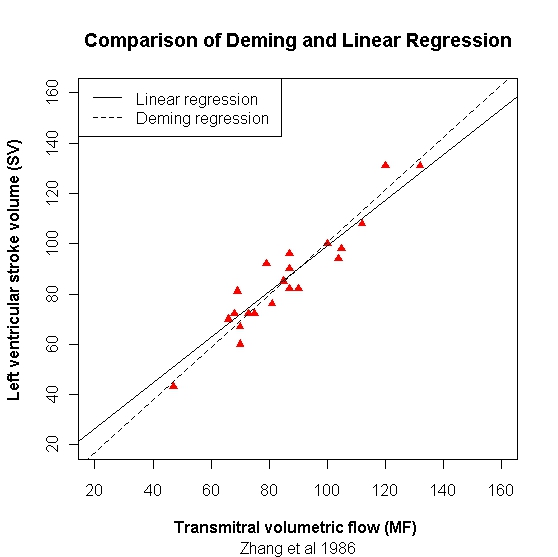
\includegraphics[width=130mm]{images/ZhangDeming.jpeg}
  \caption{Deming Regression For Zhang's Data}\label{ZhangDeming}
\end{figure}


\citet{CarollRupert} states that Deming's
regression is acceptable only when the precision ratio ($\lambda$,
in their paper as $\eta$) is correctly specified, but in practice
this is often not the case, with the $\lambda$ being
underestimated.
\newpage
\section{Other Types of Studies}
\citet{lewis} categorize method comparison studies into three
different types.  The key difference between the first two is
whether or not a `gold standard' method is used. In situations
where one instrument or method is known to be `accurate and
precise', it is considered as the`gold standard' \citep{lewis}. A
method that is not considered to be a gold standard is referred to
as an `approximate method'. In calibration studies they are
referred to a criterion methods and test methods respectively.


\textbf{1. Calibration problems}. The purpose is to establish a
relationship between methods, one of which is an approximate
method, the other a gold standard. The results of the approximate
method can be mapped to a known probability distribution of the
results of the gold standard \citep{lewis}. (In such studies, the
gold standard method and corresponding approximate method are
generally referred to a criterion method and test method
respectively.) \citet*{BA83} make clear that their methodology is
not intended for calibration problems.

\bigskip \textbf{2. Comparison problems}. When two approximate
methods, that use the same units of measurement, are to be
compared. This is the case which the Bland-Altman methodology is
specfically intended for, and therefore it is the most relevant of
the three.

\bigskip \textbf{3. Conversion problems}. When two approximate
methods, that use different units of measurement, are to be
compared. This situation would arise when the measurement methods
use 'different proxies', i.e different mechanisms of measurement.
\citet{lewis} deals specifically with this issue. In the context
of this study, it is the least relevant of the three.

\citet[p.47]{DunnSEME} cautions that`gold standards' should not be
assumed to be error free. `It is of necessity a subjective
decision when we come to decide that a particular method or
instrument can be treated as if it was a gold standard'. The
clinician gold standard , the sphygmomanometer, is used as an
example thereof.  The sphygmomanometer `leaves considerable room
for improvement' \citep{DunnSEME}. \citet{pizzi} similarly
addresses the issue of glod standards, `well-established gold
standard may itself be imprecise or even unreliable'.


The NIST F1 Caesium fountain atomic clock is considered to be the
gold standard when measuring time, and is the primary time and
frequency standard for the United States. The NIST F1 is accurate
to within one second per 60 million years \citep{NIST}.

Measurements of the interior of the human body are, by definition,
invasive medical procedures. The design of method must balance the
need for accuracy of measurement with the well-being of the
patient. This will inevitably lead to the measurement error as
described by \citet{DunnSEME}. The magnetic resonance angiogram,
used to measure internal anatomy,  is considered to the gold
standard for measuring aortic dissection. Medical test based upon
the angiogram is reported to have a false positive reporting rate
of 5\% and a false negative reporting rate of 8\%. This is
reported as sensitivity of 95\% and a specificity of 92\%
\citep{ACR}.

In literature they are, perhaps more accurately, referred to as
`fuzzy gold standards' \citep{phelps}. Consequently when one of the methods is
essentially a fuzzy gold standard, as opposed to a `true' gold
standard, the comparison of the criterion and test methods should
be consider in the context of a comparison study, as well as of a
calibration study.

\newpage


%%%%%%%%%%%%%%%%%%%%%%%%%%%%%%%%%%%%%%%%%%%%%%%%%%%%%%%%%%%%%%%%%%%%%%%%%%%%%%%%%%%%%%%%%%%%%%%%%%%%%%%%%%%%%%%%%%%%%
%%%%%%%%%%%%%%%%%%%%%%%%%%%%%%%%%%%%%%%%%%%%%%%%%%%%%%%%%%%%%%%%%%%%%%%%%%%%%%%%%%%%%%%%%%%%%%%%%%%%%%%%%%%%%%%%%%%%%
	%---------------------------------------------%
	\section{Coefficient of Repeatability}
	\subsection{Repeatability}
	As mentioned previously, \citet{Barnhart} emphasizes the importance of repeatability as part of an overall method comparison study. The coefficient of repeatability was proposed by \citet{BA99}, and is referenced in subsequent papers, such as \citet{BXC2008}. The coefficient of repeatability is a measure of how well a
	measurement method agrees with itself over replicate measurements
	\citep{BA99}. The coefficient of repeatability is a measure of how well a
	measurement method agrees with itself over replicate measurements
	\citep{BA99}. Once the the standard deviations of the differences between the two measurements (in some texts called the residual standard deviation or within-item variability) $sigma_m$ is determined, the
	computation of the coefficients of repeatability for both methods
	is straightforward. The coefficient is calculated from the (in some texts called the residual standard deviation) as  $1.96 \times \sqrt{2} \times \sigma_m$ = $2.83 \sigma_m$).
	
	\subsection{Note 1: Coefficient of Repeatability}
	The coefficient of repeatability is a measure of how well a
	measurement method agrees with itself over replicate measurements
	\citep{BA99}. Once the within-item variability is known, the
	computation of the coefficients of repeatability for both methods
	is straightforward.
	
	
	%------------------------------------------------------------------------------%
	
	\subsection{Repeatability coefficient}
	\citet{BA99} introduces the repeatability coefficient for a method, which is defined as the upper limits of a prediction interval for the absolute difference between two measurements by the same
	method on the same item under identical circumstances \citep{BXC2008}.
	
	$\sigma^2_{x}$ is the within-subject variance of method $x$. The repeatability coefficient is $2.77 \sigma_{x}$ (i.e. $1.96 \times \sqrt{2} \sigma_{x}$). For $95\%$ of subjects, two replicated measurement by the same method will be within this repeatability coefficient.
	
	
	
	\section{Repeatability}
	\subsection{What is Repeatability}
	The quality of repeatability is the ability of a measurement method to give consistent results for a particular subject. That is to say that a measurement will agree with prior and subsequent measurements of the same subject.
	
	\subsection{Repeatability}
	Repeatability (or \textit{test-retest reliability})  describes the variation in measurements taken by a single method of measurement on the same item and under the same conditions. 
	A less-than-perfect test-retest reliability causes test-retest variability. Such variability can be caused by, for example, intra-individual variability and intra-observer variability. 
	A measurement may be said to be repeatable when this variation is smaller than some agreed limit.
	
	Test-retest variability is practically used, for example, in medical monitoring of conditions. In these situations, there is often a predetermined "critical difference", and for differences in monitored values that are smaller than this critical difference, the possibility of pre-test variability as a sole cause of the difference may be considered in addition to, for examples, changes in diseases or treatments.
	
	According to the \textit{Guidelines for Evaluating and Expressing the Uncertainty of NIST Measurement Results}, the following conditions need to be fulfilled in the establishment of repeatability:
	\begin{itemize}
		\item	the same measurement procedure
		\item	the same observer
		\item	the same measuring instrument, used under the same conditions
		\item	the same location
		\item	repetition over a short period of time.
		\item  same objectives
	\end{itemize}
	\bigskip
	
	Repeatability is defined by the \textbf{IUPAC} as `\textit{the closeness of agreement between independent results obtained with the same method on identical test material, under the same conditions (same
		operator, same apparatus, same laboratory and after short intervals of time)}'  and is determined by taking multiple measurements on a series of subjects.
	
	A measurement method can be said to have a good level of repeatability if there is consistency in repeated measurements on the same subject using that method. Conversely, a method has poor repeatability if there is considerable variation in repeated measurements.
	
	
	
	%-----------------------------------------------------------------------------------------------------%
	\newpage
	\section{Importance of Repeatability in MCS}
	
	
	
	Barnhart emphasizes the importance of repeatability as part of an overall method comparison study. Before there can be good agreement between two methods, a method must have good agreement with itself. The coefficient of repeatability , as proposed by Bland \& Altman (1999) is an important feature of both Carstensen's and Roy's methodologies. The coefficient is calculated from the residual standard deviation (i.e. $1.96 \times \sqrt{2} \times \sigma_m$ = $2.83 \sigma_m$).
	
	
	\citet{Barnhart} emphasizes the importance of repeatability as part of an overall method comparison study. Before there can be good agreement between two methods, a method must have good agreement with itself. The coefficient of repeatability , as proposed by \citet{BA99} is an important feature of both Carstensen's and Roy's methodologies. The coefficient is calculated from the residual standard deviation (i.e. $1.96 \times \sqrt{2} \times \sigma_m$ = $2.83 \sigma_m$).
	
	\bigskip
	
	\citet{BA99} strongly recommends the simultaneous estimation of repeatability and agreement be collecting replicated data. \citet{ARoy2009} notes the lack of convenience in such calculations.
	It is important to report repeatability when assessing measurement, because it measures the purest form of random error not influenced by other factors \citep{Barnhart}.	
	
	%% Who Said Next Line
	importance of repeatability' curiously replicate measurements are rarely made in method comparison studies, so that an important aspect of comparability is often overlooked.
	
	Repeatability is important in the context of method comparison because the repeatability of two methods influence the amount of agreement which is possible between those methods. If one method has poor repeatability, the agreement is bound to be poor. If both methods have poor repeatability, agreement is even worse. If one method has poor repeatability in the sense of considerable variability, then agreement between two methods is bound to be poor \citep{ARoy2009}.
	
	\citet{barnhart} and \citet{roy} highlight the importance of reporting repeatability in method comparison, because it measures the purest random error not influenced by any external factors. Statistical procedures on within-subject variances of two methods are equivalent to tests on their respective repeatability coefficients. A formal test is introduced by \citet{roy}, which will discussed in due course.
	
	%--------------------------------------------------------------------%
	%\subsection{Bland and Altman 1999}
	As noted by Bland and Altman 1999, the repeatability of two methods of measurement can  potentially limit
	Repeatability (using Bland-Altman plot)
	The Bland-Altman plot may also be used to assess a method?s repeatability by comparing repeated measurements using one single measurement method on a sample of items.
	The plot can then also be used to check whether the variability or precision of a method is related to the size of the characteristic being measured.
	Since for the repeated measurements the same method is used, the mean difference should be zero.
	Therefore the Coefficient of Repeatability (CR) can be calculated as 1.96 (often rounded to 2) times the standard deviation of the case-wise differences.
	
	\subsection{Coefficient of Repeatability}
	The coefficient of repeatability is a measure of how well a
	measurement method agrees with itself over replicate measurements
	\citep{BA99}. Once the within-item variability is known, the
	computation of the coefficients of repeatability for both methods
	is straightforward.
	
	The British standards Insitute [$1979$] define a coefficient of
	repeatability  as \emph{the value below which the difference between two single test results....may be expected to lie within a specified probability.} Unless otherwise instructed, the
	probability is assumed to be $95\%$. 
	
	The Bland Altman method offers a measurement on the repeatability of the methods. The \emph{Coefficient of Repeatability} (CR) can be calculated as 1.96 (or 2) times the standard deviations of the differences between the two measurements ($d_2$ and $d_1$).
	
	
	
	
	
	%	If one method has poor repeatability in the sense of considerable variability, then agreement between two methods is bound to be poor \citep{ARoy2009}.
	
	
	
	
	
	
	\subsection{Repeatability coefficient from LME Models}
	\citet{BA99} introduces the repeatability coefficient for a method, which is defined as the upper limits of a prediction interval for the absolute difference between two measurements by the same
	method on the same item under identical circumstances \citep{BXC2008}.
	
	$\sigma^2_{x}$ is the within-subject variance of method $x$. The repeatability coefficient is $2.77 \sigma_{x}$ (i.e. $1.96 \times \sqrt{2} \sigma_{x}$). For $95\%$ of subjects, two replicated measurement by the same method will be within this repeatability coefficient.
	
	%% \section{Note 1: Coefficient of Repeatability}
	
	
	
	%------------------------------------------------------------------------------------------%
	\subsection{Repeatability in Bland-Altman Blood Data Analysis}
	\begin{itemize}
		\item Two readings by the same method will be within $1.96
		\sqrt{2} \sigma_w $ or $2.77 \sigma_w $ for 95\% of subjects. Thisvalue is called the repeatability coefficient.
		
		\item For observer J using the sphygmomanometer $ \sigma_w = \sqrt{37.408} = 6.116$ and so the repeatability coefficient is
		$2:77 \times 6.116 = 16:95$ mmHg.
		
		\item For the machine S,$ \sigma_w = \sqrt{83.141} = 9.118$ and the repeatability coefficient is $2:77 \times 9.118 = 25.27$ mmHg.
		
		\item Thus, the repeatability of the machine is 50\% greater than that of the observer.
	\end{itemize}
	%-------------------------------------------------------------------%
	\section{Carstensen}
	\begin{itemize}
		\item The limits of agreement are not always the only issue of
		interest � the assessment of method specific repeatability and
		reproducibility are of interest in their own right.
		
		\item Repeatability can only be assessed when replicate
		measurements by each method are available.
		
		\item The repeatability coefficient for a method is defined as the
		upper limits of a prediction interval for the absolute difference
		between two measurements by the same method on the same item under
		identical circumstances.
		
		\item If the standard deviation of a measurement is $\sigma$ the
		repeatability coefficient is $2\times\sqrt{2} \sigma = 2.83\times
		\sigma \approx 2.8 \sigma$.
		
		
		\item The repeatability of measurement methods is calculated
		differently under the two models \item Under the model assuming
		exchangeable replicates (1), the repeatability is based only on
		the residual standard deviation, i.e. $2.8\sigma_m$
		
		
		\item Under the model for linked replicates (2) there are two
		possibilities depending on the circumstances.
		
		\item If the variation between replicates within item can be
		considered a part of the repeatability it will be $2.8 \sqrt{
			\omega^2 + \sigma^2_m}$.
		
		\item However, if replicates are taken under substantially
		different circumstances, the variance component $\omega^2$ may be
		considered irrelevant in the repeatability and one would therefore
		base the repeatability on the measurement errors alone, i.e. use
		$2.8 \sigma_m$.
	\end{itemize}
	
	
	
	%\section{Reproducibility}
	% 
	%It is advisable to be able to distinguish between Repeatability and a similar concept ?Reproducibility?. Reproducibility is
	
	
	
	
	
	
	
	
	
	%%========================================================================%
	%% Phase Next Section Out
	%% Where did this come from
	
	\newpage
	
	%--------------------------------------------------------------------%
	
	%--------------------------------------------------------------------%
	\subsection{Notes from BXC Book (chapter 9)}
	The assessment of method-specific repeatability and reproducibility is of interest in its own right.
	Repeatability and reproducibility can only be assessed when replicate measurements by each method are available.
	If replicate measurements by a method are available, it is simple to estimate the measurement error for a method, using a model with fixed effects for item, then taking the residual standard deviation as measurement error standard deviation.
	However, if replicates are linked, this may produce an estimate that biased upwards.
	The repeatability coefficient (or simply repeatability) for a method is defined as the upper limit of a
	prediction interval for the absolute difference between two measurements by the same method on the same
	item under identical circumstances (see above conditions)
	
	\[y_{mir}  = \alpha_{m} + \beta_m( \mu_i + a_{ir} + c_{mi}) + e_{mir}\]
	
	The variation between measurements under identical circumstances.

\chapter{Linear Mixed effects Models}
\section{Linear Mixed effects Models}
A linear mixed effects (LME) model is a statistical model containing both fixed effects and random effects (random effects are also known as variance components). LME models are a generalization of the classical linear model, which contain fixed effects only. When the levels of factors are considered to be sampled from a population,
and each level is not of particular interest, they are considered random quantities with associated variances.
The effects of the levels, as described, are known as random effects. Random effects are represented by unobservable
normally distributed random variables. Conversely fixed effects are considered non-random and the
levels of each factor are of specific interest.
%LME models are useful models when considering repeated measurements or grouped observations.

\citet{Fisher4} introduced variance components models for use in genetical studies. Whereas an estimate for variance must take an non-negative value, an individual variance component, i.e.\ a component of the overall variance, may be negative.

The framework has developed since, including contributions from
\citet{tippett}, who extend the use of variance components into linear models, and \citet{eisenhart}, who introduced the `mixed model' terminology and formally distinguished between mixed and random effects models. \citet{Henderson:1950} devised a framework for deriving estimates for both the fixed effects and the random effects, using a set of equations that would become known as `mixed model equations' or `Henderson's equations'.
LME methodology is further enhanced by Henderson's later works \citep{Henderson53, Henderson59,Henderson63,Henderson73,Henderson84a}. The key features of Henderson's work provide the basis for the estimation techniques.

\citet{HartleyRao} demonstrated that unique estimates of the variance components could be obtained using maximum likelihood methods. However these estimates are known to be biased `downwards' (i.e.\ underestimated) , because of the assumption that the fixed estimates are known, rather than being estimated from the data. \citet{PattersonThompson} produced an alternative set of estimates, known as the restricted maximum likelihood (REML) estimates, that do not require the fixed effects to be known. Thusly there is a distinction the REML estimates and the original estimates, now commonly referred to as ML estimates.

\citet{LW82} provides a form of notation for notation for LME models that has since become the standard form, or the basis for more complex formulations. Due to computation complexity, linear mixed effects models have not seen widespread use until many well known statistical software applications began facilitating them. SAS Institute added PROC MIXED to its software suite in 1992 \citep{singer}. \citet{PB} described how to compute LME models in the \texttt{S-plus} environment.

Using Laird-Ware form, the LME model is commonly described in matrix form,
\begin{equation}
y = X\beta + Zb + \epsilon
\label{LW}
\end{equation}

\noindent where $y$ is a vector of $N$ observable random variables, $\beta$ is a vector of $p$ fixed effects, $X$ and $Z$ are $N \times p$ and $N \times q$ known matrices, and $b$ and $\epsilon$  are vectors of $q$ and $N,$ respectively, random effects such that $\mathrm{E}(b)=0, \ \mathrm{E}(\epsilon)=0$
and
\[
\mathrm{var}
\left(
              \begin{array}{c}
                b \\
                \epsilon \\
              \end{array}
            \right)
   =
\left(
         \begin{array}{cc}
           D & 0 \\
           0 & \Sigma \\
         \end{array}
       \right)
\]




where $D$ and $\Sigma$ are positive definite matrices parameterized by an unknown variance component parameter vector $ \theta.$ The variance-covariance matrix for the vector of observations $y$ is given by $V = ZDZ^{\prime}+ \Sigma.$ This implies $y \sim(X\beta, V) = (X\beta,ZDZ^{\prime}+ \Sigma)$. It is worth noting that $V$ is an $n \times n$ matrix, as the dimensionality becomes relevant later on. The notation provided here is generic, and will be adapted to accord with complex formulations that will be encountered in due course.

%\subsection{Likelihood and estimation}

% Likelihood is the hypothetical probability that an event that has already occurred would yield a specific outcome. Likelihood differs from probability in that probability refers to future occurrences, while likelihood refers to past known outcomes.

% The likelihood function ($L(\theta)$)is a fundamental concept in statistical inference. It indicates how likely a particular population is to produce an observed sample. The set of values that maximize the likelihood function are considered to be optimal, and are used as the estimates of the parameters. For computational ease, it is common to use the logarithm of the likelihood function, known simply as the log-likelihood ($\ell(\theta)$).


\subsection{Estimation}
Estimation of LME models involve two complementary estimation issues'; estimating the vectors of the fixed and random effects estimates $\hat{\beta}$ and $\hat{b}$ and estimating the variance covariance matrices $D$ and $\Sigma$.
Inference about fixed effects have become known as `estimates', while inferences about random effects have become known as `predictions'. The most common approach to obtain estimators are Best Linear Unbiased Estimator (BLUE) and Best Linear Unbiased Predictor (BLUP). For an LME model given by (\ref{LW}), the BLUE of $\hat{\beta}$ is given by
\[\hat{\beta} = (X^\prime V^{-1}X)^{-1}X^\prime V^{-1}y,\]whereas the BLUP of $\hat{b}$ is given by
\[\hat{b} = DZ^{\prime} V^{-1} (y-X\hat{\beta}).\]

\subsubsection{Henderson's equations}
Because of the dimensionality of V (i.e. $n \times n$) computing the inverse of V can be difficult. As a way around the this problem \citet{Henderson53, Henderson59,Henderson63,Henderson73,Henderson84a} offered a more simpler approach of jointly estimating $\hat{\beta}$ and $\hat{b}$.
\cite{Henderson:1950} made the (ad-hoc) distributional assumptions $y|b \sim \mathrm{N} (X \beta + Zb, \Sigma)$ and $b \sim \mathrm{N}(0,D),$ and proceeded to maximize the joint density of $y$ and $b$
\begin{equation}
\left|
\begin{array}{cc}
D & 0 \\
0 & \Sigma \\
\end{array}
  \right|^{-\frac{1}{2}}
\exp
\left\{ -\frac{1}{2}
\left(
\begin{array}{c}
                b \\
                y - X \beta -Zb \\
              \end{array}
            \right)^\prime
\left( \begin{array}{cc}
D & 0 \\
0 & \Sigma \\
\end{array}\right)^{-1}
\left(
\begin{array}{c}
                b \\
                y - X \beta -Zb \\
              \end{array}
            \right)
\right\},
\label{u&beta:JointDensity}
\end{equation}
with respect to $\beta$ and $b,$ which ultimately requires minimizing the criterion
\begin{equation}
(y - X \beta -Zb)'\Sigma^{-1}(y - X \beta -Zb) + b^\prime D^{-1}b.
\label{Henderson:Criterion}
\end{equation}
This leads to the mixed model equations
\begin{equation}
\left(\begin{array}{cc}
  X^\prime\Sigma^{-1}X & X^\prime\Sigma^{-1}Z
  \\
  Z^\prime\Sigma^{-1}X & X^\prime\Sigma^{-1}X + D^{-1}
  \end{array}\right)
\left(\begin{array}{c}
    \beta \\
  b
  \end{array}\right)
  =
\left(\begin{array}{c}
  X^\prime\Sigma^{-1}y \\
  Z^\prime\Sigma^{-1}y
  \end{array}\right).
\label{Henderson:Equations}
\end{equation}
Using these equations, obtaining the estimates requires the inversion of a matrix
of dimension $p+q \times p+q$, considerably smaller in size than $V$. \citet{Henderson1963} shows that these mixed model equations do not depend on normality and that $\hat{\beta}$ and $\hat{b}$ are the BLUE and BLUP under general conditions, provided $D$ and $\Sigma$ are known.

\cite{Robi:BLUP:1991} points out that although \cite{Henderson:1950} initially referred to the estimates $\hat{\beta}$ and $\hat{b}$ from (\ref{Henderson:Equations}) as ``joint maximum likelihood estimates", \cite{Henderson:1973} later advised that these estimates should not be referred to as ``maximum likelihood" as the function being maximized in (\ref{Henderson:Criterion}) is a joint density rather than a likelihood function. \cite{Lee:Neld:Pawi:2006} remarks that it is clear that Henderson used joint estimation for computational purposes, without recognizing the theoretical implications.

\subsubsection{Estimation of the fixed parameters}

The vector $y$ has marginal density $y \sim \mathrm{N}(X \beta,V),$ where $V = \Sigma + ZDZ^\prime$ is specified through the variance component parameters $\theta.$ The log-likelihood of the fixed parameters $(\beta, \theta)$ is
\begin{equation}
\ell (\beta, \theta|y) =
-\frac{1}{2} \log |V| -\frac{1}{2}(y -
X \beta)'V^{-1}(y -
X \beta), \label{Likelihood:MarginalModel}
\end{equation}
and for fixed $\theta$ the estimate $\hat{\beta}$ of $\beta$ is obtained as the solution of
\begin{equation}
(X^\prime V^{-1}X) {\beta} = X^\prime V^{-1}y.
\label{mle:beta:hat}
\end{equation}

Substituting $\hat{\beta}$ from (\ref{mle:beta:hat}) into $\ell(\beta, \theta|y)$ from (\ref{Likelihood:MarginalModel}) returns the \emph{profile} log-likelihood
\begin{eqnarray*}
\ell_P(\theta \mid y) &=& \ell(\hat{\beta}, \theta \mid y) \\
&=& -\frac{1}{2} \log |V| -\frac{1}{2}(y - X \hat{\beta})'V^{-1}(y - X \hat{\beta})
\end{eqnarray*}
of the variance parameter $\theta.$ Estimates of the parameters $\theta$ specifying $V$ can be found by maximizing $\ell_P(\theta \mid y)$ over $\theta.$ These are the ML estimates.

For REML estimation the \emph{restricted} log-likelihood is defined as
\[
\ell_R(\theta \mid y) =
\ell_P(\theta \mid y) -\frac{1}{2} \log |X^\prime VX |.
\]
%\subsubsection{Likelihood estimation techniques}
%Maximum likelihood and restricted maximum likelihood have become the most common strategies
%for estimating the variance component parameter $\theta.$ Maximum likelihood estimation obtains
%parameter estimates by optimizing the likelihood function.
%To obtain ML estimate the likelihood is constructed as a function of the parameters in the specified LME model.
% The maximum likelihood estimates (MLEs) of the parameters are the values of the arguments that maximize the likelihood function.

The REML approach does not base estimates on a maximum likelihood fit of all the information, but instead uses a likelihood function derived from a data set, transformed to remove the irrelevant influences \citep{REMLDefine}.
Restricted maximum likelihood is often preferred to maximum likelihood because REML estimation reduces the bias in the variance component by taking into account the loss of degrees of freedom that results
from estimating the fixed effects in $\boldsymbol{\beta}$. Restricted maximum likelihood also handles high correlations more effectively, and is less sensitive to outliers than maximum likelihood.  The problem with REML for model building is that the likelihoods obtained for different fixed effects are not comparable. Hence it is not valid to compare models with different fixed effects using a likelihood ratio test or AIC when REML is used to
estimate the model. Therefore models derived using ML must be used instead.

\subsubsection{Estimation of the random effects}

The established approach for estimating the random effects is to use the best linear predictor of $b$ from $y,$ which for a given $\beta$ equals $DZ^\prime V^{-1}(y - X \beta).$ In practice $\beta$ is replaced by an estimator such as $\hat{\beta}$ from (\ref{mle:beta:hat}) so that $\hat{b} = DZ^\prime V^{-1}(y - X \hat{\beta}).$ Pre-multiplying by the appropriate matrices it is straightforward to show that these estimates $\hat{\beta}$ and $\hat{b}$ satisfy the equations in (\ref{Henderson:Equations}).

\subsubsection{Algorithms for likelihood function optimization}Iterative numerical techniques are used to optimize the log-likelihood function and estimate the covariance parameters $\theta$. The procedure is subject to the constraint that $R$ and $D$ are both positive definite. The most common iterative algorithms for optimizing the likelihood function are the Newton-Raphson method, which is the preferred method, the expectation maximization (EM) algorithm and the Fisher scoring methods.

The EM algorithm, introduced by \citet{EM}, is an iterative technique for maximizing complicated likelihood functions. The algorithm alternates between performing an expectation (E) step
and the maximization (M) step. The `E' step computes the expectation of the log-likelihood evaluated using the current
estimate for the variables. In the `M' step, parameters that maximize the expected log-likelihood, found on the previous `E' step, are computed. These parameter estimates are then used to determine the distribution of the variables in the next `E' step. The algorithm alternatives between these two steps until convergence is reached.

The main drawback of the EM algorithm is its slow rate of
convergence. Consequently the EM algorithm is rarely used entirely in LME estimation,
instead providing an initial set of values that can be passed to
other optimization techniques.

The Newton Raphson (NR) method is the most common, and recommended technique for ML and
REML estimation. The NR algorithm minimizes an objective function defines as $-2$ times the log likelihood for the covariance parameters $\theta$. At every iteration the NR algorithm requires the
calculation of a vector of partial derivatives, known as the gradient, and the second derivative matrix with respect to the covariance parameters. This is known as the observed Hessian matrix. Due to the Hessian matrix, the NR algorithm is more time-consuming, but convergence is reached with fewer iterations compared to the EM algorithm. The Fisher scoring algorithm is an variant of the NR algorithm that is more numerically stable and likely to converge, but not recommended to obtain final estimates.

\subsubsection{The extended likelihood}

The desire to have an entirely likelihood-based justification for estimates of random effects, in contrast to Henderson's equation, has motivated \citet[page 429]{Pawi:in:2001} to define the \emph{extended likelihood}. He remarks ``In mixed effects modelling the extended likelihood has been called \emph{h-likelihood} (for hierarchical  likelihood) by \cite{Lee:Neld:hier:1996}, while in smoothing literature it is known as the \emph{penalized likelihood} (e.g.\ \citeauthor{Gree:Silv:nonp:1994} \citeyear{Gree:Silv:nonp:1994})." The extended likelihood can be written $L(\beta,\theta,b|y) = p(y|b;\beta,\theta) p(b;\theta)$ and adopting the same distributional assumptions used by \cite{Henderson:1950} yields the log-likelihood function

\begin{eqnarray*}
\ell_h(\beta,\theta,b|y)
& = \displaystyle -\frac{1}{2} \left\{ \log|\Sigma| + (y - X \beta -Zb)'\Sigma^{-1}( y - X \beta -Zb) \right.\\
&  \hspace{0.5in} \left. + \log|D| + b^\prime D^{-1}b \right\}.
\end{eqnarray*}
Given $\theta$, differentiating with respect to $\beta$ and $b$ returns Henderson's equations in (\ref{Henderson:Equations}).

\subsubsection{The LME model as a general linear model}
Henderson's equations in (\ref{Henderson:Equations}) can be rewritten $( T^\prime W^{-1} T ) \delta = T^\prime W^{-1} y_{a} $ using
\[
\delta = \left(\begin{array}{c}\beta \\ b \end{array}\right),
\ y_{a} = \left(\begin{array}{c}
  y \cr \psi
  \end{array}\right),
\ T = \left(\begin{array}{cc}
  X & Z  \\
  0 & I
  \end{array}\right),
\ \textrm{and} \ W = \left(\begin{array}{cc}
  \Sigma & 0  \cr
  0 &  D \end{array}\right),
\]
where \cite{Lee:Neld:Pawi:2006} describe $\psi = 0$ as quasi-data with mean $\mathrm{E}(\psi) = b.$ Their formulation suggests that the joint estimation of the coefficients $\beta$ and $b$ of the linear mixed effects model can be derived via a classical augmented general linear model $y_{a} = T\delta + \varepsilon$ where $\mathrm{E}(\varepsilon) = 0$ and $\mathrm{var}(\varepsilon) = W,$ with \emph{both} $\beta$ and $b$ appearing as fixed parameters. The usefulness of this reformulation of an LME as a general linear model will be revisited.


%------------------------------------------------------------------------------------%
\newpage                                                                    % - Section 4
%----------------------------------------------------------------------------------------%
\section{Repeated Measurements in LME models}

In many statistical analyzes, the need to determine parameter estimates where multiple measurements are available on each of a set of variables often arises. Further to \citet{lam}, \citet{hamlett} performs an analysis of the correlation of replicate measurements, for two variables of interest, using LME models.

Let $y_{Aij}$ and $y_{Bij}$ be the $j$th repeated observations of the variables of interest $A$ and $B$ taken on the $i$th subject. The number of repeated measurements for each variable may differ for each individual.
Both variables are measured on each time points. Let $n_{i}$ be the number of observations for each variable, hence $2\times n_{i}$ observations in total.

It is assumed that the pair $y_{Aij}$ and $y_{Bij}$ follow a bivariate normal distribution.
\begin{eqnarray*}
\left(
  \begin{array}{c}
    y_{Aij} \\
    y_{Bij} \\
  \end{array}
\right) \sim \mathcal{N}(
    \boldsymbol{\mu}, \boldsymbol{\Sigma})\mbox{   where } \boldsymbol{\mu} = \left(
  \begin{array}{c}
    \mu_{A} \\
    \mu_{B} \\
  \end{array}
\right)
\end{eqnarray*}

The matrix $\Sigma$ represents the variance component matrix between response variables at a given time point $j$.

\[
\boldsymbol{\Sigma} = \left( \begin{array}{cc}
                        \sigma^2_{A} & \sigma_{AB} \\
                        \sigma_{AB} & \sigma^2_{B}\\
                      \end{array}   \right)
\]

$\sigma^2_{A}$ is the variance of variable $A$, $\sigma^2_{B}$ is the variance of variable $B$ and $\sigma_{AB}$ is the covariance of the two variable. It is assumed that $\boldsymbol{\Sigma}$ does not depend on a particular time point, and is the same over all time points.

%------------------------------------------------------------------------------%
\subsection{Formulation of the Response Vector}
 Information of individual $i$ is recorded in a response vector $\boldsymbol{y}_{i}$. The response vector is constructed by stacking the response of the $2$ responses at the first instance, then the $2$ responses at the second instance, and so on. Therefore the response vector is a $2n_{i} \times 1$ column vector.
The covariance matrix of $\boldsymbol{y_{i}}$ is a $2n_{i} \times 2n_{i}$ positive definite matrix $\boldsymbol{\Omega}_{i}$.

Consider the case where three measurements are taken by both methods $A$ and $B$, $\boldsymbol{y}_{i}$ is a $6 \times 1$ random vector describing the $i$th subject.
\[
\boldsymbol{y}_{i} = (y_{i}^{A1},y_{i}^{B1},y_{i}^{A2},y_{i}^{B2},y_{i}^{A3},y_{i}^{B3}) \prime
\]

The response vector $\boldsymbol{y_{i}}$ can be formulated as an LME model according to Laird-Ware form.
\begin{eqnarray*}
\boldsymbol{y_{i}} = \boldsymbol{X_{i}\beta}  + \boldsymbol{Z_{i}b_{i}} + \boldsymbol{\epsilon_{i}}\\
\boldsymbol{b_{i}} \sim \mathcal{N}(\boldsymbol{0,D})\\
\boldsymbol{\epsilon_{i}} \sim \mathcal{N}(\boldsymbol{0,R_{i}})
\end{eqnarray*}

Information on the fixed effects are contained in a three dimensional vector $\boldsymbol{\beta} = (\beta_{0},\beta_{1},\beta_{2})\prime$. For computational purposes $\beta_{2}$ is conventionally set to zero. Consequently $\boldsymbol{\beta}$ is the solutions of the means of the two methods, i.e. $E(\boldsymbol{y}_{i})  = \boldsymbol{X}_{i}\boldsymbol{\beta}$. The variance covariance matrix $\boldsymbol{D}$ is a general $2 \times 2$ matrix, while $\boldsymbol{R}_{i}$ is a $2n_{i} \times 2n_{i}$ matrix.

%------------------------------------------------------------------------------%
\subsection{Decomposition of the response covariance matrix}

The variance covariance structure can be re-expressed in the following form,
\[
\mbox{Cov}(\mbox{y}_{i}) = \boldsymbol{\Omega_{i}} = \boldsymbol{Z}_{i}\boldsymbol{D}\boldsymbol{Z}_{i}^\prime + \boldsymbol{R_{i}}.
\]

$\boldsymbol{R_{i}}$ can be shown to be the Kronecker product of a correlation matrix $\boldsymbol{V}$ and $\boldsymbol{\Lambda}$. The correlation matrix $\boldsymbol{V}$ of the repeated measures on a given response variable is assumed to be the same for all response variables. Both \citet{hamlett} and \citet{lam} use the identity matrix, with dimensions $n_{i} \times n_{i}$ as the formulation for $\boldsymbol{V}$. \citet{roy} remarks that, with repeated measures, the response for each subject is correlated for each variable, and that such correlation must be taken into account in order to produce a valid inference on correlation estimates.  \citet{roy2006} proposes various correlation structures may be assumed for repeated measure correlations, such as the compound symmetry and autoregressive structures, as alternative to the identity matrix.

However, for the purposes of method comparison studies, the necessary estimates are currently only determinable when the identity matrix is specified, and the results in \citet{roy} indicate its use.

For the response vector described, \citet{hamlett} presents a detailed covariance matrix. A brief summary shall be presented here only. The overall variance matrix is a $6 \times 6$ matrix composed of two types of $2 \times 2$ blocks. Each block represents one separate time of measurement.

\[
\boldsymbol{\Omega}_{i} = \left(
\begin{array}{ccc}
  \boldsymbol{\Sigma} & \boldsymbol{D} & \boldsymbol{D}\\
  \boldsymbol{D} & \boldsymbol{\Sigma} & \boldsymbol{D}\\
  \boldsymbol{D} & \boldsymbol{D} & \boldsymbol{\Sigma}\\
\end{array}\right)
\]

The diagonal blocks are $\Sigma$, as described previously. The $2 \times 2$ block diagonal matrix in $\boldsymbol{\Omega}$ gives $\boldsymbol{\Sigma}$. $\boldsymbol{\Sigma}$ is the sum of the between-subject variability $\boldsymbol{D}$ and the within subject variability $\boldsymbol{\Lambda}$.

$\boldsymbol{\Omega_{i}}$ can be expressed as
\[
\boldsymbol{\Omega_{i}} = \boldsymbol{Z}_{i}\boldsymbol{D}\boldsymbol{Z}_{i}^\prime + ({\boldsymbol{I_{n_{i}}} \otimes \boldsymbol{\Lambda}}).
\]
The notation $\mbox{dim}_{n_{i}}$ means an $n_{i} \times n_{i}$ diagonal block.

\subsection{Correlation terms}
\citet{hamlett} demonstrated how the between-subject and within subject variabilities can be expressed in terms of
correlation terms.

\[
\boldsymbol{D} = \left( \begin{array}{cc}
                        \sigma^2_{A}\rho_{A} & \sigma_{A}\sigma_{b}\rho_{AB}\delta \\
                        \sigma_{A}\sigma_{b}\rho_{AB}\delta & \sigma^2_{B}\rho_{B}\\

                      \end{array}\right)
\]

\[
\boldsymbol{\Lambda} = \left(
\begin{array}{cc}
  \sigma^2_{A}(1-\rho_{A}) & \sigma_{AB}(1-\delta)  \\
    \sigma_{AB}(1-\delta) & \sigma^2_{B}(1-\rho_{B}) \\
\end{array}\right).
\]

$\rho_{A}$ describe the correlations of measurements made by the method $A$ at different times. Similarly $\rho_{B}$ describe the correlation of measurements made by the method $B$ at different times. Correlations among repeated measures within the same method are known as intra-class correlation coefficients. $\rho_{AB}$ describes the correlation of measurements taken at the same same time by both methods. The coefficient $\delta$ is added for when the measurements are taken at different times, and is a constant of less than $1$ for linked replicates. This is based on the assumption that linked replicates measurements taken at the same time would have greater correlation than those taken at different times. For unlinked replicates $\delta$ is simply $1$. \citet{hamlett} provides a useful graphical depiction of the role of each correlation coefficients.

\newpage
\section{Using LME for method comparison}
Due to the prevalence of modern statistical software, \citet{BXC2008} advocates the adoption of computer based approaches, such as LME models, to method comparison studies. \citet{BXC2008} remarks upon `by-hand' approaches advocated in \citet{BA99} discouragingly, describing them as tedious, unnecessary and `outdated'. Rather than using the `by hand' methods, estimates for required LME parameters can be read directly from program output. Furthermore, using computer approaches removes constraints associated with `by-hand' approaches, such as the need for the design to be perfectly balanced.

\subsection{Roy's Approach}

For the purposes of comparing two methods of measurement, \citet{roy} presents a framework that utilizes linear mixed effects model. This methodology provides for the formal testing of inter-method bias, between-subject variability and within-subject variability of two methods. The formulation contains a Kronecker product covariance structure in a doubly multivariate setup. By doubly multivariate set up, Roy means that the information on each patient or item is multivariate at two levels, the number of methods and number of replicated measurements. Further to \citet{lam}, it is assumed that the replicates are linked over time. However it is easy to modify to the unlinked case.

\citet{roy} sets out three criteria for two methods to be considered in agreement. Firstly that there be no significant bias. Second that there is no difference in the between-subject variabilities, and lastly that there is no significant difference in the within-subject variabilities. Roy further proposes examination of the the overall variability by considering the second and third criteria be examined jointly. Should both the second and third criteria be fulfilled, then the overall variabilities of both methods would be equal.

A formal test for inter-method bias can be implemented by examining the fixed effects of the model. This is common to well known classical linear model methodologies. The null hypotheses, that both methods have the same mean, which is tested against the alternative hypothesis, that both methods have different means.
The inter-method bias and necessary $t-$value and $p-$value are presented in computer output. A decision on whether the first of Roy's criteria is fulfilled can be based on these values.

Importantly \citet{roy} further proposes a series of three tests on the variance components of an LME model, which allow decisions on the second and third of Roy's criteria. For these tests, four candidate LME models are constructed. The differences in the models are specifically in how the the $D$ and $\Lambda$ matrices are constructed, using either an unstructured form or a compound symmetry form. To illustrate these differences, consider a generic matrix $A$,

\[
\boldsymbol{A} = \left( \begin{array}{cc}
    a_{11} & a_{12}  \\
    a_{21} & a_{22}  \\
    \end{array}\right).
\]

A symmetric matrix allows the diagonal terms $a_{11}$ and $a_{22}$ to differ. The compound symmetry structure requires that both of these terms be equal, i.e $a_{11} = a_{22}$.

The first model acts as an alternative hypothesis to be compared against each of three other models, acting as null hypothesis models, successively. The models are compared using the likelihood ratio test. Likelihood ratio tests are a class of tests based on the comparison of the values of the likelihood functions of two candidate models. 






\subsection{Correlation}
In addition to the variability tests, Roy advises that it is preferable that a correlation of greater than $0.82$ exist for two methods to be considered interchangeable. However if two methods fulfil all the other conditions for agreement, failure to comply with this one can be overlooked. Indeed Roy demonstrates that placing undue importance to it can lead to incorrect conclusions. \citet{roy} remarks that current computer implementations only gives overall correlation coefficients, but not their variances. Consequently it is not possible to carry out inferences based on all overall correlation coefficients.

%--------------------------------------------------%
\subsection{Variability test 1}
The first test determines whether or not both methods $A$ and $B$ have the same between-subject variability, further to the second of Roy's criteria.
\begin{eqnarray*}
H_{0}: \mbox{ }d_{A}  = d_{B} \\
H_{A}: \mbox{ }d_{A}  \neq d_{B}
\end{eqnarray*}
This test is facilitated by constructing a model specifying a symmetric form for $D$ (i.e. the alternative model) and comparing it with a model that has compound symmetric form for $D$ (i.e. the null model). For this test $\boldsymbol{\hat{\Lambda}}$ has a symmetric form for both models, and will be the same for both.

%---------------------------------------------%
\subsection{Variability test 2}

This test determines whether or not both methods $A$ and $B$ have the same within-subject variability, thus enabling a decision on the third of Roy's criteria.

\begin{eqnarray*}
H_{0}: \mbox{ }\lambda_{A}  = \lambda_{B} \\
H_{A}: \mbox{ }\lambda_{A}  = \lambda_{B}
\end{eqnarray*}

This model is performed in the same manner as the first test, only reversing the roles of $\boldsymbol{\hat{D}}$ and $\boldsymbol{\hat{\Lambda}}$. The null model is constructed a symmetric form for $\boldsymbol{\hat{\Lambda}}$ while the alternative model uses a compound symmetry form. This time $\boldsymbol{\hat{D}}$ has a symmetric form for both models, and will be the same for both.

As the within-subject variabilities are fundamental to the coefficient of repeatability, this variability test likelihood ratio test is equivalent to testing the equality of two coefficients of repeatability of two methods. In presenting the results of this test, \citet{roy} includes the coefficients of repeatability for both methods.

%-----------------------------------------------%
\subsection{Variability test 3}
The last of the variability test examines whether or not methods $A$ and $B$ have the same overall variability. This enables the joint consideration of second and third criteria.
\begin{eqnarray*}
H_{0}: \mbox{ }\sigma_{A}  = \sigma_{B} \\
H_{A}: \mbox{ }\sigma_{A}  = \sigma_{B}
\end{eqnarray*}

The null model is constructed a symmetric form for both $\boldsymbol{\hat{D}}$ and $\boldsymbol{\hat{\Lambda}}$ while the alternative model uses a compound symmetry form for both.

\subsection{Demonstration of Roy's testing}
Roy provides three case studies, using data sets well known in method comparison studies, to demonstrate how the methodology should be used. The first two examples used are from the `blood pressure' data set introduced by \citet{BA99}. The data set is a tabulation of simultaneous measurements of systolic blood pressure were made by each of two experienced observers (denoted `J' and `R') using a sphygmomanometer and by a semi-automatic blood pressure monitor (denoted `S'). Three sets of readings were made in quick succession. Roy compares the `J' and `S' methods in the first of her examples.

The inter-method bias between the two method is found to be $15.62$ , with a $t-$value of $-7.64$, with a $p-$value of less than $0.0001$. Consequently there is a significant inter-method bias present between methods $J$ and $S$, and the first of the Roy's three agreement criteria is unfulfilled.

Next, the first variability test is carried out, yielding maximum likelihood estimates of the between-subject variance covariance matrix, for both the null model, in compound symmetry (CS) form, and the alternative model in symmetric (symm) form. These matrices are determined to be as follows;
\[
\boldsymbol{\hat{D}}_{CS} = \left( \begin{array}{cc}
    946.50 & 784.32  \\
    784.32 & 946.50  \\
    \end{array}\right),
\hspace{1.5cm}
    \boldsymbol{\hat{D}}_{Symm} = \left( \begin{array}{cc}
    923.98 & 785.24  \\
    785.24 & 971.30  \\
    \end{array}\right).
\]

A likelihood ratio test is perform to compare both candidate models. The log-likelihood of the null model is $-2030.7$, and for the alternative model $-2030.8$. The test statistic, presented with greater precision than the log-likelihoods, is $0.1592$. The $p-$value is $0.6958$. Consequently we fail to reject the null model, and by extension, conclude that the hypothesis that methods $J$ and $S$ have the same between-subject variability. Thus the second of the criteria is fulfilled.

The second variability test determines maximum likelihood estimates of the within-subject variance covariance matrix, for both the null model, in CS form, and the alternative model in symmetric form.

\[
\boldsymbol{\hat{\Lambda}_{CS}} = \left( \begin{array}{cc}
    60.27  & 16.06  \\
    16.06  & 60.27  \\
    \end{array}\right),
\hspace{1.5cm}
\boldsymbol{\hat{\Lambda}}_{Symm} = \left( \begin{array}{cc}
    37.40 & 16.06  \\
    16.06 & 83.14  \\
    \end{array}\right).
\]

Again, A likelihood ratio test is perform to compare both candidate models. The log-likelihood of the alternative model model is $-2045.0$. As before, the null model has a log-likelihood of $-2030.7$. The test statistic is computed as $28.617$, again presented with greater precision. The $p-$value is less than $0.0001$. In this case we reject the null hypothesis of equal within-subject variability. Consequently the third of Roy's criteria is unfulfilled.
The coefficient of repeatability for methods $J$ and $S$ are found to be 16.95 mmHg and 25.28 mmHg respectively.

The last of the three variability tests is carried out to compare the overall variabilities of both methods.
With the null model the MLE of the within-subject variance covariance matrix is given below. The overall variabilities for the null and alternative models, respectively, are determined to be as follows;
\[
\boldsymbol{\hat{\Sigma}}_{CS} = \left( \begin{array}{cc}
    1007.92  & 801.65  \\
    801.65  & 1007.92  \\
    \end{array}\right),
    \hspace{1.5cm}
\boldsymbol{\hat{\Sigma}}_{Symm} = \left( \begin{array}{cc}
    961.38 & 801.40  \\
    801.40 & 1054.43  \\
    \end{array}\right),
\]

The log-likelihood of the alternative model model is $-2045.2$, and again, the null model has a log-likelihood of $-2030.7$. The test statistic is $28.884$, and the $p-$value is less than $0.0001$. The null hypothesis, that both methods have equal overall variability, is rejected. Further to the second variability test, it is known that this difference is specifically due to the difference of within-subject variabilities.

Lastly, Roy considers the overall correlation coefficient. The diagonal blocks $\boldsymbol{\hat{r}_{\Omega}}_{ii}$ of the correlation matrix indicate an overall coefficient of $0.7959$. This is less than the threshold of 0.82 that Roy recommends.

\[
\boldsymbol{\hat{r}_{\Omega}}_{ii} = \left( \begin{array}{cc}
    1  & 0.7959  \\
    0.7959  & 1  \\
    \end{array}\right)
\]

The off-diagonal blocks of the overall correlation matrix $\boldsymbol{\hat{r}_{\Omega}}_{ii'}$ present the correlation coefficients further to \citet{hamlett}.
\[
\boldsymbol{\hat{r}_{\Omega}}_{ii'} = \left( \begin{array}{cc}
    0.9611  & 0.7799  \\
    0.7799  & 0.9212  \\
    \end{array}\right).
\]

The overall conclusion of the procedure is that method $J$ and $S$ are not in agreement, specifically due to the within-subject variability, and the inter-method bias. The repeatability coefficients are substantially different, with the coefficient for method $S$ being 49\% larger than for method $J$. Additionally the overall correlation coefficient did not exceed the recommended threshold of $0.82$.


%------------------------------------------------------------------------------------%
\newpage
\section{Limits of agreement in LME models}

Limits of agreement are used extensively for assessing agreement, because they are intuitive and easy to use.
Necessarily their prevalence in literature has meant that they are now the best known measurement for agreement, and therefore any newer methodology would benefit by making reference to them.

\citet{BXC2008} uses LME models to determine the limits of agreement. Between-subject variation for method $m$ is given by $d^2_{m}$ and within-subject variation is given by $\lambda^2_{m}$.  \citet{BXC2008} remarks that for two methods $A$ and $B$, separate values of $d^2_{A}$ and $d^2_{B}$ cannot be estimated, only their average. Hence the assumption that $d_{x}= d_{y}= d$ is necessary. The between-subject variability $\boldsymbol{D}$ and within-subject variability $\boldsymbol{\Lambda}$ can be presented in matrix form,\[
\boldsymbol{D} = \left(%
\begin{array}{cc}
   d^2_{A}& 0 \\
  0 & d^2_{B} \\
\end{array}%
\right)=\left(%
\begin{array}{cc}
   d^2& 0 \\
  0 & d^2\\
\end{array}%
\right),
\hspace{1.5cm}
\boldsymbol{\Lambda} = \left(%
\begin{array}{cc}
   \lambda^2_{A}& 0 \\
  0 & \lambda^2_{B} \\
\end{array}%
\right).
\]

The variance for method $m$ is $d^2_{m}+\lambda^2_{m}$. Limits of agreement are determined using the standard deviation of the case-wise differences between the sets of measurements by two methods $A$ and $B$, given by
\begin{equation}
\mbox{var} (y_{A}-y_{B}) = 2d^2 + \lambda^2_{A}+ \lambda^2_{B}.
\end{equation}
Importantly the covariance terms in both variability matrices are zero, and no covariance component is present.

\citet{BXC2008} presents a data set `fat', which is a comparison of measurements of subcutaneous fat
by two observers at the Steno Diabetes Center, Copenhagen. Measurements are in millimeters
(mm). Each person is measured three times by each observer. The observations are considered to be `true' replicates.

A linear mixed effects model is formulated, and implementation through several software packages is demonstrated.
All of the necessary terms are presented in the computer output. The limits of agreement are therefore,
\begin{equation}
0.0449  \pm 1.96 \times  \sqrt{2 \times 0.0596^2 + 0.0772^2 + 0.0724^2} = (-0.220,  0.309).
\end{equation}

\citet{roy} has demonstrated a methodology whereby $d^2_{A}$ and $d^2_{B}$ can be estimated separately. Also covariance terms are present in both $\boldsymbol{D}$ and $\boldsymbol{\Lambda}$. Using Roy's methodology, the variance of the differences is
\begin{equation}
\mbox{var} (y_{iA}-y_{iB})= d^2_{A} + \lambda^2_{B} + d^2_{A} + \lambda^2_{B} - 2(d_{AB} + \lambda_{AB})
\end{equation}
All of these terms are given or determinable in computer output.
The limits of agreement can therefore be evaluated using
\begin{equation}
\bar{y_{A}}-\bar{y_{B}} \pm 1.96 \times \sqrt{ \sigma^2_{A} + \sigma^2_{B}  - 2(\sigma_{AB})}.
\end{equation}

For Carstensen's `fat' data, the limits of agreement computed using Roy's
method are consistent with the estimates given by \citet{BXC2008}; $0.044884  \pm 1.96 \times  0.1373979 = (-0.224,  0.314).$

\subsection{Linked replicates}

\citet{BXC2008} proposes the addition of an random effects term to their model when the replicates are linked. This term is used to describe the `item by replicate' interaction, which is independent of the methods. This interaction is a source of variability independent of the methods. Therefore failure to account for it will result in variability being wrongly attributed to the methods.

\citet{BXC2008} introduces a second data set; the oximetry study. This study done at the Royal Children�s Hospital in
Melbourne to assess the agreement between co-oximetry and pulse oximetry in small babies.

In most cases, measurements were taken by both method at three different times. In some cases there are either one or two pairs of measurements, hence the data is unbalanced. \citet{BXC2008} describes many of the children as being very sick, and with very low oxygen saturations levels. Therefore it must be assumed that a biological change can occur in interim periods, and measurements are not true replicates.

\citet{BXC2008} demonstrate the necessity of accounting for linked replicated by comparing the limits of agreement from the `oximetry' data set using a model with the additional term, and one without. When the interaction is accounted for the limits of agreement are (-9.62,14.56). When the interaction is not accounted for, the limits of agreement are (-11.88,16.83). It is shown that the failure to include this additional term results in an over-estimation of the standard deviations of differences.

Limits of agreement are determined using Roy's methodology, without adding any additional terms, are found to be consistent with the `interaction' model; $(-9.562, 14.504 )$. Roy's methodology assumes that replicates are linked. However, following Carstensen's example, an addition interaction term is added to the implementation of Roy's model to assess the effect, the limits of agreement estimates do not change. However there is a conspicuous difference in within-subject matrices of Roy's model and the modified model (denoted $1$ and $2$ respectively);
\begin{equation}
\hat{\boldsymbol{\Lambda}}_{1}= \left(\begin{array}{cc}
 16.61 &	11.67\\
11.67 & 27.65 \end{array}\right) \qquad
\boldsymbol{\hat{\Lambda}}_{2}= \left( \begin{array}{cc}
    7.55 & 2.60 \\
    2.60 & 18.59 \end{array} \right). 
\end{equation}

\noindent (The variance of the additional random effect in model $2$ is $3.01$.)

\citet{akaike} introduces the Akaike information criterion ($AIC$), a model 
selection tool based on the likelihood function. Given a data set, candidate models
are ranked according to their AIC values, with the model having the lowest AIC being considered the best fit.Two candidate models can said to be equally good if there is a difference of less than $2$ in their AIC values.

The Akaike information criterion (AIC) for both models are $AIC_{1} = 2304.226$ and $AIC_{2} = 2306.226$ , indicating little difference in models. The AIC values for the Carstensen `unlinked' and `linked' models are $1994.66$ and $1955.48$ respectively, indicating an improvement by adding the interaction term.

The $\boldsymbol{\hat{\Lambda}}$ matrices are informative as to the difference between Carstensen's unlinked and linked models. For the oximetry data, the covariance terms (given above as 11.67 and 2.6 respectively ) are of similar magnitudes to the variance terms. Conversely for the `fat' data the covariance term ($-0.00032$) is negligible. When the interaction term is added to the model, the covariance term remains negligible. (For the `fat' data, the difference in AIC values is also approximately $2$).

To conclude, Carstensen's models provided a rigorous way to determine limits of agreement, but don't provide for the computation of $\boldsymbol{\hat{D}}$ and $\boldsymbol{\hat{\Lambda}}$. Therefore the test's proposed by \citet{roy} can not be implemented. Conversely, accurate limits of agreement as determined by Carstensen's model may also be found using Roy's method. Addition of the interaction term erodes the capability of Roy's methodology to compare candidate models, and therefore shall not be adopted.

Finally, to complement the blood pressure (i.e.`J vs S') method comparison from the previous section (i.e.`J vs S'), the limits of agreement are $15.62 \pm 1.96 \times 20.33 = (-24.22, 55.46)$.)
\newpage

\chapter{Introduction}
% - A
\section{LME models in method comparison studies}
%With the greater computing power available for scientific
%analysis, it is inevitable that complex models such as linear
%mixed effects models should be applied to method comparison
%studies.
%\section{Roy's LME methodology for assessing agreement}






\citet{Barnhart} describes the sources of disagreement in a method comparison study problem as
differing population means, different between-subject variances, different within-subject variances between two methods and poor
correlation between measurements of two methods. Further to this, \citet{ARoy2009} states three criteria for two methods to be considered in agreement. Firstly that there be no significant bias. Second that there is no difference in the between-subject variabilities, and lastly that there is no significant difference in the within-subject variabilities. 	Roy further proposes examination of the the overall variability by considering the second and third criteria be examined jointly. Should both the second and third criteria be fulfilled, then the overall variabilities of both methods would be equal.

\citet{ARoy2009} further proposes examination of the the overall variability by considering the second and third criteria be examined jointly. Should both the second and third criteria be fulfilled, then the overall variabilities of both methods would be equal.
%\section{Roy's LME methodology for assessing agreement}



The LME model approach has seen increased use as a framework for method comparison studies in recent years (Lai $\&$ Shaio, Carstensen and Choudhary as examples)


Linear mixed effects (LME) models can facilitate greater
understanding of the potential causes of bias and differences in
precision between two sets of measurement. 

% LAISHIAO
\citet{LaiShiao} views
the uses of linear mixed effects models as an expansion on the
Bland-Altman methodology, rather than as a replacement.\citet{LaiShiao} view the LME Models approach as an natural expansion to the Bland ? Altman method for comparing two measurement methods. Their focus is to explain lack of agreement by means of additional covariates outside the scope of the traditional method comparison problem. \citet{LaiShiao} is interesting in that it extends the usual method comparison study question. It correctly identifies LME models as a methodoloy that can used to make such questions tractable.	

\citet{LaiShiao} extends the usual method comparison study question. It correctly identifies LME models as a methodoloy that can used to make such questions tractable.
The Data Set used in their examples is unavailable for independent use. Therefore, for the sake of consistency, a data set will be simulated based on the Blood Data that will allow for extra variables.
% BXC
\citet{BXC2008} remarks that modern statistical computation, such as that used for LME models, greatly improve the efficiency of
calculation compared to previous `by-hand' methods.

Due to the prevalence of modern statistical software, \citet{BXC2008} advocates the adoption of computer based approaches, such as LME models, to method comparison studies. \citet{BXC2008} remarks upon `by-hand' approaches advocated in \citet{BA99} discouragingly, describing them as tedious, unnecessary and `outdated'. Rather than using the `by hand' methods, estimates for required LME parameters can be read directly from program output.

\citet{BXC2008} remarks upon `by-hand' approaches advocated in \citet{BA99} discouragingly, describing them as tedious, unnecessary and `outdated'. Due to the prevalence of modern statistical software, \citet{BXC2008} advocates the adoption of computer based approaches to method comparison studies, allowing the use of LME models that would not have been feasible otherwise. Rather than using the `by hand' methods, estimates for required parameters can be gotten directly from output code. Furthermore, using computer approaches removes constraints, such as the need for the design to be perfectly balanced.
In part this is due to the increased profile of LME models, and furthermore the availability of capable software.  

Additionally a great understanding of residual analysis and influence analysis for LME models has been adchieved thanks to authors such as \citet{schab}, \citet{CPJ}, \citet{cook86} \citet{west}, amongst others. In this chapter various LME approaches to method comparison studies shall
be examined. 

Additionally LME based approaches may utilise the diagnostic and influence analysis techniques that have been developed in recent times.

\newpage
%\section{Carstensen 2004 model in the single measurement case}
%\citet{BXC2004} presents a model to describe the relationship between a value of measurement and its real value.
%The non-replicate case is considered first, as it is the context of the Bland-Altman plots.
%This model assumes that inter-method bias is the only difference between the two methods.
%
%
%\begin{equation}
%y_{mi}  = \alpha_{m} + \mu_{i} + e_{mi} \qquad  e_{mi} \sim \mathcal{N}(0,\sigma^{2}_{m})
%\end{equation}
%
%The differences are expressed as $d_{i} = y_{1i} - y_{2i}$.
%
%For the replicate case, an interaction term $c$ is added to the model, with an associated variance component.




%---Carstensen's limits of agreement
%---The between item variances are not individually computed. An estimate for their sum is used.
%---The within item variances are indivdually specified.
%---Carstensen remarks upon this in his book (page 61), saying that it is "not often used".
%---The Carstensen model does not include covariance terms for either VC matrices.
%---Some of Carstensens estimates are presented, but not extractable, from R code, so calculations have to be done by %---hand.
%--Importantly, estimates required to calculate the limits of agreement are not extractable, and therefore the calculation must be done by hand.
%---All of Roys stimates are  extractable from R code, so automatic compuation can be implemented
%---When there is negligible covariance between the two methods, Roys LoA and Carstensen's LoA are roughly the same.
%---When there is covariance between the two methods, Roy's LoA and Carstensen's LoA differ, Roys usually narrower.


%%---Estimability of Tau
%When only two methods are compared, \citet{BXC2008} notes that separate estimates of $\tau^2_m$ can not be obtained %due to the model over-specification. To overcome this, the assumption of equality, i.e. $\tau^2_1 = \tau^2_2$, is %required.

%With regards to the specification of the variance terms, Carstensen  remarks that using their approach is common, %remarking that \emph{ The only slightly non-standard (meaning ``not often used") feature is the differing residual %variances between methods }\citep{bxc2010}.



%\chapter{Limits of Agreement}

%\section{Modelling Agreement with LME Models}

% Carstensen pages 22-23


Roys uses and LME model approach to provide a set of formal tests for method comparison studies.\\


% \subsection{Laird-Ware Notation}

\section{Introduction to LME Models, Fitting LME Models to MCS Data}

In cases where there are repeated measurements by each of the two methods on the same subjects , \citet{BA99} suggest calculating
the mean for each method on each subject and use these pairs of means to compare the two methods. The estimate of bias will be unaffected using this approach, but the estimate of the standard deviation of the differences will be incorrect, \citep{BXC2004}. \citet{BXC2004} recommends that replicate measurements for each method, but recognizes that resulting data are more difficult to analyze. To this end, \citet{BXC2004} and \citet{BXC2008} recommend the use of LME models as a suitable framework for method comparison in the case of repeated measurements.

%too small, because of the reduction of the effect of repeated measurement error. Bland Altman propose a correction for this. Carstensen attends to this issue also, adding that another approach would be to treat each repeated measurement separately.
Due to computation complexity, linear mixed effects models have not seen widespread use until many well known statistical software applications began facilitating them. 

This approach has seen increased use in method comparison studies in recent years (Lai \& Shaio, Carstensen and Choudhary as examples). In part this is due to the increased profile of LME models, and furthermore the availability of capable software. Additionally LME based approaches may utilise the diagnostic and influence analysis techniques that have been developed in recent times.

In this section, we introduce the LME model, discusss how it can be applied to MCS problems, and how it is desirable in the case of replicate measurements, giving some examples from previous work (i.e. Carstensen et Al, Lai \& Shaio, and Roy).

Further to that, there will be a demonstration on fitting various types LME models using freely available software.
% To fully understand the complexities, a comparison of the \textbf{nlme} and \textbf{LME4} \texttt{R} Packages is required.

While the MCS problem is conventionally poised in the context of two methods of measurements, LME models allow for a straightforward analysis whereby several methods of measurement can be measured simulataneously. However simple models only can only indicate agreement of lack thereof, and the presence of inter-method bias. To consider more complex questions, more complex LME models are required.  Useful approaches will be introduced in a later section.

\section{Definition of Replicate Measurements (Move to Chapter 1) }




\section{Definition of Replicate measurements}
Further to \citet{BA99}, a formal definition is required of what exactly replicate measurements are

\emph{By replicates we mean two or more measurements on the same
	individual taken in identical conditions. In general this requirement means that the
	measurements are taken in quick succession.}

Roy accords with Bland and Altman?s definition of a replicate, as being two or more measurements on the same individual under identical conditions. Roy allows the assumption that replicated measurements are equi-correlated. Roy allows unequal numbers of replicates.

Replicate measurements are linked over time. However the method can be easily extended to cover situations where they are not linked over time.
%----------------------------------------------------------------------------%
\section{Model for replicate measurements}

We generalize the single measurement model for the replicate measurement case, by additionally specifying replicate values. Let $y_{mir}$ be the $r-$th replicate measurement for subject ``i" made by method ``m". Further to \citet{barnhart} fixed effect can be expressed with a single term $\alpha_{mi}$, which incorporate the true value $\mu_i$.

\[ y_{mir} = \mu_{i} + \alpha_{m} + e_{mir}  \]

Combining fixed effects \citep{barnhart}, we write,

\[ y_{mir} = \alpha_{mi} + e_{mir}.\]

The following assumptions are required

\begin{itemize}
	\item $e_{mir}$ is independent of the fixed effects with mean $\mbox{E}(e_{mir}) = 0$.
	\item Further to \citet{barnhart} between-item and within-item variances $\mbox{Var}(\alpha_{mi}) = \sigma^2_{Bm}$ and $\mbox{Var}(e_{mir}) = \sigma^2_{Wm}$
	%	\item In keeping with \citet{Roy}, these variance shall be considered as part of the between-item variance covariance matrix $\boldsymbol{D}$ and the within-item variance covariance matrix  $\boldsymbol{\Sigma}$
	%	respectively, and will be denoted accordingly ( i.e. $d^2_{m}$ and $\sigma^2_{m}$).
	%	\item Additionally, the total variability of method "m", denoted $\omega^2_m$ is the sum of the within-item and between-item variabilities.
	%	
	%	\[ \omega^2_m = d^2_{m}+ \sigma^2_{m} \]
	
\end{itemize}
\section{Carstensen's Model}



\citet{BXC2004} presents a model to describe the relationship between a value of measurement and its
real value. The non-replicate case is considered first, as it is the context of the Bland Altman plots. This model assumes that inter-method bias is the only difference between the two methods.

A measurement $y_{mi}$ by method $m$ on individual $i$ is formulated as follows;
\begin{equation}
	y_{mi}  = \alpha_{m} + \mu_{i} + e_{mi} \qquad  e_{mi} \sim
	\mathcal{N}(0,\sigma^{2}_{m})
\end{equation}
The differences are expressed as $d_{i} = y_{1i} - y_{2i}$. For the replicate case, an interaction term $c$ is added to the model, with an associated variance component. All the random effects are assumed independent, and that all replicate measurements are assumed to be exchangeable within each method.

\begin{equation}
	y_{mir}  = \alpha_{m} + \mu_{i} + c_{mi} + e_{mir}, \qquad  e_{mi}
	\sim \mathcal{N}(0,\sigma^{2}_{m}), \quad c_{mi} \sim \mathcal{N}(0,\tau^{2}_{m}).
\end{equation}
%----

Of particular importance is terms of the model, a true value for item $i$ ($\mu_{i}$).  The fixed effect of Roy's model comprise of an intercept term and fixed effect terms for both methods, with no reference to the true value of any individual item. A distinction can be made between the two models: Roy's model is a standard LME model, whereas Carstensen's model is a more complex additive model.

\bigskip
\section{Two Way ANOVA}

\citet{BXC2008} develop their model from a standard two-way analysis of variance model, reformulated for the case of replicate measurements, with random effects terms specified as appropriate. 
Their model describing $y_{mir} $, again the $r$th replicate measurement on the $i$th item by the $m$th method ($m=1,2,$ $i=1,\ldots,N,$ and $r = 1,\ldots,n$), can be written as
\begin{equation}\label{BXC-model}
	y_{mir}  = \alpha_{m} + \mu_{i} + a_{ir} + c_{mi} + \epsilon_{mir}.
\end{equation}
The fixed effects $\alpha_{m}$ and $\mu_{i}$  represent the intercept for method $m$ and the `true value' for item $i$ respectively. The random-effect terms comprise an item-by-replicate interaction term $a_{ir} \sim \mathcal{N}(0,\varsigma^{2})$, a method-by-item interaction term $c_{mi} \sim \mathcal{N}(0,\tau^{2}_{m}),$ and model error terms $\varepsilon \sim \mathcal{N}(0,\varphi^{2}_{m}).$ All random-effect terms are assumed to be independent.
For the case when replicate measurements are assumed to be exchangeable for item $i$, $a_{ir}$ can be removed.

The model expressed in (2) describes measurements by $m$ methods, where $m = \{1,2,3\ldots\}$. Based on the model expressed in (2), \citet{BXC2008} compute the limits of agreement as
\[
\alpha_1 - \alpha_2 \pm 2 \sqrt{ \tau^2_1 +  \tau^2_2 +  \varphi^2_1 +  \varphi^2_2 }
\]
\citet{BXC2008} notes that, for $m=2$,  separate estimates of $\tau^2_m$ can not be obtained. To overcome this, the assumption of equality, i.e. $\tau^2_1 = \tau^2_2$ is required.


%----------------------------------------------------------------------------
\section{Statistical Model For Replicate Measurements}
Let $y_{Aij}$ and $y_{Bij}$ be the $j$th repeated observations of the variables of interest $A$ and $B$ taken on the $i$th subject. The number of repeated measurements for each variable may differ for each individual.
Both variables are measured on each time points. Let $n_{i}$ be the number of observations for each variable, hence $2\times n_{i}$ observations in total.

It is assumed that the pair $y_{Aij}$ and $y_{Bij}$ follow a bivariate normal distribution.
\begin{eqnarray}
	\left(
	\begin{array}{c}
		y_{Aij} \\
		y_{Bij} \\
	\end{array}
	\right) \sim \mathcal{N}(
	\boldsymbol{\mu}, \boldsymbol{\Sigma})\mbox{   where } \boldsymbol{\mu} = \left(
	\begin{array}{c}
		\mu_{A} \\
		\mu_{B} \\
	\end{array}
	\right)
\end{eqnarray}
The matrix $\boldsymbol{\Sigma}$ represents the variance component matrix between response variables at a given time point $j$.
\begin{equation}
	\boldsymbol{\Sigma} = \left( \begin{array}{cc}
		\sigma^2_{A} & \sigma_{AB} \\
		\sigma_{AB} & \sigma^2_{B}\\
	\end{array}\right)
\end{equation}
$\sigma^2_{A}$ is the variance of variable $A$, $\sigma^2_{B}$ is the variance of variable $B$ and $\sigma_{AB}$ is the covariance of the two variable. It is assumed that $\boldsymbol{\Sigma}$ does not depend on a particular time point, and is the same over all time points.

\section{Exchangeable and Linked measurements}
\section{Sampling Scheme : Linked and Unlinked Replicates}
Measurements taken in quick succession by the same observer using the same instrument on the same subject can be considered true replicates. \citet{ARoy2009} notes that some measurements may not be `true' replicates.

Roy's methodology assumes the use of `true replicates'. However data may not be collected in this way. In such cases, the correlation matrix on the replicates may require a different structure, such as the autoregressive order one $AR(1)$ structure. However determining MLEs with such a structure would be computational intense, if possible at all.



\emph{
	One important feature of replicate observations is that they should be independent
	of each other. In essence, this is achieved by ensuring that the observer makes each
	measurement independent of knowledge of the previous value(s). This may be difficult
	to achieve in practice.} (Check who said this
)
%----------------------------------------------------------------------------%


%-----------------------------------------------------------------------------------------------------%
\section{Replicate measurements}
\citet{ARoy2009} accords with Bland and Altman?s definition of a replicate, as being two or more measurements on the same individual under identical conditions.
Roy allows the assumption that replicated measurements are equi-correlated.
Roy allows unequal numbers of replicates.

Replicate measurements are linked over time. However the method can be easily extended to cover situations where they are not linked over time.


%%%%%%%%%%%%%%%%%%%%%%%%%%%%%%%%%%%%%%%%%%%%%%%%%%%%%%%%%%%%%%%%%%%%%%%%%%%%%%%%%%%%%%%%%%%%%%%%%%%%%%%%%%%%%%%

In this model , the variances of the random effects must depend on
$m$, since the different methods do not necessarily measure on the
same scale, and different methods naturally must be assumed to
have different variances. \citet{BXC2004} attends to the issue of
comparative variances.

\newpage
\citet{BA99} also remark that an important feature of replicate observations is that they should be independent
of each other. This issue is addressed by \citet{BXC2010}, in terms of exchangeability and linkage. Carstenen advises that repeated measurements come in two \emph{substantially different} forms, depending on the circumstances of their measurement: exchangable and linked.

Repeated measurements are said to be exchangeable if no relationship exists between successive measurements across measurements. If the condition of exchangeability exists, a group of measurement of the same item determined by the same method can be re-arranged in any permutation without prejudice to proper analysis. There is no reason to believe that the true value of the underlying variable has changed over the course of the measurements.

Exchangeable repeated measurements can be treated as true replicates. For the purposes of method comparison studies the following remarks can be made. The $r-$th measurement made by method $1$ has no special correspondence to the $r-$th measurement made by method $2$, and consequently any pairing of repeated measurements are as good as each other.


%----------------------------------------------------------------------------%

Repeated measurements are said to be linked if a direct correspondence exists between successive measurements across measurements, i.e. pairing. Such measurements are commonly made with a time interval between them, but simultaneously for both methods. Paired measurements are exchangeable, but individual measurements are not.

If the paired measurements are taken
in a short period of time so that no real systemic changes can take place on each item, they can be considered true replicates.
Should enough time elapse for systemic changes, linked repeated measurements can not be treated as true replicates.



%----------------------------------------------------------------------------%

\section{Linear Mixed effects Models}
A linear mixed effects (LME) model is a statistical model containing both fixed effects and random effects (random effects are also known as variance components). LME models are a generalization of the classical linear model, which contain fixed effects only. When the levels of factors are considered to be sampled from a population,
and each level is not of particular interest, they are considered random quantities with associated variances.
The effects of the levels, as described, are known as random effects. Random effects are represented by unobservable
normally distributed random variables. Conversely fixed effects are considered non-random and the
levels of each factor are of specific interest.
%LME models are useful models when considering repeated measurements or grouped observations.

\citet{Fisher4} introduced variance components models for use in genetical studies. Whereas an estimate for variance must take an non-negative value, an individual variance component, i.e.\ a component of the overall variance, may be negative.

The methodology has developed since, including contributions from
\citet{tippett}, who extend the use of variance components into linear models, and \citet{eisenhart}, who introduced the `mixed model' terminology and formally distinguished between mixed and random effects models. \citet{Henderson:1950} devised a methodology for deriving estimates for both the fixed effects and the random effects, using a set of equations that would become known as `mixed model equations' or `Henderson's equations'.
LME methodology is further enhanced by Henderson's later works \citep{Henderson53, Henderson59,Henderson63,Henderson73,Henderson84a}. The key features of Henderson's work provide the basis for the estimation techniques.

\citet{HartleyRao} demonstrated that unique estimates of the variance components could be obtained using maximum likelihood methods. However these estimates are known to be biased `downwards' (i.e.\ underestimated) , because of the assumption that the fixed estimates are known, rather than being estimated from the data. \citet{PattersonThompson} produced an alternative set of estimates, known as the restricted maximum likelihood (REML) estimates, that do not require the fixed effects to be known. Thusly there is a distinction the REML estimates and the original estimates, now commonly referred to as ML estimates.

\citet{LW82} provides a form of notation for notation for LME models that has since become the standard form, or the basis for more complex formulations. Due to computation complexity, linear mixed effects models have not seen widespread use until many well known statistical software applications began facilitating them. 

%\subsection{Likelihood and estimation}

% Likelihood is the hypothetical probability that an event that has already occurred would yield a specific outcome. Likelihood differs from probability in that probability refers to future occurrences, while likelihood refers to past known outcomes.

% The likelihood function ($L(\theta)$)is a fundamental concept in statistical inference. It indicates how likely a particular population is to produce an observed sample. The set of values that maximize the likelihood function are considered to be optimal, and are used as the estimates of the parameters. For computational ease, it is common to use the logarithm of the likelihood function, known simply as the log-likelihood ($\ell(\theta)$).


\section{Laird Ware}
\citet{LW82} provides a form of notation for notation for LME models that has since become the standard form, or the basis for more complex formulations. 

%SAS Institute added PROC MIXED to its software suite in 1992 \citep{singer}. \citet{PB} described how to compute LME models in the \texttt{R} environment.



Using Laird-Ware form, the LME model is commonly described in matrix form,
\begin{equation}
	y = X\beta + Zb + \epsilon
\end{equation}

\noindent where $y$ is a vector of $N$ observable random variables, $\beta$ is a vector of $p$ fixed effects, $X$ and $Z$ are $N \times p$ and $N \times q$ known matrices, and $b$ and $\epsilon$  are vectors of $q$ and $N,$ respectively, random effects such that $\mathrm{E}(b)=0, \ \mathrm{E}(\epsilon)=0$
and
\begin{verbatim}
\[
\mathrm{var}
\pmatrix{
b \cr
\epsilon }  =
\pmatrix{
D & 0 \cr
0 & \Sigma }
\]
\end{verbatim}
where $D$ and $\Sigma$ are positive definite matrices parameterized by an unknown variance component parameter vector $ \theta.$ The notation provided here is generic, and will be adapted to accord with complex formulations that will be encountered in due course.

\section{Statement of the LME model}


% http://www.artifex.org/~meiercl/R_statistics_guide.pdf
These models are used when there are both fixed and random effects that need to be incorporated into a model.

Fixed effects usually correspond to experimental treatments for which one has data for the entire population of samples corresponding to that treatment.

Random effects,on the other hand, are assigned in the case where we have measurements on a group of samples, and those
samples are taken from some larger sample pool, and are presumed to be representative.

As such, linear mixed effects models treat the error for fixed effects differently than the error for random effects.
A linear mixed effects model is a linear mdoel that combined fixed and random effect terms formulated by \citet{LW82} as follows;

\begin{displaymath}
	Y_{i} =X_{i}\beta + Z_{i}b_{i} + \epsilon_{i}
\end{displaymath}
\begin{itemize}
	
	\item $Y_{i}$ is the $n \times 1$ response vector \item $X_{i}$ is
	the $n \times p$ Model matrix for fixed effects \item $\beta$ is
	the $p \times 1$ vector of fixed effects coefficients \item
	$Z_{i}$ is the $n \times q$ Model matrix for random effects \item
	$b_{i}$ is the $q \times 1$ vector of random effects coefficients,
	sometimes denoted as $u_{i}$ \item $\epsilon$ is the $n \times 1$
	vector of observation errors
\end{itemize}


%========================================================================================%





\section{The Linear Mixed Effects Model}
The linear mixed effects model is given by
\begin{equation}
	Y = X\beta + Zu + \epsilon
\end{equation}


\textbf{Y} is the vector of $n$ observations, with dimension $n
\times 1$. \textbf{b} is a vector of fixed $p$ effects, and has
dimension $p \times 1$. It is composed of coefficients, with the
first element being the population mean.  \textbf{X} is known as
the design `matrix', model matrix for fixed effects, and comprises
$0$s or $1$s, depending on whether the relevant fixed effects have
any effect on the observation is question. \textbf{X} has
dimension $n \times p$. \textbf{e} is the vector of residuals with
dimension $n \times 1$.

The random effects models can be specified similarly. \textbf{Z}
is known as the `model matrix for random effects', and also
comprises $0$s or $1$s. It has dimension $n \times q$. \textbf{u
}is a vector of random $q$ effects, and has dimension $q \times
1$.


% \subsection{Formulation of the Variance Matrix V}
\textbf{V} , the variance matrix of \textbf{Y}, can be expressed
as follows;
\begin{eqnarray}
	\textbf{V}= \textrm{Var} ( \textbf{Xb} + \textbf{Zu} + \textbf{e})\\
	\textbf{V}= \textrm{Var} ( \textbf{Xb} ) + \textrm{Var} (\textbf{Zu}) +
	var(\textbf{e}))
\end{eqnarray}

$\mbox{Var}(\textbf{Xb})$ is known to be zero. The variance of the
random effects $\mbox{Var}(\textbf{Zu})$ can be written as
$Z\mbox{Var}(\textbf{u})Z^{T}$.

By letting var$(u) = G$ (i.e $\textbf{u} ~ N(0,\textbf{G})$), this
becomes $ZGZ^{T}$. This specifies the covariance due to random
effects. The residual covariance matrix $var(e)$ is denoted as
$R$, ($\textbf{e} \sim N(0,\textbf{R})$). Residual are uncorrelated,
hence \textbf{R} is equivalent to $\sigma^{2}$\textbf{I}, where
\textbf{I} is the identity matrix. The variance matrix \textbf{V}
can therefore be written as;

\begin{equation}
	\textbf{V}  = ZGZ^{T} + \textbf{R}
\end{equation}

%\subsection{Estimators and Predictors}

The best linear unbiased predictor (BLUP) is used to estimating
random effects, i.e to derive \textbf{u}. The best linear unbiased
estimator (BLUE) is used to estimate the fixed effects,
\textbf{b}. They were formulated in a paper by \cite{Henderson59},
which provides the derivations of both. Inferences about fixed
effects have come to be called `estimates', whereas inferences
about random effects have come be called `predictions`. hence the
naming of BLUP is to reinforce distinction between the two , but
it is essentially the same principal involved in both cases
\citep{Robinson}. The BLUE of \textbf{b}, and the BLUP of
\textbf{u} can be shown to be;

\begin{equation}
	\hat{b} = (X^{T}V^{-1}X)^{-1}X^{T}V^{-1}y
\end{equation}
\begin{equation}
	\hat{u} = GZ^{T}V^{-1}(y-X\hat{b})
\end{equation}

The practical application of both expressions requires that the
variance components be known. An estimate for the variance
components must be derived to  either maximum likelihood (ML) or
more commonly restricted maximum likelihood (REML).

Importantly calculations based on the above formulae require the
calculation of the inverse of \textbf{V}. In simple examples
$V^{-1}$ is a straightforward calculation, but with higher
dimensions it becomes a very complex calculation.
\newpage

\section{Likelihood and estimation}

Likelihood is the hypothetical probability that an event that has already occurred would yield a specific outcome. Likelihood
differs from probability in that probability refers to future occurrences, while likelihood refers to past known outcomes.

The likelihood function ($L(\theta)$)is a fundamental concept in statistical
inference. It indicates how likely a particular population is t o
produce an observed sample. The set of values that maximize the
likelihood function are considered to be optimal, and are used as
the estimates of the parameters. For computational ease, it is common to use the logarithm of the likelihood function, known simply as the log-likelihood ($\ell(\theta)$).

% \subsubsection{Likelihood-based tools}
Likelihood functions provide the basis for two important statistical concepts that shall be further referred to; the likelihood ratio test and the Akaike information criterion.


\subsubsection{Likelihood estimation techniques}
Maximum likelihood and restricted maximum likelihood have become the most common strategies for estimating the variance component parameter $\theta.$ Maximum likelihood estimation obtains
parameter estimates by optimizing the likelihood function. To obtain ML estimate the likelihood is constructed as a function of the parameters in the specified LME model. The maximum likelihood estimates (MLEs) of the parameters are the values of the arguments that maximize the likelihood function. The REML approach is a variant of maximum likelihood estimation which does not base estimates on a maximum likelihood fit of all the information, but instead uses a likelihood function derived from a data set, transformed to remove the irrelevant influences \citep{REMLDefine}.

Restricted maximum likelihood is often preferred to maximum likelihood because REML estimation reduces the bias in the variance component by taking into account the loss of degrees of freedom that results
from estimating the fixed effects in $\boldsymbol{\beta}$. Restricted maximum likelihood also handles high correlations more effectively, and is less sensitive to outliers than maximum likelihood.  The problem with REML for model building is that the likelihoods obtained for different fixed effects are not comparable. Hence it is not valid to compare models with different fixed effects using a likelihood ratio test or AIC when REML is used to
estimate the model. Therefore models derived using ML must be used instead.


\section{Estimation for LME Models}
Estimation of LME models involve two complementary estimation issues'; estimating the vectors of the fixed and random effects estimates $\hat{\beta}$ and $\hat{b}$ and estimating the variance covariance matrices $D$ and $\Sigma$.
Inference about fixed effects have become known as `estimates', while inferences about random effects have become known as `predictions'. The most common approach to obtain estimators are Best Linear Unbiased Estimator (BLUE) and Best Linear Unbiased Predictor (BLUP). For an LME model given by \citet{LW82}, the BLUE of $\hat{\beta}$ is given by
\[\hat{\beta} = (X^\prime V^{-1}X)^{-1}X^\prime V^{-1}y,\]whereas the BLUP of $\hat{b}$ is given by
\[\hat{b} = DZ^{\prime} V^{-1} (y-X\hat{\beta}).\]

\section{Henderson's equations}
Because of the dimensionality of V (i.e. $n \times n$) computing the inverse of V can be difficult. As a way around the this problem \citet{Henderson53, Henderson59,Henderson63,Henderson73,Henderson84a} offered a more simpler approach of jointly estimating $\hat{\beta}$ and $\hat{b}$.
\cite{Henderson:1950} made the (ad-hoc) distributional assumptions $y|b \sim \mathrm{N} (X \beta + Zb, \Sigma)$ and $b \sim \mathrm{N}(0,D),$ and proceeded to maximize the joint density of $y$ and $b$
\begin{equation}
	\left|
	\begin{array}{cc}
		D & 0 \\
		0 & \Sigma \\
	\end{array}
	\right|^{-\frac{1}{2}}
	\exp
	\left\{ -\frac{1}{2}
	\left(
	\begin{array}{c}
		b \\
		y - X \beta -Zb \\
	\end{array}
	\right)^\prime
	\left( \begin{array}{cc}
		D & 0 \\
		0 & \Sigma \\
	\end{array}\right)^{-1}
	\left(
	\begin{array}{c}
		b \\
		y - X \beta -Zb \\
	\end{array}
	\right)
	\right\},
	\label{u&beta:JointDensity}
\end{equation}
with respect to $\beta$ and $b,$ which ultimately requires minimizing the criterion
\begin{equation}
	(y - X \beta -Zb)'\Sigma^{-1}(y - X \beta -Zb) + b^\prime D^{-1}b.
	\label{Henderson:Criterion}
\end{equation}
This leads to the mixed model equations
\begin{equation}
	\left(\begin{array}{cc}
		X^\prime\Sigma^{-1}X & X^\prime\Sigma^{-1}Z
		\\
		Z^\prime\Sigma^{-1}X & X^\prime\Sigma^{-1}X + D^{-1}
	\end{array}\right)
	\left(\begin{array}{c}
		\beta \\
		b
	\end{array}\right)
	=
	\left(\begin{array}{c}
		X^\prime\Sigma^{-1}y \\
		Z^\prime\Sigma^{-1}y
	\end{array}\right).
	\label{Henderson:Equations}
\end{equation}
Using these equations, obtaining the estimates requires the inversion of a matrix
of dimension $p+q \times p+q$, considerably smaller in size than $V$. \citet{Henderson1963} shows that these mixed model equations do not depend on normality and that $\hat{\beta}$ and $\hat{b}$ are the BLUE and BLUP under general conditions, provided $D$ and $\Sigma$ are known.

\cite{Robi:BLUP:1991} points out that although \cite{Henderson:1950} initially referred to the estimates $\hat{\beta}$ and $\hat{b}$ from (\ref{Henderson:Equations}) as ``joint maximum likelihood estimates", \cite{Henderson:1973} later advised that these estimates should not be referred to as ``maximum likelihood" as the function being maximized in (\ref{Henderson:Criterion}) is a joint density rather than a likelihood function. \cite{Lee:Neld:Pawi:2006} remarks that it is clear that Henderson used joint estimation for computational purposes, without recognizing the theoretical implications.

\subsubsection{Estimation of the fixed parameters}

The vector $y$ has marginal density $y \sim \mathrm{N}(X \beta,V),$ where $V = \Sigma + ZDZ^\prime$ is specified through the variance component parameters $\theta.$ The log-likelihood of the fixed parameters $(\beta, \theta)$ is
\begin{equation}
	\ell (\beta, \theta|y) =
	-\frac{1}{2} \log |V| -\frac{1}{2}(y -
	X \beta)'V^{-1}(y -
	X \beta), \label{Likelihood:MarginalModel}
\end{equation}
and for fixed $\theta$ the estimate $\hat{\beta}$ of $\beta$ is obtained as the solution of
\begin{equation}
	(X^\prime V^{-1}X) {\beta} = X^\prime V^{-1}y.
	\label{mle:beta:hat}
\end{equation}

Substituting $\hat{\beta}$ from (\ref{mle:beta:hat}) into $\ell(\beta, \theta|y)$ from (\ref{Likelihood:MarginalModel}) returns the \emph{profile} log-likelihood
\begin{eqnarray*}
	\ell_P(\theta \mid y) &=& \ell(\hat{\beta}, \theta \mid y) \\
	&=& -\frac{1}{2} \log |V| -\frac{1}{2}(y - X \hat{\beta})'V^{-1}(y - X \hat{\beta})
\end{eqnarray*}
of the variance parameter $\theta.$ Estimates of the parameters $\theta$ specifying $V$ can be found by maximizing $\ell_P(\theta \mid y)$ over $\theta.$ These are the ML estimates. For REML estimation the \emph{restricted} log-likelihood is defined as
\[
\ell_R(\theta \mid y) =
\ell_P(\theta \mid y) -\frac{1}{2} \log |X^\prime VX |.
\]
%\subsubsection{Likelihood estimation techniques}
%Maximum likelihood and restricted maximum likelihood have become the most common strategies
%for estimating the variance component parameter $\theta.$ Maximum likelihood estimation obtains
%parameter estimates by optimizing the likelihood function.
%To obtain ML estimate the likelihood is constructed as a function of the parameters in the specified LME model.
% The maximum likelihood estimates (MLEs) of the parameters are the values of the arguments that maximize the likelihood function.

The REML approach does not base estimates on a maximum likelihood fit of all the information, but instead uses a likelihood function derived from a data set, transformed to remove the irrelevant influences \citep{REMLDefine}.
Restricted maximum likelihood is often preferred to maximum likelihood because REML estimation reduces the bias in the variance component by taking into account the loss of degrees of freedom that results
from estimating the fixed effects in $\boldsymbol{\beta}$. Restricted maximum likelihood also handles high correlations more effectively, and is less sensitive to outliers than maximum likelihood.  The problem with REML for model building is that the likelihoods obtained for different fixed effects are not comparable. Hence it is not valid to compare models with different fixed effects using a likelihood ratio test or AIC when REML is used to
estimate the model. Therefore models derived using ML must be used instead.

\subsubsection{Estimation of the random effects}

The established approach for estimating the random effects is to use the best linear predictor of $b$ from $y,$ which for a given $\beta$ equals $DZ^\prime V^{-1}(y - X \beta).$ In practice $\beta$ is replaced by an estimator such as $\hat{\beta}$ from (\ref{mle:beta:hat}) so that $\hat{b} = DZ^\prime V^{-1}(y - X \hat{\beta}).$ Pre-multiplying by the appropriate matrices it is straightforward to show that these estimates $\hat{\beta}$ and $\hat{b}$ satisfy the equations in (\ref{Henderson:Equations}).

\subsubsection{Algorithms for likelihood function optimization}Iterative numerical techniques are used to optimize the log-likelihood function and estimate the covariance parameters $\theta$. The procedure is subject to the constraint that $R$ and $D$ are both positive definite. The most common iterative algorithms for optimizing the likelihood function are the Newton-Raphson method, which is the preferred method, the expectation maximization (EM) algorithm and the Fisher scoring methods.

The EM algorithm, introduced by \citet{EM}, is an iterative technique for maximizing complicated likelihood functions. The algorithm alternates between performing an expectation (E) step
and the maximization (M) step. The `E' step computes the expectation of the log-likelihood evaluated using the current
estimate for the variables. In the `M' step, parameters that maximize the expected log-likelihood, found on the previous `E' step, are computed. These parameter estimates are then used to determine the distribution of the variables in the next `E' step. The algorithm alternatives between these two steps until convergence is reached.

The main drawback of the EM algorithm is its slow rate of
convergence. Consequently the EM algorithm is rarely used entirely in LME estimation,
instead providing an initial set of values that can be passed to
other optimization techniques.

The Newton Raphson (NR) method is the most common, and recommended technique for ML and
REML estimation. The NR algorithm minimizes an objective function defines as $-2$ times the log likelihood for the covariance parameters $\theta$. At every iteration the NR algorithm requires the
calculation of a vector of partial derivatives, known as the gradient, and the second derivative matrix with respect to the covariance parameters. This is known as the observed Hessian matrix. Due to the Hessian matrix, the NR algorithm is more time-consuming, but convergence is reached with fewer iterations compared to the EM algorithm. The Fisher scoring algorithm is an variant of the NR algorithm that is more numerically stable and likely to converge, but not recommended to obtain final estimates.

\subsubsection{The extended likelihood}

The desire to have an entirely likelihood-based justification for estimates of random effects, in contrast to Henderson's equation, has motivated \citet[page 429]{Pawi:in:2001} to define the \emph{extended likelihood}. He remarks ``In mixed effects modelling the extended likelihood has been called \emph{h-likelihood} (for hierarchical  likelihood) by \cite{Lee:Neld:hier:1996}, while in smoothing literature it is known as the \emph{penalized likelihood} (e.g.\ \citeauthor{Gree:Silv:nonp:1994} \citeyear{Gree:Silv:nonp:1994})." The extended likelihood can be written $L(\beta,\theta,b|y) = p(y|b;\beta,\theta) p(b;\theta)$ and adopting the same distributional assumptions used by \cite{Henderson:1950} yields the log-likelihood function

\begin{eqnarray*}
	\ell_h(\beta,\theta,b|y)
	& = \displaystyle -\frac{1}{2} \left\{ \log|\Sigma| + (y - X \beta -Zb)'\Sigma^{-1}( y - X \beta -Zb) \right.\\
	&  \hspace{0.5in} \left. + \log|D| + b^\prime D^{-1}b \right\}.
\end{eqnarray*}
Given $\theta$, differentiating with respect to $\beta$ and $b$ returns Henderson's equations in (\ref{Henderson:Equations}).
%----------------------------------------------------------------------------------------%


\section{Repeated measurements in LME models}

\citet{Lam} used ML estimation to estimate the true correlation between the variables when
the measurements are linked over time. The methodology relies on the assumption that the two variables with repeated measures follow a multivariate normal distribution. The methodology currently does not extend to any more than two cases. The MLE of the correlation takes into account the dependency among repeated measures.

The true correlation $\rho_{xy}$ is repeated measurements can be considered as having two components: between subject and within-subject correlation. The usefulness of estimating repeated measure correlation coefficients is the calculation of between-method and within-method variabilities are produced as by-products.


%------------------------------------------------------------------------------%



%------------------------------------------------------------------------------%
\subsection{Formulation of the response vector}
Information of individual $i$ is recorded in a response vector $\boldsymbol{y_{i}}$. The response vector is constructed by stacking the response of the $2$ responses at the first time point, then the $2$ responses at the second time point, and so on. Therefore the response vector is a $2n_{i} \times 1$ column vector.
The covariance matrix of $\boldsymbol{y_{i}}$ is a $2n_{i} \times 2n_{i}$ positive definite matrix $\boldsymbol{\Omega}$.

Consider the case where three measurements are taken by both methods $A$ and $B$, $\boldsymbol{y_{i}}$ is a $6 \times 1$ random vector describing the $i$th subject.
\begin{equation}
	\boldsymbol{y}_{i} = (y_{i}^{A1},y_{i}^{B1},y_{i}^{A2},y_{i}^{B2},y_{i}^{A3},y_{i}^{B3}) \prime
\end{equation}

The response vector $\boldsymbol{y_{i}}$ can be formulated as an LME model according to Laird-Ware form.
\begin{eqnarray}
	\boldsymbol{y_{i}} = \boldsymbol{X_{i}\beta}  + \boldsymbol{Z_{i}b_{i}} + \boldsymbol{\epsilon_{i}}\\
	\boldsymbol{b_{i}} \sim \mathcal{N}(\boldsymbol{0,D})\\
	\boldsymbol{\epsilon_{i}} \sim \mathcal{N}(\boldsymbol{0,R_{i}})
\end{eqnarray}

$\boldsymbol{\beta}$ is a three dimensional vector containing the fixed effects. $\boldsymbol{\beta} = (\beta_{0},\beta_{1},\beta_{2})\prime$. $\beta_{2}$ is usually set to zero. Consequently $\boldsymbol{\beta}$ is the solutions of the means of the two methods, i.e. $E(\boldsymbol{y_{i}}  = \boldsymbol{X_{i}\beta}$. The variance covariance matrix $\boldsymbol{D}$ is a general $2 \times 2$ matrix, while $\boldsymbol{R_{i}}$ is a $2n_{i} \times 2n_{i}$ matrix.

%------------------------------------------------------------------------------%
\section{Decomposition of the response covariance matrix}

The variance covariance structure can be re-expressed in the following form,
\[
\mbox{Cov}(\mbox{y}_{i}) = \boldsymbol{\Omega_{i}} = \boldsymbol{Z}_{i}\boldsymbol{D}\boldsymbol{Z}_{i}^\prime + \boldsymbol{R_{i}}.
\]

$\boldsymbol{\Omega_{i}}$ can be expressed as
\[
\boldsymbol{\Omega_{i}} = \boldsymbol{Z}_{i}\boldsymbol{D}\boldsymbol{Z}_{i}^\prime + ({\boldsymbol{I_{n_{i}}} \otimes \boldsymbol{\Lambda}}).
\]
The notation $\mbox{dim}_{n_{i}}$ means an $n_{i} \times n_{i}$ diagonal block.

$\boldsymbol{R_{i}}$ can be shown to be the Kronecker product of a correlation matrix $\boldsymbol{V}$ and $\boldsymbol{\Lambda}$. The correlation matrix $\boldsymbol{V}$ of the repeated measures on a given response variable is assumed to be the same for all response variables. Both \citet{hamlett} and \citet{lam} use the identity matrix, with dimensions $n_{i} \times n_{i}$ as the formulation for $\boldsymbol{V}$. \citet{roy} remarks that, with repeated measures, the response for each subject is correlated for each variable, and that such correlation must be taken into account in order to produce a valid inference on correlation estimates.  \citet{roy2006} proposes various correlation structures may be assumed for repeated measure correlations, such as the compound symmetry and autoregressive structures, as alternative to the identity matrix.

However, for the purposes of method comparison studies, the necessary estimates are currently only determinable when the identity matrix is specified, and the results in \citet{roy} indicate its use.

For the response vector described, \citet{hamlett} presents a detailed covariance matrix. A brief summary shall be presented here only. The overall variance matrix is a $6 \times 6$ matrix composed of two types of $2 \times 2$ blocks. Each block represents one separate time of measurement.

\[
\boldsymbol{\Omega}_{i} = \left(
\begin{array}{ccc}
\boldsymbol{\Sigma} & \boldsymbol{D} & \boldsymbol{D}\\
\boldsymbol{D} & \boldsymbol{\Sigma} & \boldsymbol{D}\\
\boldsymbol{D} & \boldsymbol{D} & \boldsymbol{\Sigma}\\
\end{array}\right)
\]

The diagonal blocks are $\Sigma$, as described previously. The $2 \times 2$ block diagonal matrix in $\boldsymbol{\Omega}$ gives $\boldsymbol{\Sigma}$. $\boldsymbol{\Sigma}$ is the sum of the between-subject variability $\boldsymbol{D}$ and the within subject variability $\boldsymbol{\Lambda}$.


$\boldsymbol{\Omega_{i}}$ can be expressed as
\begin{equation}
	\boldsymbol{\Omega_{i}} = \boldsymbol{Z}_{i}\boldsymbol{D}\boldsymbol{Z}_{i}\prime + ({\boldsymbol{I_{n_{i}}} \otimes \boldsymbol{\Lambda}}).
\end{equation}
The notation $\mbox{dim}_{n_{i}}$ means an $n_{i} \times n_{i}$ diagonal block.

\subsection{Correlation terms}

\citet{hamlett} demonstrated how the between-subject and within subject variabilities can be expressed in terms of
correlation terms.

\begin{equation}
	\boldsymbol{D} = \left( \begin{array}{cc}
		\sigma^2_{A}\rho_{A} & \sigma_{A}\sigma_{b}\rho_{AB}\delta \\
		\sigma_{A}\sigma_{b}\rho_{AB}\delta & \sigma^2_{B}\rho_{B}\\
	\end{array}\right)
\end{equation}

\begin{equation}
	\boldsymbol{\Lambda} = \left(
	\begin{array}{cc}
		\sigma^2_{A}(1-\rho_{A}) & \sigma_{AB}(1-\delta)  \\
		\sigma_{AB}(1-\delta) & \sigma^2_{B}(1-\rho_{B}) \\
	\end{array}\right).
\end{equation}

$\rho_{A}$ describe the correlations of measurements made by the method $A$ at different times. Similarly $\rho_{B}$ describe the correlation of measurements made by the method $B$ at different times. Correlations among repeated measures within the same method are known as intra-class correlation coefficients. $\rho_{AB}$ describes the correlation of measurements taken at the same same time by both methods. The coefficient $\delta$ is added for when the measurements are taken at different times, and is a constant of less than $1$ for linked replicates. This is based on the assumption that linked replicates measurements taken at the same time would have greater correlation than those taken at different times. For unlinked replicates $\delta$ is simply $1$. \citet{hamlett} provides a useful graphical depiction of the role of each correlation coefficients.

\citet{Lam} used ML estimation to estimate the true correlation between the variables when
the measurements are linked over time. The methodology relies on the assumption that the two variables with repeated measures follow a multivariate normal distribution. The methodology currently does not extend to any more than two cases. The MLE of the correlation takes into account the dependency among repeated measures.

The true correlation $\rho_{xy}$ is repeated measurements can be considered as having two components: between subject and within-subject correlation. The usefulness of estimating repeated measure correlation coefficients is the calculation of between-method and within-method variabilities are produced as by-products.

\newpage





%%---Comparative Complexity
There is a substantial difference in the number of fixed parameters used by the respective models; the model in (\ref{Roy-model}) requires two fixed effect parameters, i.e. the means of the two methods, for any number of items $N$, whereas the model in (\ref{BXC-model}) requires $N+2$ fixed effects.

Allocating fixed effects to each item $i$ by (\ref{BXC-model}) accords with earlier work on comparing methods of measurement, such as \citet{Grubbs48}. However allocation of fixed effects in ANOVA models suggests that the group of items is itself of particular interest, rather than as a representative sample used of the overall population. However this approach seems contrary to the purpose of LOAs as a prediction interval for a population of items. Conversely, \citet{roy}
uses a more intuitive approach, treating the observations as a random sample population, and allocating random effects accordingly.


%========================================================================================%
\newpage


%=========================================================================================================== %
subsection{BXC2004 Model}
\citet{BXC2004} presents a model to describe the relationship between a value of measurement and its
real value. The non-replicate case is considered first, as it is the context of the Bland Altman plots. This model assumes that inter-method bias is the only difference between the two methods.

A measurement $y_{mi}$ by method $m$ on individual $i$ is formulated as follows;
\begin{equation}
	y_{mi}  = \alpha_{m} + \mu_{i} + e_{mi} \qquad  e_{mi} \sim
	\mathcal{N}(0,\sigma^{2}_{m})
\end{equation}
The differences are expressed as $d_{i} = y_{1i} - y_{2i}$. For the replicate case, an interaction term $c$ is added to the model, with an associated variance component. All the random effects are assumed independent, and that all replicate measurements are assumed to be exchangeable within each method.

\begin{equation}
	y_{mir}  = \alpha_{m} + \mu_{i} + c_{mi} + e_{mir}, \qquad  e_{mi}
	\sim \mathcal{N}(0,\sigma^{2}_{m}), \quad c_{mi} \sim \mathcal{N}(0,\tau^{2}_{m}).
\end{equation}
%----

Of particular importance is terms of the model, a true value for item $i$ ($\mu_{i}$).  The fixed effect of Roy's model comprise of an intercept term and fixed effect terms for both methods, with no reference to the true value of any individual item. A distinction can be made between the two models: Roy's model is a standard LME model, whereas Carstensen's model is a more complex additive model.
















\chapter{LME Model Specification}

\subsubsection{Model Terms (Roy 2009)}
It is important to note the following characteristics of this model.
\begin{itemize}
	\item Let the number of replicate measurements on each item $i$ for both methods be $n_i$, hence $2 \times n_i$ responses. However, it is assumed that there may be a different number of replicates made for different items. Let the maximum number of replicates be $p$. An item will have up to $2p$ measurements, i.e. $\max(n_{i}) = 2p$.
	
	% \item $\boldsymbol{y}_i$ is the $2n_i \times 1$ response vector for measurements on the $i-$th item.
	% \item $\boldsymbol{X}_i$ is the $2n_i \times  3$ model matrix for the fixed effects for observations on item $i$.
	% \item $\boldsymbol{\beta}$ is the $3 \times  1$ vector of fixed-effect coefficients, one for the true value for item $i$, and one effect each for both methods.
	
	\item Later on $\boldsymbol{X}_i$ will be reduced to a $2 \times 1$ matrix, to allow estimation of terms. This is due to a shortage of rank. The fixed effects vector can be modified accordingly.
	\item $\boldsymbol{Z}_i$ is the $2n_i \times  2$ model matrix for the random effects for measurement methods on item $i$.
	\item $\boldsymbol{b}_i$ is the $2 \times  1$ vector of random-effect coefficients on item $i$, one for each method.
	\item $\boldsymbol{\epsilon}$  is the $2n_i \times  1$ vector of residuals for measurements on item $i$.
	\item $\boldsymbol{G}$ is the $2 \times  2$ covariance matrix for the random effects.
	\item $\boldsymbol{R}_i$ is the $2n_i \times  2n_i$ covariance matrix for the residuals on item $i$.
	\item The expected value is given as $\mbox{E}(\boldsymbol{y}_i) = \boldsymbol{X}_i\boldsymbol{\beta}.$ \citep{hamlett}
	\item The variance of the response vector is given by $\mbox{Var}(\boldsymbol{y}_i)  = \boldsymbol{Z}_i \boldsymbol{G} \boldsymbol{Z}_i^{\prime} + \boldsymbol{R}_i$ \citep{hamlett}.
\end{itemize}
The maximum likelihood estimate of the between-subject variance
covariance matrix of two methods is given as $D$. The estimate for
the within-subject variance covariance matrix is $\hat{\Sigma}$.
The estimated overall variance covariance matrix `Block $\Omega_{i}$' is the addition of $\hat{D}$ and $\hat{\Sigma}$.

\begin{equation}
	\mbox{Block  }\Omega_{i} = \hat{D} + \hat{\Sigma}
\end{equation}
\begin{itemize}
	
	
	\item $\boldsymbol{b}_{i}$ is a $m-$dimensional vector comprised of
	the random effects.
	\begin{equation}
		\boldsymbol{b}_{i} = \left( \begin{array}{c}
			b_{1i} \\
			b_{21}  \\
		\end{array}\right)
	\end{equation}
	
	\item $\boldsymbol{V}$ represents the correlation matrix of the replicated measurements on a given method.
	$\boldsymbol{\Sigma}$ is the within-subject VC matrix.
	
	\item $\boldsymbol{V}$ and $\boldsymbol{\Sigma}$ are positive
	definite matrices. The dimensions of $\boldsymbol{V}$ and
	$\boldsymbol{\Sigma}$ are $3 \times 3 ( = p \times p )$ and $ 2 \times
	2 (= k \times k)$.
	
	\item It is assumed that $\boldsymbol{V}$ is the same for both methods and $\boldsymbol{\Sigma}$ is
	the same for all replications.
	
	\item $\boldsymbol{V} \bigotimes \boldsymbol{\Sigma}$ creates a $ 6 \times 6 ( = kp \times
	kp)$ matrix.
	$\boldsymbol{R}_{i}$ is a sub-matrix of this.
\end{itemize}
% Complete paragraph by specifying variances and covariances for epsilons.
% I thing that these are your sigmas?
% Also, state equality of the parameters in this model when each of the three hypotheses above are true.


\section{Model Formula}

Let $y_{mir} $ denote the $r$th replicate measurement on the $i$th item by the $m$th method, where $m=1,2,$ $i=1,\ldots,N,$ and $r = 1,\ldots,n_i.$ When the design is balanced and there is no ambiguity we can set $n_i=n.$ The LME model underpinning Roy's approach can be written
\begin{equation}\label{Roy-model}
	y_{mir} = \beta_{0} + \beta_{m} + b_{mi} + \epsilon_{mir}.
\end{equation}
Here $\beta_0$ and $\beta_m$ are fixed-effect terms representing, respectively, a model intercept and an overall effect for method $m.$ The $b_{1i}$ and $b_{2i}$ terms represent random effect parameters corresponding to the two methods, having $\mathrm{E}(b_{mi})=0$ with $\mathrm{Var}(b_{mi})=g^2_m$ and $\mathrm{Cov}(b_{mi}, b_{m^\prime i})=g_{12}.$ The random error term for each response is denoted $\epsilon_{mir}$ having $\mathrm{E}(\epsilon_{mir})=0$, $\mathrm{Var}(\epsilon_{mir})=\sigma^2_m$, $\mathrm{Cov}(b_{mir}, b_{m^\prime ir})=\sigma_{12}$, $\mathrm{Cov}(\epsilon_{mir}, \epsilon_{mir^\prime})= 0$ and $\mathrm{Cov}(\epsilon_{mir}, \epsilon_{m^\prime ir^\prime})= 0.$
When two methods of measurement are in agreement, there is no significant differences between $\beta_1$ and $\beta_2,$ $g^2_1 $ and$ g^2_2$, and $\sigma^2_1 $ and$ \sigma^2_2$.
\bigskip
Here $\beta_0$ and $\beta_m$ are fixed-effect terms representing, respectively, a model intercept and an overall effect for method $m.$ The model can be reparameterized by gathering the $\beta$ terms together into (fixed effect) intercept terms $\alpha_m=\beta_0+\beta_m.$ The $b_{1i}$ and $b_{2i}$ terms are correlated random effect parameters having $\mathrm{E}(b_{mi})=0$ with $\mathrm{Var}(b_{mi})=g^2_m$ and $\mathrm{Cov}(b_{1i}, b_{2 i})=g_{12}.$ The random error term for each response is denoted $\epsilon_{mir}$ having $\mathrm{E}(\epsilon_{mir})=0$, $\mathrm{Var}(\epsilon_{mir})=\sigma^2_m$, $\mathrm{Cov}(\epsilon_{1ir}, \epsilon_{2 ir})=\sigma_{12}$, $\mathrm{Cov}(\epsilon_{mir}, \epsilon_{mir^\prime})= 0$ and $\mathrm{Cov}(\epsilon_{1ir}, \epsilon_{2 ir^\prime})= 0.$ Two methods of measurement are in complete agreement if the null hypotheses $\mathrm{H}_1\colon \alpha_1 = \alpha_2$ and $\mathrm{H}_2\colon \sigma^2_1 = \sigma^2_2 $ and $\mathrm{H}_3\colon g^2_1= g^2_2$ hold simultaneously. \citet{roy} uses a Bonferroni correction to control the familywise error rate for tests of $\{\mathrm{H}_1, \mathrm{H}_2, \mathrm{H}_3\}$ and account for difficulties arising due to multiple testing. Roy also integrates $\mathrm{H}_2$ and $\mathrm{H}_3$ into a single testable hypothesis $\mathrm{H}_4\colon \omega^2_1=\omega^2_2,$ where $\omega^2_m = \sigma^2_m + g^2_m$ represent the overall variability of method $m.$  Disagreement in overall variability may be caused by different between-item variabilities, by different within-item variabilities, or by both.  If the exact cause of disagreement between the two methods is not of interest, then the overall variability test $H_4$ is an alternative to testing $H_2$ and $H_3$ separately.
\newpage








\chapter{Introduction to Roy's Procedure}




\citet{ARoy2009} proposes a suite of hypothesis tests for assessing the agreement of two methods of measurement, when replicate measurements are obtained for each item, using a LME approach. (An item would commonly be a patient).  
Two methods of measurement are in complete agreement if the null hypotheses $\mathrm{H}_1\colon \alpha_1 = \alpha_2$ and $\mathrm{H}_2\colon \sigma^2_1 = \sigma^2_2 $ and $\mathrm{H}_3\colon g^2_1= g^2_2$ hold simultaneously. \citet{ARoy2009} uses a Bonferroni correction to control the familywise error rate for tests of $\{\mathrm{H}_1, \mathrm{H}_2, \mathrm{H}_3\}$ and account for difficulties arising due to multiple testing. Roy also integrates $\mathrm{H}_2$ and $\mathrm{H}_3$ into a single testable hypothesis $\mathrm{H}_4\colon \omega^2_1=\omega^2_2,$ where $\omega^2_m = \sigma^2_m + g^2_m$ represent the overall variability of method $m.$  Disagreement in overall variability may be caused by different between-item variabilities, by different within-item variabilities, or by both.  If the exact cause of disagreement between the two methods is not of interest, then the overall variability test $H_4$ is an alternative to testing $H_2$ and $H_3$ separately.




\newpage
\citet{ARoy2009} proposes the use of LME models to perform a test on two methods of agreement to comparing the agreement between two methods of measurement, where replicate measurements on items (often individuals) by both methods are available, determining whether they can be used
interchangeably. This approach uses a Kronecker product covariance structure with doubly multivariate setup to
assess the agreement, and is designed such that the data may be unbalanced and with unequal numbers of replications for each subject \citep{ARoy2009}.




\section{Introduction to Roy's methodology}

For the purposes of comparing two methods of measurement, \citet{ARoy2009} presents a methodology utilizing linear mixed effects model. This methodology provides for the formal testing of inter-method bias, between-subject variability and within-subject variability of two methods.

\citet{ARoy2009} uses an approach based on linear mixed effects (LME) models for the purpose of comparing the agreement between two methods of measurement, where replicate measurements on items (often individuals) by both methods are available. She provides three tests of hypothesis appropriate for evaluating the agreement between the two methods of measurement under this sampling scheme. These tests consider null hypotheses that assume: absence of inter-method bias; equality of between-subject variabilities of the two methods; equality of within-subject variabilities of the two methods. By inter-method bias we mean that a systematic difference exists between observations recorded by the two methods. Differences in between-subject variabilities of the two methods arise when one method is yielding average response levels for individuals than are more variable than the average response levels for the same sample of individuals taken by the other method.  Differences in within-subject variabilities of the two methods arise when one method is yielding responses for an individual than are more variable than the responses for this same individual taken by the other method. The two methods of measurement can be considered to agree, and subsequently can be used interchangeably, if all three null hypotheses are true.




\citet{ARoy2009} proposes the use of LME models to perform a test on two methods of agreement to determine whether they can be used 	interchangeably.






The well-known ``Limits of Agreement", as developed by Bland and Altman (1986) are easily computable using the LME framework, proposed by Roy. While we will not be considering this analysis, a demonstration will be provided in the example.




\section{Replicate measurements in Roy's paper}
\citet{ARoy2009} takes its definition of replicate measurement: two or more measurements on the same item taken
under identical conditions. Roy also assumes linked measurements, but it is can be used for the non-linked case.

\section{Model Set Up}

\citet{ARoy2009} proposes a novel method using the LME model with Kronecker product covariance structure in a doubly multivariate set-up to assess the agreement between a new method and an established method with unbalanced data and with unequal replications for different subjects \citep{Roy}.


\bigskip 
Roy proposes an LME model with Kronecker product covariance structure in a doubly multivariate setup. Response for $i$th subject can be written as
\[ y_i = \beta_0 + \beta_1x_{i1} + \beta_2x_{i2} + b_{1i}z_{i1}  + b_{2i}z_{i2} + \epsilon_i \]
\begin{itemize}
	\item $\beta_1$ and $\beta_2$ are fixed effects corresponding to both methods. ($\beta_0$ is the intercept.)
	\item $b_{1i}$ and $b_{2i}$ are random effects corresponding to both methods.
\end{itemize}

Overall variability between the two methods ($\Omega$) is sum of between-subject ($D$) and within-subject variability ($\Sigma$),
\[
\mbox{Block } \boldsymbol{\Omega}_i = \left[ \begin{array}{cc} d^2_1 & d_{12}\\ d_{12} & d^2_2\\ \end{array} \right]
+ \left[\begin{array}{cc} \sigma^2_1 & \sigma_{12}\\ \sigma_{12} & \sigma^2_2\\ \end{array}\right].
\]
\bigskip
For the purposes of comparing two methods of measurement, \citet{ARoy2009} presents a methodology utilizing linear mixed effects model. This methodology provides for the formal testing of inter-method bias, between-subject variability and within-subject variability of two methods. 




\bigskip

\citet{ARoy2009} proposes the use of LME models to perform a test on two methods of agreement to comparing the agreement between two methods of measurement, where replicate measurements on items (often individuals) by both methods are available, determining whether they can be used
interchangeably. This approach uses a Kronecker product covariance structure with doubly multivariate setup to
assess the agreement, and is designed such that the data may be unbalanced and with unequal numbers of replications for each subject \citep{ARoy2009}.

\bigskip

The formulation contains a Kronecker product covariance structure in a doubly multivariate setup. By doubly multivariate set up, Roy means that the information on each patient or item is multivariate at two levels, the number of methods and number of replicated measurements. Further to \citet{lam}, it is assumed that the replicates are linked over time. However it is easy to modify to the unlinked case.


\section{Agreement Criteria}	
\citet{ARoy2009} sets out three criteria for two methods to be considered in agreement. Firstly that there be no significant bias. Second that there is no difference in the between-subject variabilities, and lastly that there is no significant difference in the within-subject variabilities. Roy further proposes examination of the the overall variability by considering the second and third criteria be examined jointly. Should both the second and third criteria be fulfilled, then the overall variabilities of both methods would be equal.



(Work this in)	Roy's method considers two methods to be in agreement if three
conditions are met.

\begin{itemize}
	\item no significant bias, i.e. the difference between the two
	mean readings is not "statistically significant",
	
	\item high overall correlation coefficient,
	
	\item the agreement between the two methods by testing their
	repeatability coefficients.
	
\end{itemize}


%Two methods of measurement can be said to be in agreement if there is no significant difference between in three key respects. 
%
%Firstly, there is no inter-method bias between the two methods, i.e. there is no persistent tendency for one method to give higher values than the other.
%
%Secondly, both methods of measurement have the same  within-subject variability. In such a case the variance of the replicate measurements would consistent for both methods.
%Lastly, the methods have equal between-subject variability.  Put simply, for the mean measurements for each case, the variances of the mean measurements from both methods are equal.
Further to this, Roy(2009) demonstrates an suite of tests that can be used to determine how well two methods of measurement, in the presence of repeated measures, agree with each other.

\begin{itemize}\itemsep0.5cm
	\item No Significant inter-method bias
	\item No difference in the between-subject variabilities of the two methods
	\item No difference in the within-subject variabilities of the two methods
\end{itemize}

\citet{ARoy2009} sets out three criteria for two methods to be considered in agreement. Firstly that there be no significant bias. Second that there is no difference in the between-subject variabilities, and lastly that there is no significant difference in the within-subject variabilities. Roy further proposes examination of the the overall variability by considering the second and third criteria be examined jointly. Should both the second and third criteria be fulfilled, then the overall variabilities of both methods would be equal.


Two methods of measurement can be said to be in agreement if there is no significant difference between in three key respects. 

Firstly, there is no inter-method bias between the two methods, i.e. there is no persistent tendency for one method to give higher values than the other.

Secondly, both methods of measurement have the same  within-subject variability. In such a case the variance of the replicate measurements would consistent for both methods.
Lastly, the methods have equal between-subject variability.  Put simply, for the mean measurements for each case, the variances of the mean measurements from both methods are equal.

Lack of agreement can arise if there is a disagreement in overall variabilities. This may be due to due to the disagreement in either between-item
variabilities or within-item variabilities, or both. \citet{ARoy2009} allows for a formal test of each.

\bigskip

Three tests of hypothesis are provided, appropriate for evaluating the agreement between the two methods of measurement under this sampling scheme. These tests consider null hypotheses that assume: absence of inter-method bias; equality of between-subject variabilities of the two methods; equality of within-subject variabilities of the two methods. By inter-method bias we mean that a systematic difference exists between observations recorded by the two methods. 

Differences in between-subject variabilities of the two methods arise when one method is yielding average response levels for individuals than are more variable than the average response levels for the same sample of individuals taken by the other method.  Differences in within-subject variabilities of the two methods arise when one method is yielding responses for an individual than are more variable than the responses for this same individual taken by the other method. The two methods of measurement can be considered to agree, and subsequently can be used interchangeably, if all three null hypotheses are true.	


\section{Test for inter-method bias}
Firstly, a practitioner would investigate whether a significant inter-method bias is present between the methods. This bias is specified as a fixed effect in the LME model.  For a practitioner who has a reasonable level of competency in R and undergraduate statistics (in particular simple linear regression model) this is a straight-forward procedure.

A formal test for inter-method bias can be implemented by examining the fixed effects of the model. This is common to well known classical linear model methodologies. The null hypotheses, that both methods have the same mean, which is tested against the alternative hypothesis, that both methods have different means.

The inter-method bias and necessary $t-$value and $p-$value are presented in computer output. A decision on whether the first of Roy's criteria is fulfilled can be based on these values.

Bias is determinable by examination of the 't-table'. Estimate for both methods are given, and the bias is simply the difference between the two. Because the \texttt{R} implementation does not account for an intercept term, a $p-$value is not given. Should a $p-$value be required specifically for the bias, and simple restructuring of the model is required wherein an intercept term is included. Output from a second implementation will yield a $p-$value.

% Three hypothesis tests follow from this equation.
The presence of an inter-method bias is the source of disagreement between two methods of measurement that is most easily identified. As the first in a series of hypothesis tests, \citet{roy} presents a formal test for inter-method bias. With the null and alternative hypothesis denoted $H_1$ and $K_1$ respectively, this test is formulated as
\begin{eqnarray*}
	\operatorname{H_1} : \mu_1 = \mu_2 ,\\
	\operatorname{K_1} : \mu_1 \neq \mu_2.
\end{eqnarray*}
\section{Variability Tests}

Importantly \citet{ARoy2009} further proposes a series of three tests on the variance components of an LME model, which allow decisions on the second and third of Barnhart's criteria. For these tests, four candidate LME models are constructed. The differences in the models are specifically in how the the $D$ and $\Lambda$ matrices are constructed, using either an unstructured form or a compound symmetry form. To illustrate these differences, consider a generic matrix $A$,

\[
\boldsymbol{A} = \left( \begin{array}{cc}
a_{11} & a_{12}  \\
a_{21} & a_{22}  \\
\end{array}\right).
\]



A symmetric matrix allows the diagonal terms $a_{11}$ and $a_{22}$ to differ. The compound symmetry structure requires that both of these terms be equal, i.e $a_{11} = a_{22}$.

%---------------------------------------- %


\section{Variance Covariance Matrices }

Under Roy's model, random effects are defined using a bivariate normal distribution. Consequently, the variance-covariance structures can be described using $2 \times 2$  matrices. A discussion of the various structures a variance-covariance matrix can be specified under is required before progressing. The following structures are relevant: the identity structure, the compound symmetric structure and the symmetric structure.

The identity structure is simply an abstraction of the identity matrix. The compound symmetric structure and symmetric structure can be described with reference to the following matrix (here in the context of the overall covariance Block-$\boldsymbol{\Omega}_i$, but equally applicable to the component variabilities $\boldsymbol{G}$ and $\boldsymbol{\Sigma}$);

\[\left( \begin{array}{cc}
\omega^2_1  & \omega_{12} \\
\omega_{12} & \omega^2_2 \\
\end{array}\right) \]

Symmetric structure requires the equality of all the diagonal terms, hence $\omega^2_1 = \omega^2_2$. Conversely compound symmetry make no such constraint on the diagonal elements. Under the identity structure, $\omega_{12} = 0$.
A comparison of a model fitted using symmetric structure with that of a model fitted using the compound symmetric structure is equivalent to a test of the equality of variance.


%In the presented example, it is shown that Roy's LOAs are lower than those of (\ref{BXC-model}), when covariance between methods is present.


\subsection{Variance-Covariance Structures}

\subsubsection{Independence}

As though analyzed using between subjects analysis.
\[
\left(
\begin{array}{c c c}
\psi^2 & 0 & 0   \\
0 & \psi^2 & 0   \\
0 & 0 & \psi^2   \\
\end{array}%
\right)
\]



\subsubsection{Compound Symmetry}

Assumes that the variance-covariance structure has a single variance (represented by $\psi^2$)
for all 3 of the time points and a single covariance (represented by $\psi_{ij}$) for each of the pairs of trials.

\[
\left(%
\begin{array}{c c c}
\psi^2 &  \psi_{12} & \psi_{13}   \\
\psi_{21} & \psi^2 & \psi_{23}   \\
\psi_{31} & \psi_{32} & \psi^2   \\
\end{array}%
\right)
\]


\subsubsection{Unstructured}

Assumes that each variance and covariance is unique.
Each trial has its own variance (e.g. s12 is the variance of trial 1)
and each pair of trials has its own covariance (e.g. s21 is the covariance of trial 1 and trial2).
This structure is illustrated by the half matrix below.



\subsubsection{Autoregressive}

Another common covariance structure which is frequently observed
in repeated measures data is an autoregressive structure,
which recognizes that observations which are more proximate
are more correlated than measures that are more distant.




\section{Roy's Candidate Models : Testing Procedures}
Variability tests proposed by \citet{ARoy2009} affords the opportunity to expand upon Carstensen's approach.

Roy's methodology requires the construction of four candidate models. 
Using Roy's method, four candidate models are constructed, each differing by constraints applied to the variance covariance matrices. In addition to computing the inter-method bias, three significance tests are carried out on the respective formulations to make a judgement on whether or not two methods are in agreement.

The first candidate model is compared to each of the three other models successively. It is the alternative model in each of the three tests, with the other three models acting as the respective null models.

Four candidates models are fitted to the data. These models are similar to one another, but for the imposition of equality constraints.

These tests are the pairwise comparison of candidate models, one formulated without constraints, the other with a constraint.

\bigskip
The tests are implemented by fitting a four variants of a specific LME model to the data. For the purpose of comparing models, one of the models acts as a reference model while the three other variant are nested models that introduce equality constraints to serves as null hypothesis cases. The methodology uses a linear mixed effects regression fit using a combination of symmetric and 
compound symmetry (CS) correlation structure the variance covariance matrices.

Other important aspects of the method comparison study are consequent. The limits of agreement are computed using the results of the reference model.

% $\Lambda = \frac{\mbox{max}_{H_{0}}L}{\mbox{max}_{H_{1}}L}$
% \citet{ARoy2009} uses examples from \citet{BA86} to be able to compare both types of analysis.

%============================================================================ %


\section{Hypothesis Testing}


Variability tests proposed by \citet{ARoy2009} affords the opportunity to expand upon Carstensen's approach. \citet{ARoy2009} considers four independent hypothesis tests. The first test allows of the comparison the begin-subject variability of two methods. Similarly, the second test assesses the within-subject variability of two methods. A third test is a test that compares the overall variability of the two methods.
\begin{itemize}
	\item Testing of hypotheses of differences between the means of
	two methods\item Testing of hypotheses in between subject
	variabilities in two methods, \item Testing of hypotheses of
	differences in within-subject variability of the two methods,
	\item Testing of hypotheses in differences in overall variability
	of the two methods.
\end{itemize}


The formulation presented above usefully facilitates a series of
significance tests that advise as to how well the two methods
agree. These tests are as follows:
\begin{itemize}
	\item A formal test for the equality of between-item variances,
	\item A formal test for the equality of within-item variances,
	\item A formal test for the equality of overall variances.
\end{itemize}
These tests are complemented by the ability to consider the inter-method bias and the overall correlation coefficient. Two methods can be considered to be in agreement if criteria based upon these methodologies are met. Additionally Roy makes reference to the overall correlation coefficient of the two methods, which is determinable from variance estimates.

%============================================================================== %
\section{Roy's hypothesis tests}


Lack of agreement can also arise if there is a disagreement in overall variabilities. This lack of agreement may be due to differing between-item variabilities, differing within-item variabilities, or both. The formulation previously presented usefully facilitates a series of significance tests that assess if and where such differences arise. Roy allows for a formal test of each. These tests are comprised of a formal test for the equality of between-item variances,
\begin{eqnarray*}
	\operatorname{H_2} : g^2_1 = g^2_2 \\
	\operatorname{K_2} : g^2_1 \neq g^2_2
\end{eqnarray*}
and a formal test for the equality of within-item variances.
\begin{eqnarray*}
	\operatorname{H_3} : \sigma^2_1 = \sigma^2_2 \\
	\operatorname{K_3} : \sigma^2_1 \neq \sigma^2_2
\end{eqnarray*}
A formal test for the equality of overall variances is also presented.
\begin{eqnarray*}
	\operatorname{H_4} : \omega^2_1 = \omega^2_2 \\
	\operatorname{K_4} : \omega^2_1 \neq \omega^2_2
\end{eqnarray*}

These tests are complemented by the ability to the overall correlation coefficient of the two methods, which is determinable from variance estimates. Two methods can be considered to be in agreement if criteria based upon these tests are met. Inference for inter-method bias follows from well-established methods and, as such, will only be noted when describing examples.


Conversely, the tests of variability required detailed explanation. Each test is performed by fitting two candidate models, according with the null and alternative hypothesis respectively. The distinction between the models arise in the specification in one, or both, of the variance-covariance matrices. % A likelihood ratio test can then be used to compare these respective fits.
%------------------------------------------------------------------------%

\section{Roy's variability tests}

For the purposes of method comparison, Roy presents a methodology utilising linear mixed effects model. The formulation contains a Kronecker product covariance structure in a doubly multivariate setup. This methodology provides for the formal testing of inter-method bias, between-subject variability and within-subject variability of two methods. By doubly multivariate set up, Roy means that the information on each patient or item is multivariate at two levels, the number of methods and number of replicated measurements. Further to \citet{Lam}, it is assumed that the replicates are linked over time. However it is easy to modify to the unlinked case.

Roy sets out three conditions for two methods to be considered in agreement. Firstly that there be no significant bias. Second that there is no difference in the between-subject variabilities, and lastly that there is no significant difference in the within-subject variabilities. Should both the second and third conditions be fulfilled, then the overall variabilities of both methods would be equal. Roy additionally uses the overall correlation coefficient to provide extra information about the comparison, with a minimum of 0.82 being required.

Roy proposes a series of three tests on the variance components of an LME model. For these tests, four candidate models are constructed. The difference in the models are specifically in how the the $D$ and $\Lambda$ matrices are constructed, using either an unstructured form or a compound symmetry form. The first model is compared against each of three other models successively.






\section{Correlation coefficient}
In addition to the variability tests, Roy advises that it is preferable that a correlation of greater than $0.82$ exist for two methods to be considered interchangeable. However if two methods fulfil all the other conditions for agreement, failure to comply with this one can be overlooked. Indeed Roy demonstrates that placing undue importance to it can lead to incorrect conclusions.
\citet{roy} remarks that PROC MIXED only gives overall correlation coefficients, but not their variances. Similarly variance are not determinable in \texttt{R} as yet either. Consequently it is not possible to carry out inferences based on all overall correlation coefficients.
%----------------------------------------------------------------------------------------%
\newpage


%----------------------------------------------------------- %
%------------------------------------------------------------- %



\section{Roy's variability tests}


The tests are implemented by fitting a specific LME model, and three variations thereof, to the data. These three variant models introduce equality constraints that act null hypothesis cases.

Other important aspects of the method comparison study are consequent. The limits of agreement are computed using the results of the first model.




The methodology uses a linear mixed effects regression fit using
compound symmetry (CS) correlation structure on \textbf{V}.


$\Lambda = \frac{\mbox{max}_{H_{0}}L}{\mbox{max}_{H_{1}}L}$




\begin{eqnarray*}
	\operatorname{H_0} : g^2_1 = g^2_2 \\
	\operatorname{H_1} : g^2_1 \neq g^2_2
\end{eqnarray*}
a formal test for the equality of within-item variances,
\begin{eqnarray*}
	\operatorname{H_0} : \sigma^2_1 = \sigma^2_2 \\
	\operatorname{H_1} : \sigma^2_1 \neq \sigma^2_2
\end{eqnarray*}
and finally, a formal test for the equality of overall variances.
\begin{eqnarray*}
	\operatorname{H_0} : \omega^2_1 = \omega^2_2 \\
	\operatorname{H_1} : \omega^2_1 \neq \omega^2_2
\end{eqnarray*}


These tests are complemented by the ability to consider the inter-method bias and the overall correlation coefficient.
Two methods can be considered to be in agreement if criteria based upon these methodologies are met. Additionally Roy makes reference to the overall correlation coefficient of the two methods, which is determinable from variance estimates.






%--------------------------------------------------%
\section{Variability test 1}
The first test determines whether or not both methods $A$ and $B$ have the same between-subject variability, further to the second of Roy's criteria.
\begin{eqnarray*}
	H_{0}: \mbox{ }d_{A}  = d_{B} \\
	H_{A}: \mbox{ }d_{A}  \neq d_{B}
\end{eqnarray*}
This test is facilitated by constructing a model specifying a symmetric form for $D$ (i.e. the alternative model) and comparing it with a model that has compound symmetric form for $D$ (i.e. the null model). For this test $\boldsymbol{\hat{\Lambda}}$ has a symmetric form for both models, and will be the same for both.

The first test allows of the comparison the begin-subject variability of two methods. 


%---------------------------------------------%
\section{Variability test 2}

This test determines whether or not both methods $A$ and $B$ have the same within-subject variability, thus enabling a decision on the third of Roy's criteria.

\begin{eqnarray*}
	H_{0}: \mbox{ }\lambda_{A}  = \lambda_{B} \\
	H_{A}: \mbox{ }\lambda_{A}  = \lambda_{B}
\end{eqnarray*}

This model is performed in the same manner as the first test, only reversing the roles of $\boldsymbol{\hat{D}}$ and $\boldsymbol{\hat{\Lambda}}$. The null model is constructed a symmetric form for $\boldsymbol{\hat{\Lambda}}$ while the alternative model uses a compound symmetry form. This time $\boldsymbol{\hat{D}}$ has a symmetric form for both models, and will be the same for both.

As the within-subject variabilities are fundamental to the coefficient of repeatability, this variability test likelihood ratio test is equivalent to testing the equality of two coefficients of repeatability of two methods. In presenting the results of this test, \citet{roy} includes the coefficients of repeatability for both methods.

The first test allows of the comparison the begin-subject variability of two methods. As the within-subject variabilities are fundamental to the coefficient of repeatability, this variability test likelihood ratio test is equivalent to testing the equality of two coefficients of repeatability of two methods. In presenting the results of this test, \citet{roy} includes the coefficients of repeatability for both methods.



Similarly, the second test
assesses the within-subject variability of two methods. A third test is a test that compares the overall variability of the two methods.



\newpage
%-----------------------------------------------%
%-----------------------------------------------%
\section{Variability test 3}
The last of the variability test examines whether or not methods $A$ and $B$ have the same overall variability. This enables the joint consideration of second and third criteria.
\begin{eqnarray*}
	H_{0}: \mbox{ }\sigma_{A}  = \sigma_{B} \\
	H_{A}: \mbox{ }\sigma_{A}  = \sigma_{B}
\end{eqnarray*}


The null model is constructed a symmetric form for both $\boldsymbol{\hat{D}}$ and $\boldsymbol{\hat{\Lambda}}$ while the alternative model uses a compound symmetry form for both.
%	\subsection{Variability test 3 - Omnibus Test}
The maximum likelihood estimate of the between-subject variance
covariance matrix of two methods is given as $D$. The estimate for
the within-subject variance covariance matrix is $\hat{\Sigma}$.
The estimated overall variance covariance matrix `Block
$\Omega_{i}$' is the addition of $\hat{D}$ and $\hat{\Sigma}$.




\begin{equation}
	\left( \begin{array}{cc}
		\omega^2_{e} & \omega^{en} \\
		\omega_{en} & \omega^2_{n} \\
	\end{array}\right)
	=
	\left( \begin{array}{cc}
		\psi^2_{e} & \psi^{en} \\
		\psi_{en} & \psi^2_{n} \\
	\end{array}\right)
	+
	\left( \begin{array}{cc}
		\sigma^2_{e} & \sigma^{en} \\
		\sigma_{en} & \sigma^2_{n} \\
	\end{array}\right)
\end{equation}
\[\left(\begin{array}{cc}
\omega^1_2  & 0 \\
0 & \omega^2_2 \\
\end{array}  \right)
=  \left(
\begin{array}{cc}
\tau^2  & 0 \\
0 & \tau^2 \\
\end{array} \right)+
\left(
\begin{array}{cc}
\sigma^2_1  & 0 \\
0 & \sigma^2_2 \\
\end{array}\right)
\]

The computation of the limits of agreement require that the variance of the difference of measurements. This variance is easily computable from the estimate of the ${\mbox{Block - }\boldsymbol \Omega_{i}}$ matrix. Lack of agreement can arise if there is a disagreement in overall variabilities. This may be due to due to the disagreement in either between-item
variabilities or within-item variabilities, or both. \citet{ARoy2009} allows for a formal test of each.
\begin{equation}
	\mbox{Block  }\Omega_{i} = \hat{D} + \hat{\Sigma}
\end{equation}

\begin{equation}
	\left( \begin{array}{cc}
		\omega^2_{e} & \omega^{en} \\
		\omega_{en} & \omega^2_{n} \\
	\end{array}\right)
	=
	\left( \begin{array}{cc}
		\psi^2_{e} & \psi^{en} \\
		\psi_{en} & \psi^2_{n} \\
	\end{array}\right)
	+
	\left( \begin{array}{cc}
		\sigma^2_{e} & \sigma^{en} \\
		\sigma_{en} & \sigma^2_{n} \\
	\end{array}\right)
\end{equation}





\section{Formal testing for covariances }
As it is pertinent to the difference between the two described methodologies, the facilitation of a formal test would be useful. Extending the approach proposed by Roy, the test for overall covariance can be formulated:
\begin{eqnarray*}
	\operatorname{H_5} : \sigma_{12} = 0 \\
	\operatorname{K_5} : \sigma_{12} \neq 0
\end{eqnarray*}
As with the tests for variability, this test is performed by comparing a pair of model fits corresponding to the null and alternative hypothesis. In addition to testing the overall covariance, similar tests can be formulated for both the component variabilities if necessary.

%================================================================= %










\section{VC structures}

There is three alternative structures for
$\boldsymbol{\Psi}$, the diagonal form, the identity form and the general form.
\[
\boldsymbol{\Psi} =
\left(%
\begin{array}{c c}
\psi^2_1 & 0  \\
0 & \psi^2_2  \\
\end{array}%
\right)\qquad \mathrm{or} \qquad \boldsymbol{\Psi} =
\left(%
\begin{array}{c c}
\psi_{11} & \psi_{12}  \\
\psi_{21} & \psi_{22}  \\
\end{array}%
\right)
\qquad \mathrm{or} \qquad \boldsymbol{\Psi} =
\left(%
\begin{array}{c c}
\psi_{11} & \psi_{12}  \\
\psi_{21} & \psi_{22}  \\
\end{array}%
\right)
\]

$\boldsymbol{\Psi}$ is the variance-covariance matrix of the random effects ,
with $2 \times 2$ dimensions.
\begin{equation}
	\boldsymbol{\Psi} =
	\left(%
	\begin{array}{c c}
		\psi_{11} & \psi_{12}  \\
		\psi_{21} & \psi_{22}  \\
	\end{array}%
	\right)
\end{equation}



%\section{VC Matrix Types}
%-----------------------------------------------------------------------------------%
\newpage



%In the presented example, it is shown that Roy's LOAs are lower than those of (\ref{BXC-model}), when covariance between methods is present.



There is three alternative structures for
$\boldsymbol{\Psi}$, the diagonal form, the identity form and the general form.
\[
\boldsymbol{\Psi} =
\left(%
\begin{array}{c c}
\psi^2_1 & 0  \\
0 & \psi^2_2  \\
\end{array}%
\right)\qquad \mathrm{or} \qquad \boldsymbol{\Psi} =
\left(%
\begin{array}{c c}
\psi_{11} & \psi_{12}  \\
\psi_{21} & \psi_{22}  \\
\end{array}%
\right)
\qquad \mathrm{or} \qquad \boldsymbol{\Psi} =
\left(%
\begin{array}{c c}
\psi_{11} & \psi_{12}  \\
\psi_{21} & \psi_{22}  \\
\end{array}%
\right)
\]

$\boldsymbol{\Psi}$ is the variance-covariance matrix of the random effects ,
with $2 \times 2$ dimensions.
\begin{equation}
	\boldsymbol{\Psi} =
	\left(%
	\begin{array}{c c}
		\psi_{11} & \psi_{12}  \\
		\psi_{21} & \psi_{22}  \\
	\end{array}%
	\right)
\end{equation}








%
%Roy's model uses fixed effects $\beta_0 + \beta_1$ and $\beta_0 + \beta_1$ to specify the mean of all observationsby \\ methods 1 and 2 respectively.
%
%
%This model includes a method by item interaction term.\\
\chapter{Model Specification}

\section{Model Specification for Roy's Hypotheses Tests}

In order to express Roy's LME model in matrix notation we gather all $2n_i$ observations specific to item $i$ into a single vector  $\boldsymbol{y}_{i} = (y_{1i1},y_{2i1},y_{1i2},\ldots,y_{mir},\ldots,y_{1in_{i}},y_{2in_{i}})^\prime.$ The LME model can be written
\[
\boldsymbol{y_{i}} = \boldsymbol{X_{i}\beta} + \boldsymbol{Z_{i}b_{i}} + \boldsymbol{\epsilon_{i}},
\]
where $\boldsymbol{\beta}=(\beta_0,\beta_1,\beta_2)^\prime$ is a vector of fixed effects, and $\boldsymbol{X}_i$ is a corresponding $2n_i\times 3$ design matrix for the fixed effects. The random effects are expressed in the vector $\boldsymbol{b}=(b_1,b_2)^\prime$, with $\boldsymbol{Z}_i$ the corresponding $2n_i\times 2$ design matrix. The vector $\boldsymbol{\epsilon}_i$ is a $2n_i\times 1$ vector of residual terms. Random effects and residuals are assumed to be independent of each other.

It is assumed that $\boldsymbol{b}_i \sim N(0,\boldsymbol{G})$, $\boldsymbol{\epsilon}_i$ is a matrix of random errors distributed as $N(0,\boldsymbol{R}_i)$ and that the random effects and residuals are 
independent of each other.

The random effects are assumed to be distributed as $\boldsymbol{b}_i \sim \mathcal{N}_2(0,\boldsymbol{G})$. 	$\boldsymbol{G}$ is the variance covariance matrix for the random effects $\boldsymbol{b}$.
i.e. between-item sources of variation. The between-item variance covariance matrix $\boldsymbol{G}$ is constructed as follows:
\[ \boldsymbol{G} = \mbox{Var}  \left[
\begin{array}{c}
b_1   \\
b_2  \\
\end{array}
\right] =  \left(
\begin{array}{cc}
g^2_1  & g_{12} \\
g_{12} & g^2_2 \\
\end{array}
\right) \]
It is important to note that no special assumptions about the structure of $\boldsymbol{G}$ are made. An example of such an assumption would be that $\boldsymbol{G}$ is the product of a scalar value and the identity matrix.

\bigskip
It is assumed that $\boldsymbol{b}_i \sim N(0,\boldsymbol{G})$,
$\boldsymbol{\epsilon}_i$ is a matrix of random errors distributed as $N(0,\boldsymbol{R}_i)$ and
that the random effects and residuals are independent of each other. Assumptions made on the structures of $\boldsymbol{G}$ and $\boldsymbol{R}_i$ will be discussed in due course.

\bigskip

The random effects are assumed to be distributed as $\boldsymbol{b}_i \sim \mathcal{N}_2(0,\boldsymbol{G})$. The between-item variance covariance matrix $\boldsymbol{G}$ is constructed as follows:
\[ \boldsymbol{G} =\left(
\begin{array}{cc}
g^2_1  & g_{12} \\
g_{12} & g^2_2 \\
\end{array}
\right) \]
It is important to note that no special assumptions about the structure of $\boldsymbol{G}$ are made. An example of such an assumption would be that $\boldsymbol{G}$ is the product of a scalar value and the identity matrix.

% This is probably a good place to discuss how R_i can  be interpreted as a Kroneckor product

The matrix of random errors $\boldsymbol{\epsilon}_i$ is distributed as $\mathcal{N}_2(0,\boldsymbol{R}_i)$.
\citet{hamlett} shows that the variance covariance matrix for the residuals(i.e. the within-item sources of variation between both methods) can be expressed as the Kroneckor product of an $n_i \times n_i$ identity matrix and the partial within-item variance covariance matrix $\boldsymbol{\Sigma}$, i.e. $\boldsymbol{R}_{i} = \boldsymbol{I}_{n_{i}} \otimes \boldsymbol{\Sigma}$.
\[
\boldsymbol{\Sigma} = \left( \begin{array}{cc}
\sigma^2_{1} & \sigma_{12} \\
\sigma_{12} & \sigma^2_{2} \\
\end{array}\right),
\]
where $\sigma^2_{1}$ and $\sigma^2_{2}$ are the within-subject variances of the respective methods, and $\sigma_{12}$ is the within-item covariance between the two methods. The within-item variance covariance matrix $\boldsymbol{\Sigma}$ is assumed to be the same for all replications. Computational analysis of linear mixed effects models allow for the explicit analysis of both $\boldsymbol{G}$ and $\boldsymbol{R_i}$. 





The distribution of the random effects is described as $\boldsymbol{b}_i \sim N(0,\boldsymbol{G})$. Similarly  random errors are distributed as $\boldsymbol{\epsilon}_i \sim N(0,\boldsymbol{R}_i)$. The random effects and residuals are assumed to be independent. 

\[ \mbox{Var}  \left[
\begin{array}{c}
b_1   \\
b_2  \\
\end{array}
\right] =  \boldsymbol{G} =\left(
\begin{array}{cc}
g^2_1  & g_{12} \\
g_{12} & g^2_2 \\
\end{array}
\right) \]
It is important to note that no special assumptions about the structure of $\boldsymbol{G}$ are made. An example of such an assumption would be that $\boldsymbol{G}$ is the product of a scalar value and the identity matrix.

$\boldsymbol{R}_{i}$ is the variance covariance matrix for the residuals, i.e. the within-item sources of variation between both methods. Computational analysis of linear mixed effects models allow for the explicit analysis of both $\boldsymbol{G}$ and $\boldsymbol{R_i}$.
The above terms can be used to express the  variance covariance matrix $\boldsymbol{\Omega}_i$ for the responses on item $i$ ,
\[
\boldsymbol{\Omega}_i = \boldsymbol{Z}_i \boldsymbol{G} \boldsymbol{Z}_i^{\prime} + \boldsymbol{R}_i.
\]

%==========================================================================================%



\newpage\section{G Component}

% \texttt{finish}

$\boldsymbol{G}$ is the variance covariance matrix for the random effects $\boldsymbol{b}$.
i.e. between-item sources of variation.  

It is important to note that no special assumptions about the structure of $\boldsymbol{G}$ are made. An example of such an assumption would be that $\boldsymbol{G}$ is the product of a scalar value and the identity matrix.

It is assumed that $\boldsymbol{b}_i \sim N(0,\boldsymbol{G})$,
$\boldsymbol{\epsilon}_i$ is a matrix of random errors distributed as $N(0,\boldsymbol{R}_i)$ and
that the random effects and residuals are independent of each other. Assumptions made on the structures of $\boldsymbol{G}$ and $\boldsymbol{R}_i$ will be discussed in due course.

The distribution of the random effects is described as $\boldsymbol{b}_i \sim N(0,\boldsymbol{G})$. Similarly  random errors are distributed as $\boldsymbol{\epsilon}_i \sim N(0,\boldsymbol{R}_i)$. The random effects and residuals are assumed to be independent.
% Both covariance matrices can be written as follows;



The random effects are assumed to be distributed as $\boldsymbol{b}_i \sim \mathcal{N}_2(0,\boldsymbol{G})$. The between-item variance covariance matrix $\boldsymbol{G}$ is constructed as follows:
\[ \boldsymbol{G} =\left(
\begin{array}{cc}
g^2_1  & g_{12} \\
g_{12} & g^2_2 \\
\end{array}
\right) \]

\section{R Component}


$\boldsymbol{R}_{i}$ is the variance covariance matrix for the residuals, i.e. the within-item sources of variation between both methods.	
The matrix of random errors $\boldsymbol{\epsilon}_i$ is distributed as $\mathcal{N}_2(0,\boldsymbol{R}_i)$.

\bigskip 

\citet{hamlett} shows that the variance covariance matrix for the residuals(i.e. the within-item sources of variation between both methods) can be expressed as the Kroneckor product of an $n_i \times n_i$ identity matrix and the partial within-item variance covariance matrix $\boldsymbol{\Sigma}$, i.e. $\boldsymbol{R}_{i} = \boldsymbol{I}_{n_{i}} \otimes \boldsymbol{\Sigma}$.
\[
\boldsymbol{\Sigma} = \left( \begin{array}{cc}
\sigma^2_{1} & \sigma_{12} \\
\sigma_{12} & \sigma^2_{2} \\
\end{array}\right),
\]
where $\sigma^2_{1}$ and $\sigma^2_{2}$ are the within-subject variances of the respective methods, and $\sigma_{12}$ is the within-item covariance between the two methods. The within-item variance covariance matrix $\boldsymbol{\Sigma}$ is assumed to be the same for all replications.  Again it is important to note that no special assumptions are made about the structure of the matrix. Computational analysis of linear mixed effects models allow for the explicit analysis of both $\boldsymbol{G}$ and $\boldsymbol{R_i}$.

\[ \boldsymbol{R}_i =\left(
\begin{array}{cccccccc}
\sigma^2_1  & \sigma_{12} & 0 & 0 & \ldots & \ldots & 0 & 0 \\
\sigma_{12} & \sigma^2_2  & 0 & 0  & \ldots & \ldots & 0 & 0\\

0 & 0 &\sigma^2_1  & \sigma_{12} & \ldots & \ldots& 0 &  0 \\
0 & 0 &\sigma_{12} & \sigma^2_2  & \ldots & \ldots & 0 & 0 \\
\vdots & \vdots &\vdots & \vdots & \ddots & \ddots& \vdots & \vdots \\

0 & 0 &0 & 0 & \ldots & \ldots&\sigma^2_1  & \sigma_{12} \\
0 & 0 &0 & 0 & \ldots & \ldots &\sigma_{12} & \sigma^2_2 \\
\end{array}
\right). \]




Computational analysis of linear mixed effects models allow for the explicit analysis of both $\boldsymbol{G}$ and $\boldsymbol{R_i}$.
The above terms can be used to express the  variance covariance matrix $\boldsymbol{\Omega}_i$ for the responses on item $i$ ,
\[
\boldsymbol{\Omega}_i = \boldsymbol{Z}_i \boldsymbol{G} \boldsymbol{Z}_i^{\prime} + \boldsymbol{R}_i.
\]

\bigskip

The partial within-item variance covariance matrix of two methods at any replicate is denoted $\boldsymbol{\Sigma}$, where $\sigma^2_{1}$ and $\sigma^2_{2}$ are the within-subject variances of both methods, and $\sigma_{12}$ is the within-item covariance between the two methods. The within-item variance covariance matrix $\boldsymbol{\Sigma}$ is assumed to be the same for all replications.

\[
\boldsymbol{\Sigma} = \left( \begin{array}{cc}
\sigma^2_{1} & \sigma_{12} \\
\sigma_{12} & \sigma^2_{2} \\
\end{array}\right).
\]	


The variance of case-wise difference in measurements can be determined from Block-$\boldsymbol{\Omega}_{i}$. Hence limits of agreement can be computed.


The computation of the limits of agreement require that the variance of the difference of measurements. This variance is easily computable from the estimate of the ${\mbox{Block - }\boldsymbol \Omega_{i}}$ matrix. Lack of agreement can arise if there is a disagreement in overall variabilities. This may be due to due to the disagreement in either between-item
variabilities or within-item variabilities, or both. \citet{ARoy2009} allows for a formal test of each.
\newpage
%==========================================================================================%


The matrix of random errors $\boldsymbol{\epsilon}_i$ is distributed as $\mathcal{N}_2(0,\boldsymbol{R}_i)$.
\citet{hamlett} shows that the variance covariance matrix for the residuals(i.e. the within-item sources of variation between both methods) can be expressed as the Kroneckor product of an $n_i \times n_i$ identity matrix and the partial within-item variance covariance matrix $\boldsymbol{\Sigma}$, i.e. $\boldsymbol{R}_{i} = \boldsymbol{I}_{n_{i}} \otimes \boldsymbol{\Sigma}$.
\[
\boldsymbol{\Sigma} = \left( \begin{array}{cc}
\sigma^2_{1} & \sigma_{12} \\
\sigma_{12} & \sigma^2_{2} \\
\end{array}\right),
\]
where $\sigma^2_{1}$ and $\sigma^2_{2}$ are the within-subject variances of the respective methods, and $\sigma_{12}$ is the within-item covariance between the two methods. The within-item variance covariance matrix $\boldsymbol{\Sigma}$ is assumed to be the same for all replications.Computational analysis of linear mixed effects models allow for the explicit analysis of both $\boldsymbol{G}$ and $\boldsymbol{R_i}$.


%----------------------------------------------------- %	
The distribution of the random effects is described as $\boldsymbol{b}_i \sim N(0,\boldsymbol{G})$. Similarly  random errors are distributed as $\boldsymbol{\epsilon}_i \sim N(0,\boldsymbol{R}_i)$. The random effects and residuals are assumed to be independent. Both covariance matrices can be written as follows;
% Assumptions made on the structures of $\boldsymbol{G}$ and $\boldsymbol{R}_i$ will be discussed in due course.






\bigskip
The above terms can be used to express the  variance covariance matrix $\boldsymbol{\Omega}_i$ for the responses on item $i$ ,
\[
\boldsymbol{\Omega}_i = \boldsymbol{Z}_i \boldsymbol{G} \boldsymbol{Z}_i^{\prime} + \boldsymbol{R}_i.
\]






\section{Hamlett}

$\boldsymbol{R}_{i}$ is the variance covariance matrix for the residuals, i.e. the within-item sources of variation between both methods. Computational analysis of linear mixed effects models allow for the explicit analysis of both $\boldsymbol{G}$ and $\boldsymbol{R_i}$.


\citet{hamlett} shows that $\boldsymbol{R}_{i}$  can be expressed as $\boldsymbol{I}_{n_{i}} \otimes \boldsymbol{\Sigma}$. The covariance matrix has the same structure for all items, except for dimension, which depends on the number of replicates. The $2 \times 2$ block diagonal Block-$\boldsymbol{\Omega}_{i}$ represents the covariance matrix between two methods, and is the sum of $\boldsymbol{G}$ and $\boldsymbol{\Sigma}$.

\[ \textrm{Block-}\boldsymbol{\Omega}_{i}  = \left(\begin{array}{cc}
\omega^2_1  & \omega_{12} \\
\omega_{12} & \omega^2_2 \\
\end{array}  \right)
=  \left(
\begin{array}{cc}
g^2_1  & g_{12} \\
g_{12} & g^2_2 \\
\end{array} \right)+
\left(
\begin{array}{cc}
\sigma^2_1  & \sigma_{12} \\
\sigma_{12} & \sigma^2_2 \\
\end{array}\right)
\]



\citet{hamlett} shows that $\boldsymbol{R}_{i}$  can be expressed as $\boldsymbol{R}_{i} = \boldsymbol{I}_{n_{i}} \otimes \boldsymbol{\Sigma}$. The partial within-item variance?covariance matrix of two methods at any replicate is denoted $\boldsymbol{\Sigma}$, where $\sigma^2_{1}$ and $\sigma^2_{2}$ are the within-subject variances of the respective methods, and $\sigma_{12}$ is the within-item covariance between the two methods. It is assumed that the within-item variance?covariance matrix $\boldsymbol{\Sigma}$ is the same for all replications. Again it is important to note that no special assumptions are made about the structure of the matrix.

\begin{equation}
	\boldsymbol{\Sigma} = \left( \begin{array}{cc}
		\sigma^2_{1} & \sigma_{12} \\
		\sigma_{12} & \sigma^2_{2} \\
	\end{array}\right)
\end{equation}
The variance of case-wise difference in measurements can be determined from Block-$\boldsymbol{\Omega}_{i}$. Hence limits of agreement can be computed.


\section{For Expository Purposes}

\bigskip

For expository purposes consider the case where each item provides three replicates by each method. Then in matrix notation the model has the structure
\[
\boldsymbol{y}_{i} =
\left(
\begin{array}{c}
y_{1i1} \\
y_{2i1} \\
y_{1i2} \\
y_{2i2} \\
y_{1i3} \\
y_{2i3} \\
\end{array}
\right) = 
\left(
\begin{array}{ccc}
1 & 1 & 0 \\
1 & 0 & 1 \\
1 & 1 & 0 \\
1 & 0 & 1 \\
1 & 1 & 0 \\
1 & 0 & 1 \\
\end{array}
\right)
\left(
\begin{array}{c}
\beta_0 \\ \beta_1 \\ \beta_2 \\
\end{array}
\right)
+
\left(
\begin{array}{cc}
1 & 0 \\
0 & 1 \\
1 & 0 \\
0 & 1 \\
1 & 0 \\
0 & 1 \\
\end{array}
\right)\left(
\begin{array}{c}
b_{1i} \\   b_{2i} \\
\end{array}
\right)
+
\left(
\begin{array}{c}
\epsilon_{1i1} \\
\epsilon_{2i1} \\
\epsilon_{1i2} \\
\epsilon_{2i2} \\
\epsilon_{1i3} \\
\epsilon_{2i3} \\
\end{array}
\right).
\]
The between item variance covariance $\boldsymbol{G}$ is as before, while the within item variance covariance is given as
%------Specification of within item VC matrix R---%
\[
\boldsymbol{R}_i = \left(
\begin{array}{cccccc}
\sigma^2_{1} & \sigma_{12} & 0 & 0 & 0 & 0 \\
\sigma_{12} & \sigma^2_{2} & 0 & 0 & 0 & 0 \\
0 & 0 & \sigma^2_{1} & \sigma_{12} & 0 & 0 \\
0 & 0 & \sigma_{12} & \sigma^2_{2} & 0 & 0 \\
0 & 0 & 0 & 0 & \sigma^2_{1} & \sigma_{12} \\
0 & 0 & 0 & 0 & \sigma_{12} & \sigma^2_{2} \\
\end{array} \right)
\]
Assumptions made on the structures of $\boldsymbol{G}$ and $\boldsymbol{R}_i$ will be discussed in due course.

\section{Kroneckor}
%============================================================ %

The between-item variance covariance matrix $\boldsymbol{G}$ is constructed as follows:

Both covariance matrices can be written as follows;
% Assumptions made on the structures of $\boldsymbol{G}$ and $\boldsymbol{R}_i$ will be discussed in due course.


\[ \boldsymbol{G} =\left(
\begin{array}{cc}
g^2_1  & g_{12} \\
g_{12} & g^2_2 \\
\end{array}
\right) \]
and


\[ \boldsymbol{R}_i =\left(
\begin{array}{cccccccc}
\sigma^2_1  & \sigma_{12} & 0 & 0 & \ldots & \ldots & 0 & 0 \\
\sigma_{12} & \sigma^2_2  & 0 & 0  & \ldots & \ldots & 0 & 0\\

0 & 0 &\sigma^2_1  & \sigma_{12} & \ldots & \ldots& 0 &  0 \\
0 & 0 &\sigma_{12} & \sigma^2_2  & \ldots & \ldots & 0 & 0 \\
\vdots & \vdots &\vdots & \vdots & \ddots & \ddots& \vdots & \vdots \\

0 & 0 &0 & 0 & \ldots & \ldots&\sigma^2_1  & \sigma_{12} \\
0 & 0 &0 & 0 & \ldots & \ldots &\sigma_{12} & \sigma^2_2 \\
\end{array}
\right). \]





\citet{hamlett} shows that $\boldsymbol{R}_{i}$  can be expressed as $\boldsymbol{R}_{i} = \boldsymbol{I}_{n_{i}} \otimes \boldsymbol{\Sigma}$. The partial within-item variance?covariance matrix of two methods at any replicate is denoted $\boldsymbol{\Sigma}$, where $\sigma^2_{1}$ and $\sigma^2_{2}$ are the within-subject variances of the respective methods, and $\sigma_{12}$ is the within-item covariance between the two methods. It is assumed that the within-item variance?covariance matrix $\boldsymbol{\Sigma}$ is the same for all replications. Again it is important to note that no special assumptions are made about the structure of the matrix.

\begin{equation}
	\boldsymbol{\Sigma} = \left( \begin{array}{cc}
		\sigma^2_{1} & \sigma_{12} \\
		\sigma_{12} & \sigma^2_{2} \\
	\end{array}\right)
\end{equation}
%	\vspace{1in}

\citet{hamlett} shows that $\boldsymbol{R}_{i}$  can be expressed as $\boldsymbol{I}_{n_{i}} \otimes \boldsymbol{\Sigma}$. The covariance matrix has the same structure for all items, except for dimension, which depends on the number of replicates. The $2 \times 2$ block diagonal Block-$\boldsymbol{\Omega}_{i}$ represents the covariance matrix between two methods, and is the sum of $\boldsymbol{G}$ and $\boldsymbol{\Sigma}$.

\[ \textrm{Block-}\boldsymbol{\Omega}_{i}  = \left(\begin{array}{cc}
\omega^2_1  & \omega_{12} \\
\omega_{12} & \omega^2_2 \\
\end{array}  \right)
=  \left(
\begin{array}{cc}
g^2_1  & g_{12} \\
g_{12} & g^2_2 \\
\end{array} \right)+
\left(
\begin{array}{cc}
\sigma^2_1  & \sigma_{12} \\
\sigma_{12} & \sigma^2_2 \\
\end{array}\right)
\]

\section{Overall Variability}
The overall variability between the two methods is the sum of between-item variability
$\boldsymbol{G}$ and within-item variability $\boldsymbol{\Sigma}$. \citet{ARoy2009} denotes the overall variability	as ${\mbox{Block - }\boldsymbol \Omega_{i}}$. The overall variation for methods $1$ and $2$ are given by

\begin{center}
	\[\left(\begin{array}{cc}
	\omega^2_1  & \omega_{12} \\
	\omega_{12} & \omega^2_2 \\
	\end{array}  \right)
	=  \left(
	\begin{array}{cc}
	g^2_1  & g_{12} \\
	g_{12} & g^2_2 \\
	\end{array} \right)+
	\left(
	\begin{array}{cc}
	\sigma^2_1  & \sigma_{12} \\
	\sigma_{12} & \sigma^2_2 \\
	\end{array}\right)
	\]
\end{center}

The variance of case-wise difference in measurements can be determined from Block-$\boldsymbol{\Omega}_{i}$. Hence limits of agreement can be computed.


The computation of the limits of agreement require that the variance of the difference of measurements. This variance is easily computable from the estimate of the ${\mbox{Block - }\boldsymbol \Omega_{i}}$ matrix. Lack of agreement can arise if there is a disagreement in overall variabilities. This may be due to due to the disagreement in either between-item
variabilities or within-item variabilities, or both. \citet{ARoy2009} allows for a formal test of each.

\section{Off-Diagonal Components in Roy's Model}

The Within-item variability is specified as follows, where $x$ and $y$ are the methods of measurement in question.
\[ \left(
\begin{array}{cc}
\sigma^2_x & \sigma_{xy} \\
\sigma_{xy} & \sigma^2_y \\
\end{array}
\right)
\]

$\sigma^2_x$ and $\sigma^2_y$ describe the level of measurement error associated with each of the measurement methods for a given item. Attention must be given to the off-diagonal elements of the matrix.

It is intuitive to consider the measurement error of the two methods as independent of each other.

\section{Formal Testing}
A formal test can be performed to test the hypothesis that the off-diagonal terms are zero.
\[ \left(
\begin{array}{cc}
\sigma^2_x & \sigma_xy \\
\sigma_xy & \sigma^2_y \\
\end{array}
\right) vs \left(
\begin{array}{cc}
\sigma^2_x & 0 \\
0 & \sigma^2_y \\
\end{array}
\right)
\]


%----------------------------------------------------------------------------------------%



\chapter{Extending Current Methodologies}
\section{Extension of Roy's Methodology}
Roy's methodology is constructed to compare two methods in the presence of replicate measurements. Necessarily it is worth examining whether this methodology can be adapted for different circumstances.

An implementation of Roy's methodology, whereby three or more methods are used, is not feasible due to computational restrictions. Specifically there is a failure to reach convergence before the iteration limit is reached. This may be due to the presence of additional variables, causing the problem of non-identifiability. In the case of two variables, it is required to estimate two variance terms and four correlation terms, six in all. For the case of three variabilities, three variance terms must be estimated as well as nine correlation terms, twelve in all. In general for $n$ methods has $2 \times T_{n}$ variance terms, where $T_n$ is the triangular number for $n$, i.e. the addition analogue of the factorial. Hence the computational complexity quite increases substantially for every increase in $n$.

Should an implementation be feasible, further difficulty arises when interpreting the results. The fundamental question is whether two methods have close agreement so as to be interchangeable. When three methods are present in the model, the null hypothesis is that all three methods have the same variability relevant to the respective tests. The outcome of the analysis will either be that all three are interchangeable or that all three are not interchangeable.

The tests would not be informative as to whether any two of those three were interchangeable, or equivalently if one method in particular disagreed with the other two. Indeed it is easier to perform three pair-wise comparisons separately and then to combine the results.

Roy's methodology is not suitable for the case of single measurements because it follows from the decomposition for the covariance matrix of the response vector $y_{i}$, as presented in \citet{hamlett}. The decomposition depends on the estimation of correlation terms, which would be absent in the single measurement case. Indeed there can be no within-subject variability if there are no repeated terms for it to describe. There would only be the covariance matrix of the measurements by both methods, which doesn't require the use of LME models. To conclude, simpler existing methodologies, such as Deming regression, would be the correct approach where there only one measurements by each method.

\section{Conclusion}
\citet{BXC2008} and \citet{roy} highlight the need for method comparison methodologies suitable for use in the presence of replicate measurements. \citet{roy} presents a comprehensive methodology for assessing the agreement of two methods, for replicate measurements. This methodology has the added benefit of overcoming the problems of unbalanced data and unequal numbers of replicates. Implementation of the methodology, and interpretation of the results, is relatively easy for practitioners who have only basic statistical training. Furthermore, it can be shown that widely used existing methodologies, such as the limits of agreement, can be incorporated into Roy's methodology.


\newpage

\section{Outline of Thesis}
In the first chapter the study of method comparison is introduced, while the second chapter provides a review of current methodologies. The intention of this thesis is to progress the
study of method comparison studies, using a statistical method known as Linear mixed effects models.
Chapter three shall describes linear mixed effects models, and how the use of the linear mixed
effects models have so far extended to method comparison studies. Implementations of important existing work shall be presented, using the \texttt{R} programming language.

Model diagnostics are an integral component of a complete statistical analysis.
In chapter three model diagnostics shall be described in depth, with particular
emphasis on linear mixed effects models, further to chapter two.

For the fourth chapter, important linear mixed effects model diagnostic methods shall be extended to method comparison studies, and proposed methods shall be demonstrated on data sets that have become well known in literature on method comparison. The purpose is to both calibrate these methods and to demonstrate applications for them.
The last chapter shall focus on robust measures of important parameters such as agreement.
\newpage

\chapter{Likelihood Ratio Tests}
\section{Likelihood}
Likelihood is the hypothetical probability that an event that has
already occurred would yield a specific outcome. Likelihood
differs from probability in that probability refers to future
occurrences, while likelihood refers to past known outcomes.

The likelihood function is a fundamental concept in statistical inference. It indicates how likely a particular population is to produce an observed sample. The set of values that maximize the likelihood function are considered to be optimal, and are used as the estimates of the parameters.

\begin{itemize}
	\item Maximum likelihood (ML) estimation is a method of obtaining
	parameter estimates by optimizing the likelihood function. The likelihood function is constructed as a function of the parameters in the specified model.
	
	\item Restricted maximum likelihood (REML) is an alternative methods of
	computing parameter estimated. REML is often preferred to ML because it produces unbiased estimates of covariance parameters by taking into account the loss of degrees of freedom that results
	from estimating the fixed effects in $\boldsymbol{\beta}$.
\end{itemize}
A general method for comparing nested models fitted by ML is the \textbf{\emph{likelihood ratio test}} (Cite: Lehmann 1986).  Likelihood ratio tests are a class of tests based on the comparison of the values of the likelihood functions of two candidate models. LRTs can be used to test hypotheses about covariance parameters or fixed effects parameters in the context of LMEs.  Each of these three test shall be examined in more detail shortly.

Likelihood ratio tests are a class of tests based on the
comparison of the values of the likelihood functions of two
candidate models. LRTs can be used to test hypotheses about
covariance parameters or fixed effects parameters in the context
of LMEs.

A general method for comparing models with a nesting relationship is the likelihood ratio test (LRTs). LRTs are a family of tests used to compare the value of likelihood functions for two models, whose respective formulations define a hypothesis to be tested (i.e. the nested and reference model). 


The significance of the likelihood ratio test can be found by comparing the likelihood ratio to the $\chi^2$ distribution, with the appropriate degrees of freedom.



%=======================================================================================%
\newpage
\section{Nesting: Model Selection Using Likelihood Ratio Tests}
An important step in the process of model selection is to determine, for a given pair of models, if there is a ``nesting relationship" between the two.

We define Model A to be ``nested" in Model B if Model A is a special case of Model B, i.e. Model B with a specific constraint applied.

One model is said to be \emph{nested} within another model, i.e. the reference model, if it represents a special case of the reference model \citep{pb}.

Hypotheses can be formulated in the context of a pair of models that have a nesting relationship [CITE: West et al].

LRTs are a class of tests used to compare the value of likelihood functions for two models defining a hypothesis to be tested (i.e. the nested and reference model).

The relationship between the respective models presented by \citet{roy} is known as ``nesting".
A model A to be nested in the reference model, model B, if Model A is a special case of Model B, or with some specific constraint applied.


\section{Implementation of Likelihood Ratio Tests with R}


Likelihood ratio tests are very simple to implement in \texttt{R}, simply use the '\texttt{anova()}' commands. Sample output will be given for each variability test.



\section{Statistical Assumptions for Likelihood Ratio Tests}


If $k_i$ is the number of parameters to be estimated in model $i$, then the asymptotic, or ``large sample", distribution of the LRT statistic, under the null hypothesis that the restricted model is adequate, is a $\chi^2$ distribution with $k_2-k_1$ degrees of freedom \citep[pg.83]{pb}.

We generally use LRTs to evaluate the significance of terms in the random effects structure, i.e. different nested models are fitted in which the random effects structure is changed.

The significance of the likelihood ratio test can be found by comparing the likelihood ratio to the $\chi^2$ distribution, with the appropriate degrees of freedom.

When testing hypotheses around covariance parameters in an LME model, REML estimation for both models is recommended by West et al. REML estimation can be shown to reduce the bias inherent in ML estimates of covariance parameters \citep{west}. Conversely, \citet{pb} advises that testing hypotheses on fixed-effect parameters should be based on ML estimation, and that using REML would not be appropriate in this context.






\section{Other material}
A general method for comparing nested models fit by maximum likelihood is the \textbf{\emph{likelihood ratio test}}. This test can be used for models fit by REML (restricted maximum liklihood), but only if the fixed terms in the two models are invariant, and both models have been fit by REML. Otherwise, the argument: method=``ML" must be employed (ML = maximum likelihood).

\begin{itemize}
	\item Example of a likelihood ratio test used to compare two models: \newline \texttt{>anova(modelA, modelB)}
	
	\item The output will contain a p-value, and this should be used in conjunction with the AIC scores to judge which model is preferred. Lower AIC scores are better.
	
	\item Generally, likelihood ratio tests should be used to evaluate the significance of terms on the
	random effects portion of two nested models, and should not be used to determine the significance of the fixed effects.
	\item A simple way to more reliably test for the significance of fixed effects in an LME model is to use
	conditional F-tests, as implemented with the simple ``anova" function.
	Example:\newline \texttt{>anova(modelA)}
	
	
	will give the most reliable test of the fixed effects included in model1.
\end{itemize}

%% -------------------------------------------------------------------------%

\subsection{Likelihood Ratio Tests}
The relationship between the respective models presented by \citet{ARoy2009} is known as ``nesting".
A model A to be nested in the reference model, model B, if Model A is a special case
of Model B, or with some specific constraint applied.

A general method for comparing models with a nesting relationship is the likelihood
ratio test (LRTs). LRTs are a family of tests used to compare the value of likelihood
functions for two models, whose respective formulations define a hypothesis to be tested
(i.e. the nested and reference model). The significance of the likelihood ratio test can
be found by comparing the likelihood ratio to the $\chi^2$ distribution, with the appropriate
degrees of freedom.

When testing hypotheses around covariance parameters in an LME model, REML
estimation for both models is recommended by West et al. REML estimation can
be shown to reduce the bias inherent in ML estimates of covariance parameters.
Conversely, \citet{ARoy2009} advises that testing hypotheses on fixed-effect parameters should be
based on ML estimation, and that using REML would not be appropriate in this
context.

LRTs can be used to test hypotheses about covariance parameters or fixed effects
parameters in the context of LMEs. The test statistic for the likelihood ratio test
is the difference of the log-likelihood functions, multiplied by $-2$. The probability
distribution of the test statistic is approximated by the $\chi^2$ distribution with $(\nu_1 - \nu_2)$
degrees of freedom, where $\nu_1$ and $\nu_2$ are the degrees of freedom of models 1 and 2
respectively. Each of these three test shall be examined in more detail shortly.
\subsubsection{Testing Procedures}
Roy's methodology requires the construction of four candidate models. The first candidate model is compared to each of the three other models successively. It is the
alternative model in each of the three tests, with the other three models acting as the
respective null models.

%	The probability distribution of the test statistic can be approximated by a chi-
%	square distribution with $(\nu_1 - \nu_2)$ degrees of freedom, where \nu_1 and \nu_2 are the degrees
%	of freedom of models 1 and 2 respectively.

Likelihood ratio tests are very simple to implement in \texttt{R}, simply use the `\texttt{anova()}'
commands. Sample output will be given for each variability test. The likelihood ratio
test is the procedure used to compare the fit of two models. For each candidate model,
the `-2 log likelihood' (M2LL) is computed. The test statistic for each of the three
hypothesis tests is the difference of the M2LL for each pair of models. If the p-value
in each of the respective tests exceed as significance level chosen by the analyst, then
the null model must be rejected.

\begin{equation}
-??2 ln \Lambda_d = [\mbox{M2LL under H0 model}] - [\mbox{M2LL under HA model}] 
\end{equation}

These test statistics follow a chi-square distribution with the degrees of freedom
computed as the difference of the LRT degrees of freedom.
\begin{equation}	
\nu_ = [ \mbox{LRT df under H0 model}] - [\mbox{ LRT df under HA model}]
\end{equation}	

%	\begin{framed}
%		\begin{verbatim}
%	
%		> anova(MCS1,MCS2)
%	
%		Model df AIC BIC logLik Test L.Ratio p-value
%		MCS1 1 8 4077.5 4111.3 -2030.7
%		MCS2 2 7 4075.6 4105.3 -2030.8 1 vs 2 0.15291 0.6958
%		
%		\end{verbatim}
%	\end{framed}
\begin{center}
	\begin{tabular}{|c|c|c|c|c|c|c|c|}
		\hline
		Model   &      df &   AIC  & BIC      & logLik & Test & L.Ratio & p-value \\ \hline
		MCS1    &       8 & 4077.5 & 4111.3 & -2030.7  &       &         &        \\ \hline
		MCS2    &       7 & 4075.6 & 4105.3 & -2030.8  & 1 vs 2 & 0.15291 & 0.6958 \\
		\hline 
	\end{tabular} 
\end{center}

\section{LRTs for covariance parameters}
[cite: West et al] When testing hypotheses around covariance parameters in an LME model, REML estimation for both models is recommended by West et al. REML estimation can be shown to reduce the bias inherent in ML estimates of covariance parameters [cite: Morrel98]

%==================================================================%

\section{Test Statistic for Likelihood Ratio Tests}
The likelihood ratio test is the procedure used to compare the fit of two models. For each candidate model, the `-2 log likelihood' ($M2LL$) is computed. The test statistic for each of the three hypothesis tests is the difference of the $M2LL$ for each pair of models. 

The test statistic for the likelihood ratio test is the difference of the log-likelihood functions, multiplied by $-2$. 
The test statistic for the LRT is the difference of the log-likelihood functions, multiplied by $-2$.
L= - 2ln is approximately distributed as 2 under H\_0 for large sample size and under the normality assumption.

\begin{equation}
	-2\mbox{ ln }\Lambda_{d} =  [ M2LL \mbox{ under }H_{0} \mbox{ model}] - [ M2LL \mbox{ under }H_{A} \mbox{ model}]
\end{equation}
These test statistics follow a chi-square distribution with the degrees of freedom computed as the difference of the LRT degrees of freedom.
The probability distribution of the test statistic is approximated by the $\chi^2$ distribution with ($\nu_{1} - \nu_{2}$) degrees of freedom, where $\nu_{1}$  and $\nu_{2}$ are the degrees of freedom of models 1 and 2 respectively.
%The probability distribution of the test statistic can be approximated by a chi-square distribution with ($\nu_1$ - $\nu_2$) degrees of freedom, where $\nu_1$ and $\nu_2$ are the degrees of freedom of models 1 and 2 respectively.


If the $p-$value in each of the respective tests exceed as significance level chosen by the analyst, then the null model must be rejected.


\begin{equation}
	\nu = [\mbox{ LRT df under }H_{0} \mbox{ model}] - [\mbox{ LRT df under }H_{A} \mbox{ model}]
\end{equation}


The score function $S(\theta)$ is the derivative of the log likelihood with respect to $\theta$,

\[
S(\theta) = \frac{\partial}{\partial \theta}\emph{l}(\theta),
\]

and the maximum likelihood estimate is the solution to the score equation
\[
S(\theta) = 0.
\]

The significance of the likelihood ratio test can be found by comparing it to the  $\chi^2$ distribution, with the appropriate degrees of freedom.

The Fisher information $I(\theta)$, which is defined as
\[
I(\theta) = - \frac{\partial^2}{\partial \theta^2}\emph{l}(\theta),
\]
give rise to the observed Fisher information ($I(\hat{\theta})$) and the expected Fisher information ($\mathcal{I}(\theta)$).


The power of the likelihood ratio test may depends on specific sample size and the specific number of replications, and [Roy 2009] proposes simulation studies to examine this further.




\section{Relevance of Estimation Methods}

When testing hypotheses around covariance parameters in an LME model, REML estimation for both models is recommended by West et al. REML estimation can be shown to reduce the bias inherent in ML estimates of covariance parameters \citep{west}. Conversely, \citet{pb} advises that testing hypotheses on fixed-effect parameters should be based on ML estimation, and that using REML would not be appropriate in this context.

Nested LME models, fitted by ML estimation, can be compared using the likelihood ratio test [Lehmann (1986)].
Models fitted using REML estimation can also be compared, but only if both were fitted using REML, and both have the same fixed effects specifications.

Likelihood ratio tests are generally used to test the significance of terms in the random effects structure.

REML estimation reduces the bias in the variance component, and also handles high correlations more effectively, and is less sensitive to outliers than ML.  

The problem with REML for model building is that the "likelihoods" obtained for different fixed effects are not comparable. Hence it is not valid to compare models with different fixed effects using a likelihood ratio test or AIC when REML is used to estimate the model. Therefore models derived using ML must be used instead.


%\section{Pinheiro Bates}
A general method for comparing nested models fitted by ML is the \textbf{\emph{likelihood ratio test}} (Cite: Lehmann 1986). Such a test can also be used for models fitted using REML, but only if both models have been fitted by REML, and if the fixed effects specification is the same for both models.

If $k_i$ is the number of parameters to be estimated in model $i$, then the asymptotic, or ``large sample", distribution of the LRT statistic, under the null hypothesis that the restricted model is adequate, is a $\chi^2$ distribution with $k_2-k_1$ degrees of freedom \citep[pg.83]{pb}.

We generally use LRTs to evaluate the significance of terms in the random effects structure, i.e. different nested models are fitted in which the random effects structure is changed.

%-----------------------------------------------------------------------------%
%\section{Empirical p-values of LRT tests}

% - \section{Likelihood Ratio Tests: PB on LRTS for LMEs}
%% - http://ayeimanol-r.net/2013/11/05/mixed-effects-modeling-four-hour-workshop-part-iv-lmes/
For both REML and ML estimates, the nominal $p-$values for the LRT statistics under a $\chi^2$ distribution with 2 degrees of freedom are much greater than empirical values. A number of ways of dealing with this issues are discussed \citep[pg.86]{pb}.

One should be aware that these p-values may be conservative. That is, the reported p-value may be greater than the true p-value for the test and, in some cases, it may be much greater.\citep[pg.87]{pb}.



Pinheiro \& Bates (2000; p. 88) argue that Likelihood Ratio Test comparisons of models varying in fixed effects tend to be anticonservative i.e. 
will see you observe significant differences in model fit more often than you should. 

% I think they are talking, especially, about situations in which the number of model parameter differences (differences between the complex model and the nested simpler model) is large relative to the number of observations. 

% This is not really a worry for this dataset, but I will come back to the substance of this view, and alternatives to the approach taken here.

%=======================================================================================%

\section{Information Criteria}

\citet{akaike} introduces the Akaike information criterion ($AIC$), a model selection tool based on the likelihood function. Given a data set, candidate models are ranked according to their AIC values, with the model having the lowest AIC being considered the best fit.


Additionally nested models may be compared by using the Akaike Information Criterion,(AIC) and the Bayesian Information Criterion (BIC).

When comparing the respective scores for nested models, the model with the smaller score is considered to be the preferable model.
ML / REML
[Morrell 1998]
The variance components in the LME model may be estimated by ML or REML.
Maximum Likelihood estimates do not take into account the estimation of fixed effects and so
are biased downwards.
REML estimates accounts for the presence of these nuisance parameters by maximising the linearly independent error contrasts to obtain more unbiased estimates.

%% -Treatment of items as fixed effects
[Pinheiro Bates 2000] addresses the issue of treating items as fixed effects. Such a specification is useful only for the specific sample of items, rather than the population of items, where the interest would naturally lie.

[Pinheiro Bates 2000] advises the specification of random effects to correspond to items; treating the item effects as random deviations from the population mean.

%Indeed [Roy 2009] follows this approach.
%Grubb?s One Way Classification Model 
%Carstensen develops a model that accords with a well-established method comparison methodology, that of Grubbs? 1946 paper.


%\newpage
%Assuming a statistical model $f_{\theta}(y)$ parameterized by a fixed and unknown set of parameters $\theta$, the likelihood $L(\theta)$ is the probability of the observed data $y$ considered as a function of $\theta$ \citep{youngjo}.
%
%The log likelihood $\emph{l}(\theta)$



\section{Likelihood Ratio Tests in Roy's Analysis}


The first model acts as an alternative hypothesis to be compared against each of three other models, acting as null hypothesis models, successively. The models are compared using the likelihood ratio test. 
\bigskip
%-----------------------------------------------------------------------------------%


\chapter{LOAS}
\newpage


\section{Calculation of limits of agreement }

% Component 1 
The limits of agreement \citep{BA86} are ubiquitous in method comparison studies. 

However, the original Bland�Altman method was developed for two sets of measurements done on one occasion (i.e. independent data), and so this approach is not suitable for replicate measures data. However, as a naive analysis, it may be used to explore the data because of the simplicity of the method.

The limits of agreement \citep{BA86} are ubiquitous in method comparison studies. \bigskip  

Limits of agreement are used extensively for assessing agreement, because they are intuitive and easy to use.


% Component 2
Computing limits of agreement features prominently in many method comparison studies, further to \citet{BA86,BA99}. Necessarily their prevalence in literature has meant that they are now the best known measurement for agreement, and therefore any newer methodology would benefit by making reference to them.

% Component 3





However, the original Bland-Altman method was developed for two sets of measurements done on one occasion (i.e. independent data), and so this approach is not suitable for replicate measures data. However, as a naive analysis, it may be used to explore the data because of the simplicity of the method.

\citet{BA99} addresses the issue of computing LoAs in the presence of replicate measurements, suggesting several computationally simple approaches. When repeated measures data are available, it is desirable to use all the data to compare the two methods. 
Further to \citet{BA86}, the computation of the limits of agreement follows from the intermethod bias, and the variance of the difference of measurements. The computation of the inter-method bias is a straightforward subtraction calculation. The variance of differences is easily computable from the variance estimates in the ${\mbox{Block - }\boldsymbol \Omega_{i}}$ matrix, i.e.
\[
\mathrm{Var}(y_1 - y_2) = \sqrt{ \omega^2_1 + \omega^2_2 - 2\omega_{12}}.
\]

\citet{BXC2008} demonstrate statistical flaws with two approaches proposed by \citet{BA99} for the purpose of calculating the variance of the inter-method bias when replicate measurements are available. Instead, \citet{BXC2008} use a fitted mixed effects model to obtain appropriate estimates for the variance of the inter-method bias. 


\citet{BXC2008}  computes the limits of agreement to the case with replicate measurements by using LME models. As their interest mainly lies in extending the Bland-Altman methodology, other formal tests are not considered.



\citet{BXC2008} also presents a methodology to compute the limits of agreement based on LME models. In many cases the limits of agreement derived from this method accord with those to Roy's model. However, in other cases dissimilarities emerge. An explanation for this differences can be found by considering how the respective models account for covariance in the observations. 

Specifying the relevant terms using a bivariate normal distribution, Roy's model allows for both between-method and within-method covariance. \citet{BXC2008} formulate a model whereby random effects have univariate normal distribution, and no allowance is made for correlation between observations.

A consequence of this is that the between-method and within-method covariance are zero. In cases where there is negligible covariance between methods, both sets of limits of agreement are very similar to each other. In cases where there is a substantial level of covariance present between the two methods, the limits of agreement computed using models will differ.



\citet{BXC2008} computes the limits of agreement to the case with repeated measurements by using LME models.

\citet{ARoy2009} formulates a very powerful method of assessing whether two methods of measurement, with replicate measurements, also using LME models. Roy's approach is based on the construction of variance-covariance matrices.

Importantly, Roy's approach does not address the issue of limits of agreement (though another related analysis , the coefficient of repeatability, is mentioned).

This paper seeks to use Roy's approach to estimate the limits of agreement. These estimates will be compared to estimates computed under Carstensen's formulation.

In computing limits of agreement, it is first necessary to have an estimate for the standard deviations of the differences. When the agreement of two methods is analyzed using LME models, a clear method of how to compute the standard deviation is required. As the estimate for inter-method bias and the quantile would be the same for both methodologies, the focus hereon is solely on the variance of differences.

\cite{BXC2008} also use a LME model for the purpose of comparing two methods of measurement where replicate measurements are available on each item. Their interest lies in generalizing the popular limits-of-agreement (LOA) methodology advocated by \citet{BA86} to take proper cognizance of the replicate measurements. 

\citet{BXC2008} demonstrate statistical flaws with two approaches proposed by \citet{BA99} for the purpose of calculating the variance of the inter-method bias when replicate measurements are available. Instead, they recommend a fitted mixed effects model to obtain appropriate estimates for the variance of the inter-method bias. As their interest mainly lies in extending the Bland-Altman methodology, other formal tests are not considered.






\section{Computing LoAs from LME models}



\emph{
	One important feature of replicate observations is that they should be independent
	of each other. In essence, this is achieved by ensuring that the observer makes each
	measurement independent of knowledge of the previous value(s). This may be difficult
	to achieve in practice.}

%-----------------------------------------------------------------------------------%

%%LME-LOAs

\section{Carstensen's Limits of Agreement}
\citet{BXC2008} presents a methodology to compute the limits of agreement based on LME models. The method of computation is the same as Roy's model, but with the covariance estimates set to zero.

%\citet{BXC2008} presents a methodology to compute the limits of agreement based on LME models. 
Importantly, Carstensen's underlying model differs from Roy's model in some key respects, and therefore a prior discussion of Carstensen's model is required.

\bigskip

\citet{BXC2008} presents a methodology to compute the limits of
agreement based on LME models. Importantly, Carstensen's underlying model differs from Roy's model in some key respects, and therefore a prior discussion of Carstensen's model is required.
The method of computation is the same as Roy's model, but with the covariance estimates set to zero.

\citet{BXC2008} uses LME models to determine the limits of agreement.  In computing limits of agreement, it is first necessary to have an estimate for the standard deviations of the differences. When the agreement of two methods is analyzed using LME models, a clear method of how to compute the standard deviation is required. As the estimate for inter-method bias and the quantile would be the same for both methodologies, the focus is solely on the standard deviation.



In cases where there is negligible covariance between methods, the limits of agreement computed using Roy's model accord with those computed using Carstensen's model. In cases where some degree of
covariance is present between the two methods, the limits of agreement computed using models will differ. In the presented example, it is shown that Roy's LoAs are lower than those of Carstensen, when covariance is present.

Importantly, estimates required to calculate the limits of agreement are not extractable, and therefore the calculation must be done by hand.


Carstensen presents a model where the variation between items for
method $m$ is captured by $\sigma_m$ and the within item variation
by $\tau_m$. 	Further to his model, Carstensen computes the limits of agreement
as

\[
\hat{\alpha}_1 - \hat{\alpha}_2 \pm \sqrt{2 \hat{\tau}^2 +
	\hat{\sigma}^2_1 + \hat{\sigma}^2_2}
\]

%	Further to \citet{BA86}, the computation of the limits of agreement follows from the intermethod bias, and the variance of the difference of measurements. 	The computation thereof require that the variance of the difference of measurements. This variance is easily computable from the  variance estimates in the ${\mbox{Block - }\boldsymbol \Omega_{i}}$ matrix, i.e.
%	\[
%	% Check this
%	\operatorname{Var}(y_1 - y_2) = \sqrt{ \omega^2_1 + \omega^2_2 - 2\omega_{12}}.
%	\]
\section{Carstensen's Model}


Using Carstensen's notation, a measurement $y_{mi}$ by method $m$ on individual $i$ the measurement $y_{mir} $ is the $r$th replicate measurement on the $i$th item by the $m$th method, where $m=1,2,$ $i=1,\ldots,N,$ and $r = 1,\ldots,n_i$ is formulated as follows;

\begin{equation}
	y_{mir}  = \alpha_{m} + \mu_{i} + c_{mi} + \epsilon_{mir}, \qquad  e_{mi}
	\sim \mathcal{N}(0,\sigma^{2}_{m}), \quad c_{mi} \sim \mathcal{N}(0,\tau^{2}_{m}).
\end{equation}

Of particular importance is terms of the model, a true value for item $i$ ($\mu_{i}$).  The fixed effect of Roy's model comprise of an intercept term and fixed effect terms for both methods, with no reference to the true value of any individual item. A distinction can be made between the two models: Roy's model is a standard LME model, whereas Carstensen's model is a more complex additive model.

The classical model is based on measurements $y_{mi}$
by method $m=1,2$ on item $i = 1,2 \ldots$
\[y_{mi} + \alpha_{m} + \mu_{i} + e_{mi}\]
\[e_{mi} \sim N(0,\sigma^2_m)\]
% \[e_{mi} \sim \mathcal{n} (0,\sigma^2_m)\]





Here the terms $\alpha_{m}$ and $\mu_{i}$ represent the fixed effect for method $m$ and a true value for item $i$ respectively. The random effect terms comprise an interaction term $c_{mi}$ and the residuals $\epsilon_{mir}$.
The $c_{mi}$ term represent random effect parameters corresponding to the two methods, having $\mathrm{E}(c_{mi})=0$ with $\mathrm{Var}(c_{mi})=\tau^2_m$. Carstensen specifies the variance of the interaction terms as being univariate normally distributed. As such, $\mathrm{Cov}(c_{mi}, c_{m^\prime i})= 0.$ All the random effects are assumed independent, and that all replicate measurements are assumed to be exchangeable within each method.


Even though the separate variances can not be
identified, their sum can be estimated by the empirical variance of the differences.

Like wise the separate $\alpha$ can not be
estimated, only theiir difference can be estimated as
$\bar{D}$


%---Key difference 1---The True Value
%---Colollary -- Difference in model types

%---Key difference 1---The True Value
%---Colollary -- Difference in model types
The presence of the true value term $\mu_i$ gives rise to an important difference between Carstensen's and Roy's models. The fixed effect of Roy's model comprise of an intercept term and fixed effect terms for both methods, with no reference to the true value of any individual item. In other words, Roy considers the group of items being measured as a sample taken from a population. Therefore a distinction can be made between the two models: Roy's model is a standard LME model, whereas Carstensen's model is a more complex additive model.



With regards to specifying the variance terms, Carstensen remarks that using his approach is common, remarking that \emph{
	The only slightly non-standard (meaning "not often used") feature is the differing residual variances between methods }\citep{bxc2010}.
%---Key Difference 2 --- Univariate normal distribution

\citet{BXC2008} makes some interesting remarks in this regard.

\begin{quote}
	The only slightly non-standard (meaning "not often used") feature
	is the differing residual variances between methods.
\end{quote}

Further to his model, Carstensen computes the limits of agreement
as

\[
\hat{\alpha}_1 - \hat{\alpha}_2 \pm \sqrt{2 \hat{\tau}^2 +
	\hat{\sigma}^2_1 + \hat{\sigma}^2_2}
\]



As the difference between methods is of interest, the item term can be disregarded.

We assume that that the variance of the measurements is different for both methods, but it does not mean that the separate variances can be estimated with the data available.\\
% Carstensen also uses a LME model for examining MCS with replicates.\\


% Carstensen allocates a fixed, but unknown, mean for each individual. [Grubbs(1948) model.]\\

% His interest lies in calculating the LoA as opposed to formalized testing.





%With regards to the specification of the variance terms, Carstensen  remarks that using their approach is common, %remarking that \emph{ The only slightly non-standard (meaning ``not often used") feature is the differing residual %variances between methods }\citep{bxc2010}.
\section{BXC2008 presents - Carstensen's Limits of agreement}


In cases where there is negligible covariance between methods, the limits of agreement computed using Roy's model accord with those computed using Carstensen's model. In cases where some degree of
covariance is present between the two methods, the limits of agreement computed using models will differ. In the presented example, it is shown that Roy's LoAs are lower than those of Carstensen, when covariance is present.

Importantly, estimates required to calculate the limits of agreement are not extractable, and therefore the calculation must be done by hand.

\bigskip
\citet{BXC2008} use a LME model for the purpose of comparing two methods of measurement where replicate measurements are available on each item. Their interest lies in generalizing the popular limits-of-agreement (LOA) methodology advocated by \citet{BA86} to take proper cognizance of the replicate measurements. \citet{BXC2008} demonstrate statistical flaws with two approaches proposed by \citet{BA99} for the purpose of calculating the variance of the inter-method bias when replicate measurements are available, instead proposing a fitted mixed effects model to obtain appropriate estimates for the variance of the inter-method bias.  As their interest lies specifically in extending the Bland-Altman methodology, other formal tests are not considered.

\bigskip

\citet{BXC2008} also presents a methodology to compute the limits of agreement based on LME models. The method of computation is similar Roy's model, but for absence of the covariance estimates. In cases where there is negligible covariance between methods, the limits of agreement computed using Roy's model accord with those computed using model described by (\ref{BXC-model}). In cases where some degree of covariance is present between the two methods, the limits of agreement computed using models will differ. In the presented example, it is shown that Roy's LOAs are lower than those of (\ref{BXC-model}), when covariance between methods is present.

\bigskip

\citet{BXC2008} presents a methodology to compute the limits of
agreement based on LME models. Importantly, Carstensen's underlying model differs from Roy's model in some key respects, and therefore a prior discussion of Carstensen's model is required.



\section{Limits of Agreement in LME models}
\citet{BXC2008} uses LME models to determine the limits of agreement. Between-subject variation for method $m$ is given by $d^2_{m}$ and within-subject variation is given by $\lambda^2_{m}$.  \citet{BXC2008} remarks that for two methods $A$ and $B$, separate values of $d^2_{A}$ and $d^2_{B}$ cannot be estimated, only their average. Hence the assumption that $d_{x}= d_{y}= d$ is necessary. The between-subject variability $\boldsymbol{D}$ and within-subject variability $\boldsymbol{\Lambda}$ can be presented in matrix form,\[
\boldsymbol{D} = \left(%
\begin{array}{cc}
d^2_{A}& 0 \\
0 & d^2_{B} \\
\end{array}%
\right)=\left(%
\begin{array}{cc}
d^2& 0 \\
0 & d^2\\
\end{array}%
\right),
\hspace{1.5cm}
\boldsymbol{\Lambda} = \left(%
\begin{array}{cc}
\lambda^2_{A}& 0 \\
0 & \lambda^2_{B} \\
\end{array}%
\right).
\]

The variance for method $m$ is $d^2_{m}+\lambda^2_{m}$. Limits of agreement are determined using the standard deviation of the case-wise differences between the sets of measurements by two methods $A$ and $B$, given by
\begin{equation}
	\mbox{var} (y_{A}-y_{B}) = 2d^2 + \lambda^2_{A}+ \lambda^2_{B}.
\end{equation}
Importantly the covariance terms in both variability matrices are zero, and no covariance component is present.


\citet{ARoy2009} has demonstrated a methodology whereby $d^2_{A}$ and $d^2_{B}$ can be estimated separately. Also covariance terms are present in both $\boldsymbol{D}$ and $\boldsymbol{\Lambda}$. Using Roy's methodology, the variance of the differences is
\begin{equation}
	\mbox{var} (y_{iA}-y_{iB})= d^2_{A} + \lambda^2_{B} + d^2_{A} + \lambda^2_{B} - 2(d_{AB} + \lambda_{AB})
\end{equation}
All of these terms are given or determinable in computer output.
The limits of agreement can therefore be evaluated using
\begin{equation}
	\bar{y_{A}}-\bar{y_{B}} \pm 1.96 \times \sqrt{ \sigma^2_{A} + \sigma^2_{B}  - 2(\sigma_{AB})}.
\end{equation}

%For Carstensen's `fat' data, the limits of agreement computed using Roy's
%method are consistent with the estimates given by \citet{BXC2008}; $0.044884  \pm 1.96 \times  0.1373979 = (-0.224,  0.314).$







\section{Carstensen's LOAs}


Carstensen presents a model where the variation between items for
method $m$ is captured by $\sigma_m$ and the within item variation
by $\tau_m$.

Further to his model, Carstensen computes the limits of agreement
as

\[
\hat{\alpha}_1 - \hat{\alpha}_2 \pm \sqrt{2 \hat{\tau}^2 +
	\hat{\sigma}^2_1 + \hat{\sigma}^2_2}
\]

The respective estimates computed by both methods are tabulated as follows. Evidently there is close correspondence between both sets of estimates.


\section{Interaction Terms in Model}

Further to \citet{barnhart}, if the measurements by a method on an item are not necessarily true replications, e.g., repeated measures over time, then additional terms may be needed for $e_{mir}$. \citet{bxc2008} also addresses this issue by the addition of an interaction term (i.e. a random effect) $u_mi$, yielding

\[ y_{mir} =  \alpha_{mi} + u_{mi} + e_{mi}.  \]

The additional interaction term is characterized as $u_{mi}  \sim \mathcal{N}(0, \tau^2_m)$ \citep{bxc2008}.

This extra interaction term provides a source of extra variability, but this variance is not relevant to computing the case-wise differences.

\citet{bxc2008} advises that the formulation of the model should take the exchangeability (in other words, whether or not the measurements are `true replicates') into account. If there is a linkage between measurements (therefore not `true' replicates) , the `item by replicate' should be included in the model. If there is no linkage, and the replicates are indeed true replicates, the interaction term should be omitted.

\citet{bxc2008} demonstrates how to compute the limits of agreement for two methods in the case of linked measurements. As a surplus source of variability is excluded from the computation, the limits of agreement are not unduly wide, which would have been the case if the measurements were treated as true replicates.

\citet{Roy} also assigns a random effect $u_{mi}$ for each response $y_{mir}$. Importantly Roy's model assumes linkage.


\citet{BXC2008} formulates an LME model, both in the absence and the presence of an interaction term.\citet{bxc} uses both to demonstrate the importance of using an interaction term. Failure to take the replication structure into
account results in over-estimation of the limits of agreement. For the Carstensen estimates below, an interaction term was included when computed.



Carstensen presents a model where the variation between items for
method $m$ is captured by $\sigma_m$ and the within item variation
by $\tau_m$.

Further to his model, Carstensen computes the limits of agreement
as

\[
\hat{\alpha}_1 - \hat{\alpha}_2 \pm \sqrt{2 \hat{\tau}^2 +
	\hat{\sigma}^2_1 + \hat{\sigma}^2_2}
\]
\section{Computation of limits of agreement }

%---Carstensen's limits of agreement
%---The between item variances are not individually computed. An estimate for their sum is used.
%---The within item variances are indivdually specified.
%---Carstensen remarks upon this in his book (page 61), saying that it is "not often used".
%---The Carstensen model does not include covariance terms for either VC matrices.
%---Some of Carstensens estimates are presented, but not extractable, from R code, so calculations have to be done by %---hand.
%---All of Roys stimates are  extractable from R code, so automatic compuation can be implemented
%---When there is negligible covariance between the two methods, Roys LoA and Carstensen's LoA are roughly the same.
%---When there is covariance between the two methods, Roy's LoA and Carstensen's LoA differ, Roys usually narrower.

%---Carstensen's limits of agreement
%---The between item variances are not individually computed. An estimate for their sum is used.
%---The within item variances are indivdually specified.
%---Carstensen remarks upon this in his book (page 61), saying that it is "not often used".
%---The Carstensen model does not include covariance terms for either VC matrices.
%---Some of Carstensens estimates are presented, but not extractable, from R code, so calculations have to be done by %---hand.
%--Importantly, estimates required to calculate the limits of agreement are not extractable, and therefore the calculation must be done by hand.
%---All of Roys stimates are  extractable from R code, so automatic compuation can be implemented
%---When there is negligible covariance between the two methods, Roys LoA and Carstensen's LoA are roughly the same.
%---When there is covariance between the two methods, Roy's LoA and Carstensen's LoA differ, Roys usually narrower.

The computation thereof require that the variance of the difference of measurements. This variance is easily computable from the  variance estimates in the ${\mbox{Block - }\boldsymbol \Omega_{i}}$ matrix, i.e.
\[
% Check this
\operatorname{Var}(y_1 - y_2) = \sqrt{ \omega^2_1 + \omega^2_2 - 2\omega_{12}}.
\]

\citet{BXC2008} also presents a methodology to compute the limits of agreement based on LME models. The method of computation is similar Roy's model, but for absence of the covariance estimates. In cases where there is negligible covariance between methods, the limits of agreement computed using Roy's model accord with those computed using model described by (\ref{BXC-model}). In cases where some degree of covariance is present between the two methods, the limits of agreement computed using models will differ. In the presented example, it is shown that Roy's LOAs are lower than those of (\ref{BXC-model}), when covariance between methods is present.

%	
%	Roy's model uses fixed effects $\beta_0 + \beta_1$ and $\beta_0 + \beta_1$ to specify the mean of all observationsby \\ methods 1 and 2 respectively.
%	
%	
%	Roys uses and LME model approach to provide a set of formal tests for method comparison studies.\\
%	
%	Four candidates models are fitted to the data.\\




%============================================================================= %









\section{BXC - Model Terms}

\begin{itemize}
	\item Let $y_{mir}$ be the response of method $m$ on the $i$th subject
	at the $r-$th replicate.
	\item Let $\boldsymbol{y}_{ir}$ be the $2 \times 1$ vector of measurements
	corresponding to the $i-$th subject at the $r-$th replicate.
	\item Let $\boldsymbol{y}_{i}$ be the $R_i \times 1$ vector of
	measurements corresponding to the $i-$th subject, where $R_i$ is number of replicate measurements taken on item $i$.
	\item Let $\alpha_mi$ be the fixed effect parameter for method for subject $i$.
	\item Formally Roy uses a separate fixed effect parameter to describe the true value $\mu_i$, but later combines it with the other fixed effects when implementing the model.
	\item Let $u_{1i}$ and $u_{2i}$ be the random effects corresponding to methods for item $i$.
	
	\item $\boldsymbol{\epsilon}_{i}$ is a $n_{i}$-dimensional vector
	comprised of residual components. For the blood pressure data $n_{i} = 85$.
	
	\item $\boldsymbol{\beta}$ is the solutions of the means of the two methods. In the LME output, the bias ad corresponding
	t-value and p-values are presented. This is relevant to Roy's first test.\end{itemize}

\section{Computation of limits of agreement under Roy's model}
The limits of agreement computed by Roy's method are derived from the variance covariance matrix for overall variability.
This matrix is the sum of the between subject VC matrix and the within-subject VC matrix.
The computation thereof require that the variance of the difference of measurements. This variance is easily computable from the  variance estimates in the ${\mbox{Block - }\boldsymbol \Omega_{i}}$ matrix, i.e.


\[
% Check this
\operatorname{Var}(y_1 - y_2) = \sqrt{ \omega^2_1 + \omega^2_2 - 2\omega_{12}}.
\]


%With regards to the specification of the variance terms, Carstensen  remarks that using their approach is common, %remarking that \emph{ The only slightly non-standard (meaning ``not often used") feature is 



The standard deviation of the differences of methods $x$ and $y$ is computed using values from the overall VC matrix.
\[
\mbox{var}(x - y ) = \mbox{var} ( x )  + \mbox{var} ( y ) - 2\mbox{cov} ( x ,y )
\]


The respective estimates computed by both methods are tabulated as follows. Evidently there is close correspondence between both sets of estimates.



\section{LOAs with Roy}
\citet{ARoy2009} has demonstrated a methodology whereby $d^2_{A}$ and $d^2_{B}$ can be estimated separately. Also covariance terms are present in both $\boldsymbol{D}$ and $\boldsymbol{\Lambda}$. Using Roy's methodology, the variance of the differences is
\begin{equation}
	\mbox{var} (y_{iA}-y_{iB})= d^2_{A} + \lambda^2_{B} + d^2_{A} + \lambda^2_{B} - 2(d_{AB} + \lambda_{AB})
\end{equation}		
The limits of agreement computed by Roy's method are derived from the variance covariance matrix for overall variability.
This matrix is the sum of the between subject VC matrix and the within-subject VC matrix.

The standard deviation of the differences of methods $x$ and $y$ is computed using values from the overall VC matrix.
\[
\mbox{var}(x - y ) = \mbox{var} ( x )  + \mbox{var} ( y ) - 2\mbox{cov} ( x ,y )
\]


The respective estimates computed by both methods are tabulated as follows. Evidently there is close correspondence between both sets of estimates.


All of these terms are given or determinable in computer output.
The limits of agreement can therefore be evaluated using
\begin{equation}
	\bar{y_{A}}-\bar{y_{B}} \pm 1.96 \times \sqrt{ \sigma^2_{A} + \sigma^2_{B}  - 2(\sigma_{AB})}.
\end{equation}

The computation thereof require that the variance of the difference of measurements. This variance is easily computable from the  variance estimates in the ${\mbox{Block - }\boldsymbol \Omega_{i}}$ matrix, i.e.

\[
% Check this
\operatorname{Var}(y_1 - y_2) = \sqrt{ \omega^2_1 + \omega^2_2 - 2\omega_{12}}.
\]


%With regards to the specification of the variance terms, Carstensen  remarks that using their approach is common, %remarking that \emph{ The only slightly non-standard (meaning ``not often used") feature is 

%\section{Correlation indices}
%\citet{ARoy2009} remarks that PROC MIXED only gives overall correlation coefficients, but not their variances. Consequently it is not possible to carry out inferences based on all overall correlation coefficients.

\section{Difference Between Approaches}
Carstensen presents two models. One for the case where the replicates, and a second for when they are linked.\\
Carstensen's model does not take into account either between-item or within-item covariance between methods.\\
In the presented example, it is shown that Roy's LoAs are lower than those of Carstensen.


\[\left(\begin{array}{cc}
\omega^1_2  & 0 \\
0 & \omega^2_2 \\
\end{array}  \right)
=  \left(
\begin{array}{cc}
\tau^2  & 0 \\
0 & \tau^2 \\
\end{array} \right)+
\left(
\begin{array}{cc}
\sigma^2_1  & 0 \\
0 & \sigma^2_2 \\
\end{array}\right)
\]

\newpage
\section{Differences Between Models}
\citet{BXC2008} also presents a methodology to compute the limits of agreement based on LME models. In many cases the limits of agreement derived from this method accord with those to Roy's model. However, in other cases dissimilarities emerge. An explanation for this differences can be found by considering how the respective models account for covariance in the observations. Specifying the relevant terms using a bivariate normal distribution, Roy's model allows for both between-method and within-method covariance. \citet{BXC2008} formulate a model whereby random effects have univariate normal distribution, and no allowance is made for correlation between observations.

A consequence of this is that the between-method and within-method covariance are zero. In cases where there is negligible covariance between methods, both sets of limits of agreement are very similar to each other. In cases where there is a substantial level of covariance present between the two methods, the limits of agreement computed using models will differ.

%%---Comparative Complexity
There is a substantial difference in the number of fixed parameters used by the respective models. For the model in (\ref{Roy-model}) requires two fixed effect parameters, i.e. the means of the two methods, for any number of items $N$. In contrast, the model described by (\ref{BXC-model}) requires $N+2$ fixed effects for $N$ items. The inclusion of fixed effects to account for the `true value' of each item greatly increases the level of model complexity.

%%---Estimability of Tau
When only two methods are compared, \citet{BXC2008} notes that separate estimates of $\tau^2_m$ can not be obtained due to the model over-specification. To overcome this, the assumption of equality, i.e. $\tau^2_1 = \tau^2_2$, is required.

\section{Differences}
\citet{ARoy2009} has demonstrated a methodology whereby $d^2_{A}$ and $d^2_{B}$ can be estimated separately. Also covariance terms are present in both $\boldsymbol{D}$ and $\boldsymbol{\Lambda}$. Using Roy's methodology, the variance of the differences is
\begin{equation}
	\mbox{var} (y_{iA}-y_{iB})= d^2_{A} + \lambda^2_{B} + d^2_{A} + \lambda^2_{B} - 2(d_{AB} + \lambda_{AB})
\end{equation}
All of these terms are given or determinable in computer output.
The limits of agreement can therefore be evaluated using
\begin{equation}
	\bar{y_{A}}-\bar{y_{B}} \pm 1.96 \times \sqrt{ \sigma^2_{A} + \sigma^2_{B}  - 2(\sigma_{AB})}.
\end{equation}




In cases where there is negligible covariance between methods, the limits of agreement computed using Roy's model accord with those computed using Carstensen's model. In cases where some degree of
covariance is present between the two methods, the limits of agreement computed using models will differ. In the presented
example, it is shown that Roy's LoAs are lower than those of Carstensen, when covariance is present.

Importantly, estimates required to calculate the limits of agreement are not extractable, and therefore the calculation must
be done by hand.
Carstensen presents a model where the variation between items for
method $m$ is captured by $\sigma_m$ and the within item variation
by $\tau_m$.



In contrast to Roy's model, Carstensen's model requires that commonly used assumptions be applied, specifically that the off-diagonal elements of the between-item and within-item variability matrices are zero. By
extension the overall variability off-diagonal elements are also zero. Also, implementation requires that the between-item variances are estimated as the same value: $g^2_1 = g^2_2 = g^2$.
As a consequence, Carstensen's method does not allow for a formal test of the between-item variability.

\[\left(\begin{array}{cc}
\omega^1_2  & 0 \\
0 & \omega^2_2 \\
\end{array}  \right)
=  \left(
\begin{array}{cc}
\tau^2  & 0 \\
0 & \tau^2 \\
\end{array} \right)+
\left(
\begin{array}{cc}
\sigma^2_1  & 0 \\
0 & \sigma^2_2 \\
\end{array}\right)
\]

%-----------------------------------------------------------------------------------%










\section{Relevance of Roy's Methodology}

The relevance of Roy's methodology is that estimates for the between-item variances for both methods $\hat{d}^2_m$ are computed. Also the VC matrices are constructed with covariance
terms and, so the difference variance must be formulated accordingly.


\[
\hat{\alpha}_1 - \hat{\alpha}_2 \pm \sqrt{ \hat{d}^2_1  +
	\hat{d}^2_1 + \hat{\sigma}^2_1 + \hat{\sigma}^2_2 - 2 \hat{d}_{12}
	- 2 \hat{\sigma}_12}
\]
%=================================================================== %
%	\chapter{Limits of Agreement}




\citet{ARoy2009} considers the problem of assessing the agreement
between two methods with replicate observations in a doubly
multivariate set-up using linear mixed effects models.

\citet{ARoy2009} uses examples from \citet{BA86} to be able to
compare both types of analysis.

\citet{ARoy2009} proposes a LME based approach with Kronecker
product covariance structure with doubly multivariate setup to
assess the agreement between two methods. This method is designed
such that the data may be unbalanced and with unequal numbers of
replications for each subject.

The maximum likelihood estimate of the between-subject variance
covariance matrix of two methods is given as $D$. The estimate for
the within-subject variance covariance matrix is $\hat{\Sigma}$.
The estimated overall variance covariance matrix `Block
$\Omega_{i}$' is the addition of $\hat{D}$ and $\hat{\Sigma}$.


\begin{equation}
	\mbox{Block  }\Omega_{i} = \hat{D} + \hat{\Sigma}
\end{equation}






\section{Difference Variance further to Carstensen}

\citet{BXC2008} states a model where the variation between items
for method $m$ is captured by $\tau_m$ (our notation $d^2_m$) and the within-item
variation by $\sigma_m$.

\emph{The formulation of this model is general and refers to comparison
	of any number of methods � however, if only two methods are
	compared, separate values of $\tau^2_1$ and $\tau^2_2$ cannot be
	estimated, only their average value $\tau$, so in the case of only
	two methods we are forced to assume that $\tau_1 = \tau_2 = \tau$}\citep{BXC2008}.

Another important point is that there is no covariance terms, so
further to  \citet{BXC2008} the variance covariance matrices for
between-item and within-item variability are respectively.

\[\boldsymbol{D} = \left(
\begin{array}{cc}
d^1_2  & 0 \\
0 & d^2_2 \\
\end{array}
\right) \]
and  $\boldsymbol{\Sigma}$ is constructed as follows:
\[\boldsymbol{\Sigma} = \left(
\begin{array}{cc}
\sigma^1_2  & 0 \\
0 & \sigma^2_2 \\
\end{array}
\right) \]


Under this model the limits of agreement should be computed based
on the standard deviation of the difference between a pair of
measurements by the two methods on a new individual, j, say:

\[ \mbox{var}(y_{1j} - y_{2j}) = 2d^2 + \sigma^2_1 + \sigma^2_2  \]

Further to his model, Carstensen computes the limits of agreement
as

\[
\hat{\alpha}_1 - \hat{\alpha}_2 \pm \sqrt{2 \hat{d}^2 + 	\hat{\sigma}^2_1 + \hat{\sigma}^2_2}
\]





%
%\section{Note 1: Coefficient of Repeatability}
%The coefficient of repeatability is a measure of how well a
%measurement method agrees with itself over replicate measurements
%\citep{BA99}. Once the within-item variability is known, the
%computation of the coefficients of repeatability for both methods
%is straightforward.


\section{Assumptions on Variability}

Aside from the fixed effects, another important difference is that Carstensen's model requires that particular assumptions be applied, specifically that the off-diagonal elements of the between-item
and within-item variability matrices are zero. By extension the
overall variability off diagonal elements are also zero.

Also, implementation requires that the between-item variances are
estimated as the same value: $g^2_1 = g^2_2 = g^2$. Necessarily
Carstensen's method does not allow for a formal test of the
between-item variability.

\[\left(\begin{array}{cc}
\omega^1_2  & 0 \\
0 & \omega^2_2 \\
\end{array}  \right)
=  \left(
\begin{array}{cc}
g^2  & 0 \\
0 & g^2 \\
\end{array} \right)+
\left(
\begin{array}{cc}
\sigma^2_1  & 0 \\
0 & \sigma^2_2 \\
\end{array}\right)
\]

In cases where the off-diagonal terms in the overall variability
matrix are close to zero, the limits of agreement due to
\citet{bxc2008} are very similar to the limits of agreement that
follow from the general model.




\newpage
\section{Carstensen's Mixed Models}

\citet{BXC2004} proposes linear mixed effects models for deriving
conversion calculations similar to Deming's regression, and for
estimating variance components for measurements by different
methods. The following model ( in the authors own notation) is
formulated as follows, where $y_{mir}$ is the $r$th replicate
measurement on subject $i$ with method $m$.

\begin{equation}
	y_{mir}  = \alpha_{m} + \beta_{m}\mu_{i} + c_{mi} + e_{mir} \qquad
	( e_{mi} \sim N(0,\sigma^{2}_{m}), c_{mi} \sim N(0,\tau^{2}_{m}))
\end{equation}
The intercept term $\alpha$ and the $\beta_{m}\mu_{i}$ term follow
from \citet{DunnSEME}, expressing constant and proportional bias
respectively , in the presence of a real value $\mu_{i}.$
$c_{mi}$ is a interaction term to account for replicate, and
$e_{mir}$ is the residual associated with each observation.
Since variances are specific to each method, this model can be
fitted separately for each method.

The above formulation doesn't require the data set to be balanced.
However, it does require a sufficient large number of replicates
and measurements to overcome the problem of identifiability. The
import of which is that more than two methods of measurement may
be required to carry out the analysis. There is also the
assumptions that observations of measurements by particular
methods are exchangeable within subjects. (Exchangeability means
that future samples from a population behaves like earlier
samples).

%\citet{BXC2004} describes the above model as a `functional model',
%similar to models described by \citet{Kimura}, but without any
%assumptions on variance ratios. A functional model is . An
%alternative to functional models is structural modelling

\citet{BXC2004} uses the above formula to predict observations for
a specific individual $i$ by method $m$;

\begin{equation}BLUP_{mir} = \hat{\alpha_{m}} + \hat{\beta_{m}}\mu_{i} +
	c_{mi} \end{equation}. Under the assumption that the $\mu$s are
the true item values, this would be sufficient to estimate
parameters. When that assumption doesn't hold, regression
techniques (known as updating techniques) can be used additionally
to determine the estimates. The assumption of exchangeability can
be unrealistic in certain situations. \citet{BXC2004} provides an
amended formulation which includes an extra interaction term ($
d_{mr} \sim N(0,\omega^{2}_{m}$)to account for this.


\newpage
\citet{BXC2008} sets out a methodology of computing the limits of
agreement based upon variance component estimates derived using
linear mixed effects models. Measures of repeatability, a
characteristic of individual methods of measurements, are also
derived using this method.

\citet{BXC2004} also advocates the use of linear mixed models in
the study of method comparisons. The model is constructed to
describe the relationship between a value of measurement and its
real value. The non-replicate case is considered first, as it is
the context of the Bland-Altman plots. This model assumes that
inter-method bias is the only difference between the two methods.
A measurement $y_{mi}$ by method $m$ on individual $i$ is
formulated as follows;
\begin{equation}
	y_{mi}  = \alpha_{m} + \mu_{i} + e_{mi} \qquad ( e_{mi} \sim
	N(0,\sigma^{2}_{m}))
\end{equation}
The differences are expressed as $d_{i} = y_{1i} - y_{2i}$ For the
replicate case, an interaction term $c$ is added to the model,
with an associated variance component. All the random effects are
assumed independent, and that all replicate measurements are
assumed to be exchangeable within each method.

\begin{equation}
	y_{mir}  = \alpha_{m} + \mu_{i} + c_{mi} + e_{mir} \qquad ( e_{mi}
	\sim N(0,\sigma^{2}_{m}), c_{mi} \sim N(0,\tau^{2}_{m}))
\end{equation}

\citet{BXC2008} proposes a methodology to calculate prediction
intervals in the presence of replicate measurements, overcoming
problems associated with Bland-Altman methodology in this regard.
It is not possible to estimate the interaction variance components
$\tau^{2}_{1}$ and $\tau^{2}_{2}$ separately. Therefore it must be
assumed that they are equal. The variance of the difference can be
estimated as follows:
\begin{equation}
	var(y_{1j}-y_{2j})
\end{equation}


\chapter{Other Material}
%========================================================================== %

\section{Implementation in R}
To implement an LME model in \texttt{R}, the \texttt{nlme} package is used. This package is loaded into the \texttt{R} environment using the library command, (i.e.\ \texttt{library(nlme)}). The \texttt{lme} command is used to fit LME models. The first two arguments to the \texttt{lme} function specify the fixed effect component of the model, and the data set to which the model is to be fitted. The first candidate model (`MCS1') fits an LME model on the data set `dat'. The variable `method' is assigned as the fixed effect, with the response variable `BP' (i.e.\ blood pressure).

The third argument contain the random effects component of the formulation, describing the random effects, and their grouping structure. The \texttt{nlme} package provides a set of positive-definite matrices , the \texttt{pdMat} class, that can be used to specify a structure for the between-subject variance-covariance matrix for the random effects. For Roy's methodology, we will use the \texttt{pdSymm} and \texttt{pdCompSymm} to specify a symmetric structure and a compound symmetry structure respectively. A full discussion of these structures can be found in \citet[pg. 158]{PB}.

Similarly a variety of structures for the with-subject variance-covariance matrix can be implemented using \texttt{nlme}. To implement a particular matrix structure, one must specify both a variance function and correlation structure accordingly. Variance functions are used to model the variance structure of the within-subject errors. \texttt{varIdent} is a variance function object used to allow different variances according to the levels of a classification factor in the data. A compound symmetry structure is implemented using the \texttt{corCompSymm} class, while the symmetric form is specified by \texttt{corSymm} class. Finally, the estimation methods is specified as ``ML" or ``REML".
\newpage
The first of Roy's candidate model can be implemented using the following code;\\

\begin{framed}
	\begin{verbatim}
	MCS1 = lme(BP ~ method-1, data = dat,
	random =  list(subject=pdSymm(~ method-1)),
	weights=varIdent(form=~1|method),
	correlation = corSymm(form=~1 | subject/obs), method="ML")
	\end{verbatim}
\end{framed}

For the blood pressure data used in \citet{roy}, all four candidate models are implemented by slight variations of this piece of code, specifying either \texttt{pdSymm} or \texttt{pdCompSymm} in the second line, and either \texttt{corSymm} or \texttt{corCompSymm} in the fourth line.
For example, the second candidate model `MCS2' is implemented with the same code as MCS1, except for the term \texttt{pdCompSymm} in the second line, rather than \texttt{pdSymm}.
\\


\begin{framed}
	\begin{verbatim}
	MCS2 = lme(BP ~ method-1, data = dat,
	random = list(subject=pdCompSymm(~ method-1)),
	weights = varIdent(form=~1|method),
	correlation = corSymm(form=~1 | subject/obs), method="ML")
	\end{verbatim}
\end{framed}
\vspace{1cm}
Using this \texttt{R} implementation for other data sets requires that the data set is structured appropriately (i.e.\ each case of observation records the index, response, method and replicate). Once formatted properly, implementation is simply a case of re-writing the first line of code, and computing the four candidate models accordingly.
\newpage
To perform a likelihood ratio test for two candidate models, simply use the \texttt{anova} command with the names of the candidate models as arguments. The following piece of code implement the first of Roy's variability tests.
\\
\begin{framed}
	\begin{verbatim}
	> anova(MCS1,MCS2)
	Model df    AIC    BIC  logLik   Test L.Ratio p-value
	MCS1     1  8 4077.5 4111.3 -2030.7
	MCS2     2  7 4075.6 4105.3 -2030.8 1 vs 2 0.15291  0.6958
	>
	\end{verbatim}
\end{framed}
\vspace{1cm}
The fixed effects estimates are the same for all four candidate models. The inter-method bias can be easily determined by inspecting a summary of any model. The summary presents estimates for all of the important parameters, but not the complete variance-covariance matrices (although some simple \texttt{R} functions can be written to overcome this). The variance estimates for the random effects for MCS2 is presented below.
\\
\begin{framed}
	\begin{verbatim}
	Random effects:
	Formula: ~method - 1 | subject
	Structure: Compound Symmetry
	StdDev Corr
	methodJ  30.765
	methodS  30.765 0.829
	Residual  6.115
	\end{verbatim}
\end{framed}
\vspace{1cm}
Similarly, for computing the limits of agreement the standard deviation of the differences is not explicitly given. Again, A simple \texttt{R} function can be written to calculate the limits of agreement directly.

%------------------------------------------------------------------------------------%

\section{Extension of Roy's methodology}
Roy's methodology is constructed to compare two methods in the presence of replicate measurements. Necessarily it is worth examining whether this methodology can be adapted for different circumstances.

An implementation of Roy's methodology, whereby three or more methods are used, is not feasible due to computational restrictions. Specifically there is a failure to reach convergence before the iteration limit is reached. This may be due to the presence of additional variables, causing the problem of non-identifiability. In the case of two variables, it is required to estimate two variance terms and four correlation terms, six in all. For the case of three variabilities, three variance terms must be estimated as well as nine correlation terms, twelve in all. In general for $n$ methods has $2 \times T_{n}$ variance terms, where $T_n$ is the triangular number for $n$, i.e. the addition analogue of the factorial. Hence the computational complexity quite increases substantially for every increase in $n$.

Should an implementation be feasible, further difficulty arises when interpreting the results. The fundamental question is whether two methods have close agreement so as to be interchangeable. When three methods are present in the model, the null hypothesis is that all three methods have the same variability relevant to the respective tests. The outcome of the analysis will either be that all three are interchangeable or that all three are not interchangeable.

The tests would not be informative as to whether any two of those three were interchangeable, or equivalently if one method in particular disagreed with the other two. Indeed it is easier to perform three pair-wise comparisons separately and then to combine the results.



\section{Roy's methodology for single measurements}
Roy's methodology follows from the decomposition for the covariance matrix of the response vector $y_{i}$, as presented in \citet{hamlett}. The decomposition depends on the estimation of correlation terms, which would be absent in the single measurement case. Indeed there can be no within-subject variability if there are no repeated terms for it to describe. There would only be the covariance matrix of the measurements by both methods, which doesn't require the use of LME models. To conlude, simple existing methodologies would be the correct approach where there only one measurements by each method.
Roy's methodology is not suitable for the case of single measurements because it follows from the decomposition for the covariance matrix of the response vector $y_{i}$, as presented in \citet{hamlett}. The decomposition depends on the estimation of correlation terms, which would be absent in the single measurement case. Indeed there can be no within-subject variability if there are no repeated terms for it to describe. There would only be the covariance matrix of the measurements by both methods, which doesn't require the use of LME models. To conclude, simpler existing methodologies, such as Deming regression, would be the correct approach where there only one measurements by each method.

Roy's methodology is not suitable for the case of single measurements because it follows from the decomposition for the covariance matrix of the response vector $y_{i}$, as presented in \citet{hamlett}. The decomposition depends on the estimation of correlation terms, which would be absent in the single measurement case. Indeed there can be no within-subject variability if there are no repeated terms for it to describe. There would only be the covariance matrix of the measurements by both methods, which doesn't require the use of LME models. To conclude, simpler existing methodologies, such as Deming regression, would be the correct approach where there only one measurements by each method.






%-----------------------------------------------------------------------------------%


\section{Correlation}



Bivariate correlation coefficients have been shown to be of
limited use in method comparison studies \citep{BA86}. However,
recently correlation analysis has been developed to cope with
repeated measurements, enhancing their potential usefulness. Roy
incorporates the use of correlation into his methodology.


In addition to the variability tests, Roy advises that it is preferable that a correlation of greater than $0.82$ exist for two methods to be considered interchangeable. However if two methods fulfil all the other conditions for agreement, failure to comply with this one can be overlooked. Indeed Roy demonstrates that placing undue importance to it can lead to incorrect conclusions. \citet{ARoy2009} remarks that current computer implementations only gives overall correlation coefficients, but not their variances. Consequently it is not possible to carry out inferences based on all overall correlation coefficients.

\section{Correlation terms}
\citet{hamlett} demonstrated how the between-subject and within subject variabilities can be expressed in terms of
correlation terms.

\[
\boldsymbol{D} = \left( \begin{array}{cc}
\sigma^2_{A}\rho_{A} & \sigma_{A}\sigma_{b}\rho_{AB}\delta \\
\sigma_{A}\sigma_{b}\rho_{AB}\delta & \sigma^2_{B}\rho_{B}\\

\end{array}\right)
\]

\[
\boldsymbol{\Lambda} = \left(
\begin{array}{cc}
\sigma^2_{A}(1-\rho_{A}) & \sigma_{AB}(1-\delta)  \\
\sigma_{AB}(1-\delta) & \sigma^2_{B}(1-\rho_{B}) \\
\end{array}\right).
\]

$\rho_{A}$ describe the correlations of measurements made by the method $A$ at different times. Similarly $\rho_{B}$ describe the correlation of measurements made by the method $B$ at different times. Correlations among repeated measures within the same method are known as intra-class correlation coefficients. $\rho_{AB}$ describes the correlation of measurements taken at the same same time by both methods. The coefficient $\delta$ is added for when the measurements are taken at different times, and is a constant of less than $1$ for linked replicates. This is based on the assumption that linked replicates measurements taken at the same time would have greater correlation than those taken at different times. For unlinked replicates $\delta$ is simply $1$. \citet{hamlett} provides a useful graphical depiction of the role of each correlation coefficients.

\newpage


%----------------------------------------------------------------------------------------%

\section{Hamlett and Lam}
The methodology proposed by \citet{Roy2009} is largely based on \citet{hamlett}, which in turn follows on from \citet{lam}.

%Lam 99
%In many cases, repeated observation are collected from each subject in sequence  and/or longitudinally.

%Hamlett
%Hamlett re-analyses the data of lam et al to generalize their model to cover other settings not covered by the Lam %method.

Hamlett re-analyses the data of \citet{lam} to generalize their model to cover other settings not covered by the Lam method.

In many cases, repeated observation are collected from each subject in sequence  and/or longitudinally.


\[ y_i = \alpha + \mu_i + \epsilon \]



\section{LaiShiao}


\citet{LaiShiao} advocates the use of LME models to study method comparison problems. The authors analyse a data set typical of method comparison studies using SAS software, with particular use of the \emph{`Proc Mixed'} package. The stated goal of this study is to determine which factor from a specified group of factors is the key contributor to the difference in the two methods.

The study relates to oxygen saturation, the most investigated variable in clinical nursing studies \citep{LaiShiao}. The two method compared are functional saturation (SO2, percent functional oxy-hemoglobin) and fractional saturation (HbO2, percent fractional oxy-hemoglobin), which is considered to be the `gold standard' method of measurement.

\citet{LaiShiao} establishes an LME model for analysing the differences $D_{ijtl}$, where $D_{ijtl}$ is the differences of the measurements (i.e = $SO2_{ijtl}$ - $HbO2_{ijtl}$) for the ith donor at the $j$th level of foetal haemoglobin percent (Fhbperct) and the $t$th repeated measurement by the $l$th practitioner of the experiment.


(\citet{BXC2004} also advocates the use of LME models in comparing methods, but with a different emphasis.)




\section{Lai Shiao}
\citet{LaiShiao} use mixed models to determine the factors that
affect the difference of two methods of measurement using the
conventional formulation of linear mixed effects models.

If the parameter \textbf{b}, and the variance components are not
significantly different from zero, the conclusion that there is no
inter-method bias can be drawn. If the fixed effects component
contains only the intercept, and a simple correlation coefficient
is used, then the estimate of the intercept in the model is the
inter-method bias. Conversely the estimates for the fixed effects
factors can advise the respective influences each factor has on
the differences. It is possible to pre-specify different
correlation structures of the variance components \textbf{G} and
\textbf{R}.


Oxygen saturation is one of the most frequently measured variables
in clinical nursing studies. `Fractional saturation' ($HbO_{2}$)
is considered to be the gold standard method of measurement, with
`functional saturation' ($SO_{2}$) being an alternative method.
The method of examining the causes of differences between these
two methods is applied to a clinical study conducted by
\citet{Shiao}. This experiment was conducted by 8 lab
practitioners on blood samples, with varying levels of
haemoglobin, from two donors. The samples have been in storage for
varying periods ( described by the variable `Bloodage') and are
categorized according to haemoglobin percentages(i.e
$0\%$,$20\%$,$40\%$,$60\%$,$80\%$,$100\%$). There are 625
observations in all.

\citet{LaiShiao} fits two models on this data, with the lab
technicians and the replicate measurements as the random effects
in both models. The first model uses haemoglobin level as a fixed
effects component. For the second model, blood age is added as a
second fixed factor.

\subsubsection{Single fixed effect} The first model fitted by \citet{LaiShiao} takes the
blood level as the sole fixed effect to be analyzed. The following
coefficient estimates are estimated by `Proc Mixed';
\begin{eqnarray}
	\mbox{fixed effects :   } 2.5056 - 0.0263\mbox{Fhbperct}_{ijtl} \\
	(\mbox{p-values :   } = 0.0054, <0.0001, <0.0001)\nonumber\\\nonumber\\
	\mbox{random effects :   } u(\sigma^{2}=3.1826) + e_{ijtl}
	(\sigma^{2}_{e}=0.1525, \rho= 0.6978) \nonumber\\
	(\mbox{p-values :   } = 0.8113, <0.0001, <0.0001)\nonumber
\end{eqnarray}

With the intercept estimate being both non-zero and statistically
significant ($p=0.0054$), this models supports the presence
inter-method bias is $2.5\%$ in favour of $SO_{2}$. Also, the
negative value of the haemoglobin level coefficient indicate that
differences will decrease by $0.0263\%$ for every percentage
increase in the haemoglobin .

In the random effects estimates, the variance due to the
practitioners is $3.1826$, indicating that there is a significant
variation due to technicians ($p=0.0311$) affecting the
differences. The variance for the estimates is given as $0.1525$,
($p<0.0001$).

\subsubsection{Two fixed effects}
Blood age is added as a second fixed factor to the model,
whereupon new estimates are calculated;
\begin{eqnarray}
	\mbox{fixed effects :   } -0.2866 + 0.1072 \mbox{Bloodage}_{ijtl}
	- 0.0264\mbox{Fhbperct}_{ijtl}\nonumber\\
	( \mbox{p-values :   } = 0.8113, <0.0001, <0.0001)\nonumber\\\nonumber\\
	\mbox{random effects :   } u(\sigma^{2}=10.2346) + e_{ijtl}
	(\sigma^{2}_{e}=0.0920, \rho= 0.5577) \nonumber\\
	(\mbox{p-values :   } = 0.0446, <0.0001, <0.0001)
\end{eqnarray}


With this extra fixed effect added to the model, the intercept
term is no longer statistically significant. Therefore, with the
presence of the second fixed factor, the model is no longer
supporting the presence of inter-method bias. Furthermore, the
second coefficient indicates that the blood age of the observation
has a significant bearing on the size of the difference between
both methods ($p <0.0001$). Longer storage times for blood will
lead to higher levels of particular blood factors such as MetHb
and HbCO (due to the breakdown and oxidisation of the
haemoglobin). Increased levels of MetHb and HbCO are concluded to
be the cause of the differences. The coefficient for the
haemoglobin level doesn't differ greatly from the single fixed
factor model, and has a much smaller effect on the differences.
The random effects estimates also indicate significant variation
for the various technicians; $10.2346$ with $p=0.0446$.

\citet{LaiShiao} demonstrates how that linear mixed effects models
can be used to provide greater insight into the cause of the
differences. Naturally the addition of further factors to the
model provides for more insight into the behavior of the data.

\section{Limits of agreement in LME models}

Limits of agreement are used extensively for assessing agreement, because they are intuitive and easy to use.
Necessaire their prevalence in literature has meant that they are now the best known measurement for agreement, and therefore any newer methodology would benefit by making reference to them.

\citet{BXC2008} uses LME models to determine the limits of agreement. Between-subject variation for method $m$ is given by $d^2_{m}$ and within-subject variation is given by $\lambda^2_{m}$.  \citet{BXC2008} remarks that for two methods $A$ and $B$, separate values of $d^2_{A}$ and $d^2_{B}$ cannot be estimated, only their average. Hence the assumption that $d_{x}= d_{y}= d$ is necessary. The between-subject variability $\boldsymbol{D}$ and within-subject variability $\boldsymbol{\Lambda}$ can be presented in matrix form,\[
\boldsymbol{D} = \left(%
\begin{array}{cc}
d^2_{A}& 0 \\
0 & d^2_{B} \\
\end{array}%
\right)=\left(%
\begin{array}{cc}
d^2& 0 \\
0 & d^2\\
\end{array}%
\right),
\hspace{1.5cm}
\boldsymbol{\Lambda} = \left(%
\begin{array}{cc}
\lambda^2_{A}& 0 \\
0 & \lambda^2_{B} \\
\end{array}%
\right).
\]

The variance for method $m$ is $d^2_{m}+\lambda^2_{m}$. Limits of agreement are determined using the standard deviation of the case-wise differences between the sets of measurements by two methods $A$ and $B$, given by
\begin{equation}
	\mbox{var} (y_{A}-y_{B}) = 2d^2 + \lambda^2_{A}+ \lambda^2_{B}.
\end{equation}
Importantly the covariance terms in both variability matrices are zero, and no covariance component is present.

\citet{BXC2008} presents a data set `fat', which is a comparison of measurements of subcutaneous fat
by two observers at the Steno Diabetes Center, Copenhagen. Measurements are in millimeters
(mm). Each person is measured three times by each observer. The observations are considered to be `true' replicates.

A linear mixed effects model is formulated, and implementation through several software packages is demonstrated.
All of the necessary terms are presented in the computer output. The limits of agreement are therefore,
\begin{equation}
	0.0449  \pm 1.96 \times  \sqrt{2 \times 0.0596^2 + 0.0772^2 + 0.0724^2} = (-0.220,  0.309).
\end{equation}

\citet{roy} has demonstrated a methodology whereby $d^2_{A}$ and $d^2_{B}$ can be estimated separately. Also covariance terms are present in both $\boldsymbol{D}$ and $\boldsymbol{\Lambda}$. Using Roy's methodology, the variance of the differences is
\begin{equation}
	\mbox{var} (y_{iA}-y_{iB})= d^2_{A} + \lambda^2_{B} + d^2_{A} + \lambda^2_{B} - 2(d_{AB} + \lambda_{AB})
\end{equation}
All of these terms are given or determinable in computer output.
The limits of agreement can therefore be evaluated using
\begin{equation}
	\bar{y_{A}}-\bar{y_{B}} \pm 1.96 \times \sqrt{ \sigma^2_{A} + \sigma^2_{B}  - 2(\sigma_{AB})}.
\end{equation}

For Carstensen's `fat' data, the limits of agreement computed using Roy's
method are consistent with the estimates given by \citet{BXC2008}; $0.044884  \pm 1.96 \times  0.1373979 = (-0.224,  0.314).$


%------------------------------------------------------------------------------------%

\subsection{Variance Ratios}
Variance Ratios
The approach proposed by Roy deals with the question of agreement, and indeed interchangeability, as developed by Bland and Altman?s corpus of work.  In the view of Dunn, a question relevant to many practitioners is which of the two methods is more precise.

The relationship between precision and the within-item and between-item variability must be established. Roy establishes the equivalence of repeatability and within-item variability, and hence precision.  The method with the smaller within-item variability can be deemed to be the more precise.
A useful approach is to compute the confidence intervals for the ratio of within-item standard deviations (equivalent to the ratio of repeatability coefficients), which can be interpreted in the usual manner.  
In fact, the ratio of within-item standard deviations, with the attendant confidence interval,  can be determined using a single R command: intervals().
Pinheiro and Bates (pg 93-95) give a description of how confidence intervals for the variance components are computed. Furthermore a complete set of confidence intervals can be computed to complement the variance component estimates. 
What is required is the computation of the variance ratios of within-item and between-item standard deviations.  
A na�ve approach would be to compute the variance ratios by relevant F distribution quantiles. However, the question arises as to the appropriate degrees of freedom.
Limits of agreement are easily computable using the LME framework. While we will not be considering this analysis, a demonstration will be provided in the example.


\section{Worked Eamples}

\subsection{LikelihoodRatio Tests}

Conventionally LME models can be tested using Likelihood Ratio Tests, wherein a reference model is compared to a nested model.
\begin{framed}
	\begin{verbatim}
	> Ref.Fit = lme(y ~ meth-1, data = dat,   #Symm , Symm#
	+     random = list(item=pdSymm(~ meth-1)), 
	+     weights=varIdent(form=~1|meth),
	+     correlation = corSymm(form=~1 | item/repl), 
	+     method="ML")
	\end{verbatim}
\end{framed}
Roy(2009) presents two nested models that specify the condition of equality as required, with a third nested model for an additional test. There three formulations share the same structure, and can be specified by making slight alterations of the code for the Reference Model.
Nested Model (Between-Item Variability)
\begin{framed}
	\begin{verbatim}
	> NMB.fit  = lme(y ~ meth-1, data = dat,   #CS , Symm#
	+     random = list(item=pdCompSymm(~ meth-1)),
	+     correlation = corSymm(form=~1 | item/repl), 
	+     method="ML")
	\end{verbatim}
\end{framed}



\begin{framed}
	\begin{verbatim}
	Nested Model (Within ?item Variability)
	> NMW.fit = lme(y ~ meth-1, data = dat,   #Symm , CS# 
	+     random = list(item=pdSymm(~ meth-1)),
	+     weights=varIdent(form=~1|meth), 
	+     correlation = corCompSymm(form=~1 | item/repl), 
	+     method="ML")
	\end{verbatim}
\end{framed}

Nested Model (Overall Variability)
Additionally there is a third nested model, that can be used to test overall variability, substantively a a joint test for between-item and within-item variability. The motivation for including such a test in the suite is not clear, although it does circumvent the need for multiple comparison procedures in certain circumstances, hence providing a simplified procedure for non-statisticians.

\begin{framed}
	\begin{verbatim}
	> NMO.fit = lme(y ~ meth-1, data = dat,   #CS , CS# 
	+     random = list(item=pdCompSymm(~ meth-1)), 
	+     correlation = corCompSymm(form=~1 | item/repl), 
	+     method="ML")
	\end{verbatim}
\end{framed}

ANOVAs  for  Original Fits
The likelihood Ratio test is very simple to implement in R. All that is required it to specify the reference model and the relevant nested mode as arguments to the command anova().
The figure below displays the three tests described by Roy (2009).

\begin{framed}
	\begin{verbatim}
	> testB    = anova(Ref.Fit,NMB.fit)                          # Between-Subject Variabilities
	> testW   = anova(Ref.Fit,NMW.fit)                        # Within-Subject Variabilities
	> testO     = anova(Ref.Fit,NMO.fit)                        # Overall Variabilities
	
	\end{verbatim}
\end{framed}




%-----------------------------------------------------------------------------------------------------%
\newpage




\section{Testing Procedures}
Roy's methodology requires the construction of four candidate models. The first candidate model is compared to each of the three other models successively. It is the alternative model in each of the three tests, with the other three models acting as the respective null models.


The probability distribution of the test statistic can be approximated by a chi-square distribution with ($\nu_1$ - $\nu_2$) degrees of freedom, where $\nu_1$ and $\nu_2$ are the degrees of freedom of models 1 and 2 respectively.

Likelihood ratio tests are very simple to implement in \texttt{R}, simply use the 'anova()' commands. Sample output will be given for each variability test.
The likelihood ratio test is the procedure used to compare the fit of two models. For each candidate model, the `-2 log likelihood' ($M2LL$) is computed. The test statistic for each of the three hypothesis tests is the difference of the $M2LL$ for each pair of models. If the $p-$value in each of the respective tests exceed as significance level chosen by the analyst, then the null model must be rejected.

\begin{equation}
	-2\mbox{ ln }\Lambda_{d} =  [ M2LL \mbox{ under }H_{0} \mbox{ model}] - [ M2LL \mbox{ under }H_{A} \mbox{ model}]
\end{equation}

These test statistics follow a chi-square distribution with the degrees of freedom computed as the difference of the LRT degrees of freedom.

\begin{equation}
	\nu = [\mbox{ LRT df under }H_{0} \mbox{ model}] - [\mbox{ LRT df under }H_{A} \mbox{ model}]
\end{equation}

\newpage   
\begin{verbatim}
> anova(MCS1,MCS2)
>
>
Model df    AIC    BIC  logLik   Test L.Ratio p-value
MCS1     1  8 4077.5 4111.3 -2030.7
MCS2     2  7 4075.6 4105.3 -2030.8 1 vs 2 0.15291  0.6958
\end{verbatim}

\subsection{Roy's Reference Model}
Conventionally LME models can be tested using Likelihood Ratio Tests, wherein a reference model is compared to a nested model.
\begin{framed}
	\begin{verbatim}
	> Ref.Fit = lme(y ~ meth-1, data = dat,   #Symm , Symm#
	+     random = list(item=pdSymm(~ meth-1)), 
	+     weights=varIdent(form=~1|meth),
	+     correlation = corSymm(form=~1 | item/repl), 
	+     method="ML")
	\end{verbatim}
\end{framed}


Roy(2009) presents two nested models that specify the condition of equality as required, with a third nested model for an additional test. There three formulations share the same structure, and can be specified by making slight alterations of the code for the Reference Model.

\subsection{Nested Model (Between-Item Variability)}
\begin{framed}
	\begin{verbatim}
	> NMB.fit  = lme(y ~ meth-1, data = dat,   #CS , Symm#
	+     random = list(item=pdCompSymm(~ meth-1)),
	+     correlation = corSymm(form=~1 | item/repl), 
	+     method="ML")
	\end{verbatim}
\end{framed}


\newpage
\section{Worked Eamples}

\citet{ARoy2009} uses examples from \citet{BA86} to be able to
compare both types of analysis.

\citet{Roy2006} uses the ``Blood" data set, which featured in \citet{BA99}.

\section{Examples: LoAs for Carstensen's data}

\citet{BXC2008} presents a data set `fat', which is a comparison of measurements of subcutaneous fat
by two observers at the Steno Diabetes Center, Copenhagen. Measurements are in millimeters
(mm). Each person is measured three times by each observer. The observations are considered to be `true' replicates.

A linear mixed effects model is formulated, and implementation through several software packages is demonstrated.
All of the necessary terms are presented in the computer output. The limits of agreement are therefore,
\begin{equation}
	0.0449  \pm 1.96 \times  \sqrt{2 \times 0.0596^2 + 0.0772^2 + 0.0724^2} = (-0.220,  0.309).
\end{equation}

For Carstensen's `fat' data, the limits of agreement computed using Roy's
method are consistent with the estimates given by \citet{BXC2008}; $0.044884  \pm 1.96 \times  0.1373979 = (-0.224,  0.314).$	


\citet{bxc2008} describes the calculation of the limits of agreement (with the inter-method bias implicit) for both data sets, based on his formulation;

\[\hat{\alpha}_1 - \hat{\alpha}_2 \pm 2\sqrt{2\hat{\tau}^2 +\hat{\sigma}_1^2 +\hat{\sigma}_2^2 }.\]

For the `Fat' data set, the inter-method bias is shown to be $0.045$. The limits of agreement are $(-0.23 , 0.32)$



Carstensen demonstrates the use of the interaction term when computing the limits of agreement for the `Oximetry' data set. When the interaction term is omitted, the limits of agreement are $(-9.97, 14.81)$. Carstensen advises the inclusion of the interaction term for linked replicates, and hence the limits of agreement are recomputed as $(-12.18,17.12)$.

\subsection{Daibetes Example}
\citet{BXC2008} describes the sampling method when discussing of a motivating example

Diabetes patients attending an outpatient clinic in Denmark have their $HbA_{1c}$ levels routinely measured at every visit. Venous and Capillary blood samples were obtained from all patients appearing at the clinic over two days. Samples were measured on four consecutive days on each machines, hence there are five analysis days.

\citet{BXC2008} notes that every machine was calibrated every day to  the manufacturers guidelines.
Measurements are classified by method, individual and replicate. In this case the replicates are clearly not exchangeable, neither within patients nor simulataneously for all patients.


%	\citet{Roy2006} uses the ``Blood" data set, which featured in \citet{BA99}.
%=========================================================================== %
\subsection{Oximetry Data}
\citet{BXC2008} introduces a second data set; the oximetry study. This study done at the Royal Children�s Hospital in
Melbourne to assess the agreement between co-oximetry and pulse oximetry in small babies.

In most cases, measurements were taken by both method at three different times. In some cases there are either one or two pairs of measurements, hence the data is unbalanced. \citet{BXC2008} describes many of the children as being very sick, and with very low oxygen saturations levels. Therefore it must be assumed that a biological change can occur in interim periods, and measurements are not true replicates.

\citet{BXC2008} demonstrate the necessity of accounting for linked replicated by comparing the limits of agreement from the `oximetry' data set using a model with the additional term, and one without. When the interaction is accounted for the limits of agreement are (-9.62,14.56). When the interaction is not accounted for, the limits of agreement are (-11.88,16.83). It is shown that the failure to include this additional term results in an over-estimation of the standard deviations of differences.

Limits of agreement are determined using Roy's methodology, without adding any additional terms, are found to be consistent with the `interaction' model; $(-9.562, 14.504 )$. Roy's methodology assumes that replicates are linked. However, following Carstensen's example, an addition interaction term is added to the implementation of Roy's model to assess the effect, the limits of agreement estimates do not change. However there is a conspicuous difference in within-subject matrices of Roy's model and the modified model (denoted $1$ and $2$ respectively);
%	\begin{equation}
%	\hat{\boldsymbol{\Lambda}}_{1}= \begin{pmatrix}{
%		16.61 &	11.67\cr
%		11.67 & 27.65 }\qquad
%	\boldsymbol{\hat{\Lambda}}_{2}= \begin{pmatrix}{
%		7.55 & 2.60 \cr
%		2.60 & 18.59}.
%	\end{equation}

\noindent (The variance of the additional random effect in model $2$ is $3.01$.)

\citet{akaike} introduces the Akaike information criterion ($AIC$), a model
selection tool based on the likelihood function. Given a data set, candidate models
are ranked according to their AIC values, with the model having the lowest AIC being considered the best fit.Two candidate models can said to be equally good if there is a difference of less than $2$ in their AIC values.

The Akaike information criterion (AIC) for both models are $AIC_{1} = 2304.226$ and $AIC_{2} = 2306.226$ , indicating little difference in models. The AIC values for the Carstensen `unlinked' and `linked' models are $1994.66$ and $1955.48$ respectively, indicating an improvement by adding the interaction term.

The $\boldsymbol{\hat{\Lambda}}$ matrices are informative as to the difference between Carstensen's unlinked and linked models. For the oximetry data, the covariance terms (given above as 11.67 and 2.6 respectively ) are of similar magnitudes to the variance terms. Conversely for the `fat' data the covariance term ($-0.00032$) is negligible. When the interaction term is added to the model, the covariance term remains negligible. (For the `fat' data, the difference in AIC values is also approximately $2$).

To conclude, Carstensen's models provided a rigorous way to determine limits of agreement, but don't provide for the computation of $\boldsymbol{\hat{D}}$ and $\boldsymbol{\hat{\Lambda}}$. Therefore the test's proposed by \citet{ARoy2009} can not be implemented. Conversely, accurate limits of agreement as determined by Carstensen's model may also be found using Roy's method. Addition of the interaction term erodes the capability of Roy's methodology to compare candidate models, and therefore shall not be adopted.

Finally, to complement the blood pressure (i.e.`J vs S') method comparison from the previous section (i.e.`J vs S'), the limits of agreement are $15.62 \pm 1.96 \times 20.33 = (-24.22, 55.46)$.)
\newpage

Carstensen demonstrates the use of the interaction term when computing the limits of agreement for the `Oximetry' data set. When the interaction term is omitted, the limits of agreement are $(-9.97, 14.81)$. Carstensen advises the inclusion of the interaction term for linked replicates, and hence the limits of agreement are recomputed as $(-12.18,17.12)$.
\newpage
For Carstensen's `fat' data, the limits of agreement computed using Roy's
method are consistent with the estimates given by \citet{BXC2008}; $0.044884  \pm 1.96 \times  0.1373979 = (-0.224,  0.314).$

%============================================================================================== %
\subsection{Linked replicates}

\citet{BXC2008} proposes the addition of an random effects term to their model when the replicates are linked. This term is used to describe the `item by replicate' interaction, which is independent of the methods. This interaction is a source of variability independent of the methods. Therefore failure to account for it will result in variability being wrongly attributed to the methods.

\citet{BXC2008} introduces a second data set; the oximetry study. This study done at the Royal Children�s Hospital in Melbourne to assess the agreement between co-oximetry and pulse oximetry in small babies.

In most cases, measurements were taken by both method at three different times. In some cases there are either one or two pairs of measurements, hence the data is unbalanced. \citet{BXC2008} describes many of the children as being very sick, and with very low oxygen saturations levels. Therefore it must be assumed that a biological change can occur in interim periods, and measurements are not true replicates.

\citet{BXC2008} demonstrate the necessity of accounting for linked replicated by comparing the limits of agreement from the `oximetry' data set using a model with the additional term, and one without. When the interaction is accounted for the limits of agreement are (-9.62,14.56). When the interaction is not accounted for, the limits of agreement are (-11.88,16.83). It is shown that the failure to include this additional term results in an over-estimation of the standard deviations of differences.

Limits of agreement are determined using Roy's methodology, without adding any additional terms, are found to be consistent with the `interaction' model; $(-9.562, 14.504 )$. Roy's methodology assumes that replicates are linked. However, following Carstensen's example, an addition interaction term is added to the implementation of Roy's model to assess the effect, the limits of agreement estimates do not change. However there is a conspicuous difference in within-subject matrices of Roy's model and the modified model (denoted $1$ and $2$ respectively);
%	\begin{equation}
%	\hat{\boldsymbol{\Lambda}}_{1}= \begin{pmatrix}{
%		16.61 &	11.67\cr
%		11.67 & 27.65 }\qquad
%	\boldsymbol{\hat{\Lambda}}_{2}= \begin{pmatrix}{
%		7.55 & 2.60 \cr
%		2.60 & 18.59}.
%	\end{equation}

\noindent (The variance of the additional random effect in model $2$ is $3.01$.)

\citet{akaike} introduces the Akaike information criterion ($AIC$), a model
selection tool based on the likelihood function. Given a data set, candidate models
are ranked according to their AIC values, with the model having the lowest AIC being considered the best fit.Two candidate models can said to be equally good if there is a difference of less than $2$ in their AIC values.

The Akaike information criterion (AIC) for both models are $AIC_{1} = 2304.226$ and $AIC_{2} = 2306.226$ , indicating little difference in models. The AIC values for the Carstensen `unlinked' and `linked' models are $1994.66$ and $1955.48$ respectively, indicating an improvement by adding the interaction term.

The $\boldsymbol{\hat{\Lambda}}$ matrices are informative as to the difference between Carstensen's unlinked and linked models. For the oximetry data, the covariance terms (given above as 11.67 and 2.6 respectively ) are of similar magnitudes to the variance terms. Conversely for the `fat' data the covariance term ($-0.00032$) is negligible. When the interaction term is added to the model, the covariance term remains negligible. (For the `fat' data, the difference in AIC values is also approximately $2$).

To conclude, Carstensen's models provided a rigorous way to determine limits of agreement, but don't provide for the computation of $\boldsymbol{\hat{D}}$ and $\boldsymbol{\hat{\Lambda}}$. Therefore the test's proposed by \citet{ARoy2009} can not be implemented. Conversely, accurate limits of agreement as determined by Carstensen's model may also be found using Roy's method. Addition of the interaction term erodes the capability of Roy's methodology to compare candidate models, and therefore shall not be adopted.

Finally, to complement the blood pressure (i.e.`J vs S') method comparison from the previous section (i.e.`J vs S'), the limits of agreement are $15.62 \pm 1.96 \times 20.33 = (-24.22, 55.46)$.)
\newpage






\subsection{Linked replicates}

\citet{BXC2008} proposes the addition of an random effects term to their model when the replicates are linked. This term is used to describe the `item by replicate' interaction, which is independent of the methods. This interaction is a source of variability independent of the methods. Therefore failure to account for it will result in variability being wrongly attributed to the methods.

\citet{BXC2008} introduces a second data set; the oximetry study. This study done at the Royal Children�s Hospital in
Melbourne to assess the agreement between co-oximetry and pulse oximetry in small babies.

In most cases, measurements were taken by both method at three different times. In some cases there are either one or two pairs of measurements, hence the data is unbalanced. \citet{BXC2008} describes many of the children as being very sick, and with very low oxygen saturations levels. Therefore it must be assumed that a biological change can occur in interim periods, and measurements are not true replicates.

\citet{BXC2008} demonstrate the necessity of accounting for linked replicated by comparing the limits of agreement from the `oximetry' data set using a model with the additional term, and one without. When the interaction is accounted for the limits of agreement are (-9.62,14.56). When the interaction is not accounted for, the limits of agreement are (-11.88,16.83). It is shown that the failure to include this additional term results in an over-estimation of the standard deviations of differences.

Limits of agreement are determined using Roy's methodology, without adding any additional terms, are found to be consistent with the `interaction' model; $(-9.562, 14.504 )$. Roy's methodology assumes that replicates are linked. However, following Carstensen's example, an addition interaction term is added to the implementation of Roy's model to assess the effect, the limits of agreement estimates do not change. However there is a conspicuous difference in within-subject matrices of Roy's model and the modified model (denoted $1$ and $2$ respectively);
\begin{equation}
	\hat{\boldsymbol{\Lambda}}_{1}= \left(\begin{array}{cc}
		16.61 &	11.67\\
		11.67 & 27.65 \end{array}\right) \qquad
	\boldsymbol{\hat{\Lambda}}_{2}= \left( \begin{array}{cc}
		7.55 & 2.60 \\
		2.60 & 18.59 \end{array} \right).
\end{equation}

\noindent (The variance of the additional random effect in model $2$ is $3.01$.)

\citet{akaike} introduces the Akaike information criterion ($AIC$), a model
selection tool based on the likelihood function. Given a data set, candidate models
are ranked according to their AIC values, with the model having the lowest AIC being considered the best fit.Two candidate models can said to be equally good if there is a difference of less than $2$ in their AIC values.

The Akaike information criterion (AIC) for both models are $AIC_{1} = 2304.226$ and $AIC_{2} = 2306.226$ , indicating little difference in models. The AIC values for the Carstensen `unlinked' and `linked' models are $1994.66$ and $1955.48$ respectively, indicating an improvement by adding the interaction term.

The $\boldsymbol{\hat{\Lambda}}$ matrices are informative as to the difference between Carstensen's unlinked and linked models. For the oximetry data, the covariance terms (given above as 11.67 and 2.6 respectively ) are of similar magnitudes to the variance terms. Conversely for the `fat' data the covariance term ($-0.00032$) is negligible. When the interaction term is added to the model, the covariance term remains negligible. (For the `fat' data, the difference in AIC values is also approximately $2$).

To conclude, Carstensen's models provided a rigorous way to determine limits of agreement, but don't provide for the computation of $\boldsymbol{\hat{D}}$ and $\boldsymbol{\hat{\Lambda}}$. Therefore the test's proposed by \citet{roy} can not be implemented. Conversely, accurate limits of agreement as determined by Carstensen's model may also be found using Roy's method. Addition of the interaction term erodes the capability of Roy's methodology to compare candidate models, and therefore shall not be adopted.

Finally, to complement the blood pressure (i.e.`J vs S') method comparison from the previous section (i.e.`J vs S'), the limits of agreement are $15.62 \pm 1.96 \times 20.33 = (-24.22, 55.46)$.)
\subsection{Limits of agreement for Carstensen's data}


\citet{bxc2008} describes the calculation of the limits of agreement (with the inter-method bias implicit) for both data sets, based on his formulation;

\[\hat{\alpha}_1 - \hat{\alpha}_2 \pm 2\sqrt{2\hat{\tau}^2 +\hat{\sigma}_1^2 +\hat{\sigma}_2^2 }.\]

For the `Fat' data set, the inter-method bias is shown to be $0.045$. The limits of agreement are $(-0.23 , 0.32)$

Carstensen demonstrates the use of the interaction term when computing the limits of agreement for the `Oximetry' data set. When the interaction term is omitted, the limits of agreement are $(-9.97, 14.81)$. Carstensen advises the inclusion of the interaction term for linked replicates, and hence the limits of agreement are recomputed as $(-12.18,17.12)$.


\subsection{Fat Data Examples: LoAs for Carstensen's data}




\citet{BXC2008} presents a data set `fat', which is a comparison of measurements of subcutaneous fat
by two observers at the Steno Diabetes Center, Copenhagen. Measurements are in millimeters
(mm). Each person is measured three times by each observer. The observations are considered to be `true' replicates.

A linear mixed effects model is formulated, and implementation through several software packages is demonstrated.
All of the necessary terms are presented in the computer output. The limits of agreement are therefore,
\begin{equation}
	0.0449  \pm 1.96 \times  \sqrt{2 \times 0.0596^2 + 0.0772^2 + 0.0724^2} = (-0.220,  0.309).
\end{equation}

\citet{BXC2008} describes the calculation of the limits of agreement (with the inter-method bias implicit) for both data sets, based on his formulation;

\[\hat{\alpha}_1 - \hat{\alpha}_2 \pm 2\sqrt{2\hat{\tau}^2 +\hat{\sigma}_1^2 +\hat{\sigma}_2^2 }.\]

For the `Fat' data set, the inter-method bias is shown to be $0.045$. The limits of agreement are $(-0.23 , 0.32)$



For Carstensen's `fat' data, the limits of agreement computed using Roy's
method are consistent with the estimates given by \citet{BXC2008}; $0.044884  \pm 1.96 \times  0.1373979 = (-0.224,  0.314).$


\subsection{RV-IV}
For the the RV-IC comparison, $\hat{D}$ is given by


\begin{equation}
	\hat{D}= \left[ \begin{array}{cc}
		1.6323 & 1.1427  \\
		1.1427 & 1.4498 \\
	\end{array} \right]
\end{equation}

The estimate for the within-subject variance covariance matrix is
given by
\begin{equation}
	\hat{\Sigma}= \left[ \begin{array}{cc}
		0.1072 & 0.0372  \\
		0.0372 & 0.1379  \\
	\end{array}\right]
\end{equation}
The estimated overall variance covariance matrix for the the 'RV
vs IC' comparison is given by
\begin{equation}
	Block \Omega_{i}= \left[ \begin{array}{cc}
		1.7396 & 1.1799  \\
		1.1799 & 1.5877  \\
	\end{array} \right].
\end{equation}

The power of the
likelihood ratio test may depends on specific sample size and the
specific number of  replications, and the author proposes
simulation studies to examine this further.



\subsection{Limits of agreement for Oximetry}

Carstensen demonstrates the use of the interaction term when computing the limits of agreement for the `Oximetry' data set. When the interaction term is omitted, the limits of agreement are $(-9.97, 14.81)$. Carstensen advises the inclusion of the interaction term for linked replicates, and hence the limits of agreement are recomputed as $(-12.18,17.12)$.

\subsection{Classical Model}
The classical model is based on measurements $y_{mi}$
by method $m=1,2$ on item $i = 1,2 \ldots$

\[y_{mi} + \alpha_{m} + \mu_{i} + e_{mi}\]

\[e_{mi} \sim \mathcal{n} (0,\sigma^2_m)\]

Even though the separate variances can not be
identified, their sum can be estimated by the empirical variance of the differences.

Like wise the separate $\alpha$ can not be
estimated, only theiir difference can be estimated as
$\bar{D}$

\section{Classical model for single measurements}
The classical model is based on measurements $y_{mi}$
by method $m=1,2$ on item $i = 1,2 \ldots$

\[y_{mi} + \alpha_{m} + \mu_{i} + e_{mi}\]

\[e_{mi} \sim \mathcal{n} (0,\sigma^2_m)\]

Even though the separate variances can not be
identified, their sum can be estimated by the empirical variance of the differences.

Like wise the separate $\alpha$ can not be
estimated, only theiir difference can be estimated as
$\bar{D}$


In the first instance, we require a simple model to describe a measurement by method $m$. We use the term $item$ to denote an individual, subject or sample, to be measured, being randomly sampled from a population. Let $y_{mi}$ be the measurement for item $i$ made by method $m$.

\[ y_{mi} = \alpha_{m} + \mu_{i} + e_{mi}  \]

\begin{itemize}
	\item $\alpha_m$ is the fixed effect associated with method $m$,
	\item $\mu_i$ is the true value for subject $i$ (fixed effect),
	\item $e_{mi}$ is a
	random effect term for errors with $e_{mi}  \sim \mathcal{N}(0,\sigma^2_m)$. \end{itemize}.

This model implies that the difference between the paired measurements can be expressed as

\[ d_{i} = y_{1i} - y_{2i} \sim \mathcal{N} (\alpha_{1} - \alpha_{2}, \sigma^2_{1} - \sigma^2_{2}). \]

Importantly, this is independent of the item levels $\mu_i$. As the case-wise differences are of interest, the parameters of interest are the fixed effects for methods $\alpha_{m}$.

\[ y_{mi} =  \alpha_{m}  + \mu_{i} + e_{mi}  \]

\newpage



Importantly these variance covariance structures are central to Roy methodology.


\citet{Roy} proposes a series of hypothesis tests based on these matrices as part of her methodology. These tests shall be reverted to in due course.

The standard deviation of the differences of variables $a$ and $b$ is computed as
\[
\mbox{var}(a - b) = \mbox{var} ( a )  + \mbox{var} ( b ) - 2\mbox{cov} ( a ,b )
\]

Hence the variance of the difference of two methods, that allows for the calculation of the limits of agreement, can be calculated as

\[
\mbox{var}(d) = \omega^2_1  + \omega^2_2 - 2 \times \omega_12
\]




%----------------------------------------------------------------------------%



\newpage


\subsection{Sampling}
\emph{
	One important feature of replicate observations is that they should be independent
	of each other. In essence, this is achieved by ensuring that the observer makes each
	measurement independent of knowledge of the previous value(s). This may be difficult
	to achieve in practice.} (Check who said this
)



\newpage

\subsection{Remarks on the Multivariate Normal Distribution}

Diligence is required when considering the models. Carstensen specifies his models in terms of the univariate normal distribution. Roy's model is specified using the bivariate normal distribution.
This gives rises to a key difference between the two model, in that a bivariate model accounts for covariance between the variables of interest.
The multivariate normal distribution of a $k$-dimensional random vector $X = [X_1, X_2, \ldots, X_k]$
can be written in the following notation:
\[
X\ \sim\ \mathcal{N}(\mu,\, \Sigma),
\]
or to make it explicitly known that $X$ is $k$-dimensional,
\[
X\ \sim\ \mathcal{N}_k(\mu,\, \Sigma).
\]
with $k$-dimensional mean vector
\[ \mu = [ \operatorname{E}[X_1], \operatorname{E}[X_2], \ldots, \operatorname{E}[X_k]] \]
and $k \times k$ covariance matrix
\[ \Sigma = [\operatorname{Cov}[X_i, X_j]], \; i=1,2,\ldots,k; \; j=1,2,\ldots,k \]

\bigskip

\begin{enumerate}
	\item Univariate Normal Distribution
	
	\[
	X\ \sim\ \mathcal{N}(\mu,\, \sigma^2),
	\]
	
	\item Bivariate Normal Distribution
	
	\begin{itemize}
		\item[(a)] \[  X\ \sim\ \mathcal{N}_2(\mu,\, \Sigma), \vspace{1cm}\]
		\item[(b)] \[    \mu = \begin{pmatrix} \mu_x \\ \mu_y \end{pmatrix}, \quad
		\Sigma = \begin{pmatrix} \sigma_x^2 & \rho \sigma_x \sigma_y \\
		\rho \sigma_x \sigma_y  & \sigma_y^2 \end{pmatrix}.\]
	\end{itemize}
\end{enumerate}
\newpage




\section{Demonstration of Roy's testing}
Roy provides three case studies, using data sets well known in method comparison studies, to demonstrate how the methodology should be used. The first two examples used are from the `blood pressure' data set introduced by \citet{BA99}. The data set is a tabulation of simultaneous measurements of systolic blood pressure were made by each of two experienced observers (denoted `J' and `R') using a sphygmomanometer and by a semi-automatic blood pressure monitor (denoted `S'). Three sets of readings were made in quick succession. Roy compares the `J' and `S' methods in the first of her examples.

The inter-method bias between the two method is found to be $15.62$ , with a $t-$value of $-7.64$, with a $p-$value of less than $0.0001$. Consequently there is a significant inter-method bias present between methods $J$ and $S$, and the first of the Roy's three agreement criteria is unfulfilled.

Next, the first variability test is carried out, yielding maximum likelihood estimates of the between-subject variance covariance matrix, for both the null model, in compound symmetry (CS) form, and the alternative model in symmetric (symm) form. These matrices are determined to be as follows;
\[
\boldsymbol{\hat{D}}_{CS} = \left( \begin{array}{cc}
946.50 & 784.32  \\
784.32 & 946.50  \\
\end{array}\right),
\hspace{1.5cm}
\boldsymbol{\hat{D}}_{Symm} = \left( \begin{array}{cc}
923.98 & 785.24  \\
785.24 & 971.30  \\
\end{array}\right).
\]

A likelihood ratio test is perform to compare both candidate models. The log-likelihood of the null model is $-2030.7$, and for the alternative model $-2030.8$. The test statistic, presented with greater precision than the log-likelihoods, is $0.1592$. The $p-$value is $0.6958$. Consequently we fail to reject the null model, and by extension, conclude that the hypothesis that methods $J$ and $S$ have the same between-subject variability. Thus the second of the criteria is fulfilled.

The second variability test determines maximum likelihood estimates of the within-subject variance covariance matrix, for both the null model, in CS form, and the alternative model in symmetric form.

\[
\boldsymbol{\hat{\Lambda}_{CS}} = \left( \begin{array}{cc}
60.27  & 16.06  \\
16.06  & 60.27  \\
\end{array}\right),
\hspace{1.5cm}
\boldsymbol{\hat{\Lambda}}_{Symm} = \left( \begin{array}{cc}
37.40 & 16.06  \\
16.06 & 83.14  \\
\end{array}\right).
\]

Again, A likelihood ratio test is perform to compare both candidate models. The log-likelihood of the alternative model model is $-2045.0$. As before, the null model has a log-likelihood of $-2030.7$. The test statistic is computed as $28.617$, again presented with greater precision. The $p-$value is less than $0.0001$. In this case we reject the null hypothesis of equal within-subject variability. Consequently the third of Roy's criteria is unfulfilled.
The coefficient of repeatability for methods $J$ and $S$ are found to be 16.95 mmHg and 25.28 mmHg respectively.

The last of the three variability tests is carried out to compare the overall variabilities of both methods.
With the null model the MLE of the within-subject variance covariance matrix is given below. The overall variabilities for the null and alternative models, respectively, are determined to be as follows;
\[
\boldsymbol{\hat{\Sigma}}_{CS} = \left( \begin{array}{cc}
1007.92  & 801.65  \\
801.65  & 1007.92  \\
\end{array}\right),
\hspace{1.5cm}
\boldsymbol{\hat{\Sigma}}_{Symm} = \left( \begin{array}{cc}
961.38 & 801.40  \\
801.40 & 1054.43  \\
\end{array}\right),
\]

The log-likelihood of the alternative model model is $-2045.2$, and again, the null model has a log-likelihood of $-2030.7$. The test statistic is $28.884$, and the $p-$value is less than $0.0001$. The null hypothesis, that both methods have equal overall variability, is rejected. Further to the second variability test, it is known that this difference is specifically due to the difference of within-subject variabilities.

Lastly, Roy considers the overall correlation coefficient. The diagonal blocks $\boldsymbol{\hat{r}_{\Omega}}_{ii}$ of the correlation matrix indicate an overall coefficient of $0.7959$. This is less than the threshold of 0.82 that Roy recommends.

\[
\boldsymbol{\hat{r}_{\Omega}}_{ii} = \left( \begin{array}{cc}
1  & 0.7959  \\
0.7959  & 1  \\
\end{array}\right)
\]

The off-diagonal blocks of the overall correlation matrix $\boldsymbol{\hat{r}_{\Omega}}_{ii'}$ present the correlation coefficients further to \citet{hamlett}.
\[
\boldsymbol{\hat{r}_{\Omega}}_{ii'} = \left( \begin{array}{cc}
0.9611  & 0.7799  \\
0.7799  & 0.9212  \\
\end{array}\right).
\]

The overall conclusion of the procedure is that method $J$ and $S$ are not in agreement, specifically due to the within-subject variability, and the inter-method bias. The repeatability coefficients are substantially different, with the coefficient for method $S$ being 49\% larger than for method $J$. Additionally the overall correlation coefficient did not exceed the recommended threshold of $0.82$.




\section{Demonstration of Roy's testing}
Roy provides three case studies, using data sets well known in method comparison studies, to demonstrate how the methodology should be used. The first two examples used are from the `blood pressure' data set introduced by \citet{BA99}. The data set is a tabulation of simultaneous measurements of systolic blood pressure were made by each of two experienced observers (denoted `J' and `R') using a sphygmomanometer and by a semi-automatic blood pressure monitor (denoted `S'). Three sets of readings were made in quick succession. Roy compares the `J' and `S' methods in his first example, and the `R' and `S' methods in his second.
%--------------------------------------------------%
\subsection{Matrix structures}
Before discussing the tests, it is useful to point out the difference between symmetric form and compound symmetry form. Consider a generic matrix $A$,

\begin{equation}
	\boldsymbol{A} = \left( \begin{array}{cc}
		a_{11} & a_{12}  \\
		a_{21} & a_{22}  \\
	\end{array}\right).
\end{equation}

A symmetric matrix allows the diagonal terms $a_{11}$ and $a_{22}$ to differ.
The compound symmetry structure requires that both of these terms be equal, i.e $a_{11} = a_{22}$.

%--------------------------------------------------%
\subsection{Variability test 1}
This is a test on whether both methods $A$ and $B$ have the same between-subject variability or not.
\begin{eqnarray}
	H_{0}: \mbox{ }d_{A}  = d_{B} \\
	H_{A}: \mbox{ }d_{A}  \neq d_{B}
\end{eqnarray}
When implemented using \texttt{R}, this test is facilitated by constructing a model specifying a symmetric form for $D$ (i.e. the alternative model) and comparing it with a model that has compound symmetric form for $D$ (i.e. the null model). For this test $\boldsymbol{\hat{\Lambda}}$ has a symmetric form for both models, and will be the same for both.

%--------------------------------------------------%
\subsubsection{Bland-Altman's blood data}
With the alternative model, the MLE of the between-subject variance covariance matrix is given by
\begin{equation}
	\boldsymbol{\hat{D}_{Symm}} = \left( \begin{array}{cc}
		923.98 & 785.24  \\
		785.24 & 971.30  \\
	\end{array}\right)
\end{equation}

With the null model the MLE is as follows:

\begin{equation}
	\boldsymbol{\hat{D}_{CS}} = \left( \begin{array}{cc}
		946.50 & 784.32  \\
		784.32 & 946.50  \\
	\end{array}\right)
\end{equation}
A likelihood ratio test is perform to determine which model is more suitable. The outcome of this test is presented in the following \texttt{R} code.
\begin{verbatim}
> anova(MCS1,MCS2)
>
>
Model df    AIC    BIC  logLik   Test L.Ratio p-value
MCS1     1  8 4077.5 4111.3 -2030.7
MCS2     2  7 4075.6 4105.3 -2030.8 1 vs 2 0.15291  0.6958
\end{verbatim}

The test statistic is the difference of the $-2$ log likelihoods; $0.15291$. The $p-$value is $0.6958$. Therefore we fail to reject the hypothesis that both have the same between-subject variabilities.

%---------------------------------------------%
\subsection{Variability test 2}

This is a test on whether both methods $A$ and $B$ have the same within-subject variability or not.

\begin{eqnarray}
	H_{0}: \mbox{ }\lambda_{A}  = \lambda_{B} \\
	H_{A}: \mbox{ }\lambda_{A}  = \lambda_{B}
\end{eqnarray}

This model is performed in the same manner as the first test, only reversing the roles of $\boldsymbol{\hat{D}}$ and $\boldsymbol{\hat{\Lambda}}$. The null model is constructed  a symmetric form for $\boldsymbol{\hat{\Lambda}}$ while the alternative model uses a compound symmetry form. This time $\boldsymbol{\hat{D}}$ has a symmetric form for both models, and will be the same for both.


\subsubsection{Bland-Altman's blood data}
For the null model the MLE of the within-subject variance covariance matrix is given below.

\begin{equation}
	\boldsymbol{\hat{\Lambda}_{Symm}} = \left( \begin{array}{cc}
		37.40 & 16.06  \\
		16.06 & 83.14  \\
	\end{array}\right)
\end{equation}
With the alternative model the MLE is as follows:

\begin{equation}
	\boldsymbol{\hat{\Lambda}_{CS}} = \left( \begin{array}{cc}
		60.27  & 16.06  \\
		16.06  & 60.27  \\
	\end{array}\right)
\end{equation}

A likelihood ratio test is perform to determine which model is more suitable.
The outcome of this test is that it can be assumed that they have equal
The test statistic is the difference of the $-2$ log likelihoods; $28.617$. The $p-$value is less than $0.0001$. In this case we reject the null hypothesis that both models have the same within-subject variabilities.

%-----------------------------------------------%
\subsection{Variability test 3}
This is a test on whether both methods $A$ and $B$ have the same overall variability or not.
\begin{eqnarray}
	H_{0}: \mbox{ }\sigma_{A}  = \sigma_{B} \\
	H_{A}: \mbox{ }\sigma_{A}  = \sigma_{B}
\end{eqnarray}

The null model is constructed a symmetric form for both $\boldsymbol{\hat{D}}$ and $\boldsymbol{\hat{\Lambda}}$ while the alternative model uses a compound symmetry form for both.

\subsubsection{Bland-Altman's blood data}
With the null model the MLE of the within-subject variance covariance matrix is given below.

\begin{equation}
	\boldsymbol{\hat{\Sigma}_{Symm}} = \left( \begin{array}{cc}
		961.38 & 801.40  \\
		801.40 & 1054.43  \\
	\end{array}\right)
\end{equation}

With the alternative model the MLE is as follows:
\begin{equation}
	\boldsymbol{\hat{\Sigma}_{CS}} = \left( \begin{array}{cc}
		1007.92  & 801.65  \\
		801.65  & 1007.92  \\
	\end{array}\right)
\end{equation}

Again a likelihood ratio test is used to determine the most suitable of the two candidate models.
The test statistic is the difference of the $-2$ log likelihoods; $28.884$. The $p-$value is less than $0.0001$. We again reject the null hypothesis. Each model has a different overall variability, a foregone conclusion from the second variability test.



\subsection{Test for inter-method bias}
The inter-method bias between the two method is found to be $15.62$ , with a $p-$value of

\subsection{Correlation Test}
\begin{equation}
	\boldsymbol{\hat{r}_{\Omega}}_{ii} = \left( \begin{array}{cc}
		1  & 0.7959  \\
		0.7959  & 1  \\
	\end{array}\right)
\end{equation}

The  diagonal blocks $\boldsymbol{\hat{r}_{\Omega}}_{ii}$ of the correlation matrix indicate an overall coefficient of $0.7959$.
This is less than the threshold of 0.82 that Roy recommends.

The off diagonal blocks of the overall correlation matrix $\boldsymbol{\hat{r}_{\Omega}}_{ii'}$ are
\begin{equation}
	\boldsymbol{\hat{r}_{\Omega}}_{ii'} = \left( \begin{array}{cc}
		0.9611  & 0.7799  \\
		0.7799  & 0.9212  \\
	\end{array}\right).
\end{equation}

\subsection{Conclusion of procedure}
The overall conclusion of the procedure is that the two methods are not in agreement, specifically due to the within-subject variability, and the inter-method bias. The repeatability coefficients are substantially different, one being 49\% larger than the other. Additionally the overall correlation coefficient did not exceed the recommended threshold of $0.82$.

%------------------------------------------------------------------------------------%
\newpage
\section{Basic Models Fits}
Further to \citet{PB}, several simple LME models are constructed
for the blood pressure data. This data set is the subject of a
method comparison study in \citet{BA99}.

\subsection{Implementing the Mixed Models Fits}
They are implemented using the following {\tt{R}} code, utilising the
`nlme' package. An analysis of variance is used to compare the model fits.

The {\tt{R}} script:
\begin{verbatim}
fit1 = lme( BP ~ method, data = dat, random = ~1 | subject )
fit2 = update(fit1, random = ~1 | subject/method )
fit3 = update(fit1, random = ~method - 1 | subject )
#analysis of variance
anova(fit1,fit2,fit3)
\end{verbatim}


\begin{enumerate}
	
	
	\item Simplest workable model, allows differences between methods
	and incorporates a random intercept for each subject. For subject
	1 we have
	\[
	\boldsymbol{X}_i =
	\left(%
	\begin{array}{cc}
	1 & 0 \\
	1 & 0 \\
	1 & 0 \\
	1 & 1 \\
	1 & 1 \\
	1 & 1 \\
	\end{array}%
	\right),\quad
	\boldsymbol{\beta} =
	\left(%
	\begin{array}{c}
	\beta_0 \\
	\beta_1 \\
	\end{array}%
	\right), \quad
	\boldsymbol{Z}_i =
	\left(%
	\begin{array}{c}
	1 \\
	1 \\
	1 \\
	1 \\
	1 \\
	1 \\
	\end{array}%
	\right), \quad \boldsymbol{b}_i = b
	\]
	where $\mathrm{E}(b)=0$ and $\mathrm{var}(b)=\psi.$
	
	\item
	\[
	\boldsymbol{Z}_i =
	\left(%
	\begin{array}{c c}
	1 & 0 \\
	1 & 0 \\
	1 & 0 \\
	0 & 1 \\
	0 & 1 \\
	0 & 1 \\
	\end{array}%
	\right)
	\quad \boldsymbol{b}_i =
	\left(%
	\begin{array}{c c}
	b_1 & 0  \\
	0 & b_2  \\
	\end{array}%
	\right)
	\]
	
	where $\mathrm{E}(b_i)=0$ and $\mathrm{var}(\boldsymbol{b})=
	\boldsymbol{\Psi}$.
	
	The variance of error terms is a $6 \times 6$ matrix.
	
\end{enumerate}






\newpage
\subsection{Model Fit 1}

This is a simple model with no interactions. There is a fixed effect for each method and a random effect for each subject.
\begin{equation*}
	y_{ijk} = \beta_{j}  + b_{i} + \epsilon_{ijk}, \qquad i=1,\dots,2, j=1,\dots,85, k=1,\dots,3
\end{equation*}

\begin{eqnarray*}
	b_{i} \sim \mathcal{N}(0,\sigma^2_{b}), \qquad \epsilon_{i} \sim \mathcal{N}(0,\sigma^2)
\end{eqnarray*}

\begin{verbatim}
Linear mixed-effects model fit by REML
Data: dat
Log-restricted-likelihood: -2155.853
Fixed: BP ~ method
(Intercept)     methodS
127.40784    15.61961

Random effects:
Formula: ~1 | subject
(Intercept) Residual
StdDev:    29.39085 12.44454

Number of Observations: 510
Number of Groups: 85
\end{verbatim}

The following output was obtained.
\begin{verbatim}
Linear mixed-effects model fit by REML
Data: dat
Log-restricted-likelihood: -2047.582
Fixed: BP ~ method
(Intercept)     methodS
127.40784    15.61961

Random effects:
Formula: ~method - 1 | subject
Structure: General positive-definite, Log-Cholesky parametrization
StdDev    Corr
methodJ  30.455093 methdJ
methodS  31.477237 0.835
Residual  7.763666

Number of Observations: 510
Number of Groups: 85

\end{verbatim}
\newpage
\subsection{Model Fit 1}

This is a simple model with no interactions. There is a fixed effect for each method and a random effect for each subject.
\begin{equation*}
	y_{ijk} = \beta_{j}  + b_{i} + \epsilon_{ijk}, \qquad i=1,\dots,2, j=1,\dots,85, k=1,\dots,3
\end{equation*}

\begin{eqnarray*}
	b_{i} \sim \mathcal{N}(0,\sigma^2_{b}), \qquad \epsilon_{i} \sim \mathcal{N}(0,\sigma^2)
\end{eqnarray*}

\begin{verbatim}
Linear mixed-effects model fit by REML
Data: dat
Log-restricted-likelihood: -2155.853
Fixed: BP ~ method
(Intercept)     methodS
127.40784    15.61961

Random effects:
Formula: ~1 | subject
(Intercept) Residual
StdDev:    29.39085 12.44454

Number of Observations: 510
Number of Groups: 85
\end{verbatim}

The following output was obtained.
\begin{verbatim}
Linear mixed-effects model fit by REML
Data: dat
Log-restricted-likelihood: -2047.582
Fixed: BP ~ method
(Intercept)     methodS
127.40784    15.61961

Random effects:
Formula: ~method - 1 | subject
Structure: General positive-definite, Log-Cholesky parametrization
StdDev    Corr
methodJ  30.455093 methdJ
methodS  31.477237 0.835
Residual  7.763666

Number of Observations: 510
Number of Groups: 85

\end{verbatim}

\newpage
\subsection{Model Fit 2}

This is a simple model, this time with an interaction effect.
There is a fixed effect for each method. This model has random effects at two levels $b_{i}$ for the subject, and
another, $b_{ij}$, for the respective method within each subject.
\begin{equation*}
	y_{ijk} = \beta_{j}  + b_{i} + b_{ij} + \epsilon_{ijk}, \qquad i=1,\dots,2, j=1,\dots,85, k=1,\dots,3
\end{equation*}
\begin{eqnarray*}
	b_{i} \sim \mathcal{N}(0,\sigma^2_{1}), \qquad b_{ij} \sim \mathcal{N}(0,\sigma^2_{2}), \qquad \epsilon_{i} \sim \mathcal{N}(0,\sigma^2)
\end{eqnarray*}

In this model, the random interaction terms all have the same variance $\sigma^2_{2}$. These terms are assumed to be independent of each other, even
within the same subject.

\begin{verbatim}
Linear mixed-effects model fit by REML
Data: dat
Log-restricted-likelihood: -2047.714
Fixed: BP ~ method
(Intercept)     methodS
127.40784    15.61961

Random effects:
Formula: ~1 | subject
(Intercept)
StdDev:    28.28452

Formula: ~1 | method %in% subject
(Intercept) Residual
StdDev:    12.61562 7.763666

Number of Observations: 510
Number of Groups:
subject method %in% subject
85                 170
\end{verbatim}
\newpage
\subsection{Model Fit 3}

This model is a more general model, compared to 'model fit 2'. This model treats the random interactions for each subject as a vector and
allows the variance-covariance matrix for that vector to be estimated from the set of all positive-definite matrices.
$\boldsymbol{y_{i}}$ is the entire response vector for the $i$th subject.
$\boldsymbol{X_{i}}$ and $\boldsymbol{Z_{i}}$  are the fixed- and random-effects design matrices respectively.
\begin{equation*}
	\boldsymbol{y_{i}} = \boldsymbol{X_{i}\beta}  + \boldsymbol{Z_{i}b_{i}} + \boldsymbol{\epsilon_{i}}, \qquad i=1,\dots,85
\end{equation*}
\begin{eqnarray*}
	\boldsymbol{Z_{i}} \sim \mathcal{N}(\boldsymbol{0,\Psi}),\qquad
	\boldsymbol{\epsilon_{i}} \sim \mathcal{N}(\boldsymbol{0,\sigma^2\Lambda})
\end{eqnarray*}

For the first subject the response vector, $\boldsymbol{y_{1}}$, is:
\begin{table}[ht]
	\begin{center}
		\begin{tabular}{rrllr}
			\hline
			observation & BP & subject & method & replicate \\
			\hline
			1 & 100.00 & 1 & J &   1 \\
			86 & 106.00 & 1 & J &   2 \\
			171 & 107.00 & 1 & J &   3 \\
			511 & 122.00 & 1 & S &   1 \\
			596 & 128.00 & 1 & S &   2 \\
			681 & 124.00 & 1 & S &   3 \\
			\hline
		\end{tabular}
	\end{center}
\end{table}
\newpage
The fixed effects design matrix $\boldsymbol{X_{i}}$ is given by:
\begin{table}[ht]
	\begin{center}
		\begin{tabular}{r|r}
			\hline
			(Intercept) & method S \\
			\hline
			1 & 0 \\
			1 & 0 \\
			1 & 0 \\
			1 & 1 \\
			1 & 1 \\
			1 & 1 \\
			\hline
		\end{tabular}
	\end{center}
\end{table}

\newpage




The random effects design matrix $\boldsymbol{Z_{i}}$ is given by:
\begin{table}[ht]
	\begin{center}
		\begin{tabular}{r|r}
			\hline
			method J & method S \\
			\hline
			1 & 0 \\
			1 & 0 \\
			1 & 0 \\
			0 & 1 \\
			0 & 1 \\
			0 & 1 \\
			\hline
		\end{tabular}
	\end{center}
\end{table}
\newpage

\subsection{Using LME models to create Prediction Intervals}
\citet{BXC2004} also advocates the use of linear mixed models in
the study of method comparisons. The model is constructed to
describe the relationship between a value of measurement and its
real value. The non-replicate case is considered first, as it is
the context of the Bland Altman plots. This model assumes that
inter-method bias is the only difference between the two methods.
A measurement $y_{mi}$ by method $m$ on individual $i$ is
formulated as follows;
\begin{equation}
y_{mi}  = \alpha_{m} + \mu_{i} + e_{mi} \qquad ( e_{mi} \sim
N(0,\sigma^{2}_{m}))
\end{equation}
The differences are expressed as $d_{i} = y_{1i} - y_{2i}$ For the
replicate case, an interaction term $c$ is added to the model,
with an associated variance component. All the random effects are
assumed independent, and that all replicate measurements are
assumed to be exchangeable within each method.

\begin{equation}
y_{mir}  = \alpha_{m} + \mu_{i} + c_{mi} + e_{mir} \qquad ( e_{mi}
\sim N(0,\sigma^{2}_{m}), c_{mi} \sim N(0,\tau^{2}_{m}))
\end{equation}

\citet{BXC2008} proposes a methodology to calculate prediction
intervals in the presence of replicate measurements, overcoming
problems associated with Bland-Altman methodology in this regard.
It is not possible to estimate the interaction variance components
$\tau^{2}_{1}$ and $\tau^{2}_{2}$ separately. Therefore it must be
assumed that they are equal. The variance of the difference can be
estimated as follows:
\begin{equation}
var(y_{1j}-y_{2j})
\end{equation}

\subsection{Computation} Modern software
packages can be used to fit models accordingly. The best linear
unbiased predictor (BLUP) for a specific subject $i$ measured with
method $m$ has the form $BLUP_{mir} = \hat{\alpha_{m}} +
\hat{\beta_{m}}\mu_{i} + c_{mi}$, under the assumption that the
$\mu$s are the true item values.


\subsection{Using LME models to create Prediction Intervals}
\citet{BXC2004} also advocates the use of linear mixed models in
the study of method comparisons. The model is constructed to
describe the relationship between a value of measurement and its
real value. The non-replicate case is considered first, as it is
the context of the Bland Altman plots. This model assumes that
inter-method bias is the only difference between the two methods.
A measurement $y_{mi}$ by method $m$ on individual $i$ is
formulated as follows;
\begin{equation}
y_{mi}  = \alpha_{m} + \mu_{i} + e_{mi} \qquad ( e_{mi} \sim
N(0,\sigma^{2}_{m}))
\end{equation}
The differences are expressed as $d_{i} = y_{1i} - y_{2i}$ For the
replicate case, an interaction term $c$ is added to the model,
with an associated variance component. All the random effects are
assumed independent, and that all replicate measurements are
assumed to be exchangeable within each method.

\begin{equation}
y_{mir}  = \alpha_{m} + \mu_{i} + c_{mi} + e_{mir} \qquad ( e_{mi}
\sim N(0,\sigma^{2}_{m}), c_{mi} \sim N(0,\tau^{2}_{m}))
\end{equation}

\citet{BXC2008} proposes a methodology to calculate prediction
intervals in the presence of replicate measurements, overcoming
problems associated with Bland-Altman methodology in this regard.
It is not possible to estimate the interaction variance components
$\tau^{2}_{1}$ and $\tau^{2}_{2}$ separately. Therefore it must be
assumed that they are equal. The variance of the difference can be
estimated as follows:
\begin{equation}
var(y_{1j}-y_{2j})
\end{equation}

\subsection{Computation} Modern software
packages can be used to fit models accordingly. The best linear
unbiased predictor (BLUP) for a specific subject $i$ measured with
method $m$ has the form $BLUP_{mir} = \hat{\alpha_{m}} +
\hat{\beta_{m}}\mu_{i} + c_{mi}$, under the assumption that the
$\mu$s are the true item values.

\section{Limits of agreement in LME models}

Limits of agreement are used extensively for assessing agreement, due to they're being intuitive and easy to use.
Necessarily their prevalence in literature has meant that they are now the best known measurement for agreement, and that any newer methodology would benefit by making reference to them.

\citet{BXC2008} uses LME models to determine the limits of agreement. Between-subject variation for method $m$ is given by $d^2_{m}$ and within-subject variation is given by $\lambda^2_{m}$.  \citet{BXC2008} remarks that for two methods $A$ and $B$, separate values of $d^2_{A}$ and $d^2_{B}$ cannot be estimated, only their average. Hence the assumption that $d_{x}= d_{y}= d$ is necessary. The between-subject variability $\boldsymbol{D}$ and within-subject variability $\boldsymbol{\Lambda}$ can be presented in matrix form,\begin{equation}
	\boldsymbol{D} = \left(%
	\begin{array}{cc}
		d^2_{A}& 0 \\
		0 & d^2_{B} \\
	\end{array}%
	\right)=\left(%
	\begin{array}{cc}
		d^2& 0 \\
		0 & d^2\\
	\end{array}%
	\right),
	\qquad \qquad
	\boldsymbol{\Lambda} = \left(%
	\begin{array}{cc}
		\lambda^2_{A}& 0 \\
		0 & \lambda^2_{B} \\
	\end{array}%
	\right).
\end{equation}

The variance for method $m$ is $d^2_{m}+\lambda^2_{m}$. Limits of agreement are determined using the standard deviation of the case-wise differences between the sets of measurements by two methods $A$ and $B$, given by
\begin{equation}
	\mbox{var} (y_{A}-y_{B}) = 2d^2 + \lambda^2_{A}+ \lambda^2_{B}.
\end{equation}
Importantly the covariance terms in both variability matrices are zero, and no covariance component is present.

\citet{BXC2008} presents a data set `fat', which is a comparison of measurements of subcutaneous fat
by two observers at the Steno Diabetes Center, Copenhagen. Measurements are in millimeters
(mm). Each person is measured three times by each observer. The observations are considered to be `true' replicates.

A linear mixed effects model is formulated, and implementation through several software packages is demonstrated.
All of the necessary terms are presented in the computer output. The limits of agreement are therefore,
\begin{equation}
	0.0449  \pm 1.96 \times  \sqrt{2 \times 0.0596^2 + 0.0772^2 + 0.0724^2} = (-0.220,  0.309).
\end{equation}

\citet{roy} has demonstrated a methodology whereby $d^2_{A}$ and $d^2_{B}$ can be estimated separately. Also covariance terms are present in both $\boldsymbol{D}$ and $\boldsymbol{\Lambda}$. Using Roy's methodology, the variance of the differences is
\begin{equation}
	\mbox{var} (y_{iA}-y_{iB})= d^2_{A} + \lambda^2_{B} + d^2_{A} + \lambda^2_{B} - 2(d_{AB} + \lambda_{AB})
\end{equation}
All of these terms are given or determinable in computer output.
The limits of agreement can therefore be evaluated using
\begin{equation}
	\bar{y_{A}}-\bar{y_{B}} \pm 1.96 \times \sqrt{ \sigma^2_{A} + \sigma^2_{B}  - 2(\sigma_{AB})}.
\end{equation}

For Carstensen's `fat' data, the limits of agreement computed using Roy's
method are consistent with the estimates given by \citet{BXC2008}; $0.044884  \pm 1.96 \times  0.1373979 = (-0.224,  0.314).$

\subsection{Linked replicates}

\citet{BXC2008} proposes the addition of an random effects term to their model when the replicates are linked. This term is used to describe the `item by replicate' interaction, which is independent of the methods. This interaction is a source of variability independent of the methods. Therefore failure to account for it will result in variability being wrongly attributed to the methods.

\citet{BXC2008} introduces a second data set; the oximetry study. This study done at the Royal Children?s Hospital in
Melbourne to assess the agreement between co-oximetry and pulse oximetry in small babies.

In most cases, measurements were taken by both method at three different times. In some cases there are either one or two pairs of measurements, hence the data is unbalanced. \citet{BXC2008} describes many of the children as being very sick, and with very low oxygen saturations levels. Therefore it must be assumed that a biological change can occur in interim periods, and measurements are not true replicates.

\citet{BXC2008} demonstrate the necessity of accounting for linked replicated by comparing the limits of agreement from the `oximetry' data set using a model with the additional term, and one without. When the interaction is accounted for the limits of agreement are (-9.62,14.56). When the interaction is not accounted for, the limits of agreement are (-11.88,16.83). It is shown that the failure to include this additional term results in an over-estimation of the standard deviations of differences.

Limits of agreement are determined using Roy's methodology, without adding any additional terms, are are found to be consistent with the 'interaction' model; $(-9.562, 14.504 )$. Roy's methodology assumes that replicates are linked. However, following Carstensen's example, an addition interaction term is added to the implementation of Roy's model to assess the effect, the limits of agreement estimates do not change. However there is a conspicuous difference in within-subject matrices of both models (denoted $1$ and $2$ respectively);
\begin{verbatim}
\begin{equation}
\hat{\boldsymbol{\Lambda}}_{1}= \pmatrix{
16.61 &	11.67\cr
11.67 & 27.65 }\qquad
\boldsymbol{\hat{\Lambda}}_{2}= \pmatrix{
7.55 & 2.60 \cr
2.60 & 18.59}
\end{equation}
\end{verbatim}

The variance of the additional random effect in model $2$ is $3.01$.

The Akaike information criterion (AIC) for both of models are $AIC_{1} = 2304.226$ and $AIC_{2} = 2306.226$. Having a difference of AIC values of $2$ is equivalent to both models being equally as good as the other. The AIC values for
the Carstensen `unlinked' and `linked' models are $1994.66$ and $1955.48$ respectively.

The $\boldsymbol{\hat{\Lambda}}$ matrices are informative as to the difference between Carstensen's unlinked and linked models. For the oximetry data, the covariance terms (given above as 11.67 and 2.6 respectively ) are of similar magnitudes to the variance terms. Conversely for the `fat' data the covariance term ($-0.00032$) is negligible. When the interaction term is added to the model, the covariance term remains negligible. (For the `fat' data, the difference in AIC values is also $2$).

To conclude, Carstensen's models provided a rigorous way to determine limits of agreement, but don't provide for the computation of $\boldsymbol{\hat{D}}$ and $\boldsymbol{\hat{\Lambda}}$. Therefore the test's proposed by \citet{roy} can not be implemented. Conversely, accurate limits of agreement can be found using Roy's method.

Addition of the interaction term erodes the capability of Roy's methodology to compare candidate models, and therefore shall not be adopted.

(N.B. To complement the blood pressure `J vs S' analysis, the limits of agreement are $15.62 \pm 1.96 \times 20.33 = (-24.22, 55.46)$.)
\newpage

\section{Implementation in \texttt{R}}
To implement an LME model in \texttt{R}, the \texttt{nlme} package is used. This package is loaded into the \texttt{R} environment using the library command, (i.e.\ \texttt{library(nlme)}). The \texttt{lme} command is used to fit LME models. The first two arguments to the \texttt{lme} function specify the fixed effect component of the model, and the data set to which the model is to be fitted. The first candidate model (`MCS1') fits an LME model on the data set `dat'. The variable `method' is assigned as the fixed effect, with the response variable `BP' (i.e.\ blood pressure).

The third argument contain the random effects component of the formulation, describing the random effects, and their grouping structure. The \texttt{nlme} package provides a set of positive-definite matrices , the \texttt{pdMat} class, that can be used to specify a structure for the between-subject variance-covariance matrix for the random effects. For Roy's methodology, we will use the \texttt{pdSymm} and \texttt{pdCompSymm} to specify a symmetric structure and a compound symmetry structure respectively. A full discussion of these structures can be found in \citet[pg. 158]{PB}.

Similarly a variety of structures for the with-subject variance-covariance matrix can be implemented using \texttt{nlme}. To implement a particular matrix structure, one must specify both a variance function and correlation structure accordingly. Variance functions are used to model the variance structure of the within-subject errors. \texttt{varIdent} is a variance function object used to allow different variances according to the levels of a classification factor in the data. A compound symmetry structure is implemented using the \texttt{corCompSymm} class, while the symmetric form is specified by \texttt{corSymm} class. Finally, the estimation methods is specified as ``ML" or ``REML".
\newpage
The first of Roy's candidate model can be implemented using the following code;\\
\hrule
\begin{verbatim}
MCS1 = lme(BP ~ method-1, data = dat,
random =  list(subject=pdSymm(~ method-1)),
weights=varIdent(form=~1|method),
correlation = corSymm(form=~1 | subject/obs), method="ML")
\end{verbatim}
\hrule
\vspace{1cm}
For the blood pressure data used in \citet{roy}, all four candidate models are implemented by slight variations of this piece of code, specifying either \texttt{pdSymm} or \texttt{pdCompSymm} in the second line, and either \texttt{corSymm} or \texttt{corCompSymm} in the fourth line.
For example, the second candidate model `MCS2' is implemented with the same code as MCS1, except for the term \texttt{pdCompSymm} in the second line, rather than \texttt{pdSymm}.
\\
\hrule
\begin{verbatim}
MCS2 = lme(BP ~ method-1, data = dat,
random = list(subject=pdCompSymm(~ method-1)),
weights = varIdent(form=~1|method),
correlation = corSymm(form=~1 | subject/obs), method="ML")
\end{verbatim}
\hrule
\vspace{1cm}
Using this \texttt{R} implementation for other data sets requires that the data set is structured appropriately (i.e.\ each case of observation records the index, response, method and replicate). Once formatted properly, implementation is simply a case of re-writing the first line of code, and computing the four candidate models accordingly.
\newpage
To perform a likelihood ratio test for two candidate models, simply use the \texttt{anova} command with the names of the candidate models as arguments. The following piece of code implement the first of Roy's variability tests.
\\
\hrule
\begin{verbatim}
> anova(MCS1,MCS2)
Model df    AIC    BIC  logLik   Test L.Ratio p-value
MCS1     1  8 4077.5 4111.3 -2030.7
MCS2     2  7 4075.6 4105.3 -2030.8 1 vs 2 0.15291  0.6958
>
\end{verbatim}
\hrule
\vspace{1cm}
The fixed effects estimates are the same for all four candidate models. The inter-method bias can be easily determined by inspecting a summary of any model. The summary presents estimates for all of the important parameters, but not the complete variance-covariance matrices (although some simple \texttt{R} functions can be written to overcome this). The variance estimates for the random effects for MCS2 is presented below.
\\
\hrule
\begin{verbatim}
Random effects:
Formula: ~method - 1 | subject
Structure: Compound Symmetry
StdDev Corr
methodJ  30.765
methodS  30.765 0.829
Residual  6.115
\end{verbatim}
\hrule
\vspace{1cm}
Similarly, for computing the limits of agreement the standard deviation of the differences is not explicitly given. Again, A simple \texttt{R} function can be written to calculate the limits of agreement directly.






\section{Conclusion}
\citet{BXC2008} and \citet{roy} highlight the need for method comparison methodologies suitable for use in the presence of replicate measurements. \citet{roy} presents a comprehensive methodology for assessing the agreement of two methods, for replicate measurements. This methodology has the added benefit of overcoming the problems of unbalanced data and unequal numbers of replicates. Implementation of the methodology, and interpretation of the results, is relatively easy for practitioners who have only basic statistical training. Furthermore, it can be shown that widely used existing methodologies, such as the limits of agreement, can be incorporated into Roy's methodology.
%=========================================================================================================================================== %
%=========================================================================================================================================== %

\chapter{Influence Diagnostics}

\subsection*{Residual Analysis for LME, Applications to MCS Data}

This short section will look at residual analysis for LME models. The underlying assumptions for LME models are similar to those of classical linear mdoels. There are two key techniques: a residual plot and the normal probability plot. Using the nlme package it is possible to create plots specific to each method. This is useful in determine which methods `disagree` with the rest.
Analysis of the residuals would determine if the methods of measurement disagree systematically, or whether or not erroneous measurements associated with a subset of the cases are the cause of disagreement.
Erroneous measurements are incorrect measurements that indicate disagreement between methods that would otherwise be in agreement.
%======================================================== %
% PArt C
\section{Measures of Influence} 
% DFBETA
% DFFITS
% PRESS
The impact of an observation on a regression fitting can be determined by the difference between the estimated regression coefficient of a model with all observations and the estimated coefficient when the particular observation is deleted. DFBETA and DFFITS are well known measures of influenc. The measure DFBETA is the studentized value of this difference.	DFFITS is a statistical measured designed to a show how influential an observation is in a statistical model. DFFITS is closely related to the studentized residual.

\begin{eqnarray}
	DFBETA_{a} &=& \hat{\beta} - \hat{\beta}_{(a)} \\
	&=& B(Y-Y_{\bar{a}}
	\\ DFFITS = {\widehat{y_i} -
		\widehat{y_{i(k)}} \over s_{(k)} \sqrt{h_{ii}}} 
\end{eqnarray}

The prediction residual sum of squares (PRESS) is an value associated with this calculation. When fitting linear models, PRESS can be used as a criterion for model selection, with smaller values indicating better model fits.
\begin{displaymath}
	PRESS = \sum(y-y^{(k)})^2
\end{displaymath}
%	
%	\begin{itemize}
%		\item $e_{-Q} = y_{Q} - x_{Q}\hat{\beta}^{-Q}$
%		\item $PRESS_{(U)} = y_{i} - x\hat{\beta}_{(U)}$
%	\end{itemize}
%	

\newpage
% http://stats.stackexchange.com/questions/22161/how-to-read-cooks-distance-plots
% Cook's distance refers to how far, on average, predicted y-values will move if the observation in question is dropped from the data set. 
The dfbeta refers to how much a parameter estimate changes if the observation or case in question is dropped from the data set.  Cook's distance is presumably more important to you if you are doing predictive modeling, whereas dfbeta is more important in explanatory modeling.
\subsection{DFBETA} %1.16.3
DFBETAS (standardized difference of the beta) is a measure that standardizes the absolute difference in parameter estimates between a (mixed effects) regression model based on a full set of data, and a model from which a (potentially influential) subset of data is removed.
%% -\subsection{DFBETA} %1.16.3
\texttt{dfbeta()}


The DFBETAS statistics are the scaled measures of the change in each parameter estimate and are calculated by deleting the th observation:

where  is the th element of .
In general, large values of DFBETAS indicate observations that are influential in estimating a given parameter. Belsley, Kuh, and Welsch (1980) recommend 2 as a general cutoff value to indicate influential observations and  as a size-adjusted cutoff.

\begin{eqnarray}
	DFBETA_{a} &=& \hat{\beta} - \hat{\beta}_{(a)} \\
	&=& B(Y-Y_{\bar{a}}
\end{eqnarray}
In the case of method comparison studies, there are two covariates, and one can constru
ct catterplots of the pairs of dfbeta values accordingly, both for LOO and LSO calculations. Furthermore 95\% confidence ellipse can be constructed around these scatterplots.
Note that with k covariates, there will be $k+1$ dfbetas (the intercept,$\beta_0$, and 1 $\beta$ for each covariate). For example there would be 2 sets of of dfbeta, 510 valoues for each in the case of LOO, and 85 for LSO diagnostics.


%-------------------------------------------------------------------------------------------------------------------------------------%

\subsection{DFFITS} %1.16.1
DFFITS is a statistical measured designed to a show how influential an observation is in a statistical model. 
\begin{displaymath} DFFITS = {\widehat{y_i} -
		\widehat{y_{i(k)}} \over s_{(k)} \sqrt{h_{ii}}} \end{displaymath}
It is closely related to the studentized residual. For the sake of brevity, we will concentrate on the Studentized Residuals.

\section{DFBETAs}
DFBETAS (standardized difference of the beta) is a measure that standardizes the absolute difference in parameter estimates between a (mixed effects) regression model based on a full set of data, and a model from which a (potentially influential) subset of data is removed. A value for DFBETAS is calculated for each parameter in the model separately. This function computes the DFBETAS based on the information returned by the estex() function.
\section{DFBETAs}
The measure that measures how much impact each observation has on a particular predictor is DFBETAs The DFBETA for a predictor and for a particular observation is the difference between the regression coefficient calculated for all of the data and the regression coefficient calculated with the observation deleted, scaled by the standard error calculated with the observation deleted.

DFBETA is a measure found for each observation in a dataset. The DFBETA for a 
particular observation is the difference between the regression coefficient for an included variable calculated for all of the data and the regression coefficient calculated with the observation deleted, scaled by the standard error calculated with the 
observation deleted. 

The cut-off value for DFBETAs is $\frac{2}{\sqrt{n}}$, where n is the number of observations. 
However, another cut-off is to look for observations with a value greater than 1.00. Here cutoff means, 
?this observation could be overly influential on the estimated coefficient.? 
%==========================================================================%
%WIKIPEDIA
\subsubsection{DFFITS}
DFFITS is a diagnostic meant to show how influential a point is in a statistical regression. It was proposed in 1980. It is defined as the change ("DFFIT"), in the predicted value for a point, obtained when that point is left out of the regression, "Studentized" by dividing by the estimated standard deviation of the fit at that point:
\[ \mbox{DFFITS} = {\widehat{y_i} - \widehat{y_{i(i)}} \over s_{(i)} \sqrt{h_{ii}}}\]

\subsubsection{DFbetas for Blood Data}
\begin{framed}
	\begin{verbatim}
	plot(JS.roy1.dfbeta$all.res1[1:255],JS.roy1.dfbeta$all.res2[256:510],
	pch=16,col="blue")
	abline(v=JS.roy1.dfbeta$all.res1[256],col="red")
	abline(h=JS.roy1.dfbeta$all.res2[1],col="red")
	\end{verbatim}
\end{framed}
\begin{figure}
	\centering
	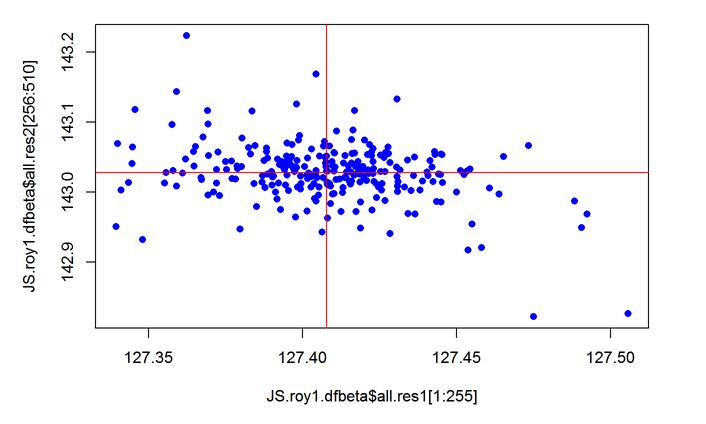
\includegraphics[width=0.7\linewidth]{images/dfbetas-JS-ROY}
	\caption{}
	\label{fig:dfbetas-JS-ROY}
\end{figure}







%---------------------------------------------------------------------------%
%---------------------------------------------------------------------------%


\section{Case Deletion Diagnostics} %1.6

\citet{CPJ} develops \index{case deletion diagnostics} case deletion diagnostics, in particular the equivalent of \index{Cook's distance} Cook's distance, for diagnosing influential observations when estimating the fixed effect parameters and variance components.

\section{Deletion Diagnostics}

Since the pioneering work of Cook in 1977, deletion measures have been applied to many statistical models for identifying influential observations.

Deletion diagnostics provide a means of assessing the influence of an observation (or groups of observations) on inference on the estimated parameters of LME models.

Data from single individuals, or a small group of subjects may influence non-linear mixed effects model selection. Diagnostics routinely applied in model building may identify such individuals, but these methods are not specifically designed for that purpose and are, therefore, not optimal. We describe two likelihood-based diagnostics for identifying individuals that can influence the choice between two competing models.

Case-deletion diagnostics provide a useful tool for identifying influential observations and outliers.

The computation of case deletion diagnostics in the classical model is made simple by the fact that estimates of $\beta$ and $\sigma^2$, which exclude the ith observation, can be computed without re-fitting the model. Such update formulas are available in the mixed model only if you assume that the covariance parameters are not affected by the removal of the observation in question. This is rarely a reasonable assumption.

\subsection*{3. Case Deletion Diagnostics for LME Data: Cooks Distance, DFBetas}
In this section we introduce influence analysis and case deletion diagnosics. A full overview of the topic will be provided although there are specific tools that are particularly useful in the case of MCS problems: specifically the Cook's Distance and the DFBeta.

A discussion of how leave-k-out diagnostics would work in the context of MCS problems is required. There are several scenaros. Suppose we have two methods of measurement X and Y, each with three measurements for a specific case: $(x_1,x_2,x_3,y_1,y_2,y_3)$

\begin{itemize}
	\item Leave One Out - one observation is omitted (e.g. $x_1$)
	\item Leave Pair Out - one pair of observation  is omitted (e.g. $x_1$ and $y_1$)
	\item Leave Case (or Subject) Out - All observations associated with a particular case or subject are omitted. (e.g. $\{x_1,x_2,x_3,y_1,y_2,y_3\}$)
\end{itemize}
Other metrics, such as the likelihood distance, will also be introduced, and revisited in a later section.
%========================================================= %
%- D
\newpage
\subsection*{4. Using DFBETAs to Assess Agreement}
Suppose an LME model was formulated to model agreement for various (i.e. 2 or more) methods of measurement, with replicate measurements. If the methods are to be agreement, the DFBetas for each case would be the same for both methods.\textbf{As such, agreement between any two methods can be determined by a simple scatterplot of the DFBetas. If the points align along the line of equality, then both methods can be said to be in agreement.}

%Cook's Distance can be used to identify and rank cases, in terms of influence.
For the model fitted to the blood data with the lme4 R package, the results tabulated below can be produced. All 85 subjects are ranked by Cook's Distance (with only the top 6 being presented here). The remaining columns are the DFBeta for each of the fixed effects, for each of the 85 subject.
\begin{center}
	\begin{tabular}{|c|c|c|c|c|} \hline
		Subject &    Cook's D  &    methodJ  &   methodR  & methodS \\ \hline \hline
		78 & 0.61557407 & -0.02934556 & -0.03387780 & 0.2954937  \\ \hline
		80 & 0.41590973 & -0.06305026 & -0.06515241 & 0.2123881  \\ \hline
		68 & 0.22536651 & -0.05334867 & -0.05062375 & 0.1555187  \\ \hline
		72 & 0.09348500  & 0.02388626  & 0.02419887 & 0.1617474  \\ \hline
		48 & 0.08706988  & 0.02147541  & 0.03145273 & 0.1581591  \\ \hline
		30 & 0.07118415  & 0.26925807  & 0.26215970 & 0.1581569  \\ \hline
	\end{tabular} 
\end{center}
\newpage
\begin{figure}[h!]
	\centering
	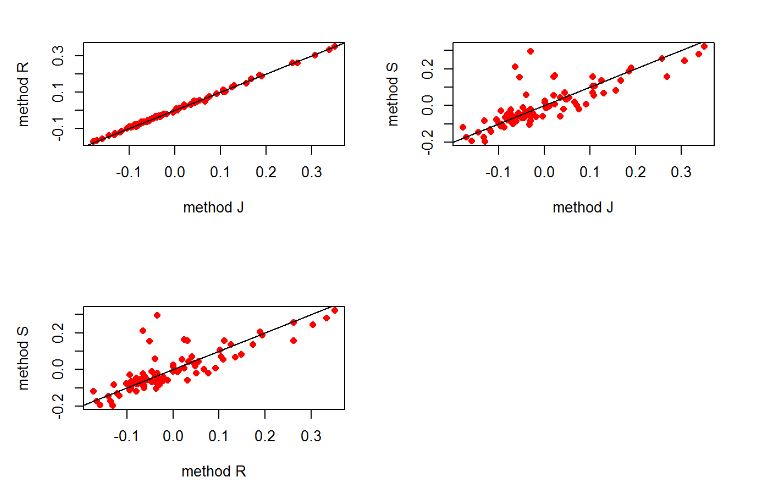
\includegraphics[width=0.9\linewidth]{images/04-DFbetaplots}
	% \caption{}
	% \label{fig:04-DFbetaplots}
\end{figure}

In the first of the three plots (\textit{Top Right}), strong agreement between method J and method R is indicated. The other plots indicate lack of agreement of methods J and R with method S.



If lack of agreement is indicated, a subsequent analysis using a technique proposed by Roy(2009) can be used to identify the specific cause for this lack of agreement (see next section).
\newpage

The Pearson Correlation coefficient of the DFBetas can be used in conjection with this analysis. A high correlation confirms good agreement. No threshold value for agreement is suggested, and analysts are advised to perform model diagnostics regardless of the correlation coeffient. 


The Bonferroni Outlier Test and Cook's Distance values can be used to identify unusual cases, when the relationship between sets of dfbeta is modelled as a (classical) linear model. In this model, the covariates should be homoskedastic. A test for non-constant variance may be used to verify this. These diagnostic procedures are implementable using the \textbf{\textit{car}} R package.

Deming Regression can be used to verify the line of equality. Significance test for Deming regression estimates are not available, but 95\% bootstrap confidence intervals for the slope estimate and intercept estimates can be computed. 


Additionally a mean difference plot can be used to identify outliers. This mean-difference plot differs from the Bland-Altman plot in that the plot is denominated in terms of dfbeta values, and not in measurement units.

If lack of agreement is indicated between methods of measurement, use of Roy's Testing is advised (This is the subject of the next section).
\begin{figure}[h1]
	\centering
	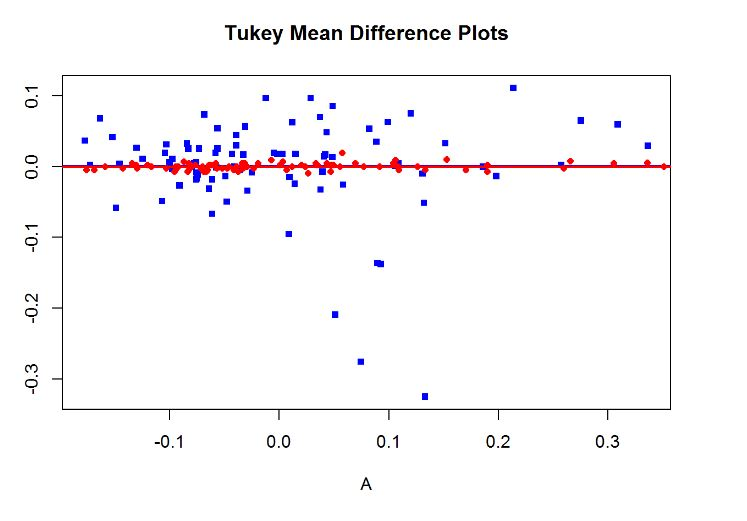
\includegraphics[width=0.7\linewidth]{images/04-TMDplot}
	\caption{}
	\label{fig:04-TMDplot}
\end{figure}
\newpage
%========================================================= %
%% - Part E
\subsection*{5. Using Roy's Test to Identify cause of Lack of agreement}

Barnhart specifies three conditions for method of measurement that are required for two methods of measurement to be considered in agreement.

\begin{itemize}
	\item[(i)] No Significant Inter-method bias
	\item[(ii)] No significant Difference in Within-Subject Variance
	\item[(iii)] No significant Difference in Within-Subject Variance 
\end{itemize}


Roy(2009) demonstrates a LME model specification, and a series of tests that look at each of these agreement criteria individually. If two methods of measuement lack agreement, the specific reason or reasons for this lack of agreement can be identified.


Roy proposes an LME model with Kronecker product covariance structure in a doubly multivariate setup. Response for $i$th subject can be written as
\[ y_i = \beta_0 + \beta_1x_{i1} + \beta_2x_{i2} + b_{1i}z_{i1}  + b_{2i}z_{i2} + \epsilon_i \]
\begin{itemize}
	\item $\beta_1$ and $\beta_2$ are fixed effects corresponding to both methods. ($\beta_0$ is the intercept.)
	\item $b_{1i}$ and $b_{2i}$ are random effects corresponding to both methods.
\end{itemize}

Overall variability between the two methods ($\Omega$) is sum of between-subject ($D$) and within-subject variability ($\Sigma$),
\[
\mbox{Block } \boldsymbol{\Omega}_i = \left[ \begin{array}{cc} d^2_1 & d_{12}\\ d_{12} & d^2_2\\ \end{array} \right]
+ \left[\begin{array}{cc} \sigma^2_1 & \sigma_{12}\\ \sigma_{12} & \sigma^2_2\\ \end{array}\right].
\]
%============================================== %
%- F:
\subsection*{6. Using Roy's Model to Compute LoAs and CR }

In this short section, a demonstration of how Roy's technique can be used to compute two common MCS metrics: Limits of Agreement and the Coefficient of Repeatabilty. While Limits of Agreement are not used in the analysis proposed here, they are ubiquituous in literature, and a demonstration on how to compute them with the Roy Model would assist the adoption of this proposed method.

The coefficient of repeatability is encountered in Gage R \& R analysis. \textit{(A future exploration of how LME models can be used in that field would be of interest. This is something to include in the Conclusions Section).}
%============================================== %
%- G:
\subsection*{7. Model Diagnostics for Roy's Models}

Further to previous work, this section revisits case-deletion and residual diagnostics, and explores how approaches devised by  Galecki \& Burzykowski (2013) can be used to appraise Roy's model. These authors specifically look at Cook's Distances and Likelihood Distances.
For the Roy Model, Cook's Distances may also be generated using the \textbf{\textit{predictmeans}}



\begin{figure}[h!]
	\centering
	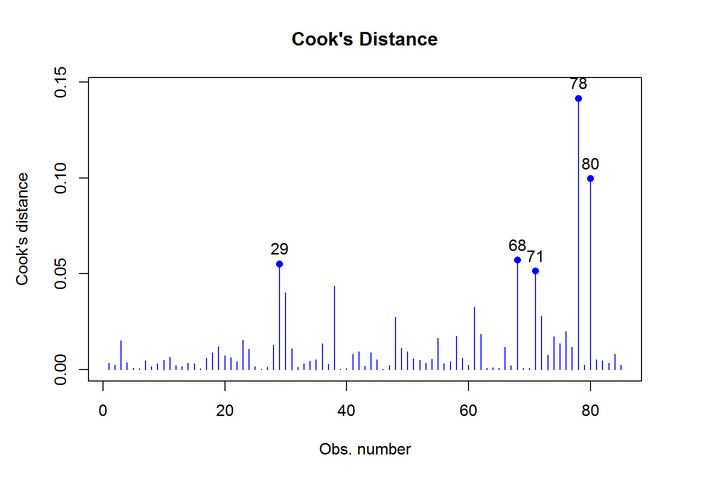
\includegraphics[width=0.7\linewidth]{images/CooksDistancePlot-JS-Roy}
	\caption{}
	\label{fig:CooksDistancePlot-JS-Roy}
\end{figure}

\begin{figure}[h!]
	\centering
	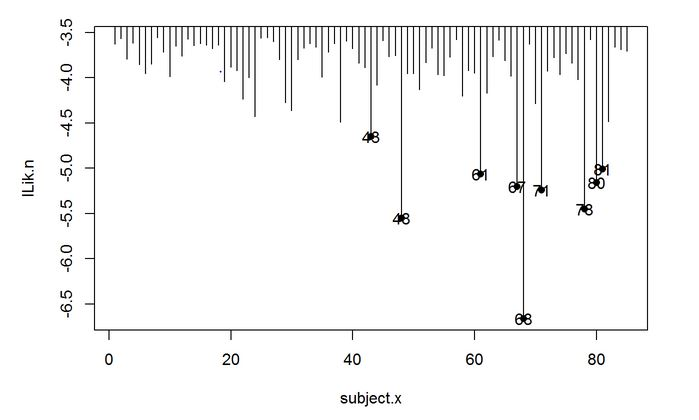
\includegraphics[width=0.7\linewidth]{images/LogLik-JS-Roy}
	\caption{}
	\label{fig:LogLik-JS-Roy}
\end{figure}

As the model is structurally different from the models discussed in the earlier sections, Residual analysis will be briefly revisited.
\begin{figure}[h!]
	\centering
	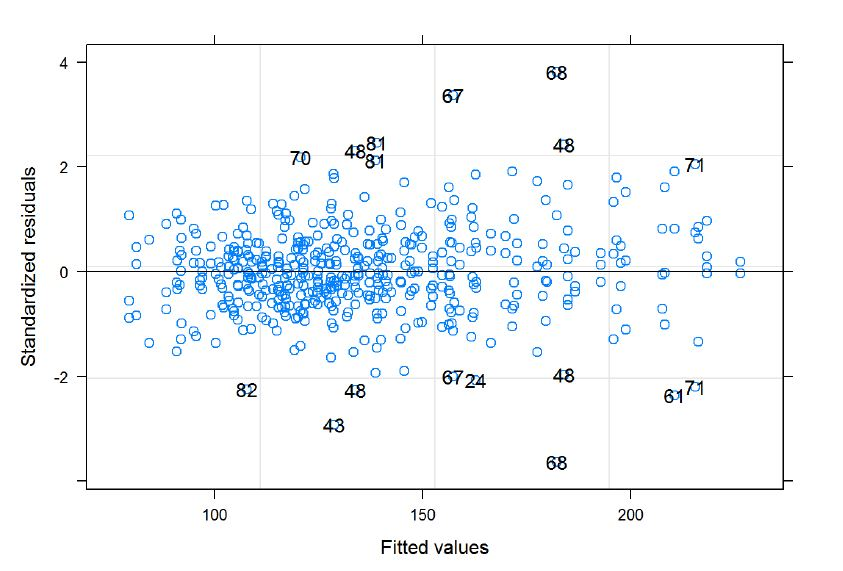
\includegraphics[width=0.7\linewidth]{images/Residuals-JS-Roy}
	\caption{}
	\label{fig:Residuals-JS-Roy}
\end{figure}

\newpage
\subsection*{8. Case Deletion Diagnostics for the Variance Ratios}
%- H Case Deletion Diagnostics 

Schabenberger advises on the use of deletion diagnostics for variance components of an LME model.
Taking the core principals of his methods, and applying them to the Method Comparison problem, case deletion diagnostics are used on the variance components of the Roy model., specifically the ratio of between subject variances and the within subject covariances respecitvely.


\[ \mbox{BSVR} = \frac{\sigma^2_2}{\sigma^2_2} \phantom{makespace}  \mbox{WSVR} = \frac{d^2_2}{d^2_2} \]

These variance ratios are re-computed for each case removed, and may be analysed seperately or jointly for outliers. 

The Grubbs' Test for Outliers is a commonly used technique for assessing outlier in a univariate data set. As there may be several outliers (i.e. influential cases) present, the Grubbs test is not practical. However outlier detection using to Tukey's 
specification for boxplots (i.e. greater than $Q_3 +1.5 IQR$ or less than $Q_1 - 1.5 IQR$), will suffice. Ranking the asbolute values of the standardizaed scores can also can be used to identify influential cases, even if the data is not normally distributed.

Bivariate Analyses may be applied jointly to the both sets of data sets, e.g Mahalanobis distances. The Mahalanobis distance, while not an intuitive measure in the context of the data, can be used to rank highly influential cases. 

%============================================== %
% - I: 
\subsection*{9. Permutation Test, Power Tests and Missing Data }

This section explores topics such as dependent variable simulation and power analysis, introduced by Galecki \& Burzykowski (2013), and implementable with their \textbf{\textit{nlmeU}} \texttt{R} package.
Using the \textbf{\textit{predictmeans}} \texttt{R} package, it is possible to perform permutation t-tests for coefficients of (fixed) effects and permutation F-tests.

The matter of missing data has not been commonly encountered in either Method Comparison Studies or Linear Mixed Effects Modelling. However Roy (2009) deals with the relevant assumptions regrading missing data. Galecki \& Burzykowski (2013) approaches the subject of missing data in LME Modelling. The \textbf{\textit{nlmeU}} package includes the \texttt{patMiss} function, which ``\textit{allows to compactly present pattern of missing data in a given vector/matrix/data
	frame or combination of thereof}".


%================================================%

%-------------------------------------------------------------------------------------------------------------------------------------%
\subsection{Influential Observations : DFBeta and DFBetas}
\section{Measures of Influence} %1.16

The impact of an observation, or a case with multiple obverations, on a regression fitting can be determined by the difference between the estimated regression coefficient of a model with all observations and the estimated coefficient when the particular observation is deleted. The measure DFBETA is the studentized value of this difference.


\section{Overall Influence}
An overall influence statistic measures the change in the objective function being minimized. For example, in
OLS regression, the residual sums of squares serves that purpose. In linear mixed models fit by
\index{maximum likelihood} maximum likelihood (ML) or \index{restricted maximum likelihood} restricted maximum likelihood (REML), an overall influence measure is the \index{likelihood distance} likelihood distance [Cook and Weisberg ].
%============================================================================= %

\section{Effects on fitted and predicted values}
\begin{equation}
	\hat{e_{i}}_{(U)} = y_{i} - x\hat{\beta}_{(U)}
\end{equation}

\section{Case Deletion Diagnostics for Mixed Models}

\citet{Christiansen} notes the case deletion diagnostics techniques have not been applied to linear mixed effects models and seeks to develop methodologies in that respect.

\citet{Christiansen} develops these techniques in the context of REML


\section{Terminology for Case Deletion diagnostics} %1.8

\citet{preisser} describes two type of diagnostics. When the set consists of only one observation, the type is called
'observation-diagnostics'. For multiple observations, Preisser describes the diagnostics as 'cluster-deletion' diagnostics.	\section{Case Deletion Diagnostics}
Case-deletion diagnostics provide a useful tool for identifying influential observations and outliers.

The computation of case deletion diagnostics in the classical model is made simple by the fact that estimates of $\beta$ and $\sigma^2$, which exclude the ith observation, can be computed without re-fitting the model. Such update formulas are available in the mixed model only if you assume that the covariance parameters are not affected by the removal of the observation in question. This is rarely a reasonable assumption.

Linear models for uncorrelated data have well established measures to gauge the influence of one or more
observations on the analysis. For such models, closed-form update expressions allow efficient computations
without refitting the model. 


Since the pioneering work of Cook in 1977, deletion measures have been applied to many statistical models for identifying influential observations. Case-deletion diagnostics provide a useful tool for identifying influential observations and outliers.

The key to making deletion diagnostics useable is the development of efficient computational formulas, allowing one to obtain the \index{case deletion diagnostics} case deletion diagnostics by making use of basic building blocks, computed only once for the full model.

The computation of case deletion diagnostics in the classical model is made simple by the fact that estimates of $\beta$ and $\sigma^2$, which exclude the $i-$th observation, can be computed without re-fitting the model. %\subsection{Terminology for Case Deletion diagnostics} %1.8

\citet{preisser} describes two type of diagnostics. When the set consists of only one observation, the type is called
`\textit{observation-diagnostics}'. For multiple observations, Preisser describes the diagnostics as `\textit{cluster-deletion}' diagnostics. When applied to LME models, such update formulas are available only if one assumes that the covariance parameters are not affected by the removal of the observation in question. However, this is rarely a reasonable assumption.
%--------------------------------------------------------------------------%
\newpage
\section{Case Deletion Diagnostics}

Since the pioneering work of Cook in 1977, deletion measures have been applied to many statistical models for identifying influential observations.

Deletion diagnostics provide a means of assessing the influence of an observation (or groups of observations) on inference on the estimated parameters of LME models.

Data from single individuals, or a small group of subjects may influence non-linear mixed effects model selection. Diagnostics routinely applied in model building may identify such individuals, but these methods are not specifically designed for that purpose and are, therefore, not optimal. We describe two likelihood-based diagnostics for identifying individuals that can influence the choice between two competing models.
Case-deletion diagnostics provide a useful tool for identifying influential observations and outliers.

The computation of case deletion diagnostics in the classical model is made simple by the fact that estimates of $\beta$ and $\sigma^2$, which exclude the ith observation, can be computed without re-fitting the model. Such update formulas are available in the mixed model only if you assume that the covariance parameters are not affected by the removal of the observation in question. This is rarely a reasonable assumption.

\section{Terminology for Case Deletion diagnostics} %1.8

\citet{preisser} describes two type of diagnostics. When the set consists of only one observation, the type is called
'observation-diagnostics'. For multiple observations, Preisser describes the diagnostics as 'cluster-deletion' diagnostics.
\section{influence.ME}

\textit{influence.ME} allows you to compute measures of influential data for mixed effects models generated by lme4.

\textit{influence.ME} provides a collection of tools for detecting influential cases in generalized mixed effects models. It analyses models that were estimated using lme4. The basic rationale behind identifying influential data is that when iteratively single units are omitted from the data, models based on these data should not produce substantially different estimates. 

To standardize the assessment of how influential a (single group of) observation(s) is, several measures of influence are common practice, such as DFBETAS and Cook's Distance. In addition, we provide a measure of percentage change of the fixed point estimates and a simple procedure to detect changing levels of significance.
\newpage

\section{Influence() command}
\texttt{influence()} is the workhorse function of the influence.ME package. Based on a priorly estimated mixed effects regression model (estimated using lme4), the \texttt{influence()} function iteratively modifies the mixed effects model to neutralize the effect a grouped set of data has on the parameters, and which returns returns the fixed parameters of these iteratively modified models. These are used to compute measures of influential data.
%============================================================================= %
\section{Cooks's Distance}
Cook's Distance is a measure indicating to what extent model parameters are influenced by (a set of) influential data on which the model is based. This function computes the Cook's distance based on the information returned by the estex() function.
%============================================================================= %
\chapter{Appendices 1}


\section{LME - Pankaj Choudhury}
Consistent with the conventions of mixed models, \citep{pkc}
formulates the measurement $y_{ij} $from method $i$ on individual
$j$ as follows;
\begin{equation}
	y_{ij} =P_{ij}\theta + W_{ij}v_{i} + X_{ij}b_{j} + Z_{ij}u_{j} +
	\epsilon_{ij},     (j=1,2, i=1,2....n)
\end{equation}
The design matrix $P_{ij}$ , with its associated column vector
$\theta$, specifies the fixed effects common to both methods. The
fixed effect specific to the $j$th method is articulated by the
design matrix $W_{ij}$ and its column vector $v_{i}$. The random
effects common to both methods is specified in the design matrix
$X_{ij}$, with vector $b_{j}$ whereas the random effects specific
to the $i$th subject by the $j$th method is expressed by $Z_{ij}$,
and vector $u_{j}$. Noticeably this notation is not consistent
with that described previously.  The design matrices are specified
so as to includes a fixed intercept for each method, and a random
intercept for each individual. Additional assumptions must also be
specified;
\begin{equation}
	v_{ij} \sim N(0,\Sigma),
\end{equation}
These vectors are assumed to be independent for different $i$s,
and are also mutually independent. All Covariance matrices are
positive definite.  In the above model effects can be classed as
those common to both methods, and those that vary with method.
When considering differences, the effects common to both
effectively cancel each other out. The differences of each pair of
measurements can be specified as following;
\begin{equation}
	d_{ij} = X_{ij}b_{j} + Z_{ij}u_{j} + \epsilon_{ij},     (j=1,2,
	i=1,2....n)
\end{equation}
This formulation has seperate distributional assumption from the
model stated previously.

This agreement covariate $x$ is the key step in how this
methodology assesses agreement.
%%%%%%%%%%%%%%%%%%%%%%%%%%%%%%%%%%%%%%%%%%%%%%%%%%%%%%%%%%%%%%%%%%%%%%%%%%%%%%%%%%%%%%%%%%%%%%%%%%%%%%%5
%----------------------------------------------------------------------------%
\newpage


\section{Model Terms (Roy 2009)}
\begin{itemize}
	\item Let $y_{mir}$ be the response of method $m$ on the $i$th subject
	at the $r-$th replicate.
	\item Let $\boldsymbol{y}_{ir}$ be the $2 \times 1$ vector of measurements
	corresponding to the $i-$th subject at the $r-$th replicate.
	\item Let $\boldsymbol{y}_{i}$ be the $R_i \times 1$ vector of
	measurements corresponding to the $i-$th subject, where $R_i$ is number of replicate measurements taken on item $i$.
	\item Let $\alpha_mi$ be the fixed effect parameter for method for subject $i$.
	\item Formally Roy uses a separate fixed effect parameter to describe the true value $\mu_i$, but later combines it with the other fixed effects when implementing the model.
	\item Let $u_{1i}$ and $u_{2i}$ be the random effects corresponding to methods for item $i$.
	
	\item $\boldsymbol{\epsilon}_{i}$ is a $n_{i}$-dimensional vector
	comprised of residual components. For the blood pressure data $n_{i} = 85$.
	
	\item $\boldsymbol{\beta}$ is the solutions of the means of the two methods. In the LME output, the bias ad corresponding
	t-value and p-values are presented. This is relevant to Roy's first test.\end{itemize}





%------------------------------------------------%
\newpage

\section{Algorithms}
Maximum likelihood estimation is a method of obtaining estimates
of unknown parameters by optimizing a likelihood function. The ML
parameter estimates are the values of the argument that maximise
the likelihood function, i.e. the estimates that make the observed
values of the dependent variable most likely, given the
distributional assumptions

The most common iterative algorithms used for the optimization
problem in the context of LMEs are the EM algoritm, fisher scoring
algorithm and NR algorithm, which [cite:West] commends as the
preferred method.

A mixed model is an extension of the general linear models that
can specify additional random effects terms.

Parameter of the mixed model can be estimated using either ML or
REML, while the AIC and the BIC can be used as measures of
"goodness of fit" for particular models, where smaller values are
considered preferable.

%--------------------------------------------------------------------%


\section{ML v REML}
(\textbf{\emph{Wikipedia}})The restricted (or residual, or reduced) maximum likelihood (REML) approach is a particular form of maximum likelihood estimation which does not base estimates on a maximum likelihood fit of all the information, but instead uses a likelihood function calculated from a transformed set of data, so that nuisance parameters have no effect.

In contrast to the earlier maximum likelihood estimation, REML can produce unbiased estimates of variance and covariance parameters.

%-----------------------------------------------------------------------------------------%
\newpage
\section{ML procedures for LME}

The maximum likelihood procedure of Hartley and Rao yields
simultaneous estimates for both the fixed effects and the random
effect, by maximising the likelihood of $\boldsymbol{y}$ with
respect to each element of $\boldsymbol{\beta}$ and
$\boldsymbol{b}$.

%-----------------------------------------------------------------------------------------%
\newpage
\section{Estimation of random effects}

Estimation of random effects for LME models in the NLME package is accomplished through use
of both EM (Expectation-Maximization) algorithms and Newton-Raphson algorithms.
\begin{itemize}
	\item EM iterations bring estimates of the parameters into the region of the optimum very quickly, but
	convergence to the optimum is slow when near the optimum.
	\item Newton-Raphson iterations are computationally intensive and can be unstable when far from the
	optimum. However, close to the optimum they converge quickly.
	\item The LME function implements a hybrid approach, using 25 EM iterations to quickly get near the
	optimum, then switching to Newton-Raphson iterations to quickly converge to the optimum. \item If
	convergence problems occur, the ``control� argument in LME can be used to change the way the
	model arrives at the optimum.
\end{itemize}







%------------------------------------------------%
\newpage

%===================================================================================== %
\newpage
\bibliography{DB-txfrbib}
\end{document}
%---------------------------------------------------------------------------------------------------%


